\documentclass[twoside]{book}
\setcounter{tocdepth}{1}
\usepackage[a4paper,
    inner=4cm,  % Inner margin (binding side)
    outer=3.5cm,  % Outer margin
    top=3cm,
    bottom=3cm
]{geometry}
\usepackage[hidelinks]{hyperref}
%\usepackage{mathpazo}
%\usepackage{newtxtext,newtxmath}
\usepackage{amsmath}
\usepackage{amssymb}
\allowdisplaybreaks[1]
\usepackage{multirow}
\usepackage{rotating}
\usepackage{booktabs}
\usepackage{rotating}
\usepackage{tikz}
\usepackage{fancyhdr}
\usepackage{enumitem}
\usepackage{tabularx}
\usepackage{booktabs}
\usepackage[utf8]{inputenc}
\usepackage{tcolorbox}
\setlength{\parindent}{0pt}
\setlength{\parskip}{6pt}
\usepackage{tikz}
\usetikzlibrary{shapes.geometric, arrows.meta, positioning}
\usepackage{pgfplots}
\usepackage{pgf-pie}
\pgfplotsset{compat=1.18}
\usepgfplotslibrary{groupplots}
\usetikzlibrary{fillbetween,patterns,shapes,arrows.meta}
\usetikzlibrary{calc}
\usetikzlibrary{arrows.meta}
\tikzstyle{startstop} = [rectangle, rounded corners, minimum width=3cm, minimum height=1cm,text centered, draw=black, fill=gray!10]
\tikzstyle{arrow} = [thick,->,>=stealth]
\usepackage{subcaption}
\pgfplotsset{compat=1.17}
\usepackage{caption}
\usepackage{booktabs}
\usepackage{array}
\usepackage{float}
\pagestyle{fancy}
\fancyhf{}
\fancyfoot[C]{\thepage}
\renewcommand{\headrulewidth}{0pt}
\tcbset{
  heading/.style={
    colback=white,
    colframe=gray!95!white,
    fonttitle=\bfseries,
    title=#1
  }
}
\newtcolorbox{textbox}[1][]{%
  colback=white,
  colframe=gray!95!white,
  #1
}
\usepackage{listings}
\usepackage{xcolor}
\definecolor{dkgreen}{rgb}{0,0.6,0}
\definecolor{gray}{rgb}{0.5,0.5,0.5}
\definecolor{mauve}{rgb}{0.58,0,0.82}
\lstset{frame=tb,
	language=Python,
	aboveskip=3mm,
	belowskip=3mm,
	showstringspaces=false,
	columns=flexible,
	basicstyle={\small\ttfamily\bfseries},
	numbers=none,
	numberstyle=\tiny\color{gray},
	keywordstyle=\color{blue},
	commentstyle=\color{dkgreen},
	stringstyle=\color{mauve},
	breaklines=true,
	breakatwhitespace=true,
	tabsize=3,
	upquote=true,
	numbers=left,
	firstnumber=1,
	numberfirstline=true
}
\newcommand{\largedot}{\raisebox{0.1pt}{\scalebox{1.5}{$\cdot$}}}
\newcommand{\tallymark}[1]{%
  \begin{tikzpicture}[scale=0.2,baseline]
    \pgfmathtruncatemacro{\n}{#1}
    \foreach \i in {1,...,\n} {
      \pgfmathtruncatemacro{\group}{int((\i-1)/5)} % group number: 0 for 1–5, 1 for 6–10, etc.
      \pgfmathtruncatemacro{\posingroup}{mod(\i-1,5) + 1} % position in group: 1 to 5

      \pgfmathsetmacro{\xshift}{\group * 6} % 6 units between groups

      \ifnum\posingroup=5
        \draw[thick] (\xshift+0.8,0) -- (\xshift+4.2,4); % cross-line
      \else
        \pgfmathsetmacro{\x}{\xshift + \posingroup}
        \draw[thick] (\x,0) -- (\x,4); % vertical lines
      \fi
    }
  \end{tikzpicture}
}

\usepackage{tocloft}

\usepackage{titlesec}
\usepackage{etoolbox}

\definecolor{myblue}{RGB}{0, 102, 204}

% CHAPTER, SECTION, SUBSECTION TITLES IN BLUE
\titleformat{\chapter}[display]
  {\normalfont\Huge\bfseries\color{myblue}}{\chaptername\ \thechapter}{20pt}{\Huge}
\titleformat{\section}
  {\normalfont\Large\bfseries\color{myblue}}{\thesection}{1em}{}
\titleformat{\subsection}
  {\normalfont\large\bfseries\color{myblue}}{\thesubsection}{1em}{}

% adjust the width reserved for the sec‐number, if you need more room:
\setlength{\cftsecnumwidth}{3em}

% insert a quad (≈1 em) after the number and before the title
\renewcommand{\cftsecaftersnum}{\quad}

% vertical gap *before* each section entry (here: half a line)
\setlength{\cftbeforesecskip}{0.5\baselineskip}

\title{Fundamentals of Probability and Statistics}
\author{Sandip Karar}
\date{\today}


\begin{document}

\begin{titlepage}
    \centering
    \vspace*{3cm}

    \begin{tikzpicture}[remember picture,overlay]
        % Draw a thin decorative frame around the page content area
        \draw[line width=1.5pt]
            ($(current page.north west)+(3cm,-2.5cm)$) rectangle ($(current page.south east)+(-2.5cm,2.5cm)$);
        \draw[line width=1.5pt]
            ($(current page.north west)+(2.7cm,-2.2cm)$) rectangle ($(current page.south east)+(-2.2cm,2.2cm)$);

    \end{tikzpicture}

    {\fontsize{24pt}{28pt}\bfseries\scshape Basics of Probability and Statistics\par}
    \vspace{1.2cm}


    {\Large\itshape An In-Depth Exploration of Core Concepts and Methods\par}

    \vspace{2cm}

    {\large\bfseries Sandip Karar\par}
    \vspace{0.5cm}

    {\normalsize\today\par}
    \vspace{2cm}

      \begin{center}
        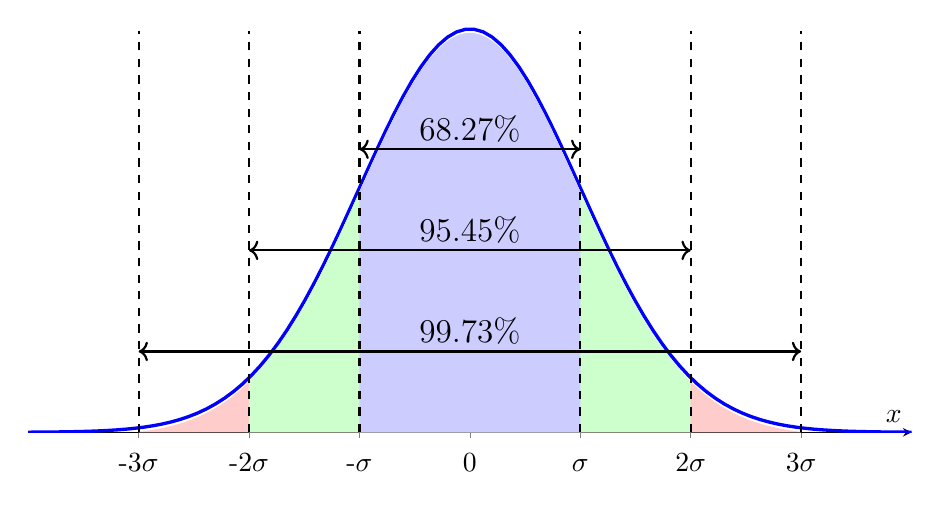
\begin{tikzpicture}
            \begin{axis}[
                no markers, domain=-4:4, samples=100,
                axis lines=center,
                xlabel={$x$},
                axis y line=none,
                ymin=0, ymax=0.5,
                xmin=-4, xmax=4,
                height=8cm, width=12.8cm,
                ytick=\empty,
                xtick={-3,-2,-1,0,1,2,3},
                xticklabels={-3$\sigma$,-2$\sigma$,-$\sigma$,0,$\sigma$,2$\sigma$,3$\sigma$},
                xticklabel style={
                	text height=2ex,
                	text depth=0.25ex
                },
              ]
              % PDF curve
              \addplot [very thick, blue] {1/sqrt(2*pi)*exp(-x^2/2)};
              % Shaded right-tail for z>1.5


              \addplot [draw=none, fill=red!20, domain=-3:3] {1/sqrt(2*pi)*exp(-x^2/2)-0.004} \closedcycle;
              % Vertical guide line
              \draw[thick, dashed] (axis cs:-3,0) -- (axis cs:-3,{1/sqrt(2*pi)*exp(-0.1^2/2)});
              \draw[thick, dashed] (axis cs:3,0) -- (axis cs:3,{1/sqrt(2*pi)*exp(-0.1^2/2)});


              \addplot [draw=none, fill=green!20, domain=-2:2] {1/sqrt(2*pi)*exp(-x^2/2)-0.004} \closedcycle;
              % Vertical guide line
              \draw[thick, dashed] (axis cs:-2,0) -- (axis cs:-2,{1/sqrt(2*pi)*exp(-0.1^2/2)});
              \draw[thick, dashed] (axis cs:2,0) -- (axis cs:2,{1/sqrt(2*pi)*exp(-0.1^2/2)});

              \addplot [draw=none, fill=blue!20, domain=-1:1] {1/sqrt(2*pi)*exp(-x^2/2)-0.004} \closedcycle;
              % Vertical guide line
              \draw[thick, dashed] (axis cs:-1,0) -- (axis cs:-1,{1/sqrt(2*pi)*exp(-0.1^2/2)});
              \draw[thick, dashed] (axis cs:1,0) -- (axis cs:1,{1/sqrt(2*pi)*exp(-0.1^2/2)});

              \node at (axis cs:0,0.3) {\large $68.27\%$};
              \node at (axis cs:0,0.2) {\large $95.45\%$};
              \node at (axis cs:0,0.1) {\large $99.73\%$};

              \draw[<->, thick, black] (axis cs:-3,0.08) -- (axis cs:3,0.08);
              \draw[<->, thick, black] (axis cs:-2,0.18) -- (axis cs:2,0.18);
              \draw[<->, thick, black] (axis cs:-1,0.28) -- (axis cs:1,0.28);
            \end{axis}
          \end{tikzpicture}
      \end{center}

\end{titlepage}

%\maketitle

\tableofcontents

\chapter{Descriptive Statistics}

\section{Introduction}

\href{https://bookdown.org/egarpor/inference/estmeth-mm.html}{https://bookdown.org/egarpor/inference/estmeth-mm.html}

Statistics is a branch of mathematics that deals with the collection, organization, analysis, interpretation, and presentation of data. It provides tools for making informed decisions in the presence of uncertainty.

\subsection{Uses of Statistics}

Statistics is widely used in various fields such as:

\begin{itemize}
    \item \textbf{Education}: Analyzing student performance and improving teaching methods.
    \item \textbf{Business}: Making informed decisions based on market trends and consumer behavior.
    \item \textbf{Healthcare}: Understanding the effectiveness of treatments and tracking disease outbreaks.
    \item \textbf{Government}: Planning and policy-making based on population data.
\end{itemize}

\subsection{Types of Data}

Data can be categorized based on their nature and measurement levels.

\textbf{1. Qualitative (Categorical) Data}

These are non-numeric data that describe categories or groups.

\begin{itemize}
    \item \textbf{Nominal}: Categories without any inherent order (e.g., colors, gender).
    \item \textbf{Ordinal}: Categories with a meaningful order but no fixed interval between them (e.g., rankings).
\end{itemize}

\textbf{2. Quantitative (Numerical) Data}

These are numeric data representing counts or measurements.

\begin{itemize}
    \item \textbf{Discrete}: Countable values (e.g., number of students).
    \item \textbf{Continuous}: Measurable quantities that can take any value within a range (e.g., height, weight).
\end{itemize}

\subsection{Data Collection Methods}

Collecting accurate data is crucial for meaningful analysis. Common methods include:

\begin{itemize}
    \item \textbf{Surveys}: Gathering information through questionnaires.
    \item \textbf{Experiments}: Conducting controlled studies to observe outcomes.
    \item \textbf{Observations}: Recording data based on direct observation.
    \item \textbf{Existing Records}: Utilizing previously collected data.
\end{itemize}

Tally for 3: \tallymark{3} \\
Tally for 5: \tallymark{5} \\
Tally for 7: \tallymark{7}

\subsection{Organizing Data}

Once data is collected, organizing it helps in understanding patterns and trends.

\textbf{1. Frequency Distribution Table}

A frequency distribution table lists data values and their corresponding frequencies.

\begin{table}[h]
\centering
\begin{tabular}{c|c}
\hline
\textbf{Number of Books} & \textbf{Number of Students} \\
\hline
0--2 & 5 \\
3--5 & 12 \\
6--8 & 17 \\
9--11 & 8 \\
12--14 & 3 \\
\hline
\end{tabular}
\caption{Number of Books Read by Students}
\end{table}

\textbf{2. Relative Frequency}

Relative frequency represents the proportion of observations within each category.

\begin{table}[h]
\centering
\begin{tabular}{c|c}
\hline
\textbf{Number of Books} & \textbf{Relative Frequency} \\
\hline
0--2 & 0.10 \\
3--5 & 0.24 \\
6--8 & 0.34 \\
9--11 & 0.16 \\
12--14 & 0.06 \\
\hline
\end{tabular}
\caption{Relative Frequency of Books Read}
\end{table}

\subsection{Displaying Data}

Visual representations make it easier to comprehend data.

\textbf{1. Bar Graph}

Bar graphs are used for categorical data.

\begin{figure}[H]
\centering
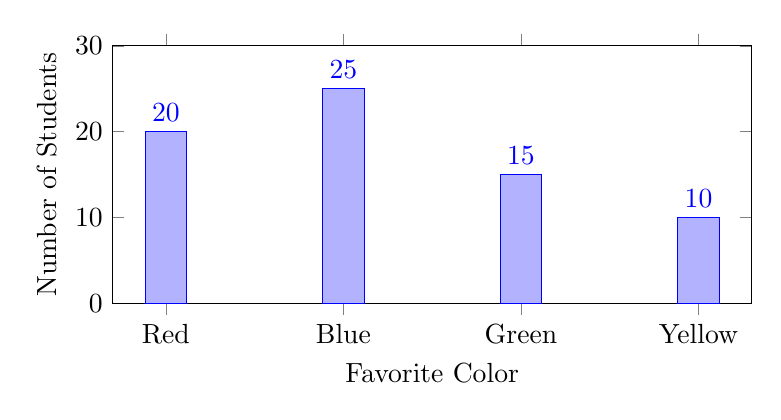
\begin{tikzpicture}
\begin{axis}[
    ybar,
    symbolic x coords={Red, Blue, Green, Yellow},
    xtick=data,
    ylabel={Number of Students},
    xlabel={Favorite Color},
    ymin=0,
    ymax=30,
    bar width=15pt,
    nodes near coords,
    width=0.8\textwidth,
    height=0.4\textwidth
]
\addplot coordinates {(Red,20) (Blue,25) (Green,15) (Yellow,10)};
\end{axis}
\end{tikzpicture}
\caption{Favorite Colors of Students}
\end{figure}

\textbf{2. Pie Chart}

Pie charts show the proportion of categories within a whole.

\begin{figure}[H]
\centering
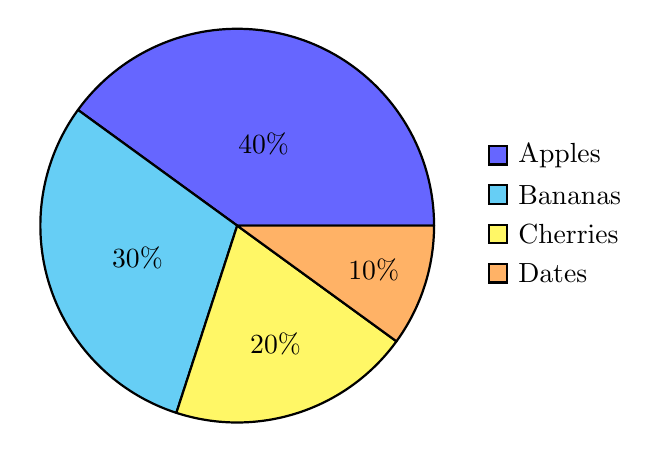
\begin{tikzpicture}
\pie[text=legend, radius=2.5]{40/Apples, 30/Bananas, 20/Cherries, 10/Dates}
\end{tikzpicture}
\caption{Fruit Preferences}
\end{figure}

\textbf{3. Histogram}

Histograms are used for continuous numerical data.

\begin{figure}[H]
\centering
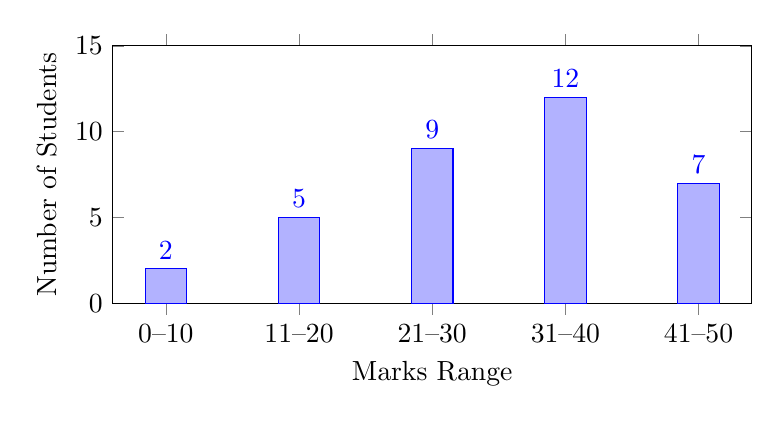
\begin{tikzpicture}
\begin{axis}[
    ybar,
    ymin=0,
    ymax=15,
    xlabel={Marks Range},
    ylabel={Number of Students},
    xtick=data,
    symbolic x coords={0--10,11--20,21--30,31--40,41--50},
    bar width=15pt,
    nodes near coords,
    width=0.8\textwidth,
    height=0.4\textwidth
]
\addplot coordinates {(0--10,2) (11--20,5) (21--30,9) (31--40,12) (41--50,7)};
\end{axis}
\end{tikzpicture}
\caption{Distribution of Marks}
\end{figure}

\textbf{4. Line Graph}

Line graphs depict data trends over time.

\begin{figure}[H]
\centering
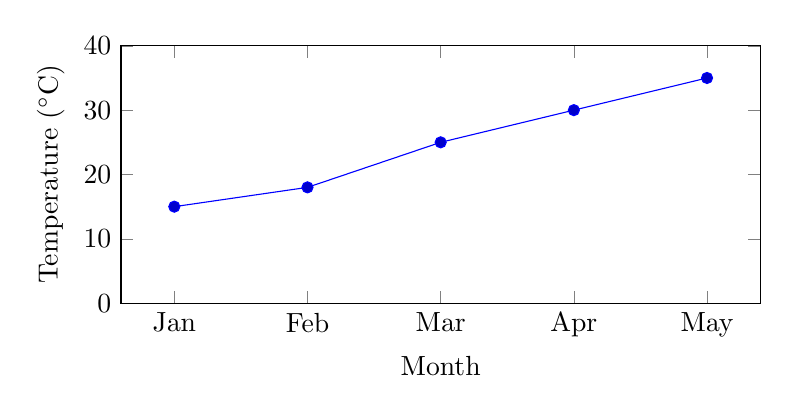
\begin{tikzpicture}
\begin{axis}[
    xlabel={Month},
    ylabel={Temperature ($^\circ$C)},
    xtick=data,
    symbolic x coords={Jan, Feb, Mar, Apr, May},
    ymin=0,
    ymax=40,
    width=0.8\textwidth,
    height=0.4\textwidth
]
\addplot coordinates {(Jan,15) (Feb,18) (Mar,25) (Apr,30) (May,35)};
\end{axis}
\end{tikzpicture}
\caption{Monthly Average Temperature}
\end{figure}

\section{Measures of Central Tendency}

Quite often, data exhibit a tendency to cluster around a central value. Measures of central tendency are numerical indicators that describe this central value of a data set. The most common measures include the mean, median, and mode. Each measure tells us something different about our data, and knowing when to use each one can really help us make sense of the numbers.

% \begin{center}
% \begin{tikzpicture}[
%   level 1/.style={sibling distance=30mm, level distance=20mm},
%   level 2/.style={sibling distance=45mm, level distance=20mm},
%   every node/.style={rectangle, draw=black, align=center, minimum width=2cm, minimum height=1cm}
%   ]

% \node {Measures of Central Tendency}
%   child {node {Mean}
%     child {node {Arithmetic Mean (AM)}}
%     child {node {Geometric Mean (GM)}}
%     child {node {Harmonic Mean (HM)}}
%   }
%   child {node {Median}}
%   child {node {Mode}};

% \end{tikzpicture}
% \end{center}

\begin{center}
    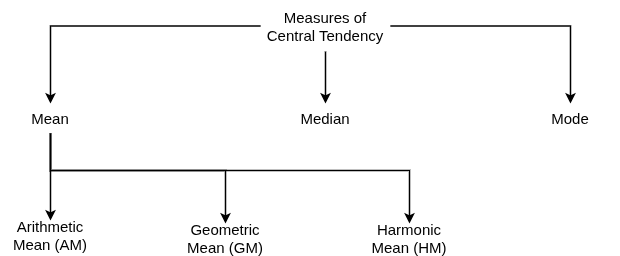
\includegraphics[scale=0.5]{pic/moct.drawio.png}
\end{center}

\subsection{Mean}

The mean (or average) is the most commonly used measure of central tendency and is defined in several forms:

\begin{itemize}
    \item \textbf{Arithmetic Mean (AM):}
    \begin{itemize}
        \item Simple AM: For a dataset \( x_1, x_2, \dots, x_n \), the arithmetic mean is given by:
    \begin{textbox}
    \[
    \overline{x} = \dfrac{1}{n} \sum_{i=1}^{n} x_i
    \]
    \end{textbox}
    \item Weighted AM: When each value \( x_i \) has an associated frequency \( f_i \), the weighted arithmetic mean is:
    \begin{textbox}
    \[
    \overline{x} = \dfrac{\sum_{i=1}^{n} f_i x_i}{\sum_{i=1}^{n} f_i}
    \]
    \end{textbox}
    \end{itemize}

\begin{textbox}
        \textbf{Theorem}: If \( x_i = a \) (constant) for all \( i \), then the arithmetic mean is also \( a \), that is,
\[
\overline{x} = a.
\]
\end{textbox}

\textbf{Proof:}
\begin{align*}
\overline{x} &= \frac{1}{n} \sum_{i=1}^n x_i
       = \frac{1}{n} \sum_{i=1}^n a = \frac{1}{n} \cdot n a = a
\end{align*}
\hfill $\blacksquare$

\begin{textbox}
\textbf{Theorem}: If \( y_i = a + x_i \), then the mean of \( y \) is given by:
\[
\overline{y} = a + \overline{x}.
\]
\end{textbox}

\textbf{Proof:}
\begin{align*}
\overline{y} &= \frac{1}{n} \sum_{i=1}^n y_i = \frac{1}{n} \sum_{i=1}^n (a + x_i) = \frac{1}{n} \left( \sum_{i=1}^n a + \sum_{i=1}^n x_i \right) \\
       &= \frac{1}{n} \left( n a + \sum_{i=1}^n x_i \right) = a + \overline{x}.
\end{align*}
\hfill $\blacksquare$

\begin{textbox}
\textbf{Theorem}: Let a dataset be composed of two distinct groups of observations:

\begin{itemize}
  \item Group 1 consists of \( n_1 \) observations with arithmetic mean \( \overline{x}_1 \),
  \item Group 2 consists of \( n_2 \) observations with arithmetic mean \( \overline{x}_2 \).
\end{itemize}

Then, the arithmetic mean \( \overline{x} \) of the combined dataset (of size \( n_1 + n_2 \)) is given by:
\[
\overline{x} = \dfrac{n_1 \overline{x}_1 + n_2 \overline{x}_2}{n_1 + n_2}.
\]
\end{textbox}

\textbf{Proof}: \text{Total sum of group 1} is $n_1 \overline{x}_1$ and \text{total sum of group 2} is $n_2 \overline{x}_2$.

Then total sum = $n_1 \overline{x}_1 + n_2 \overline{x}_2$

\text{Total number of observations} = $n_1 + n_2$

Therefore, combined AM = $\overline{x} = \dfrac{\text{Total sum}}{\text{Total number of observations}} \dfrac{n_1 \overline{x}_1 + n_2 \overline{x}_2}{n_1 + n_2}$

\hfill $\blacksquare$

    \item \textbf{Geometric Mean (GM):} Geometric mean of a set of $n$ observation is the $n$th root of their product. It is only defined for positive values.

    \begin{itemize}
        \item Simple GM:
        \begin{textbox}
    \[
    x_G = \left( \prod_{i=1}^{n} x_i \right)^{1/n} = \sqrt[n]{x_1 x_2 \dots x_n}
    \]
    \end{textbox}
    \item Weighted GM:
    \begin{textbox}
    \[
    x_G = \left( \prod_{i=1}^{n} x_i^{f_i} \right)^{1/N} = \sqrt[N]{x_1^{f_1} x_2^{f_2} \dots x_n^{f_n}}
    \]
    \end{textbox}
    \end{itemize}
    Where $$N = \sum_{i=1}^n f_i$$

        \begin{textbox}
        \textbf{Theorem}: The GM of a set of positive values \( x_1, x_2, \dots, x_n \) is equal to the antilogarithm (exponential) of the AM of their logarithms:
\[
\mathrm{GM} = \exp\left( \frac{1}{n} \sum_{i=1}^n \log x_i \right)
\]
    \end{textbox}

\textbf{Proof:}
\begin{align*}
\mathrm{GM} &= \left( \prod_{i=1}^n x_i \right)^{1/n} = \exp\left( \log \left( \prod_{i=1}^n x_i \right)^{1/n} \right) \\
            &= \exp\left( \frac{1}{n} \log \left( \prod_{i=1}^n x_i \right) \right) = \exp\left( \frac{1}{n} \sum_{i=1}^n \log x_i \right)
\end{align*}
\hfill $\blacksquare$

\begin{textbox}
\textbf{Theorem}: Suppose we have two groups:
\begin{itemize}
  \item Group 1 has \( N_1 \) positive values with geometric mean \( x_{G_1} \),
  \item Group 2 has \( N_2 \) positive values with geometric mean \( x_{G_2} \).
\end{itemize}
Then the combined geometric mean \( \mathrm{GM} \) of all \( N_1 + N_2 \) values is:
\[
\mathrm{GM} = \left( x_{G_1}^{N_1} \cdot x_{G_2}^{N_2} \right)^{1/(N_1 + N_2)}
\]
\end{textbox}

\textbf{Proof}: Let the product of values in group 1 be \( P_1 = \prod_{i=1}^{N_1} x_i \), so that:
\[
x_{G_1} = \left( P_1 \right)^{1/N_1} \Rightarrow P_1 = x_{G_1}^{N_1}
\]

Similarly, for group 2:
\[
P_2 = \prod_{j=1}^{N_2} y_j = x_{G_2}^{N_2}
\]

Then the overall product:
\[
P = P_1 \cdot P_2 = x_{G_1}^{N_1} \cdot x_{G_2}^{N_2}
\]

The combined GM is:
\begin{align*}
\mathrm{GM} &= \left( P \right)^{1/(N_1 + N_2)} = \left( x_{G_1}^{N_1} \cdot x_{G_2}^{N_2} \right)^{1/(N_1 + N_2)}
\end{align*}

\hfill $\blacksquare$

    \item \textbf{Harmonic Mean (HM):} Harmonic Mean of a set of observations is the reciprocal of the arithmetic mean of the reciprocals.
    \begin{itemize}
        \item Simple HM:
        \begin{textbox}
    \[
    x_H = \dfrac{1}{ \dfrac{1}{n}\displaystyle \sum_{i=1}^{n} \dfrac{1}{x_i}} = \dfrac{n}{\displaystyle \sum_{i=1}^{n} \dfrac{1}{x_i}}
    \]
    \end{textbox}
    \item Weighted HM:
    \begin{textbox}
    \[
    x_H = \dfrac{1}{ \dfrac{1}{N}\displaystyle \sum_{i=1}^{n} \dfrac{f_i}{x_i}} = \dfrac{N}{\displaystyle \sum_{i=1}^{n} \dfrac{f_i}{x_i}}
    \]
    \end{textbox}
    \end{itemize}

\end{itemize}

It is important to note where to use GM and where to use HM. GM is useful for averaging \textbf{ratios}, \textbf{rates} and \textbf{percentages}. As an illustration, we consider the following example.


\textbf{Example}: The ratio of the prices in 1994 and to those in 1982 for four commodities are $0.92, 1.25, 1.75$ and $0.85$. To get the average price ratio use geometric mean
\begin{align*}
    \log x_G &= \frac{1}{n}\left(\log 0.92+ \log 1.25+ \log 1.75 + \log 0.85\right)\\
    &= 0.5829 = \log 1.1436 \\
    \Rightarrow x_G &= 1.1436
\end{align*}


GM is also useful if one wants to determine the values of a variable at the midpoint of a time interval when the variable changes over time exponentially. Thus if the value at two points $0$ and $t$ be $a$ and $ar^t$, then its value at the midpoint $\frac{t}{2}$ is $(a \times ar^t)^{1/2} = ar^{t/2}$.

Now consider the following example:

\textbf{Example}: A person goes from $X$ to $Y$ on cycle at $20$ km/h and returns at $24$ km/h. What is the average speed for the entire trip?

If we use AM, then the average speed is
$$\frac{1}{2}(20+24) = 22 \text{ km/h}$$
But is this correct?

Consider the total distance between $X$ and $Y$ is $1$ km for the sake of simplicity. So the total distance covered = $2$ km. The time taken for the person to go from $X$ to $Y$ is $\frac{1}{20} = 0.05$ hr and the time taken to return is $\frac{1}{24} = 0.04166$ hr.

Therefore average speed = $\dfrac{\text{Total distance}}{\text{Total time}} = \dfrac{2}{0.05+0.04166} = 21.8$ km/h.

Clearly, the AM value of $22$ km/h overestimates the actual average speed. Now consider the harmonic mean (HM) of the two speeds: $$\dfrac{2}{\frac{1}{20}+\frac{1}{24}} = 21.8 \text{ km/h}$$

This matches the correct value.

Now where to use the HM? The harmonic mean is particularly useful when dealing with quantities expressed in the form ``$x$ per unit $y$'', such as ``km per hour'', ``rupees per kg'', and similar rates. Here $x$ and $y$ are unit of measures, not numeric variables.

\medskip

\begin{textbox}
\textbf{Rule of Thumb:}
\begin{itemize}
    \item Use the \textbf{harmonic mean (HM)} when equal quantities of $x$ are involved.
    \item Use the \textbf{arithmetic mean (AM)} when equal quantities of $y$ are involved.
\end{itemize}
\end{textbox}

\medskip

This principle can be illustrated with the following example.

\textbf{Example}: Suppose a train covers \textbf{\( n \) equal distances}, each of \( s \) kilometers, with speeds \( v_1, v_2, \dots, v_n \) km/h. The average speed is the total distance divided by the total time taken. Thus,

\[
\text{Average speed} = \dfrac{ns}{\dfrac{s}{v_1} + \dfrac{s}{v_2} + \dots + \dfrac{s}{v_n}}
= \frac{n}{\frac{1}{v_1} + \dfrac{1}{v_2} + \dots + \frac{1}{v_n}}
= \dfrac{n}{\displaystyle \sum_{i=1}^n \dfrac{1}{v_i}}
\]

This is the \textbf{harmonic mean (HM)} of the given speeds.

\medskip

On the other hand, if the train travels for \textbf{\( n \) equal time intervals}, each of duration \( t \) hours, at speeds \( v_1, v_2, \dots, v_n \) km/h, then the total distance covered is:

\[
\text{Total distance} = v_1t + v_2t + \dots + v_nt = t(v_1 + v_2 + \dots + v_n)
\]

and the total time is \( nt \). So, the average speed is:

\[
\text{Average speed} = \frac{t(v_1 + v_2 + \dots + v_n)}{nt} = \frac{v_1 + v_2 + \dots + v_n}{n}
= \frac{1}{n} \sum_{i=1}^n v_i
\]

which is the \textbf{arithmetic mean (AM)} of the given speeds.


\begin{textbox}
    \textbf{Theorem}: The sum of squared deviations from a constant \( A \) is minimized when \( A \) equals the arithmetic mean \( \overline{x} \), i.e.,

\[
\sum_{i=1}^n (x_i - A)^2 \text{ is minimized when } A = \overline{x}
\]
\end{textbox}

\textbf{Proof}: Let \( S(A) = \sum_{i=1}^n (x_i - A)^2 \). Expand this:

\[
S(A) = \sum_{i=1}^n (x_i^2 - 2Ax_i + A^2)
= \sum x_i^2 - 2A\sum x_i + nA^2
\]

To minimize \( S(A) \), take derivative with respect to \( A \) and set it to zero:

\[
\frac{dS}{dA} = -2\sum x_i + 2nA = 0 \quad \Rightarrow \quad A = \frac{1}{n} \sum x_i = \overline{x}
\]

Now, take the second derivative:

\[
\frac{d^2S}{dA^2} = 2n > 0
\]

Since the second derivative is positive, the function \( S(A) \) has a minimum at \( A = \overline{x} \).

\hfill $\blacksquare$

\begin{textbox}
\textbf{Theorem}: For two observations, \[ \text{GM}^2 = \text{AM} \times \text{HM} \]
\end{textbox}

\textbf{Proof}: Let \( a \) and \( b \) be two observations (positive numbers).

Compute left-hand side:

\[
\text{GM}^2 = (\sqrt{ab})^2 = ab
\]

Compute right-hand side:

\[
\text{AM} \times \text{HM} = \left( \frac{a + b}{2} \right) \left( \frac{2ab}{a + b} \right) = ab
\]

Hence, \[ \text{GM}^2 = \text{AM} \times \text{HM} \]
\hfill $\blacksquare$

\begin{textbox}
\textbf{Theorem}: For any set of \( n \) positive real numbers \( x_1, x_2, \dots, x_n \), the following inequality holds:

\[
\text{AM} \geq \text{GM} \geq \text{HM}
\]

with equality if and only if \( x_1 = x_2 = \dots = x_n \).
\end{textbox}

\textbf{Proof}: Let \( x_1, x_2, \dots, x_n \) be positive real numbers.

\medskip
\begin{itemize}
\item \textbf{Step 1: Proving \( \text{AM} \geq \text{GM} \)}

We can prove this using the method of induction.

\begin{itemize}

\item  \textbf{Base Case}: Let us first consider two observations \( x_1 = a > 0 \), \( x_2 = b > 0 \). We have to prove:

\[
\frac{a + b}{2} \geq \sqrt{ab}
\]

Consider the square of the difference:

\[
\left( \frac{a - b}{2} \right)^2 \geq 0 \quad \Rightarrow \quad \frac{a^2 - 2ab + b^2}{4} \geq 0
\]

\[
\Rightarrow a^2 + b^2 \geq 2ab \quad \Rightarrow \quad (a + b)^2 \geq 4ab
\]

\[
\Rightarrow \left( \frac{a + b}{2} \right)^2 \geq ab \quad \Rightarrow \quad \frac{a + b}{2} \geq \sqrt{ab}
\]

Equality holds if and only if \( a = b \).

\medskip

\item \textbf{Inductive Step}: Assume the inequality holds for \( n = k \), i.e., for all positive \( x_1, \dots, x_k \):

\[
\frac{x_1 + x_2 + \dots + x_k}{k} \geq \left( x_1 x_2 \dots x_k \right)^{1/k}
\]

We must show it holds for \( n = k+1 \) too.

Let \( x_1, x_2, \dots, x_k, x_{k+1} \) be positive numbers. Define:

\[
A = \frac{x_1 + x_2 + \dots + x_k}{k}, \quad G = \left( x_1 x_2 \dots x_k \right)^{1/k}
\]

By the inductive hypothesis, \( A \geq G \).

Now apply the \( n = 2 \) case to the numbers \( A \) and \( x_{k+1} \):

\[
\frac{A + x_{k+1}}{2} \geq \sqrt{A x_{k+1}} \geq \sqrt{G x_{k+1}}
\]

Now note:

\[
\frac{x_1 + \dots + x_k + x_{k+1}}{k+1} = \frac{kA + x_{k+1}}{k+1}
\]

We now want to show:
\[
\frac{kA + x_{k+1}}{k+1} \geq \left( x_1 x_2 \dots x_k x_{k+1} \right)^{1/(k+1)}
\]

Let us define:

\[
B = \left( x_1 x_2 \dots x_k x_{k+1} \right)^{1/(k+1)} = \left( G^k \cdot x_{k+1} \right)^{1/(k+1)}
\]

Use the inequality between arithmetic and geometric mean on \( A \) and \( x_{k+1} \):

\[
\frac{kA + x_{k+1}}{k + 1} \geq \left( A^k \cdot x_{k+1} \right)^{1/(k+1)}
\]

Since \( A \geq G \), and exponentiation preserves the inequality for positive values:

\[
A^k \geq G^k \quad \Rightarrow \quad \left( A^k \cdot x_{k+1} \right)^{1/(k+1)} \geq \left( G^k \cdot x_{k+1} \right)^{1/(k+1)} = B
\]

Therefore,

\[
\frac{x_1 + \dots + x_{k+1}}{k + 1} \geq B = \left( x_1 x_2 \dots x_k x_{k+1} \right)^{1/(k+1)}
\]
\end{itemize}

This therefore proves that:
\[
\text{AM} \geq \text{GM}
\]

\medskip

\item \textbf{Step 2: Proving \( \text{GM} \geq \text{HM} \)}

Recall the definition of the harmonic mean:

\[
\text{HM} = \frac{n}{\frac{1}{x_1} + \frac{1}{x_2} + \dots + \frac{1}{x_n}}
\]

Now consider the reciprocals \( \frac{1}{x_1}, \frac{1}{x_2}, \dots, \frac{1}{x_n} \), which are also positive. Thus we can apply the AM–GM inequality to the reciprocals:

\[
\frac{1}{n} \left( \frac{1}{x_1} + \frac{1}{x_2} + \dots + \frac{1}{x_n} \right) \geq \left( \frac{1}{x_1 x_2 \dots x_n} \right)^{1/n}
\]

Taking reciprocals of both sides:

\[
\frac{n}{\frac{1}{x_1} + \dots + \frac{1}{x_n}} \leq \left( x_1 x_2 \dots x_n \right)^{1/n}
\]

\[
\Rightarrow \text{HM} \leq \text{GM}
\]

with equality if and only if \( x_1 = x_2 = \dots = x_n \).
\end{itemize}

\medskip

Combining both steps:

\[
\text{AM} \geq \text{GM} \geq \text{HM}
\]

with equality throughout if and only if all the \( x_i \) are equal.
\hfill $\blacksquare$

\subsection{Median}
\begin{textbox}
The \textbf{median} of a set of observation is the middlemost value when the observations are arranged in increasing or decreasing order of magnitude.
    \end{textbox}

It is denoted by $M_i$ or $\tilde{x}$. It divides the dataset into two equal halves: 50\% of the values lie below the median and 50\% lie above.


\begin{enumerate}

\item \textbf{Median in a Simple Series (Ungrouped Data)}

For a dataset with \( n \) observations arranged in ascending order:

\begin{itemize}
    \item If \( n \) is odd, the median is the value at the \( \left( \frac{n + 1}{2} \right)^\text{th} \) position.
    \item If \( n \) is even, the median is the arithmetic mean of the values at the \( \left( \frac{n}{2} \right)^\text{th} \) and \( \left( \frac{n}{2} + 1 \right)^\text{th} \) positions.
\end{itemize}

\textbf{Example:} Find the median of the dataset:
\[
7, 2, 5, 9, 4
\]
Arranging in ascending order: \( 2, 4, 5, 7, 9 \).
Since there are 5 values (odd), the median is the 3rd value:
\[
\text{Median} = 5
\]

\item \textbf{Median in a Simple Frequency Distribution}

In a simple frequency distribution, each data value is associated with a frequency. The procedure is identical to that of a simple frequency distribution:

\begin{itemize}
    \item Arrange the data in ascending order.
    \item Compute cumulative frequencies based on weights.
    \item Find total frequency \( N \), then find the smallest value for which the cumulative frequency is greater than or equal to \( \frac{N}{2} \).
\end{itemize}

\textbf{Example}: Consider the following table containing the values, frequencies and cumulative frequencies.

\begin{table}[H]
\begin{center}
	\begin{tabular}{c|c|c}
		\toprule
		\textbf{Value} & \textbf{Frequency} & \textbf{Cumulative Frequency}\\
		\midrule
		2 & 3 & 3\\
		4 & 5 & 8\\
		6 & 7 & 15\\
		8 & 5 & 20\\
		\bottomrule
	\end{tabular}
\end{center}
\caption{\textit{Simple frequency distribution table to calculate median.}}
\end{table}


\[
N = 3 + 5 + 7 + 5 = 20 \quad \Rightarrow \dfrac{N}{2} = 10
\]
Since 10 is between 8 and 15, the Median is 6. This works regardless of whether $N$ is odd or even.

\item \textbf{Median in a Grouped Frequency Distribution}

For a grouped frequency distribution, the cumulative frequencies are used to locate the median.

\begin{itemize}
    \item Compute cumulative frequencies.
    \item Find \( N = \sum f_i \), the total number of observations.
    \item Find \( \dfrac{N}{2} \).
    \item Locate the median class (the class whose cumulative frequency is greater than or equal to \( \dfrac{N}{2} \)).
    \item Use the formula:
    \begin{textbox}
    \[
    \text{Median} = L + \left( \dfrac{\dfrac{N}{2} - F}{f} \right) \cdot h
    \]
    \end{textbox}
    where:
    \begin{itemize}
        \item \( L \): lower boundary of the median class
        \item \( N \): total frequency
        \item \( F \): cumulative frequency before the median class
        \item \( f \): frequency of the median class
        \item \( h \): width of the class interval
    \end{itemize}
\end{itemize}

To arrive at this formula we assume that the cumulative frequency if a linear function of $x$ within the class $L$ and $L+h$. Then
$$\dfrac{\text{Median} - L}{h} = \dfrac{\dfrac{N}{2}-F}{f} \quad \Rightarrow \text{Median} = L + \left( \dfrac{\frac{N}{2} - F}{f} \right) \cdot h$$

\begin{center}
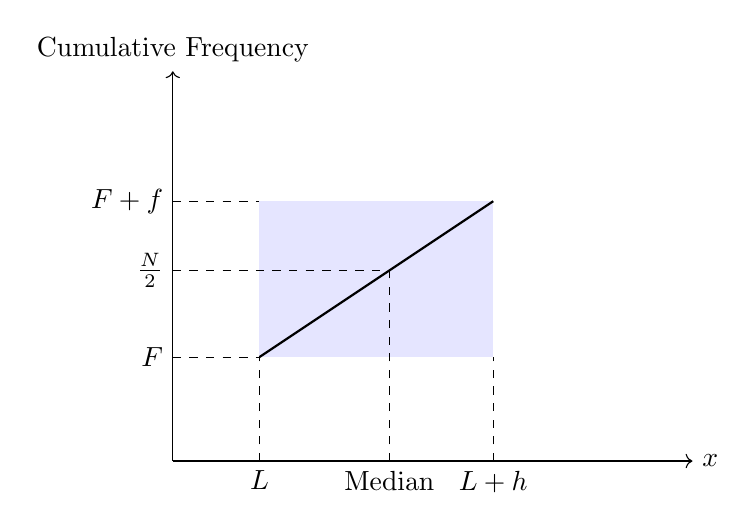
\begin{tikzpicture}[scale=1.1]
    % Axes
    \draw[->] (0,0) -- (6,0) node[right] {$x$};
    \draw[->] (0,0) -- (0,4.5) node[above] {Cumulative Frequency};

    % Median class block
    \fill[blue!10] (1,1.2) rectangle (3.7,3);

    % Horizontal lines
    \draw[thick] (1,1.2) -- (3.7,3);

    % Vertical dashed line for N/2
    \draw[dashed] (2.5,0) -- (2.5,2.2);
    \node[below] at (2.5,0) {Median};

    % Horizontal dashed to line
    \draw[dashed] (0,2.2) -- (2.5,2.2);
    \node[left] at (0,2.2) {$\frac{N}{2}$};

    % Horizontal frequency lines
    \draw[dashed] (0,1.2) -- (1,1.2);
    \draw[dashed] (0,3) -- (1,3);
    \node[left] at (0,1.2) {$F$};
    \node[left] at (0,3) {$F + f$};

    % Class boundaries
    \node[below] at (1,0) {$L$};
    \node[below] at (3.7,0) {$L + h$};
    \draw[dashed] (1,0) -- (1,1.2);
    \draw[dashed] (3.7,0) -- (3.7,1.2);

    % Brace for h
    % \draw[decorate,decoration={brace,mirror,amplitude=5pt},yshift=-5pt]
    %     (1,0) -- (4,0) node[midway,below,yshift=-6pt] {$h$};

    % Median label
    % \node[above] at (2.5,2.2) {\textbf{Median}};

\end{tikzpicture}
\end{center}

\textbf{Example}: Consider the following table containing the class values, frequencies and cumulative frequencies.


\begin{table}[H]
\begin{center}
\begin{tabular}{c|c|c}
	\toprule
	\textbf{Class Interval} & \textbf{Frequency} & \textbf{Cumulative Frequency} \\
	\midrule
	0--10 & 5 & 5\\
	10--20 & 8 & 13\\
	20--30 & 12 & 25\\
	30--40 & 6 & 31\\
	\bottomrule
\end{tabular}
\caption{\textit{Grouped frequency distribution table for calculating the median.}}
\end{center}
\end{table}

\[
N = 5 + 8 + 12 + 6 = 31,\quad \frac{N}{2} = 15.5
\]

Since $15.5$ is in between 13 and 25, the Median class is 20--30. Thus,
$$L = 20, F = 13, f = 12, h = 10$$

\[
\text{Median} = 20 + \left( \frac{15.5 - 13}{12} \right) \cdot 10 = 20 + \left( \frac{2.5}{12} \right) \cdot 10 = 20 + 2.08 = 22.08
\]
\end{enumerate}

\begin{textbox}
\textbf{Theorem}: Let \( x_1, x_2, \ldots, x_n \) be a set of observations. Define the function:
\[
S(A) = \sum_{i=1}^n |x_i - A|
\]
Then \( S(A) \) is minimized when \( A = \text{Median} \).
\end{textbox}
\textbf{Proof}: Let us arrange the observations \( x_1, x_2, \ldots, x_n \) in increasing order and denote the ordered sequence by \( y_1, y_2, \ldots, y_n \). Since this is just a rearrangement of the original data, we have:
\[
\sum_{i=1}^n |x_i - A| = \sum_{i=1}^n |y_i - A|.
\]

We now analyze the behavior of this sum in two cases:

\begin{itemize}
    \item \textbf{Case 1: \( n \) is odd (say \( n = 2m + 1 \))}

    \begin{align*}
    \sum_{i=1}^{n} |x_i - A| &= \sum_{i=1}^{2m+1} |y_i - A| \\
    &= |y_1 - A| + |y_2 - A| + \cdots + |y_m - A| + |y_{m+1} - A| \\
    &\quad + |y_{m+2} - A| + \cdots + |y_{2m+1} - A|.
    \end{align*}

    There are \( 2m + 1 \) terms in the sum. We consider them in symmetric pairs from both ends:

    \begin{itemize}
        \item The sum \( |y_1 - A| + |y_{2m+1} - A| \) is minimized when \( A \in [y_1, y_{2m+1}] \).
        \item The sum \( |y_2 - A| + |y_{2m} - A| \) is minimized when \( A \in [y_2, y_{2m}] \).
        \item Continuing this way, the sum \( |y_m - A| + |y_{m+2} - A| \) is minimized when \( A \in [y_m, y_{m+2}] \).
    \end{itemize}

    The unpaired central term is \( |y_{m+1} - A| \), which attains its minimum value (zero) when \( A = y_{m+1} \).

    Since all these intervals of minimization overlap at \( y_{m+1} \), we conclude that:
    \[
    \sum_{i=1}^{n} |x_i - A| \text{ is minimized when } A = y_{m+1} = \text{Median}.
    \]

    \item \textbf{Case 2: \( n \) is even (say \( n = 2m \))}

    \begin{align*}
    \sum_{i=1}^{n} |x_i - A| &= \sum_{i=1}^{2m} |y_i - A| \\
    &= |y_1 - A| + |y_2 - A| + \cdots + |y_m - A| + |y_{m+1} - A| + \cdots + |y_{2m} - A|.
    \end{align*}

    Now there are \( 2m \) terms, which can be grouped into \( m \) symmetric pairs:

    \begin{itemize}
        \item \( |y_1 - A| + |y_{2m} - A| \) is minimized when \( A \in [y_1, y_{2m}] \),
        \item \( |y_2 - A| + |y_{2m-1} - A| \) is minimized when \( A \in [y_2, y_{2m-1}] \), and so on.
        \item The final pair \( |y_m - A| + |y_{m+1} - A| \) is minimized when \( A \in [y_m, y_{m+1}] \).
    \end{itemize}

    Thus, the entire sum is minimized when \( A \in [y_m, y_{m+1}] \). A natural choice is:
    \[
    A = \text{Median} = \frac{y_m + y_{m+1}}{2},
    \]
    which lies within the minimizing interval and hence ensures that the sum is minimized.
\end{itemize}

In both cases—odd and even number of observations—the value of \( A \) that minimizes \( \sum_{i=1}^{n} |x_i - A| \) is the \textbf{median} of the dataset.

    \hfill $\blacksquare$

\begin{textbox}
The median is a better measure of central tendency than the mean (AM) in the presence of outliers in the observations.
\end{textbox}

The \textbf{mean} (AM) is sensitive to extreme values or outliers, while the \textbf{median} (the middle value) is more robust and resistant to such anomalies. This makes the median a better measure of central tendency in the presence of outliers or skewed data.

Consider the marks obtained by 5 students:

\[
\text{Scores} = \{10, 70, 75, 80, 90\}
\]

\[\textbf{Mean} = \frac{70 + 75 + 80 + 85 + 90}{5} = \frac{400}{5} = 80; \quad \textbf{Median} = \text{Middle value} = 75
\]

Here, both the mean and the median are equal and representative of the data, as there are no extreme values.

Now suppose one student scored unusually low:
\[
\text{Scores} = \{10, 70, 75, 80, 90\}
\]

\[\textbf{Mean} = \frac{10 + 70 + 75 + 80 + 90}{5} = \frac{325}{5} = 65; \quad \textbf{Median} = \text{Middle value} = 75
\]

The mean drops to 65 due to the outlier (10), even though most students scored 70 or above. The median stays at 75 and gives a better picture of the typical student performance.

\subsection{Mode}
\begin{textbox}
The \textbf{mode} of a given set of observations is the value which occurs with maximum frequency. It represents the highest peak in the frequency distribution.
    \end{textbox}

The mode is generally denoted by \( M_o \).

\begin{enumerate}

\item \textbf{Mode in a Simple Series (Ungrouped Data)}

To determine the mode:
\begin{itemize}
    \item Count the frequency of each data value.
    \item The mode is the value with the highest frequency.
\end{itemize}

\textbf{Example:} Find the mode of the dataset:
\[
3, 7, 2, 3, 9, 3, 5
\]
The number 3 occurs most frequently (3 times), so:
\[
\text{Mode} = 3
\]

\item \textbf{Mode in a Simple Frequency Distribution}

In a simple frequency distribution, the mode is the data value corresponding to the maximum frequency.

\textbf{Example:} Consider the table:

\begin{table}[H]
\begin{center}
	\begin{tabular}{c|c}
		\toprule
		\textbf{Value} & \textbf{Frequency} \\
		\midrule
		4 & 3 \\
		5 & 7 \\
		6 & 5 \\
		7 & 2 \\
		\bottomrule
	\end{tabular}
\end{center}
\caption{\textit{Simple frequency distribution table for calculating mode.}}
\end{table}

The highest frequency is 7, corresponding to the value 5. Hence:
\[
\text{Mode} = 5
\]

\item \textbf{Mode in a Grouped Frequency Distribution}

When the data is grouped into intervals, it is very difficult to find the mode accurately. However if all the classes are of equal width, then it is possible to approximately calculate the mode using the formula:
\begin{textbox}
\[
\text{Mode} = L + \left( \frac{f_1 - f_0}{2f_1 - f_0 - f_2} \right) \cdot h
\]
    \end{textbox}

where:
\begin{itemize}
    \item \( L \): lower boundary of the modal class
    \item \( f_1 \): frequency of the modal class
    \item \( f_0 \): frequency of the class preceding the modal class
    \item \( f_2 \): frequency of the class succeeding the modal class
    \item \( h \): class width
\end{itemize}

How do we arrive at the formula for mode? In addition to the modal class frequency $f_1$, mode also depends on $f_0$ (the frequency of the class preceding the modal class) and $f_2$ (the frequency of the class following the modal class). If they are equal, then one would take the midpoint of the modal class $L+ \dfrac{h}{2}$ as the mode. However, if $f_0-f_1$ is greater (smaller) than $f_1-f_2$, then one would suppose that the mode is nearer to (further from) the lower boundary ($L$) of the modal class than the upper boundary ($L+h$). Mathematically, if we assume the proportion is same, then
\[
\frac{d}{f_1 - f_0} = \frac{h - d}{f_1 - f_2}
\]

Cross-multiplying and simplifying:
\[
d\cdot (2f_1 - f_0 - f_2) = (f_1 - f_0)\cdot h
\]

Solving for \( d \):
\[
d = \frac{(f_1 - f_0)\cdot h}{2f_1 - f_0 - f_2}
\]

Hence, the mode is:
\[
\text{Mode} = L + d = L + \left( \frac{f_1 - f_0}{2f_1 - f_0 - f_2} \right) \cdot h
\]

\begin{center}
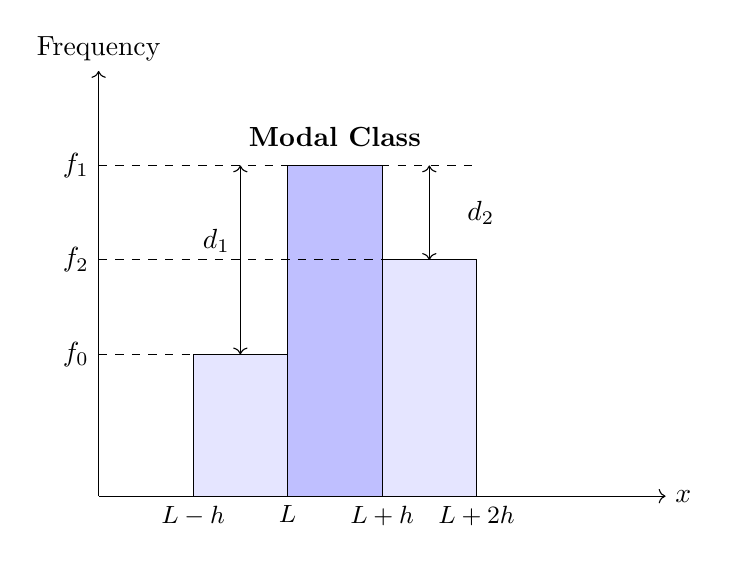
\begin{tikzpicture}[scale=1.2]

% Axes
\draw[->] (0,0) -- (6,0) node[right] {$x$};
\draw[->] (0,0) -- (0,4.5) node[above] {Frequency};

% Class boundaries
\draw[dashed] (1,0) -- (1,1.5);
\draw[dashed] (2,0) -- (2,3.5);
\draw[dashed] (3,0) -- (3,2.5);

% Frequency bars
\filldraw[fill=blue!10,draw=black] (1,0) rectangle (2,1.5); % f0
\filldraw[fill=blue!25,draw=black] (2,0) rectangle (3,3.5); % f1 modal class
\filldraw[fill=blue!10,draw=black] (3,0) rectangle (4,2.5); % f2

% Labels for class intervals
\node[below] at (1,0) {\small $L - h$};
\node[below] at (2,0) {\small $L$};
\node[below] at (3,0) {\small $L + h$};
\node[below] at (4,0) {\small $L + 2h$};

% Labels for frequencies
\node[left] at (0,1.5) {$f_0$};
\node[left] at (0,3.5) {$f_1$};
\node[left] at (0,2.5) {$f_2$};

% Dashed horizontal lines for f0, f1, f2
\draw[dashed] (0,1.5) -- (1,1.5);
\draw[dashed] (0,3.5) -- (4,3.5);
\draw[dashed] (0,2.5) -- (3,2.5);

% Modal class label
\node at (2.5,3.8) {\textbf{Modal Class}};

% Deltas
\draw[<->] (1.5,1.5) -- (1.5,3.5);
\node[right] at (1,2.7) {$d_1$};

\draw[<->] (3.5,2.5) -- (3.5,3.5);
\node[right] at (3.8,3.0) {$d_2$};
\end{tikzpicture}
\end{center}

\textbf{Example:} Consider the following grouped data:

\begin{table}[H]
\begin{center}
	\begin{tabular}{c|c}
		\toprule
		\textbf{Class Interval} & \textbf{Frequency} \\
		\midrule
		0--10 & 4 \\
		10--20 & 6 \\
		20--30 & 10 \\
		30--40 & 8 \\
		\bottomrule
	\end{tabular}
\end{center}
\caption{\textit{Grouped frequency distribution table for calculating the mode.}}
\end{table}

Here, the modal class is 20--30 because it has the highest frequency (\( f_1 = 10 \)). The required values are:
\[
L = 20, \quad f_0 = 6, \quad f_1 = 10, \quad f_2 = 8, \quad h = 10
\]

\[
\text{Mode} = 20 + \left( \frac{10 - 6}{2(10) - 6 - 8} \right) \cdot 10 = 20 + \left( \frac{4}{6} \right) \cdot 10 = 20 + 6.67 = 26.67
\]

\end{enumerate}


\subsection{Comparison and When to Use Each}

\begin{itemize}
    \item \textbf{Mean} is sensitive to outliers and skewed data. It is best used for symmetric, continuous data without extreme values.

    \item \textbf{Median} is more robust to outliers and skewed distributions. It is ideal when the data contain extreme values or are not symmetrically distributed.

    \item \textbf{Mode} is useful for categorical or discrete data, especially when identifying the most frequent category is of interest.

    \item \textbf{Geometric Mean} is appropriate when dealing with ratios, growth rates, or multiplicative processes (e.g., population growth, interest rates).

    \item \textbf{Harmonic Mean} is best for averaging rates, such as speed or price per unit when quantities vary.

\end{itemize}

Each measure gives a different perspective of the `center' of the data. The choice of measure should be guided by the nature and scale of the data, and the specific analysis objective.

\section{Partition Values: Quartiles, Deciles, and Percentiles}

Just as the median divides a data set into two equal parts, there are other statistical measures that partition the data into a fixed number of equal segments — such as 4, 10, or 100 parts when the data is arranged in increasing order of magnitude. These measures are collectively referred to as \textbf{partition values} or \textbf{quantiles}. The most commonly used partition values are the \textbf{quartiles}, \textbf{deciles}, and \textbf{percentiles}, which divide the data into four, ten, and one hundred equal parts, respectively.

Partition values are useful in identifying the spread and concentration of data. For instance, if a student scores at the 90th percentile, they performed better than 90\% of the population.

\subsection{Quartiles}

Quartiles divide a ordered data set into four equal parts. There are three quartiles:

\begin{itemize}
    \item $Q_1$ (First Quartile): 25\% of the data falls below $Q_1$.
    \item $Q_2$ (Second Quartile or Median): 50\% of the data falls below $Q_2$.
    \item $Q_3$ (Third Quartile): 75\% of the data falls below $Q_3$.
\end{itemize}

\begin{textbox}
\[
Q_k = \left( \frac{k(n+1)}{4} \right)\text{th value}, \quad k = 1, 2, 3
\]
\end{textbox}

% \textbf{Formula (for grouped data)}:
% \[
% Q_k = L + \left( \frac{\frac{kN}{4} - F}{f} \right) \cdot h
% \]
% where:
% \begin{itemize}
%     \item $L$ = lower boundary of the quartile class
%     \item $N$ = total frequency
%     \item $F$ = cumulative frequency before the quartile class
%     \item $f$ = frequency of the quartile class
%     \item $h$ = class width
% \end{itemize}

\textbf{Example}: Consider the ordered data: \{5, 7, 8, 12, 13, 15, 16, 20, 21\}.

\begin{itemize}
    \item Number of observations $ n = 9$
    \item $Q_1 = \left( \frac{1(9+1)}{4} \right) = \text{3rd value} = 8$
    \item $Q_2 = \left( \frac{2(9+1)}{4} \right) = \text{5th value} = 13$
    \item $Q_3 = \left( \frac{3(9+1)}{4} \right) = \text{7th value} = 16$
\end{itemize}

\textbf{Interquartile Range (IQR)}: The {Interquartile Range (IQR)} is a measure of statistical dispersion, which describes the spread of the middle 50\% of a data set. It is the difference between the third quartile (\(Q_3\)) and the first quartile (\(Q_1\)).

\begin{textbox}
    \[
    \text{IQR} = Q_3 - Q_1
    \]
\end{textbox}

\subsection{Deciles}

Deciles divide the ordered data into ten equal parts. There are nine deciles ($D_1$ to $D_9$), such that:

\begin{textbox}
\[
D_k = \left( \frac{k(n+1)}{10} \right)\text{th value}, \quad k = 1, 2, \dots, 9
\]
\end{textbox}

% \textbf{Grouped data formula}:
% \[
% D_k = L + \left( \frac{\frac{kN}{10} - F}{f} \right) \cdot h
% \]

\subsection{Percentiles}

Percentiles divide the ordered data into one hundred equal parts. There are 99 percentiles ($P_1$ to $P_{99}$), commonly used to interpret standardized test scores and similar metrics.

\begin{textbox}
\[
P_k = \left( \frac{k(n+1)}{100} \right)\text{th value}, \quad k = 1, 2, \dots, 99
\]
\end{textbox}

% \textbf{Grouped data formula}:
% \[
% P_k = L + \left( \frac{\frac{kN}{100} - F}{f} \right) \cdot h
% \]

\section{Measures of Dispersion}

Measures of dispersion describe the spread or variability within a data set. While measures of central tendency (such as the mean or median) indicate the typical value, measures of dispersion indicate how much the values in the dataset differ from the central value. A small dispersion means the data points are clustered close to the center, while a large dispersion indicates data points are spread out over a wide range.

Consider the following two data sets, each containing five values:
$A = \{4, 5, 5, 5, 6\}$ and $B = \{1, 3, 5, 7, 9\}$.
Both sets have the same mean, which is 5. For set $A$, the mean is
\[
\frac{4 + 5 + 5 + 5 + 6}{5} = \frac{25}{5} = 5,
\]
and for $B$, the mean is
\[
\frac{1 + 3 + 5 + 7 + 9}{5} = \frac{25}{5} = 5.
\]
However, their dispersions are quite different. The maximum value of $A$ is $6$ and minimum value is $4$, whereas the maximum value of $B$ is $9$ and minimum value is $1$. This means that although both sets center around the same average value, the values in set $B$ are spread out much more widely around the mean compared to set $A$. Therefore, we say that the dispersion of $B$ is greater than that of $A$.


Measures of dispersion are broadly classified into two types:
\begin{itemize}
    \item \textbf{Absolute Measures of Dispersion}: These express dispersion in the same units as the original data.
    \item \textbf{Relative Measures of Dispersion}: These express dispersion as a ratio or percentage and are unit-free. They are useful for comparing variability between datasets with different units or magnitudes.
\end{itemize}

\begin{center}
    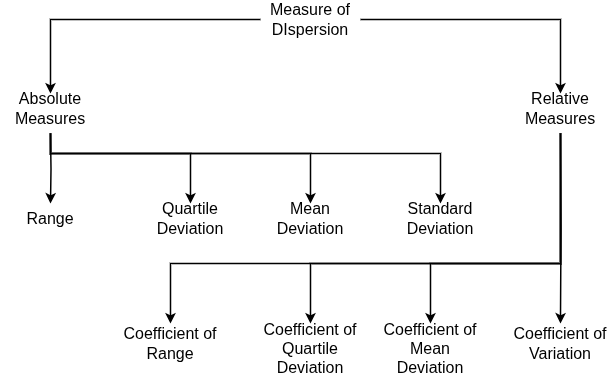
\includegraphics[scale=0.5]{pic/mod.drawio.png}
\end{center}

\subsection{Absolute Measures of Dispersion}

\begin{enumerate}
    \item \textbf{Range}: Difference between the largest and smallest observations.
    \begin{textbox}
        \[
    \text{Range} = L - S
    \]
    \end{textbox}
    where \( L \) is the largest value and \( S \) is the smallest value.

    Consider the data set: \{10, 15, 18, 22, 25\}.
Here, the largest value \( L = 25 \) and the smallest value \( S = 10 \).

\[
\text{Range} = 25 - 10 = 15
\]
    \item \textbf{Quartile Deviation (Semi-Interquartile Range)}: Quartile deviation is defined as half the difference between the lower and upper quartiles.
    \begin{textbox}
    \[
    \text{Quartile Deviation} = \frac{Q_3 - Q_1}{2}
    \]
    \end{textbox}
    where \( Q_1 \) and \( Q_3 \) are the first and third quartiles.

    Consider the ordered data set: \{10, 15, 20, 25, 30, 35, 40\}.

Here,
\[
Q_1 = 15, \quad Q_3 = 35
\]

\[
\text{Quartile Deviation} = \frac{35 - 15}{2} = \frac{20}{2} = 10
\]

    \item \textbf{Mean Deviation}: Mean deviation is the arithmetic mean of absolute deviations from mean or any other specified value.
    \begin{textbox}
    \[
    \text{Mean Deviation about }A = \frac{1}{n} \sum_{i=1}^{n} |x_i - A|
    \]
    \end{textbox}
    Generally mean deviation is taken from the arithmetic mean $\overline{x}$.
    \begin{textbox}
    \[
    \text{Mean Deviation about mean} = \frac{1}{n} \sum_{i=1}^{n} |x_i - A|
    \]
    \end{textbox}

    Consider the data set: \{2, 4, 6, 8, 10\}. First we calculate the mean from the data:
\[
\overline{x} = \frac{2 + 4 + 6 + 8 + 10}{5} = \frac{30}{5} = 6
\]

Then we compute the absolute deviations from the mean:
\[
|2 - 6| = 4,\quad |4 - 6| = 2,\quad |6 - 6| = 0,\quad |8 - 6| = 2,\quad |10 - 6| = 4
\]

Finally we calculate the Mean Deviation about the mean:
\[
\text{Mean Deviation about mean} = \frac{4 + 2 + 0 + 2 + 4}{5} = \frac{12}{5} = 2.4
\]

For weighted data, the Mean Deviation about the mean is given by:

\begin{textbox}
\[
\text{Mean Deviation about mean} = \frac{\sum_{i=1}^{n} f_i \left| x_i - \overline{x} \right|}{\sum_{i=1}^{n} f_i}
\]
\end{textbox}

where:
\begin{itemize}
    \item \( x_i \) are the data values,
    \item \( f_i \) are their corresponding frequencies (weights),
    \item \( \overline{x} = \dfrac{\sum_i f_i x_i}{\sum_i f_i} \) is the weighted mean.
\end{itemize}

    \item \textbf{Standard Deviation}: In considering the deviations $x_i-A$ for obtaining a measure of dispersion, we may also get rid of their signs by taking their squares $(x_i-A)^2$, instead of taking their absolute values $|x_i-A|$. The square root of the arithmetic mean of these squares i.e. $\sqrt{\dfrac{1}{n}\sum_{i=1}^n(x_i-A)^2}$ which is called the \textbf{root mean square deviation} about $A$, may be accepted as a measure of dispersion. When $A=\overline{x}$, the measure of dispersion is called the standard deviation.
    \begin{textbox}
    \[
    \text{Standard deviation} = \sigma = \sqrt{\frac{1}{n} \sum_{i=1}^{n} (x_i - \overline{x})^2}
    \]
    \end{textbox}
    The square of the standard deviation i.e. $\sigma^2$ is known as \textbf{variance}.

    As an example, consider the data set: \{2, 4, 4, 4, 5, 5, 7, 9\}. First we calculate the mean:
\[
\overline{x} = \frac{2 + 4 + 4 + 4 + 5 + 5 + 7 + 9}{8} = \frac{40}{8} = 5
\]

Then we find the Squared Deviations from the mean:
\[
(2 - 5)^2 = 9,\quad (4 - 5)^2 = 1,\quad (4 - 5)^2 = 1,\quad (4 - 5)^2 = 1,
\]
\[
(5 - 5)^2 = 0,\quad (5 - 5)^2 = 0,\quad (7 - 5)^2 = 4,\quad (9 - 5)^2 = 16
\]

Finally compute the Standard Deviation:
\[
\sigma = \sqrt{\frac{9 + 1 + 1 + 1 + 0 + 0 + 4 + 16}{8}} = \sqrt{\frac{32}{8}} = \sqrt{4} = 2
\]

For weighted data, the standard deviation is calculated as:

\begin{textbox}
\[
\text{Standard deviation} = \sigma = \sqrt{\frac{\sum_{i=1}^n f_i (x_i - \overline{x})^2}{\sum_{i=1}^n f_i}}
\]
\end{textbox}

where,
\begin{itemize}
    \item \(x_i\) are the data values,
    \item \(f_i\) are the corresponding frequencies (weights),
    \item \(\overline{x} = \dfrac{\sum_{i=1}^n f_i x_i}{\sum_{i=1}^n f_i}\) is the weighted mean,
\end{itemize}

\begin{textbox}
\textbf{Theorem}: If \( x = a \) (a constant), {then } \( \sigma_x = 0 \).
\end{textbox}

\textbf{Proof}: Since all observations are equal to \( a \), the mean is
\[
\overline{x} = a.
\]
The standard deviation is
\begin{align*}
\sigma_x &= \sqrt{\frac{1}{n} \sum_{i=1}^n (x_i - \overline{x})^2} = \sqrt{\frac{1}{n} \sum_{i=1}^n (a - a)^2} = \sqrt{0} = 0.
\end{align*}

\hfill $\blacksquare$

\begin{textbox}
\textbf{Theorem}: If \( y = a + b x \), {where} \( a, b \) {are constants, then}
\[
\sigma_y = |b| \sigma_x
\]
\end{textbox}

\textbf{Proof}: The mean of \( y \) is
\[
\overline{y} = a + b \overline{x}
\]
The standard deviation of \( y \) is
\begin{align*}
\sigma_y &= \sqrt{\frac{1}{n} \sum_{i=1}^n (y_i - \overline{y})^2} = \sqrt{\frac{1}{n} \sum_{i=1}^n (a + b x_i - (a + b \overline{x}))^2} \\
         &= \sqrt{\frac{1}{n} \sum_{i=1}^n \left(b (x_i - \overline{x})\right)^2} = \sqrt{\frac{1}{n} \sum_{i=1}^n b^2 (x_i - \overline{x})^2} \\
         &= |b| \sqrt{\frac{1}{n} \sum_{i=1}^n (x_i - \overline{x})^2} = |b| \sigma_x
\end{align*}

\hfill $\blacksquare$

\begin{textbox}
\textbf{Theorem (Pooled standard deviation)}: Let a dataset be composed of two groups:

\begin{itemize}
  \item Group 1: \( n_1 \) observations, mean \( \overline{x}_1 \), standard deviation \( \sigma_1 \),
  \item Group 2: \( n_2 \) observations, mean \( \overline{x}_2 \), standard deviation \( \sigma_2 \).
\end{itemize}

{Then the combined (pooled) standard deviation \( \sigma \) of the dataset (size \( n = n_1 + n_2 \)) is given by:}

\[
\sigma = \sqrt{
\frac{n_1 \sigma_1^2 + n_2 \sigma_2^2}{n_1 + n_2} + \frac{n_1 (\overline{x}_1 - \overline{x})^2 + n_2 (\overline{x}_2 - \overline{x})^2}{n_1 + n_2}
}
\]
where
\[
\overline{x} = \frac{n_1 \overline{x}_1 + n_2 \overline{x}_2}{n_1 + n_2}
\]
\end{textbox}

\textbf{Proof}: Let us denote $x_{1j}, (j=1,2,\dots, n_1)$ and $x_{2j}, (j=1,2,\dots, n_1)$ the values of the two sets. Then
$$\sigma_1^2 =\sum_{j=1}^{n_1} (x_{1j} - \overline{x}_1), \quad \sigma_2^2 =\sum_{j=1}^{n_1} (x_{2j} - \overline{x}_2)$$


The variance of the combined data set is
\begin{align*}
\sigma^2 &= \frac{1}{n_1 + n_2} \left(\sum_{j=1}^{n_1} (x_{1j} - \overline{x})^2 + \sum_{j=1}^{n_2} (x_{2j} - \overline{x})^2 \right)
\end{align*}

Expanding the first term:
\begin{align*}
\sum_{j=1}^{n_1} (x_{ij} - \overline{x})^2 &= \sum_{j=1}^{n_1} \left[(x_{1j} - \overline{x}_1) + (\overline{x}_1 - \overline{x})\right]^2 \\
&= \underbrace{\sum_{j=1}^{n_1} (x_{1j} - \overline{x}_1)^2}_{= n_1\sigma_1^2} + 2(\overline{x}_1 - \overline{x}) \underbrace{\sum_{j=1}^{n_1} (x_{1j} - \overline{x}_1)}_{= 0} + \sum_{j=1}^{n_1} (\overline{x}_1 - \overline{x})^2 \\
&= n_1 \sigma_1^2 + n_1 (\overline{x}_1 - \overline{x})^2,
\end{align*}
Similarly,
\[
\sum_{j=1}^{n_2} (x_{2j} - \overline{x})^2 = n_2 \sigma_2^2 + n_2 (\overline{x}_2 - \overline{x})^2.
\]

Thus,
\begin{align*}
\sigma^2 &= \frac{n_1 \sigma_1^2 + n_2 \sigma_2^2}{n_1 + n_2} + \frac{n_1 (\overline{x}_1 - \overline{x})^2 + n_2 (\overline{x}_2 - \overline{x})^2}{n_1 + n_2}
\end{align*}

\hfill $\blacksquare$

\end{enumerate}

\subsection{Relative Measures of Dispersion}

Relative measures of dispersion are defined as ratio of absolute measures of dispersion to the corresponding measure of central tendency. The ratio is expressed in terms of a percentage.

\begin{enumerate}
    \item \textbf{Coefficient of Range}:
    \begin{textbox}
    \[
    \text{Coefficient of Range} = \frac{L - S}{L + S}\times 100\%
    \]
    \end{textbox}
    where \( L \) is the largest value and \( S \) is the smallest value.

    \item \textbf{Coefficient of Quartile Deviation}:
    \begin{textbox}
    \[
    \text{Coefficient of Q.D.} = \frac{Q_3 - Q_1}{Q_3 + Q_1}\times 100\%
    \]
    \end{textbox}

    \item \textbf{Coefficient of Mean Deviation}:
    \begin{textbox}
    \[
    \text{Coefficient of M.D.} = \frac{\text{Mean Deviation}}{\overline{x}}\times 100\%
    \]
    \end{textbox}

    \item \textbf{Coefficient of Variation (CV)}:
    \begin{textbox}
    \[
    \text{CV} = \frac{\sigma}{\overline{x}} \times 100\%
    \]
    \end{textbox}
\end{enumerate}

\section{Moments, Skewness and Kurtosis}

\subsection{Raw Moments and Central Moments}

In descriptive statistics, \textbf{moments} are used to describe various characteristics of a dataset's distribution. Two important types of moments are:

\begin{itemize}
    \item \textbf{Raw moments} (moments about the origin): The $r$-th \textbf{raw moment} of a dataset $x_1, x_2, \dots, x_n$ is given by:
\begin{textbox}
\[
\mu'_r = \frac{1}{n} \sum_{i=1}^{n} x_i^r
\]
\end{textbox}
    \begin{itemize}
        \item First raw moment: $\mu'_1 = \overline{x}$ (sample mean)
        \item Second raw moment: $\mu'_2 = \frac{1}{n} \sum x_i^2$
    \end{itemize}
    \item \textbf{Central moments} (moments about the mean): The $r$-th \textbf{central moment} is the average of the $r$-th powers of deviations from the mean:
\begin{textbox}
\[
\mu_r = \frac{1}{n} \sum_{i=1}^{n} (x_i - \overline{x})^r
\]
\end{textbox}
\begin{itemize}
    \item First central moment: $\mu_1 = 0$ (since the mean deviation is zero)
    \item Second central moment: $\mu_2 = \dfrac{1}{n} \sum_{i=1}^{n} (x_i - \overline{x})^2$ is the {variance}.
\end{itemize}
\end{itemize}

\textbf{Example}: Consider the dataset:
\[
\{2,\ 4,\ 6,\ 8\}
\]
\begin{itemize}
\item{Raw moments:}
\begin{align*}
\mu'_1 &= \frac{1}{4}(2 + 4 + 6 + 8) = 5 \\
\mu'_2 &= \frac{1}{4}(2^2 + 4^2 + 6^2 + 8^2) = \frac{120}{4} = 30
\end{align*}

\item{Central moments:}
\begin{align*}
\mu_1 &= 0\\
\mu_2 &= \frac{1}{4}[(2 - 5)^2 + (4 - 5)^2 + (6 - 5)^2 + (8 - 5)^2] \\
      &= \frac{1}{4}(9 + 1 + 1 + 9) = \frac{20}{4} = 5
% \mu_3 &= \frac{1}{4}[(2 - 5)^3 + (4 - 5)^3 + (6 - 5)^3 + (8 - 5)^3] \\
%       &= \frac{1}{4}[-27 - 1 + 1 + 27] = 0
\end{align*}

\end{itemize}

\subsection{Relationship Between Raw and Central Moments}

The $r$-th central moment $\mu_r$ can be expressed in terms of raw moments $\mu'_k$ and powers of the mean $\overline{x}$:

\begin{align*}
    \mu_r &= \frac{1}{n} \sum_{i=1}^n (x_i - \overline{x})^r = \frac{1}{n}\sum_{i=1}\left[\sum_{k=0}^r \binom{r}{k}\,\overline{x_i}^{\,r-k} \overline{x}^k\right]\\
    &=\frac{1}{n}\sum_{i=1}^n\left[x_i^r - \binom{r}{1} x_i^{r-1}\overline{x} + \binom{r}{2} x_i^{r-2}\overline{x}^2 + \dots - \overline{x}^r\right]\\
    &=\mu'_r - \binom{r}{1} \mu'_{r-1}\overline{x} + \binom{r}{2} \mu'_{r-2}\overline{x}^2 + \dots - n\overline{x}^r
\end{align*}

Since $\mu'_1 = \overline{x}$, we can rewrite the above expression as:
\begin{textbox}
$$\mu_r = \mu'_r - \binom{r}{1} \mu'_{r-1}\mu'_1 + \binom{r}{2} \mu'_{r-2}{\mu'_1}^2 + \dots - n{\mu'_1}^r$$
\end{textbox}
% Now putting $r = 1,2,3,4$, we get

\begin{itemize}
  \item \(r=1:\)
    \begin{align*}
      \mu_1
      &= \mu'_1 - \binom{1}{1}\,\mu'_0\,\mu'_1 \\
      &= \mu'_1 - \mu'_1 = 0
    \end{align*}


  \item \(r=2:\)
    \begin{align*}
      \mu_2
      &= \mu'_2
         - \binom{2}{1}\,\mu'_1\,\mu'_1
         + \binom{2}{2}\,\mu'_0\,(\mu'_1)^2 \\
      &= \mu'_2 - 2(\mu'_1)^2 + (\mu'_1)^2
      = \mu'_2 - (\mu'_1)^2
    \end{align*}


  \item \(r=3:\)
    \begin{align*}
      \mu_3
      &= \mu'_3
         - \binom{3}{1}\,\mu'_2\,\mu'_1
         + \binom{3}{2}\,\mu'_1\,(\mu'_1)^2
         - \binom{3}{3}\,\mu'_0\,(\mu'_1)^3 \\
      &= \mu'_3 - 3\,\mu'_2\,\mu'_1 + 3(\mu'_1)^3 - (\mu'_1)^3
      = \mu'_3 - 3\,\mu'_2\,\mu'_1 + 2(\mu'_1)^3
    \end{align*}


  \item \(r=4:\)
    \begin{align*}
      \mu_4
      &= \mu'_4
         - \binom{4}{1}\,\mu'_3\,\mu'_1
         + \binom{4}{2}\,\mu'_2\,(\mu'_1)^2
         - \binom{4}{3}\,\mu'_1\,(\mu'_1)^3
         + \binom{4}{4}\,\mu'_0\,(\mu'_1)^4 \\
      &= \mu'_4 - 4\,\mu'_3\,\mu'_1 + 6\,\mu'_2\,(\mu'_1)^2 - 4(\mu'_1)^4 + (\mu'_1)^4 \\
      &= \mu'_4 - 4\,\mu'_3\,\mu'_1 + 6\,\mu'_2\,(\mu'_1)^2 - 3(\mu'_1)^4
    \end{align*}

\end{itemize}

Now let's derive the inverse relationship. Using the binomial expansion on \(x_i = (x_i - \overline{x}) + \overline{x}\), the \(r\)-th raw moment can be written as
\begin{align*}
\mu'_r
&= \frac{1}{n}\sum_{i=1}^n \bigl[\overline{x}+ (x_i - \overline{x})\bigr]^r
= \frac{1}{n}\sum_{i=1}^n\left[\sum_{k=0}^r \binom{r}{k}\,\overline{x}^{\,r-k} (x_i - \overline{x})^k\right]\\
&= \frac{1}{n}\sum_{i=1}^n\left[\overline{x}^r\
+ \binom{r}{1}\,\overline{x}^{\,r-1}\,(x_i - \overline{x})
+ \binom{r}{2}\,\overline{x}^{\,r-2}\,(x_i - \overline{x})^2
+ \cdots
+ (x_i - \overline{x})^r\right]\\
&= \overline{x}^r\
+ \binom{r}{1}\,\overline{x}^{\,r-1}\,\mu_1
+ \binom{r}{2}\,\overline{x}^{\,r-2}\,\mu_2
+ \cdots
+ \mu_r
\end{align*}
where by convention \(\mu_1 = 0\).

\begin{textbox}
    \begin{align*}
        \mu'_r = \overline{x}^r\
+ \binom{r}{1}\,\overline{x}^{\,r-1}\,\mu_1
+ \binom{r}{2}\,\overline{x}^{\,r-2}\,\mu_2
+ \cdots
+ \mu_r
    \end{align*}
\end{textbox}

\begin{itemize}
  \item \(r=1:\)
    \begin{align*}
      \mu'_1
      &= \overline{x}^1\ + \binom{1}{1}\,\overline{x}^0\,\mu_1 \\
      &= \overline{x} + 0
      = \overline{x}
    \end{align*}

  \item \(r=2:\)
    \begin{align*}
      \mu'_2
      &= \overline{x}^2\
         + \binom{2}{1}\,\overline{x}^1\,\mu_1
         + \binom{2}{2}\,\overline{x}^0\,\mu_2 \\
      &= \overline{x}^2 + 0 + \mu_2
      = \mu_2 + \overline{x}^2
    \end{align*}

  \item \(r=3:\)
    \begin{align*}
      \mu'_3
      &= \overline{x}^3\
         + \binom{3}{1}\,\overline{x}^2\,\mu_1
         + \binom{3}{2}\,\overline{x}^1\,\mu_2
         + \binom{3}{3}\,\overline{x}^0\,\mu_3 \\
      &= \overline{x}^3 + 0 + 3\,\overline{x}\,\mu_2 + \mu_3
      = \mu_3 + 3\,\overline{x}\,\mu_2 + \overline{x}^3
    \end{align*}

  \item \(r=4:\)

    \begin{align*}
      \mu'_4
      &= \overline{x}^4\
         + \binom{4}{1}\,\overline{x}^3\,\mu_1
         + \binom{4}{2}\,\overline{x}^2\,\mu_2
         + \binom{4}{3}\,\overline{x}^1\,\mu_3
         + \binom{4}{4}\,\overline{x}^0\,\mu_4 \\
      &= \overline{x}^4 + 0 + 6\,\overline{x}^2\,\mu_2 + 4\,\overline{x}\,\mu_3 + \mu_4 \\
      &= \mu_4 + 4\,\overline{x}\,\mu_3 + 6\,\overline{x}^2\,\mu_2 + \overline{x}^4
    \end{align*}
\end{itemize}

\subsection{Skewness}

\textbf{Skewness} is a measure of the asymmetry of a frequency distribution about its mean. The frequency distribution of a dataset is called symmetrical about the value $x_0$ if the frequency of $x_0-h$ is same as the frequency of $x_0+h$, whatever $h$ may be.


The sample skewness is defined as:
\begin{textbox}
\[
\text{Skewness} (\gamma_1) = \frac{1}{n} \sum_{i=1}^n \left( \frac{x_i - \overline{x}}{\sigma} \right)^3 = \frac{\mu_3}{\sigma^3}
\]
\end{textbox}
where \(\mu_3 = \dfrac{1}{n} \sum_{i=1}^n (x_i - \overline{x})^3\) is the third central moment.

The value of skewness determines the shape of the frequency curve:
\begin{itemize}
    \item If skewness \( = 0 \), the distribution is \textbf{symmetric}.
    \item If skewness \( > 0 \), the distribution is \textbf{positively skewed} (long right tail).
    \item If skewness \( < 0 \), the distribution is \textbf{negatively skewed} (long left tail).
\end{itemize}

\textbf{How to interpret the formula?}

Skewness uses cubed deviations $(x_i - \overline{x})^3$. Cubing serves two purposes: it preserves the sign of the deviation — meaning values greater than the mean contribute positively and those less than the mean contribute negatively — and it exaggerates the impact of larger deviations, making the measure sensitive to extreme values in the tails. This helps identify whether the data are stretched more to the right or left.

Dividing by the cube of the standard deviation $\sigma^3$ standardizes the measure, removing units and allowing for meaningful comparisons across datasets with different scales. The result is a dimensionless quantity: positive skewness indicates a long right tail, negative skewness signals a long left tail, and zero skewness implies symmetry around the mean.

\begin{center}
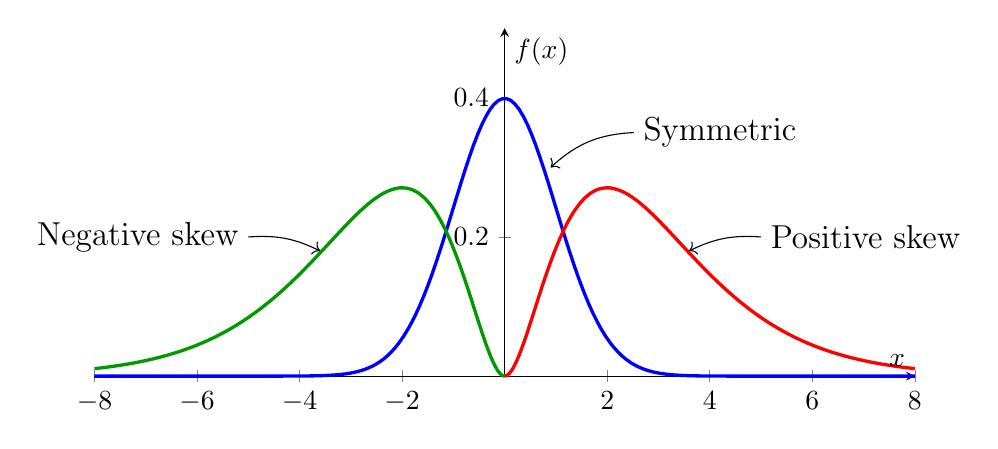
\begin{tikzpicture}
  \begin{axis}[
    width=12cm, height=6cm,
    axis lines=middle,
    ymin=0, ymax=0.5,
    xlabel={$x$}, ylabel={$f(x)$},
    domain=-8:8, samples=200,
    every axis plot post/.append style={very thick},
    clip=false            % allow arrows/nodes outside the plot area
  ]
    % Symmetric (Normal)
    \addplot[blue, very thick] {1/sqrt(2*pi)*exp(-x^2/2)};
    % Node and arrow for symmetric
    \node[black, font=\large] (sym) at (axis cs:4.2,0.35) {Symmetric};
    \draw[->, black] (sym.west) to[bend right=20] (axis cs:0.9,0.3);

    % Positive skew (Gamma shape)
    \addplot[red, thick, domain=0:8] {x^2*exp(-x)/2};
    % Node and arrow for positive skew
    \node[black, font=\large, right] (pos) at (axis cs:5,0.2) {Positive skew};
    \draw[->, black] (pos.west) to[bend right=15] (axis cs:3.6,0.18);

    % Negative skew (Reflected Gamma)
    \addplot[green!60!black, very thick, domain=-8:0] {(-x)^2*exp(x)/2};
    % Node and arrow for negative skew
    \node[black, font=\large, left] (neg) at (axis cs:-5,0.2) {Negative skew};
    \draw[->, black] (neg.east) to[bend left=15] (axis cs:-3.6,0.18);
  \end{axis}
\end{tikzpicture}
\end{center}


\textbf{Example}: Given data: \(x = \{2, 3, 4, 5, 8\}\)

\begin{itemize}
    \item Mean: \(\overline{x} = \dfrac{2+3+4+5+8}{5} = 4.4\)
    \item Standard deviation: \(s = \sqrt{\dfrac{1}{5}\sum_i (x_i - \overline{x})^2} \approx 2.058\)
    \item Third central moment:
    \[
    \mu_3 = \dfrac{1}{5} \left[(-2.4)^3 + (-1.4)^3 + (-0.4)^3 + 0.6^3 + 3.6^3\right] \approx 3.232
    \]
    \item Skewness:
    \[
    \gamma_1 = \frac{3.232}{(2.058)^3} \approx 0.37
    \]
\end{itemize}

Since skewness \(> 0\), the distribution is \textbf{positively skewed}.


In most unimodal distributions\footnote{A dataset is said to have a \textbf{unimodal distribution} if its values tend to cluster around a single (not multiple) central peak when plotted as a histogram or a frequency curve.}, the following ``rule of thumb'' holds regarding the ordering of Mean, Median, and Mode under skewness:

\begin{itemize}
  \item \textbf{Positive skew (right‐tailed):}
    \[
      \text{Mode} \;<\; \text{Median} \;<\; \text{Mean}.
    \]
    \\
    Extreme values on the right pull the mean farther out than the median, while the mode remains at the peak of the bulk of the data.

  \item \textbf{Negative skew (left‐tailed):}
    \[
      \text{Mean} \;<\; \text{Median} \;<\; \text{Mode}.
    \]
    \\
    Extreme values on the left drag the mean below the median, and the mode stays at the highest‐density point on the right.
\end{itemize}

\subsection{Kurtosis}

\textbf{Kurtosis} measures the degree of `peakedness' of a frequency distribution curve. Two frequency distributions may have the same mean, dispersion, and skewness, yet differ in how concentrated the values are around the mode. One distribution may have a sharper peak due to a higher concentration of values near the center, while the other appears flatter. This characteristic of a frequency distribution is known as kurtosis. It is calculated and reported either as an absolute or as a relative value. The absolute kurtosis is always a positive number.

\begin{textbox}
\[
\text{Absolute Kurtosis} \;=\;\frac{\mu_4}{\sigma^4}
\]
\end{textbox}
where \(\mu_4 = \dfrac{1}{n} \sum_{i=1}^n (x_i - \overline{x})^4\) is the fourth central moment.

The absolute kurtosis of a normal distribution, which we will learn in later chapter, is 3. The value 3 is taken as a datum (reference point) to calculate the relative kurtosis.
\begin{textbox}
\[
\text{Absolute Kurtosis}(\gamma_2) \;=\;\text{Relative Kurtosis} - 3
\]
\end{textbox}

\begin{itemize}
  \item Relative kurtosis \(=0\): \textbf{Mesokurtic} (e.g.\ Normal).
  \item Relative kurtosis \(>0\): \textbf{Leptokurtic} (heavy tails, sharp peak).
  \item Relative kurtosis \(<0\): \textbf{Platykurtic} (light tails, flat top).
\end{itemize}

\begin{center}
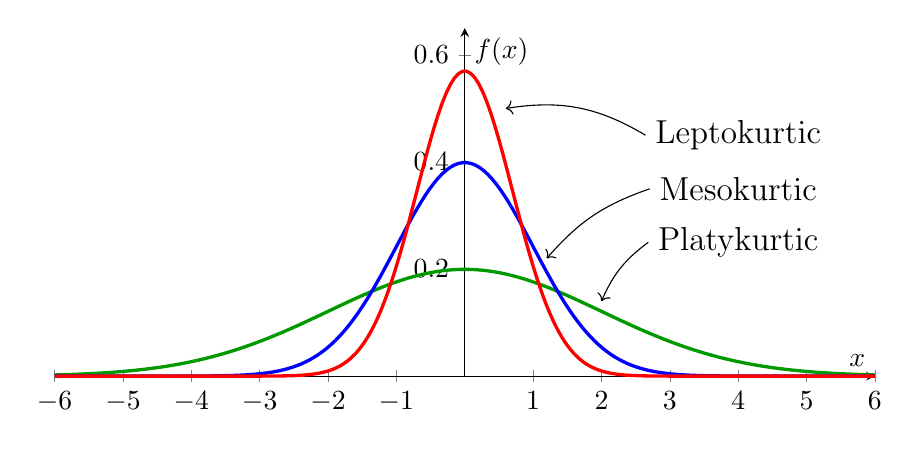
\begin{tikzpicture}
  \begin{axis}[
    width=12cm, height=6cm,
    axis lines=middle,
    ymin=0, ymax=0.65,
    xlabel={$x$}, ylabel={$f(x)$},
    domain=-6:6, samples=200,
    clip=false,
    every axis plot post/.append style={very thick},
  ]
    % Platykurtic: wider Gaussian (σ=2)
    \addplot[green!60!black] {1/(2*sqrt(2*pi)) * exp(-x^2/(2*2^2))};
    \node[black,font=\large] (platy) at (axis cs:4,0.25) {Platykurtic};
    \draw[->, black] (platy.west) to[bend right=15] (axis cs:2,0.14);

    % Mesokurtic: standard normal (σ=1)
    \addplot[blue] {1/sqrt(2*pi) * exp(-x^2/2)};
    \node[black,font=\large] (meso) at (axis cs:4,0.35) {Mesokurtic};
    \draw[->, black] (meso.west) to[bend right=15] (axis cs:1.2,0.22);

    % Leptokurtic: narrower Gaussian (σ=0.7)
    \addplot[red] {1/(0.7*sqrt(2*pi)) * exp(-x^2/(2*0.7^2))};
    \node[black,font=\large] (lepto) at (axis cs:4,0.45) {Leptokurtic};
    \draw[->, black] (lepto.west) to[bend right=20] (axis cs:0.6,0.5);
  \end{axis}
\end{tikzpicture}
\end{center}


\textbf{How to interpret the formula?}

Kurtosis raises deviations from the mean to the fourth power. This has a distinct purpose: it emphasizes extreme values far from the mean far more than values closer to it. Unlike cubing (used in skewness), which preserves the sign of deviations to detect asymmetry, raising to the fourth power removes the sign, treating all deviations equally, but magnifying larger ones disproportionately.

Before applying the fourth power, each deviation is \textbf{first divided by the standard deviation} $\sigma$. This step is crucial: it standardizes the scale of deviations, ensuring that the measure reflects the \textit{relative extremity} of values, not just their raw magnitude. Even if two distributions seem to have similar tail weights, the distribution with a \textit{smaller standard deviation} (i.e., a tighter central cluster) will yield \textit{larger standardized deviations}, which get exaggerated further by the fourth power.

Also, dividing the fourth central moment by $\sigma^4$ makes kurtosis a \textbf{dimensionless} and \textbf{scale-invariant} quantity, allowing meaningful comparisons across datasets.



\textbf{Example}: Using the same data \(x = \{2,3,4,5,8\}\):
\begin{itemize}
  \item Mean \(\overline{x}=4.4\), \quad Standard deviation \(\sigma\approx2.058\).
  \item Fourth central moment:
    \[
    \mu_4 = \frac{1}{5}\bigl[(-2.4)^4 + (-1.4)^4 + (-0.4)^4 + 0.6^4 + 3.6^4\bigr]
           \approx 41.03.
    \]
  \item \(\displaystyle \text{Kurtosis} (\gamma_2) = \frac{41.03}{(2.058)^4}\approx 2.29,\)
        \(\text{Relative Kurtosis}\approx -0.71\).
        This dataset is \textbf{platykurtic}.
\end{itemize}


\chapter{Theory of Probability}
\section{Some Notation and Terminology}
\subsection{Random Experiment}

An \textbf{experiment} is generally defined as one or more actions that result in a specific outcome.

\begin{textbox}
An experiment $E$ is called a \textbf{random experiment} if it satisfies the following conditions:

\begin{itemize}
    \item All possible outcomes of $E$ are known in advance.
    \item It is not possible to predict with certainty which specific outcome will occur in any given trial\footnote{A \textbf{trial} is a single performance or execution of an experiment. Tossing a coin once is a trial of the coin-tossing experiment.} of $E$.
    \item The experiment $E$ can be repeated, at least conceptually, under identical conditions an infinite number of times.
\end{itemize}
\end{textbox}

A common example of a random experiment is the tossing of a coin. The possible outcomes—`Head' and `Tail'—are known in advance, but it is impossible to determine with certainty which of the two outcomes will occur on any single toss.

\subsection{Event Space (a.k.a Sample Space)}

\begin{textbox}
    The set of all possible outcomes of a random experiment $E$ is called the \textbf{sample space} or \textbf{event space}, and it is denoted by $S$.
\end{textbox}

Each outcome, also known as an \textbf{elementary event point}, is an element of $S$.

For example, in the experiment of tossing a coin, the sample space is
\[
S = \{H, T\}
\]
where $H$ represents `Head’ and $T$ represents `Tail’.

If $E$ is the experiment of rolling a pair of dice, the sample space consists of all ordered pairs of numbers from 1 to 6:
\[
S = \{(1,1), (1,2), (1,3), \dots, (6,6)\}
\]
This sample space contains 36 distinct outcomes, as each die can show any of 6 faces independently.

\begin{textbox}
A sample space is \textbf{discrete} if it consists of a finite or countable infinite set of outcomes.

A sample space is \textbf{continuous} if it contains an interval (either finite or infinite) of real
numbers.
\end{textbox}
The sample space $S = \mathbb{R}^+$ is an example of a continuous sample space, whereas $S = \{H, T\}$ is a discrete sample space.

\subsection{Events}
We often focus on groups of related outcomes from a random experiment, which are represented as subsets of the sample space.
\begin{textbox}
    A subset of a sample space is called an \textbf{event}.
\end{textbox}

Consider the random experiment of rolling a die. The sample space is
\[
S = \{1, 2, 3, 4, 5, 6\}
\]
Let
\[
A = \{2, 4, 6\}
\]
be an event, which can be described as ``an even number appears when the die is rolled.''

There are various types of events:
\begin{itemize}
    \item \textbf{Impossible Event:}
    An event that contains no outcomes from the sample space is called an impossible event. For example, $A = \emptyset$ is an impossible event.

    \item \textbf{Certain Event:}
    An event that contains all outcomes of the sample space is called a certain or sure event. For example, $A = S$ is an impossible event.

    \item \textbf{Simple (Elementary) Event:}
    An event consisting of exactly one outcome of the sample space. For example, $A = \{4\}$ is a simple event when rolling a die.

    \item \textbf{Composite (Compound) Event:}
    An event that consists of more than one outcome of the sample space. For example, $A = \{2, 4, 6\}$ is a composite event when rolling a die.

    \item \textbf{Dependent and Independent Events:}
    Two events are considered dependent if the occurrence of one event influences the probability of the other event occurring. Conversely, they are independent if the occurrence of one event does not affect the probability of the other event.
\end{itemize}

    \subsection{Mutually Exclusive Events}
    Two events are said to be \textbf{mutually exclusive} if they cannot occur at the simultaneously. Mathematically, if events $A_1$ and $A_2$ are exhaustive, then:
    \[
    A_1 \cap A_2 = \emptyset
    \]
    When tossing a coin, the events `Head' and `Tail' are mutually exclusive because both cannot occur at the same time. If we get a head, we cannot get a tail in that toss.

    \subsection{Exhaustive Set of Events}
    A set of events is said to be \textbf{exhaustive} at least one of the events in the set must occur. The union of all the events in the set equals the entire sample space $S$. Mathematically, if events $A_1, A_2, \dots, A_n$ are exhaustive, then:
    \[
    A_1 \cup A_2 \cup \dots \cup A_n = S
    \]
    When rolling a die, the events \{$1$\}, \{$2$\}, \{$3$\}, \{$4$\}, \{$5$\}, and \{$6$\} form an exhaustive set because they cover all possible outcomes of the die roll. One of these events must occur when the die is thrown.

\section{Definition of Probability}

\subsection{A Priori Probability}
    \textbf{A priori probability}, also known as \textbf{classical probability}, is the probability that is determined before an experiment is conducted. It is based on the knowledge of the system or experiment and is calculated using the total number of equally likely outcomes.

    \begin{textbox}
        If there are $n$ mutually exclusive, exhaustive and equally likely\footnote{By the phrase `\textbf{equally likely}' it is meant that none of the outcomes is expected to occur in preference to other in any trial of the given random experiment.} outcomes of a random experiment and out of them $m$ outcomes are favorable to an event $A$, then the probability of the event $A$ is defined as $$P(A) = \dfrac{m}{n}$$
    \end{textbox}
    For example, the probability of getting a head in a fair coin toss is $$P(\text{Head}) = \frac{1}{2}$$ based on the assumption of equal likelihood of heads and tails.

    \subsection{A Posteriori Probability}
    \textbf{A posteriori probability}, also known as \textbf{empirical probability}, is the probability that is determined after an experiment is conducted. It is based on observed data or information obtained from the experiment.

    \begin{textbox}
        Let $A$ be an event of a given random experiment. Let event $A$ occurs $N(A)$ number of times when the random experiment is repeated $N$ times under identical conditions. The probability of the event $A$ is defined as $$P(A) = \lim_{N\to \infty}\dfrac{N(A)}{N}$$
    \end{textbox}

    A posteriori probability can be updated as new evidence becomes available. For example, after observing several rolls of a die, you may update the probability of rolling a particular number based on the outcomes observed.

\section{Axioms of Probability}
The subject of probability is based on three commonsense rules, known as axioms. They are:

\begin{textbox}
    \begin{enumerate}
        \item $P(S) = 1$ where $S$ is the sample space.
        \item $0 \leq P(E) \leq 1$ for any event $E$.
        \item For two mutually exclusive events $E_1$ and $E_2$, $$P(E_1 \cup E_2) = P(E_1) + P(E_2)$$
        More generally, if $E_1, E_2, \dots E_n$ are mutually exclusive events,
        $$P(E_1 \cup E_2 \cup \dots E_n) = P(E_1) + P(E_2) + \dots + E_n$$
    \end{enumerate}
\end{textbox}

The first axiom states that the probability of the entire sample space $S$, which represents all possible outcomes of an experiment, is 1. It reflects the certainty that something in the sample space will occur. For example, when flipping a fair coin, the sample space is $S = \{\text{Head}, \text{Tail}\}$, and the probability that the outcome is either `Head' or `Tail' is 1.

The second axiom ensures that probabilities are valid numerical values between 0 and 1. A probability of 0 means the event is impossible (e.g., rolling a 7 on a standard six-sided die), while a probability of 1 means the event is certain to happen. All other events fall somewhere in between these two extremes.

This axiom applies when two events $E_1$ and $E_2$ are mutually exclusive—they cannot both happen at the same time. In such cases, the probability that either event occurs is the sum of their individual probabilities. For instance, when rolling a die, the probability of getting a $2$ or a $5$ is $P(2)+P(5)$, since a single die roll cannot result in both values.

These axioms imply the following theorems.
\begin{textbox}
\textbf{Theorem}: $P(\overline{E}) = 1 - P(E)$ for any event $E$
\end{textbox}

\textbf{Proof}: Let $S$ be a sample space and let $E$ be an event. Then $E$ and $\overline{E}$ are mutually exclusive. So by axiom 3,
$$P(E \cup \overline{E}) = P(E) + P(\overline{E})$$
But $E \cup \overline{E} = S$, and by axiom 1, $P(S) = 1$. Therefore,
$$P(E) + P(\overline{E}) = 1$$
which implies
$$P(\overline{E}) = 1 - P(E)$$
\hfill\(\blacksquare\)

\begin{textbox}
\textbf{Theorem}: $P(\emptyset) = 0$ where $\emptyset$ denotes the empty set.
\end{textbox}

\textbf{Proof}: Let $S$ be a sample space. Then $\emptyset = \overline{S}$. Therefore
$$P(\emptyset) = 1-P(S) = 1-1 = 0$$
\hfill\(\blacksquare\)

\begin{textbox}
\textbf{Theorem}: For any two events $A$ and $B$ (not necessarily mutually exclusive), $$P(A \cup B) = P(A) + P(B) - P(A \cap B)$$
\end{textbox}

\textbf{Proof}: From the Venn diagram, we can see that the event $A \cup B$ consists of three mutually exclusive events (subsets) $A \cap \overline{B}$, $A \cap B$ and $\overline{A} \cap B$.
\begin{center}
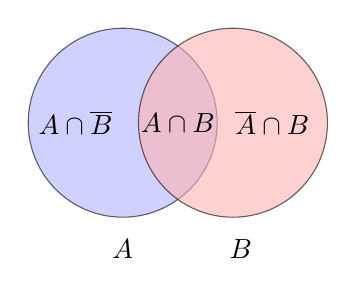
\begin{tikzpicture}
    % Draw set A
    \begin{scope}
        \draw[fill=blue!30, opacity=0.6] (2,2) circle (1.2);
    \end{scope}

    % Draw set B
    \begin{scope}
        \draw[fill=red!30, opacity=0.6] (3.4,2) circle (1.2);
    \end{scope}

    % Labels
    \node at (2,0.4) {$A$};
    \node at (3.5,0.4) {$B$};
    \node at (1.4,2) {$A \cap \overline{B}$};
    \node at (3.9,2) {$\overline{A} \cap B$};
    \node at (2.7,2) {$A \cap B$};
\end{tikzpicture}
\end{center}


The event $A$ consists of two mutually exclusive events $A \cap \overline{B}$ and $A \cap B$. Therefore
$$P(A) = P(A \cap \overline{B})+P(A \cap B)$$
Similarly,
$$P(B) = P(\overline{A} \cap B)+P(A \cap B)$$
Now,
\begin{align*}
    P(A \cup B) &= P(A \cap \overline{B})+P(A \cap B)+P(\overline{A} \cap B) \\
    &= \left[P(A) - P(A \cap B)\right] + P(A \cap B) + \left[P(B) - P(A \cap B)\right] \\
    &=P(A) + P(B) - P(A \cap B)
\end{align*}
\hfill\(\blacksquare\)

\textbf{Example}: Consider a fair six-sided die, and define two events:
\begin{itemize}
    \item $A$: The event that the die shows an odd number (i.e., $A = \{1, 3, 5\}$)
    \item $B$: The event that the die shows a number greater than or equal to 4 (i.e.,  $A = \{4,5,6\}$)
\end{itemize}


The union of \( A \) and \( B \) is the event that either event \( A \) or event \( B \) occurs (or both). The union of \( A \) and \( B \) is denoted by:

\[
A \cup B = \{1, 3, 5, 4, 6\} = \{1, 3, 4, 5, 6\}
\]

To find the probability of the union \( P(A \cup B) \), we use the formula:

\[
P(A \cup B) = P(A) + P(B) - P(A \cap B)
\]

\begin{itemize}
    \item \( P(A) = \frac{3}{6} = 0.5 \) (since there are 3 odd numbers: 1, 3, 5)
    \item \( P(B) = \frac{3}{6} = 0.5 \) (since there are 3 numbers \( \geq 4 \): 4, 5, 6)
    \item \( P(A \cap B) = \frac{1}{6} = \frac{1}{3} \) (since 5 is the only number that is both odd and \( \geq 4 \))
\end{itemize}

So, the probability of \( A \cup B \) is:

\[
P(A \cup B) = 0.5 + 0.5 - \frac{1}{3} = 1 - \frac{1}{3} = \frac{2}{3}
\]

Thus, the probability of rolling a die and getting either an odd number or a number greater than or equal to 4 is \( \frac{2}{3} \).


\begin{textbox}
\textbf{Theorem}: For any three events $A$, $B$ and $C$ (not necessarily mutually exclusive),
\begin{align*}
    P(A \cup B \cup C) = &P(A) + P(B) +P(C) - P(A \cap B) - P(B \cap C) \\
    &- P(A \cap C)  + P(A \cap B \cap C)
\end{align*}
\end{textbox}

\textbf{Proof}: We begin by applying the two-event formula to $A \cup (B \cup C)$:

$$P(A \cup B \cup C) = P(A) + P(B \cup C) - P(A \cap (B \cup C))$$

Now, apply the two-event formula to $P(B \cup C)$:

$$P(B \cup C) = P(B) + P(C) - P(B \cap C)$$

Also, apply distributivity to expand \( P(A \cap (B \cup C)) \):

\begin{align*}
P(A \cap (B \cup C)) &= P((A \cap B) \cup (A \cap C)) \\
&= P(A \cap B) + P(A \cap C) - P(A \cap B \cap C)
\end{align*}

Substituting back into the original expression:

\begin{align*}
P(A \cup B \cup C) &= P(A) + \big[ P(B) + P(C) - P(B \cap C) \big] \\
&\quad - \big[ P(A \cap B) + P(A \cap C) - P(A \cap B \cap C) \big] \\
&= P(A) + P(B) + P(C) - P(B \cap C) \\
&\quad - P(A \cap B) - P(A \cap C) + P(A \cap B \cap C)
\end{align*}
\hfill\(\blacksquare\)

\begin{textbox}
\textbf{Theorem}: Let \( A_1, A_2, \ldots, A_n \) be $n$ number of events of a random experiment. Then the probability of their union is given by:

\begin{align*}
P\left( \bigcup_{i=1}^n A_i \right)
= &\sum_{i=1}^{n} P(A_i)
- \sum_{1 \le i < j \le n} P(A_i \cap A_j) \\
&+ \sum_{1 \le i < j < k \le n} P(A_i \cap A_j \cap A_k)
- \cdots \\
&+ (-1)^{n+1} P(A_1 \cap A_2 \cap \cdots \cap A_n)
\end{align*}

\end{textbox}
The proof of this theorem is left as an exercise.

\begin{textbox}
    \textbf{Theorem}: If $A$ and $B$ are two events of a random experiment, then the probability that exactly one of them occurs is given by
    $$P(\text{exactly one of } A \text{ or } B) = P(A) + P(B) - 2P(A \cap B)$$
\end{textbox}
\textbf{Proof}: The event ``exactly one of $A$ or $B$ occurs'' means either $A$ happens and $B$ doesn't, or $B$  happens and $A$ doesn't. That means the event:
\[
(A \cap \overline{B}) \cup (\overline{A} \cap B)
\]

% Since the events $(A \cap \overline{B})$ and $(\overline{A} \cap B)$ are disjoint, so:
% \[
% P((A \cap \overline{B}) \cup (\overline{A} \cap B)) = P(A \cap \overline{B}) + P(\overline{A} \cap B)
% \]

% Now,
% \[
% P(A \cap \overline{B}) = P(A) - P(A \cap B)
% \]
% \[
% P(\overline{A} \cap B) = P(B) - P(A \cap B)
% \]

% Therefore,
% \[
% P(\text{exactly one of } A \text{ or } B) = P(A) + P(B) - 2P(A \cap B)
% \]

\begin{center}
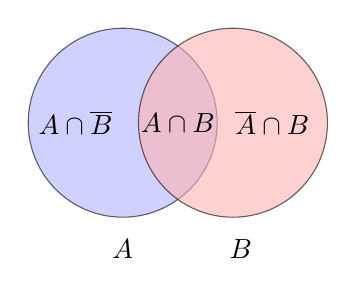
\begin{tikzpicture}
    % Draw set A
    \begin{scope}
        \draw[fill=blue!30, opacity=0.6] (2,2) circle (1.2);
    \end{scope}

    % Draw set B
    \begin{scope}
        \draw[fill=red!30, opacity=0.6] (3.4,2) circle (1.2);
    \end{scope}

    % Labels
    \node at (2,0.4) {$A$};
    \node at (3.5,0.4) {$B$};
    \node at (1.4,2) {$A \cap \overline{B}$};
    \node at (3.9,2) {$\overline{A} \cap B$};
    \node at (2.7,2) {$A \cap B$};
\end{tikzpicture}
\end{center}

We can see it from the Venn diagram:
\begin{align*}
    P((A \cap \overline{B}) \cup (\overline{A} \cap B)) &= P(A \cup B) - P(A \cap B) \\
    &= (P(A) + P(B) - P(A \cap B)) - P(A \cap B) \\
    &= P(A) + P(B) - 2P(A \cap B)
\end{align*}

Therefore,
\[
P(\text{exactly one of } A \text{ or } B) = P(A) + P(B) - 2P(A \cap B)
\]
\hfill\(\blacksquare\)

\begin{textbox}
\textbf{Boole's Inequality}: Let \( A_1, A_2, \ldots, A_n \) be $n$ events of a random experiment. Then:

\[
P\left( \bigcup_{i=1}^{n} A_i \right) \leq \sum_{i=1}^{n} P(A_i)
\]
\end{textbox}

\textbf{Proof}: We prove the inequality by induction on \( n \).

\underline{Base Case:} For \( n = 1 \),
\[
P(A_1) = P(A_1)
\]
so the inequality holds with equality.

\underline{Inductive Step:} Assume the inequality holds for \( n = k \), i.e.,
\[
P\left( \bigcup_{i=1}^{k} A_i \right) \leq \sum_{i=1}^{k} P(A_i)
\]

Now consider \( n = k+1 \). Let \( B = \bigcup_{i=1}^{k} A_i \). Then:
\[
P\left( \bigcup_{i=1}^{k+1} A_i \right) = P(B \cup A_{k+1})
\]

Using the formula for the union of two events:
\[
P(B \cup A_{k+1}) = P(B) + P(A_{k+1}) - P(B \cap A_{k+1}) \leq P(B) + P(A_{k+1})
\]

Applying the induction hypothesis to \( P(B) \):
\[
P(B \cup A_{k+1}) \leq \sum_{i=1}^{k} P(A_i) + P(A_{k+1}) = \sum_{i=1}^{k+1} P(A_i)
\]

Thus, the inequality holds for \( n = k+1 \). By the principle of mathematical induction, the inequality holds for all \( n \in \mathbb{N} \).
\hfill\(\blacksquare\)


Boole's inequality provides a simple and conservative upper bound for the probability of the union of multiple events. This is important because, without detailed knowledge of the relationships between the events (e.g., how much they overlap), we can still estimate the probability that at least one of the events occurs by adding their individual probabilities.

\textbf{Example}: If you have three events with probabilities:
\[
P(A_1) = 0.3, \quad P(A_2) = 0.5, \quad P(A_3) = 0.7,
\]
but you don’t know the intersections between them, Boole’s inequality will tell you that the probability of at least one occurring is at most:

\[
P(A_1 \cup A_2 \cup A_3) \leq 0.3 + 0.5 + 0.7 = 1.5
\]

Since probabilities cannot exceed 1, this shows that the bound is very loose, but it is still useful for getting a rough estimate.


\begin{textbox}
\textbf{Bonferroni's inequality}: Let \( A_1, A_2, \ldots, A_n \) be events of a random experiment. Then:

\[
P\left( \bigcap_{i=1}^n A_i \right) \geq \sum_{i=1}^n P(A_i) - (n - 1)
\]
\end{textbox}

\textbf{Proof:} We proceed by induction on \( n \).

\underline{Base case:} For \( n = 2 \),
we begin with the identity:
\[
P(A_1 \cup A_2) = P(A_1) + P(A_2) - P(A_1 \cap A_2)
\]

Using the axiom that \( P(A_1 \cup A_2) \leq 1 \), we substitute:
\[
P(A_1) + P(A_2) - P(A_1 \cap A_2) \leq 1
\]

Rearranging:
\[
 P(A_1 \cap A_2) \geq P(A_1) + P(A_2) - 1
\]

So the inequality holds for $n = 2$.

\underline{Inductive step:} Assume the result holds for \( n = k \), i.e.,
\[
P\left( \bigcap_{i=1}^{k} A_i \right) \geq \sum_{i=1}^{k} P(A_i) - (k - 1)
\]

Let \( B = \bigcap_{i=1}^{k} A_i \). Then:
\[
P\left( \bigcap_{i=1}^{k+1} A_i \right) = P(B \cap A_{k+1}) \geq P(B) + P(A_{k+1}) - 1
\]

Using the induction hypothesis:
\[
P(B \cap A_{k+1}) \geq \left( \sum_{i=1}^{k} P(A_i) - (k - 1) \right) + P(A_{k+1}) - 1 = \sum_{i=1}^{k+1} P(A_i) - k
\]

Therefore, the inequality holds for \( n = k + 1 \). By induction, it holds for all \( n \in \mathbb{N} \). \

The Bonferroni inequality for intersections provides a lower bound for the probability of the intersection of multiple events.
\hfill\(\blacksquare\)

\textbf{Example}: Consider three events \( A_1 \), \( A_2 \), and \( A_3 \) with probabilities:

\[
P(A_1) = 0.6, \quad P(A_2) = 0.5, \quad P(A_3) = 0.7
\]

Using Bonferroni’s inequality, the lower bound for the probability that all three events occur is:

\[
P(A_1 \cap A_2 \cap A_3) \geq 0.6 + 0.5 + 0.7 - 2 = 0.8
\]

Thus, the probability that all three events occur simultaneously is at least \( 0.8 \).


\section{Conditional Probability}

Conditional probability is the probability of an event occurring given that another event has already occurred.

\begin{textbox}
    Let $A$ and $B$ be two events of a random experiment. The \textbf{conditional probability} of event \( A \) given that event \( B \) has already occurred is defined as:

\[
P(A \mid B) = \frac{P(A \cap B)}{P(B)}, \quad \text{provided} \, P(B) \neq 0
\]
\end{textbox}

This formula tells us how likely event \( A \) is, given that we know event \( B \) has happened. The idea is that we restrict our sample space to the outcomes where \( B \) occurs, and then we compute the probability of \( A \) within this restricted sample space.

\textbf{Example}: Let's define two events when rolling a fair six-sided die:

\begin{itemize}
    \item \( A \): The event that the die shows an \textit{even face}, i.e., \( A = \{2, 4, 6\} \).
    \item \( B \): The event that the die shows a \textit{multiple of 3}, i.e., \( B = \{3, 6\} \).
\end{itemize}
\begin{align*}
    P(A) &= P(\{2, 4, 6\})= \frac{3}{6} = \frac{1}{2} \\
    P(B) &= P(\{3, 6\})=  \frac{2}{6} = \frac{1}{3} \\
    P(A \cap B) &= P(\{6\}) = \frac{1}{6}
\end{align*}

The conditional probability of \( A \) given \( B \) is:

\[
P(A \mid B) = \frac{P(A \cap B)}{P(B)} = \dfrac{\frac{1}{6}}{\frac{1}{3}}  = \frac{1}{2}
\]

The conditional probability of \( B \) given \( A \) is:

\[
P(B \mid A) = \frac{P(A \cap B)}{P(A)} =\frac{\frac{1}{6}}{\frac{1}{2}} = \frac{1}{3}
\]

\begin{textbox}
\textbf{Multiplication Rule of Probabilities}: If \( A \) and \( B \) are any events in the sample space \( S \), then:
\begin{align*}
    P(A \cap B) &= P(A) \cdot P(B \mid A), \quad \text{if } P(A) \neq 0 \\
 &= P(B) \cdot P(A \mid B), \quad \text{if } P(B) \neq 0
\end{align*}
\end{textbox}
The second rule follows directly from the definition of conditional probability by multiplying both sides by \( P(B) \).
The first rule is obtained from the second by simply switching the roles of \( A \) and \( B \).

\section{Rule of Total Probability}

The Rule of Total Probability allows us to compute the probability of an event based on a partition of the sample space.

\subsection{For Two Events}
\begin{textbox}
    If \( B \) and its complement \( \overline{B} \) form a partition of the sample space (i.e., mutually exclusive and collectively exhaustive events), then for any event \( A \):

\[
P(A) = P(A \mid B)P(B) + P(A \mid \overline{B})P(\overline{B})
\]
\end{textbox}
\textbf{Proof}: Let \( B \) and \( \overline{B} \) form a partition (i.e., mutually exclusive and exhaustive events) of the sample space. Then any event \( A \) can be expressed as:

\[
A = (A \cap B) \cup (A \cap \overline{B})
\]

Since the sets \( A \cap B \) and \( A \cap \overline{B} \) are disjoint, the two parts are mutually exclusive. So:

\[
P(A) = P(A \cap B) + P(A \cap \overline{B})
\]

Using the definition of conditional probability:

\[
P(A \cap B) = P(A \mid B)P(B), \quad P(A \cap \overline{B}) = P(A \mid \overline{B})P(\overline{B})
\]

Substituting:

\[
P(A) = P(A \mid B)P(B) + P(A \mid \overline{B})P(\overline{B})
\]
\hfill\(\blacksquare\)

\subsection{For Multiple Events}

\begin{textbox}

Let \( B_1, B_2, \dots, B_n \) be a partition of the sample space (i.e., mutually exclusive and collectively exhaustive events). Then for any event \( A \):

\[
P(A) = \sum_{i=1}^{n} P(A \mid B_i)P(B_i)
\]
\end{textbox}

\textbf{Proof}: Let \( B_1, B_2, \dots, B_n \) be a partition of the sample space, i.e.,

\begin{itemize}
    \item The events \( B_i \) are mutually exclusive: \( B_i \cap B_j = \emptyset \) for \( i \ne j \)
    \item The events \( B_i \) are collectively exhaustive: \( \bigcup_{i=1}^n B_i = S \)
\end{itemize}

Then for any event \( A \subseteq S \):

\[
A = A \cap S = A \cap \left( \bigcup_{i=1}^n B_i \right) = \bigcup_{i=1}^n (A \cap B_i)
\]

Since the \( B_i \) are disjoint, so are the \( A \cap B_i \), so:

\[
P(A) = \sum_{i=1}^n P(A \cap B_i)
\]

Using conditional probability:

\[
P(A \cap B_i) = P(A \mid B_i)P(B_i)
\]

Therefore:

\[
P(A) = \sum_{i=1}^n P(A \mid B_i)P(B_i)
\]
\hfill\(\blacksquare\)

\textbf{Example}: Suppose a factory has three machines:

\begin{itemize}
    \item Machine \( M_1 \) produces 30\% of the items, with a defect rate of 1\%.
    \item Machine \( M_2 \) produces 50\% of the items, with a defect rate of 2\%.
    \item Machine \( M_3 \) produces 20\% of the items, with a defect rate of 3\%.
\end{itemize}

Let \( D \) be the event that an item is defective. We are asked to find \( P(D) \), the total probability that a randomly selected item is defective.

Using the Rule of Total Probability:

\[
P(D) = P(D \mid M_1)P(M_1) + P(D \mid M_2)P(M_2) + P(D \mid M_3)P(M_3)
\]

Substituting the known values:

\begin{align*}
    P(D) &= (0.01 \times 0.30) + (0.02 \times 0.50) + (0.03 \times 0.20) \\
    &= 0.003 + 0.010 + 0.006 = 0.019
\end{align*}

The probability that a randomly chosen item is defective is $0.019$ or $1.9$\%.


\section{Bayes' Theorem}
Bayes' Theorem is a fundamental result in probability theory that arises directly from the definition of conditional probability and the Rule of Total Probability.
\begin{textbox}
    \textbf{Bayes' Theorem}: Let \( B_1, B_2, \ldots, B_n \) be a partition of the sample space (i.e., mutually exclusive and collectively exhaustive events) and none of which has zero probability i.e. \( P(B_i) > 0 \) for all \( i \), then for any event \( A \) with \( P(A) > 0 \), the probability of \( B_r \) given \( A \) is:
\[
P(B_r \mid A) = \frac{P(B_r) \cdot P(A \mid B_r)}{\sum_{i=1}^{n} P(B_i) \cdot P(A \mid B_i)}
\]

for \( r = 1, 2, \ldots, n \).
\end{textbox}
\textbf{Proof}: Let \( B_1, B_2, \ldots, B_n \) be a partition of the sample space \( S \) such that:
\begin{itemize}
    \item The events \( B_i \) are mutually exclusive: \( B_i \cap B_j = \emptyset \) for \( i \neq j \),
    \item The union of the \( B_i \)'s covers the whole sample space: \( \bigcup_{i=1}^n B_i = S \),
    \item \( P(B_i) > 0 \) for all \( i \).
\end{itemize}

Let \( A \) be any event with \( P(A) > 0 \). By the definition of conditional probability:

\[
P(B_r \mid A) = \frac{P(B_r \cap A)}{P(A)}
\]

We apply the Multiplication Rule of Probabilities:

\[
P(B_r \cap A) = P(B_r) \cdot P(A \mid B_r)
\]

So:

\[
P(B_r \mid A) = \frac{P(B_r) \cdot P(A \mid B_r)}{P(A)}
\]

Now, using the Rule of Total Probability:

\[
P(A) = \sum_{i=1}^n P(B_i) \cdot P(A \mid B_i)
\]

Substitute this into the denominator:

\[
P(B_r \mid A) = \frac{P(B_r) \cdot P(A \mid B_r)}{\sum_{i=1}^{n} P(B_i) \cdot P(A \mid B_i)}
\]
\hfill\(\blacksquare\)

\textbf{Example}: Suppose in a dataset of 1000 emails, 200 are identified as spam and 800 as non-spam. Among the spam emails, 80 contain the word `discount', while 80 of the non-spam emails also contain this word. We need to calculate the probability that an email is spam given that it contains the word `discount'.
\begin{itemize}
    \item \( P(S) = \dfrac{200}{1000} = 0.2 \): Probability that an email is spam.
    \item \( P(\overline{S}) = \dfrac{800}{1000} = 0.8 \): Probability that an email is not spam.
    \item \( P(D \mid S) =\dfrac{80}{200} =  0.4 \): Probability that the word ``discount'' appears in a spam email.
    \item \( P(D \mid \overline{S})=\dfrac{80}{800} = 0.1 \): Probability that ``discount'' appears in a non-spam email.
\end{itemize}

We want to find the probability that an email is spam given that it contains the word ``discount'', i.e., \( P(S \mid D) \).

Using Bayes' Theorem:
\[
P(S \mid D) = \frac{P(S) \cdot P(D \mid S)}{P(S) \cdot P(D \mid S) + P(\overline{S}) \cdot P(D \mid \overline{S})}
\]

Substituting the values:
\[
P(S \mid D) = \frac{0.2 \times 0.4}{0.2 \cdot 0.4 + 0.8 \cdot 0.1}
= \frac{0.08}{0.08 + 0.08}
= \frac{0.08}{0.16} = 0.5
\]

So, the probability that the email is spam given it contains the word ``discount'' is \( 50\% \). Even though only \(20\%\) of all emails are spam, once we see the word ``discount'' the chance the email is spam rises to \(50\%\), because that word is much more common in spam than in legitimate messages.

\subsection{Importance of Bayes' Theorem and Updating Probability}

Bayes’ Theorem is important because it provides a mathematical framework for updating probabilities when new information becomes available. In real-world terms, it helps us refine our beliefs or predictions as we gather more data.

Suppose we want to determine the probability of an event \( A \), such as an email being spam. Initially, we rely on prior knowledge, which is represented by the prior probability \( P(A) \). Now, imagine we observe some new evidence \( B \), such as the presence of a specific word like ``discount'' in the email.

Bayes' Theorem helps us compute the updated probability \( P(A \mid B) \), known as the posterior probability, using the following formula:

\[
P(A \mid B) = \frac{P(A) \cdot P(B \mid A)}{P(B)}
\]

Here:
\begin{itemize}
    \item \( P(A) \) is the \textbf{prior probability} — our initial belief (prediction) about the event \( A \).
    \item \( P(B \mid A) \) is the \textbf{likelihood} — the probability of observing evidence \( B \) given that \( A \) is true.
    \item \( P(B) \) is the \textbf{marginal probability} of observing evidence \( B \) under all possible conditions.
    \item \( P(A \mid B) \) is the \textbf{posterior probability} — our updated belief (prediction)  about \( A \) after observing \( B \).
\end{itemize}

This formula enables us to revise our estimate of the probability of \( A \) whenever new information \( B \) becomes available. Depending on the relationship between \( A \) and \( B \), the posterior probability may be higher or lower than the prior, reflecting the impact of the new evidence.

\subsection{The Base Rate Fallacy and Bayes' Theorem}

\begin{textbox}
The \textbf{base rate fallacy} is a cognitive bias which occurs when people wrongly judge the probability of an event (like having a disease) by focusing on new information (such as a test result) while ignoring how rare or common the event is in the general population.
\end{textbox}

\medskip

Imagine you're told that a COVID-19 test is 95-99\% accurate. You take the test, and it comes back \textbf{positive}. Does that mean you're almost certainly infected with 95\% possibility?

Not necessarily. This is where the \textbf{base rate fallacy} comes into play—a common error in reasoning where people ignore the underlying probability of an event (known as the \textit{base rate}) and instead focus too heavily on new information, like a test result.

To illustrate this idea, suppose we are testing a population where only 1\% of individuals are actually infected with COVID-19. Consider the characteristics of the test:

\begin{itemize}
    \item \textbf{Prevalence (Base Rate)}: $P(\text{COVID}) = 0.01$
    \item \textbf{Sensitivity (True Positive Rate)}: $P(\text{Positive} \mid \text{COVID}) = 0.99$
    \item \textbf{Specificity (True Negative Rate)}: $P(\text{Negative} \mid \text{No COVID}) = 0.95$
\end{itemize}

Now the question is, if a person tests positive, what is the probability that they actually have COVID-19?


To answer this, we apply \textbf{Bayes’ Theorem}:

\[
P(\text{COVID} \mid \text{Positive}) = \frac{P(\text{Positive} \mid \text{COVID}) \cdot P(\text{COVID})}{P(\text{Positive})}
\]

We compute the total probability of a positive test as:

\[
P(\text{Positive}) = P(\text{Positive} \mid \text{COVID}) \cdot P(\text{COVID}) + P(\text{Positive} \mid \text{No COVID}) \cdot P(\text{No COVID})
\]
\[
= 0.99\times 0.01 + 0.05 \times 0.99 = 0.0099 + 0.0495 = 0.0594
\]

Now, substituting into Bayes' formula:

\[
P(\text{COVID} \mid \text{Positive}) = \frac{0.99 \times 0.01}{0.0594} \approx \frac{0.0099}{0.0594} \approx 0.167
\]

That is, even with a \textbf{positive test result}, the probability of actually having COVID is only around \textbf{16.7\%}. Most people wrongly assume that a positive result from a highly accurate test means they almost certainly have the disease. However, because COVID-19 is relatively rare in the population (a low base rate), even highly accurate tests produce many false positives. This is the essence of the \textbf{base rate fallacy}: ignoring the background prevalence (base rate) of the disease and overestimating the significance of the test result.

\textbf{Example}: Imagine testing 10{,}000 people:

\begin{itemize}
    \item 1\% are infected $\Rightarrow$ 100 people have COVID.
    \item 99\% are not infected $\Rightarrow$ 9{,}900 people do not have COVID.
\end{itemize}

Now apply the test:

\begin{itemize}
    \item Among 100 infected people 99 test positive (99\% true positives).
    \item Among 9{,}900 uninfected people 9{,}405 test negative (95\% true positives) meaning 495 test positive (5\% false positives).
\end{itemize}

\noindent
So, total positive tests = 99 (true) + 495 (false) = 594

Probability of actually having COVID given a positive test = $ \dfrac{99}{594} \approx 16.7\% $

\section{Statistical Independence of Events}

If $A$ and $B$ are any two events in a sample space $S$, we say that ``$A$ is independent of $B$'' if:

$$
P(A \mid B) = P(A)
$$

This means that knowing whether or not $B$ has occurred ``does not change'' the probability of $A$ occurring.

From the definition of conditional probability:

$$
P(A \mid B) = \frac{P(A \cap B)}{P(B)},
$$

if we substitute and rearrange the condition $P(A \mid B) = P(A)$, we get:

$$
\frac{P(A \cap B)}{P(B)} = P(A) \quad \Rightarrow \quad P(A \cap B) = P(A) \cdot P(B)
$$

Thus, another equivalent definition of independence is:

$$
P(A \cap B) = P(A) \cdot P(B)
$$

Now, to check whether $B$ is independent of $A$, we look at:

$$
P(B \mid A) = \frac{P(B \cap A)}{P(A)} = \frac{P(A \cap B)}{P(A)}
$$

Since we just showed that $P(A \cap B) = P(A) \cdot P(B)$, substitute:

$$
P(B \mid A) = \frac{P(A) \cdot P(B)}{P(A)} = P(B)
$$

Thus, $B$ is also independent of $A$.

\begin{textbox}
If \( A \) is independent of \( B \), then \( B \) is also independent of \( A \). Therefore, we say that \( A \) and \( B \) are \textbf{mutually independent}.
\end{textbox}

\begin{textbox}
\textbf{Multiplication Rule for Independent Events}: Two events $A$ and $B$ are (mutually) independent events if and only if
$$P( A \cap B ) = P( A ) \cdot P( B )$$
\end{textbox}

\textbf{Example}: Consider the experiment of rolling two fair six-sided dice, and consider the following events:
\begin{itemize}
    \item \( A \): The first die shows a 1.
    \[ A = \{(1,1), (1,2), (1,3), (1,4), (1,5), (1,6)\} \]
    \item \( B \): The second die shows a 2.
    \[ B = \{(1,2), (2,2), (3,2), (4,2), (5,2), (6,2)\} \]
\end{itemize}

The total number of outcomes in the sample space is \( 6 \times 6 = 36 \).

We compute:
\[
P(A) = \frac{6}{36} = \frac{1}{6}, \quad P(B) = \frac{6}{36} = \frac{1}{6}
\]
\[
A \cap B = \{(1,2)\} \quad \Rightarrow \quad P(A \cap B) = \frac{1}{36}
\]

Since
\[
P(A \cap B) = P(A) \cdot P(B) = \frac{1}{6} \cdot \frac{1}{6} = \frac{1}{36},
\]
we conclude that the events \( A \) and \( B \) are \textbf{independent}.

\begin{textbox}
\textbf{Theorem:}
If the events \( A \) and \( B \) are independent, then the following pairs of events are also independent:
\[
\text{(1) } A \text{ and } \overline{B}, \quad \text{(2) } \overline{A} \text{ and } B, \quad \text{(3) } \overline{A} \text{ and } \overline{B}
\]
\end{textbox}
\textbf{Proof:}

\begin{itemize}
  \item[1.] Since \( A \) and \( B \) are independent, we have:
  \[
  P(A \cap B) = P(A)\cdot P(B)
  \]
  Then,
  \[
  P(A \cap \overline{B}) = P(A) - P(A \cap B) = P(A) - P(A)\cdot P(B) = P(A)(1 - P(B)) = P(A)\cdot P(\overline{B})
  \]
  So, \( A \) and \( \overline{B} \) are independent.

  \item[2.] Similarly,
  \[
  P(\overline{A} \cap B)  = P(B) - P(A \cap B) = P(B) - P(A)\cdot P(B) = P(B)(1 - P(A)) = P(\overline{A})\cdot P(B)
  \]
  So, \( \overline{A} \) and \( B \) are independent.

  \item[3.] Finally,
  \[
  P(\overline{A} \cap \overline{B}) = P(\overline{A \cup B}) = 1 - P(A \cup B) = 1 - [P(A) + P(B) - P(A \cap B)]
  \]
  \[
  = 1 - [P(A) + P(B) - P(A)\cdot P(B)] = (1 - P(A))(1 - P(B)) = P(\overline{A})\cdot P(\overline{B})
  \]
  So, \( \overline{A} \) and \( \overline{B} \) are also independent.
\end{itemize}
\hfill\(\blacksquare\)

\begin{textbox}
    \textbf{Theorem}: If A and B are independent events, then:

\[
P(A \cup B) = 1 - P(\overline{A})\cdot P(\overline{B})
\]
\end{textbox}

\textbf{Proof}: Using the formula for the union of two events:

\[
P(A \cup B) = P(A) + P(B) - P(A \cap B)
\]

Since \( A \) and \( B \) are independent, \( P(A \cap B) = P(A)\cdot P(B) \), so:

\begin{align*}
    P(A \cup B) &= P(A) + P(B) - P(A)\cdot P(B) \\
    &= 1 - \left(1 - P(A) - P(B) + P(A)\cdot P(B)\right) \\
    &= 1- (1-P(A))(1-P(B)) \\
    &= 1 - P(\overline{A})P(\overline{B})
\end{align*}
\hfill\(\blacksquare\)

\subsection{Pairwise vs. Mutual Independence of Multiple Events}

Let \( A \), \( B \), and \( C \) be three events in a sample space \( S \). The events \( A \), \( B \), and \( C \) are said to be \textbf{pairwise independent} if:
\[
\begin{aligned}
P(A \cap B) &= P(A) \cdot P(B), \\
P(A \cap C) &= P(A) \cdot P(C), \\
P(B \cap C) &= P(B) \cdot P(C)
\end{aligned}
\]

The events \( A \), \( B \), and \( C \) are said to be \textbf{mutually independent} if:
\begin{itemize}
    \item They are pairwise independent, and
    \item The joint probability satisfies:
    \[
    P(A \cap B \cap C) = P(A) \cdot P(B) \cdot P(C)
    \]
\end{itemize}

\textbf{Note:} Mutual independence \emph{implies} pairwise independence, but the converse is not necessarily true.

\subsection{Mutually Exclusive and Independent Events}

Let \( A \) and \( B \) be two events in a sample space.

\begin{itemize}
    \item If \( A \) and \( B \) are \textbf{mutually exclusive}, then:
    \[
    A \cap B = \emptyset \quad \Rightarrow \quad P(A \cap B) = 0
    \]

    \item If \( A \) and \( B \) are \textbf{independent}, then:
    \[
    P(A \cap B) = P(A) \cdot P(B)
    \]
\end{itemize}

If both conditions are true, then:
\[
P(A) \cdot P(B) = 0
\]
This implies that either \( P(A) = 0 \), \( P(B) = 0 \), or both.

\begin{textbox}
Two events \( A \) and \( B \) cannot be both mutually exclusive and independent unless at least one of them has probability zero.
\end{textbox}


In terms of a Venn diagram, the independence of events implies that the overlap between sets \( A \) and \( B \) (i.e., \( A \cap B \)) should be such that its area (probability) equals the product of the areas (probabilities) of each individual circle.

\begin{center}
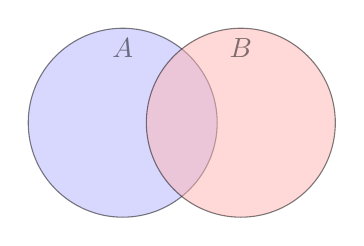
\begin{tikzpicture}
  % Draw event A
  \draw[fill=blue!30, opacity=0.5] (2,2) circle (1.2) node[left=20pt, above=20pt] {\(A\)};

  % Draw event B
  \draw[fill=red!30, opacity=0.5] (3.5,2) circle (1.2) node[right=20pt, above=20pt] {\(B\)};
\end{tikzpicture}
\end{center}

This is different from mutually exclusive events, where the sets do not overlap at all. Both the condition will be satisfied if the area of at least one of the circle is zero.

\subsection{Reliability Analysis using Statistical Independence}

Reliability analysis is the branch of engineering concerned with estimating the failure
rates of systems. If a machine has a reliability of $0.95$ over $1$ year, it means there is a $95\%$ chance that it will work without failure for the entire year. In many systems, components are arranged either in \textit{series} or in \textit{parallel}, and the system's reliability depends on the configuration.

\begin{enumerate}

\item \textbf{System with Components in Series}:

Consider a system with two components, \( A \) and \( B \), connected in \textbf{series}. In this setup, the system will work only if \textbf{both} components function properly.

\begin{center}
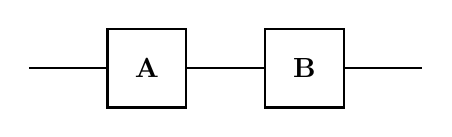
\begin{tikzpicture}[thick]
  % Draw lines before and after the blocks
  \draw (0,0) -- (1,0);
  \draw (2,0) -- (3,0);
  \draw (4,0) -- (5,0);

  % Draw component A
  \draw (1, -0.5) rectangle (2, 0.5);
  \node at (1.5, 0) {\textbf{A}};

  % Draw component B
  \draw (3, -0.5) rectangle (4, 0.5);
  \node at (3.5, 0) {\textbf{B}};
\end{tikzpicture}
\end{center}

Suppose the probability that $A$ functions is given by $P(A) = 0.96$, and the probability that $B$ functions is given by
$P(B) = 0.92$. Assuming that the components function independently, the probability that the system works is:

\[
\begin{aligned}
P(\text{System functions}) &= P(A \cap B) \\
&= P(A) \cdot P(B) \\
&= 0.96\times 0.92 = 0.8832
\end{aligned}
\]

Since both components must function, the system's reliability is lower than that of either component individually. The more components in series, the more chances for failure.

\item \textbf{System with Components in Parallel}:

Now consider a system with two components, \( C \) and \( D \), connected in \textbf{parallel}. In this case, the system will function as long as \textbf{at least one} component functions.

\begin{center}
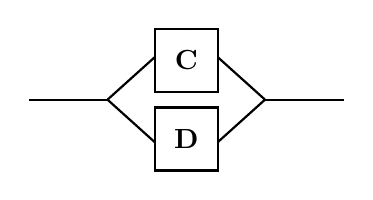
\begin{tikzpicture}[thick]
  % Input and output lines
  \draw (-2,0) -- (-1,0);
  \draw (1,0) -- (2,0);

  % Top branch with C
  \draw (-1,0) -- (0,0.9);
  \draw (0,0.9) -- (1,0);
  \draw (0,0.5) node[draw, fill=white, minimum size=8mm] {\textbf{C}};

  % Bottom branch with D
  \draw (-1,0) -- (0,-0.9);
  \draw (0,-0.9) -- (1,0);
  \draw (0,-0.5) node[draw, fill=white, minimum size=8mm] {\textbf{D}};
\end{tikzpicture}
\end{center}

Suppose the probabilities that the components function are:
\[
P(C) = 0.88, \quad P(D) = 0.85
\]

Assuming independence, the probability that the system functions is given by:

\[
\begin{aligned}
P(\text{System functions}) &= P(C \cup D) \\
&= P(C) + P(D) - P(C \cap D) \\
&= P(C) + P(D) - P(C).P(D) \\
&= 0.88 + 0.85 - (0.88 \times 0.85) \\
&= 1.73 - 0.748 = 0.982
\end{aligned}
\]

In parallel systems, the system is more reliable than the individual components. This configuration adds redundancy, improving fault tolerance.
\end{enumerate}

\chapter{Random Variables and Probability Distributions}
\section{What is a Random Variable?}
In most cases, we can associate a real number with each elementary event in a sample space. For example, in a coin toss, we may assign the number \(1\) to the outcome `Head' and \(0\) to the outcome `Tail'. Similarly, when a die is thrown, the outcomes correspond to the numbers \(1, 2, 3, \dots, 6\), depending on which face appears on top.

This assignment of numerical values to outcomes allows us to define a function on the sample space. A real-valued function defined on the sample space is called a \textbf{random variable} (also referred to as a \textbf{stochastic variable}).

\begin{textbox}
    Let \( S \) be a sample space of a random experiment. A \textbf{random variable} is a function
\[
X : S \rightarrow \mathbb{R}
\]
where each outcome \( s \in S \) is mapped to a real number \( X(s) \).

\end{textbox}
\textbf{Note}: A random variable is denoted by an uppercase letter such as $X$ and $Y$. After experiment is conducted, the measured value of the random variable is denoted by a lowercase letter such as $x$
and $y$.

\subsection{Random Variable Types}

There are two main types:

\begin{enumerate}
    \item \textbf{Discrete Random Variable:} \\
    A discrete random variable takes on a countable\footnote{This means the values can be finite (like a die roll) or countably infinite (like the number of coin tosses until the first head).} number of distinct values. Let \( X \) be the number of heads obtained when a fair coin is tossed three times.
    The possible values of \( X \) are \( 0, 1, 2, 3 \). Since these values are countable and finite, \( X \) is a discrete random variable.

    \item \textbf{Continuous Random Variable:} \\
    A continuous random variable takes any value within a certain range of real numbers. The possible values are uncountable and include fractions and decimals. Let \( Y \) be the amount of time (in minutes) a customer waits in a queue at a bank.
    The variable \( Y \) can take any real value within a range, such as \( 0 \leq Y \leq 30 \), including fractions like \( 3.5 \) or \( 12.75 \). Hence, \( Y \) is a continuous random variable.
\end{enumerate}

\section{Probability Distribution}

To each value of a random variable \( X \), there corresponds a definite probability.
Let \( x_1, x_2, \dots, x_n \) be the possible values of \( X \), and let \( p_1, p_2, \dots, p_n \) be the corresponding probabilities such that:
\[
P(X = x_i) = p_i \quad \text{for } i = 1, 2, \dots, n
\]

A statement of these values along with their associated probabilities defines the {probability distribution} of the random variable \( X \).

\subsection{Probability Mass Function (PMF)}

The {Probability Mass Function (PMF)} is used for \textbf{discrete random variables}. It gives the probability that a discrete random variable \( X \) takes a specific value \( x_k \). The PMF is defined as:
\begin{textbox}
\[
p_X(x_k) = P(X = x_k)
\]
\end{textbox}
where \( x_k \) is a specific value of the random variable \( X \). The PMF satisfies the following properties:

\begin{enumerate}
    \item \( 0 \leq p_X(x_k) \leq 1 \) for all \( k \)
    \item \( \sum_{k} p_X(x_k) = 1 \)
\end{enumerate}

\textbf{Example}: Consider a discrete random variable \( X \) with the following distribution:
\[
p_X(x) = P(X = x) =
\begin{cases}
\frac{1}{4}, & \text{if } x = 1 \\
\frac{1}{2}, & \text{if } x = 2 \\
\frac{1}{4}, & \text{if } x = 3 \\
0, & \text{otherwise}
\end{cases}
\]

The PMF is visualized as follows:

\begin{center}
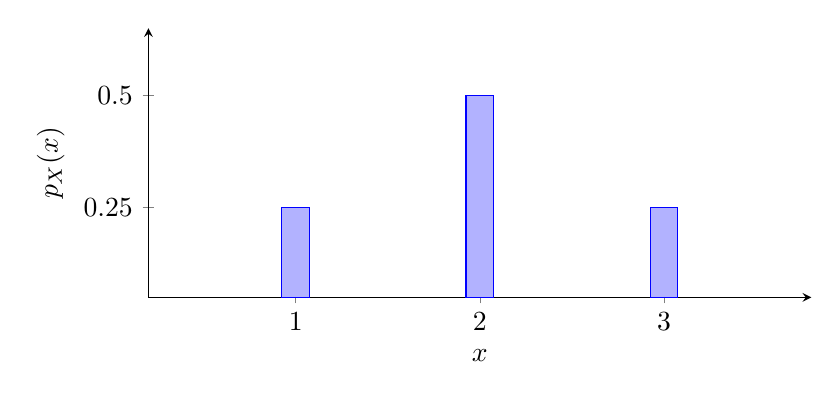
\begin{tikzpicture}
\begin{axis}[
    width=10cm,
    height=5cm,
    ybar,
    bar width=10pt,
    % axis x line=middle,
    % axis y line=middle,
    axis lines=left,
    xlabel={$x$},
    ylabel={$p_X(x)$},
    xtick={1,2,3},
    ytick={0,0.25,0.5},
    ymin=0.1, ymax=0.6,
    xmin=0.5, xmax=3.5,
    % ymajorgrids=true,
    enlargelimits=0.1,
    domain=1:3,
    samples=3,
    % every axis plot/.append style={
    %     ycomb,
    %     mark=*,
    %     line width=1pt,
    %     blue
    % }
]
\addplot+[] coordinates {(1,0.25) (2,0.5) (3,0.25)};
\end{axis}
\end{tikzpicture}
\end{center}

\subsection{Probability Density Function (PDF)}

The {Probability Density Function (PDF)} is used for \textbf{continuous random variables}. It is defined as a function $f_X$ such that the probability that a continuous random variable \( X \) lies within an interval \( [a, b] \) is given by the integral of $f_X$ over that interval:
\begin{textbox}
\[
P(a \leq X \leq b) = \int_a^b f_X(x) \, dx
\]
\end{textbox}
where \( f_X(x) \) is the PDF of \( X \). The PDF satisfies the following properties:

\begin{enumerate}
    \item \( f_X(x) \geq 0 \) for all \( x \)
    \item \( \int_{-\infty}^{\infty} f_X(x) \, dx = 1 \)
\end{enumerate}

\textbf{Example}: Consider a continuous random variable with the following distribution:
\[
f_X(x) =
\begin{cases}
1, & 0 \leq x \leq 1 \\
0, & \text{otherwise}
\end{cases}
\]
The PDF can be visualised as follows:


\begin{center}
\begin{tikzpicture}
\begin{axis}[
    width=10cm,
    height=5cm,
    axis lines=left,
    xlabel={$x$},
    ylabel={$f_X(x)$},
    xtick={0, 1},
    ytick={0, 0.5, 1},
    xmin=-0.2, xmax=1.2,
    ymin=0, ymax=1.2,
    % grid=major,
    % ymajorgrids=true,
    enlargelimits=0.05
]

\addplot[
    blue,
    very thick
] coordinates {
    (-1,0)
    (0,0)
};
\addplot[
    blue,
    dotted
] coordinates {
    (0,0)
    (0,1)
};
\addplot[
    blue,
    very thick
] coordinates {
    (0,1)
    (1,1)
};
\addplot[
    blue,
    dotted
] coordinates {
    (1,1)
    (1,0)
};
\addplot[
    blue,
    very thick
] coordinates {
    (1,0)
    (2,0)
};
\end{axis}
\end{tikzpicture}
\end{center}

\subsection{Cumulative Distribution}

The cumulative distribution gives the probability that a random variable takes a value less than or equal to a specified value. Mathematically \textbf{Cumulative Distribution Function} (CDF) of a random variable \( X \) is defined as:
\begin{textbox}
    \[
F_X(x) = P(X \leq x)
\]
\end{textbox}
This function gives the probability that \( X \) takes a value less than or equal to \( x \).

\textbf{CDF for Discrete Random Variables}

For a discrete random variable \( X \), the CDF is given by the sum of the probabilities for all values less than or equal to \( x \). If \( X \) takes the values \( x_1, x_2, \dots, x_n \), the CDF is:
\begin{textbox}
\[
F_X(x) = \sum_{x_k \leq x} P(X = x_k)
\]
\end{textbox}
This sum includes all the probabilities up to and including \( x \).

\textbf{Example:} Consider the random variable \( X \) representing the outcome of a fair six-sided die roll. The CDF for \( X \) is:
\[
F_X(x) =
\begin{cases}
0, & \text{if } x < 1 \\
\frac{1}{6}, & \text{if } 1 \leq x < 2 \\
\frac{2}{6}, & \text{if } 2 \leq x < 3 \\
\frac{3}{6}, & \text{if } 3 \leq x < 4 \\
\frac{4}{6}, & \text{if } 4 \leq x < 5 \\
\frac{5}{6}, & \text{if } 5 \leq x < 6 \\
1, & \text{if } x \geq 6
\end{cases}
\]

\begin{center}
\begin{tikzpicture}
\begin{axis}[
    width=10cm,
    height=5cm,
    axis lines=left,
    xlabel={$x$},
    ylabel={$F_X(x)$},
    xtick={0,1,2,3,4,5,6,7},
    ytick={0,1/6,2/6,3/6,4/6,5/6,1},
    xmin=0, xmax=7,
    ymin=0, ymax=1.1,
    % grid=major,
]

\addplot[
    blue,
    very thick
] coordinates {
    (0,0)
    (1,0)
};
\addplot[
    blue,
    dotted
] coordinates {
    (1,0)
    (1,1/6)
};
\addplot[
    blue,
    very thick
] coordinates {
    (1,1/6)
    (2,1/6)
};
\addplot[
    blue,
    dotted
] coordinates {
    (2,1/6)
    (2,2/6)
};
\addplot[
    blue,
    very thick
] coordinates {
    (2,2/6)
    (3,2/6)
};
\addplot[
    blue,
    dotted
] coordinates {
    (3,2/6)
    (3,3/6)
};
\addplot[
    blue,
    very thick
] coordinates {
    (3,3/6)
    (4,3/6)
};
\addplot[
    blue,
    dotted
] coordinates {
    (4,3/6)
    (4,4/6)
};
\addplot[
    blue,
    very thick
] coordinates {
    (4,4/6)
    (5,4/6)
};
\addplot[
    blue,
    dotted
] coordinates {
    (5,4/6)
    (5,5/6)
};
\addplot[
    blue,
    very thick
] coordinates {
    (5,5/6)
    (6,5/6)
};
\addplot[
    blue,
    dotted
] coordinates {
    (6,5/6)
    (6,1)
};
\addplot[
    blue,
    very thick
] coordinates {
    (6,1)
    (7,1)
};
\end{axis}
\end{tikzpicture}
\end{center}


\textbf{CDF for Continuous Random Variables}

For a continuous random variable \( X \), the CDF is obtained by integrating the probability density function (PDF) up to \( x \):
\begin{textbox}
\[
F_X(x) = \int_{-\infty}^{x} f_X(t) \, dt
\]
\end{textbox}
This represents the area under the PDF curve from \( -\infty \) to \( x \), giving the cumulative probability up to \( x \).

\textbf{Example:} Consider a continuous random variable \( X \) with a probability density function (PDF) \( f_X(x) = 1 \) for \( 0 \leq x \leq 1 \) (uniform distribution). The CDF is given by:
\[
F_X(x) =
\begin{cases}
0, & \text{if } x < 0 \\
x, & \text{if } 0 \leq x \leq 1 \\
1, & \text{if } x > 1
\end{cases}
\]
This is obtained by integrating the PDF:
\[
F_X(x) = \int_0^x 1 \,\cdot dt = x \quad \text{for} \quad 0 \leq x \leq 1
\]

\begin{center}
\begin{tikzpicture}
\begin{axis}[
    width=10cm,
    height=5cm,
    axis lines=left,
    xlabel={$x$},
    ylabel={$F_X(x)$},
    xtick={-1, 0, 0.5, 1, 2},
    ytick={0, 0.5, 1},
    xmin=-1, xmax=2,
    ymin=0, ymax=1.2,
    domain=-1:2,
    samples=200
]

% F(x) = 0 for x < 0
\addplot[
    blue,
    very thick,
    domain=-1:0
] {0};

% F(x) = x for 0 ≤ x ≤ 1
\addplot[
    blue,
    very thick,
    domain=0:1
] {x};

% F(x) = 1 for x > 1
\addplot[
    blue,
    very thick,
    domain=1:2
] {1};

\end{axis}
\end{tikzpicture}
\end{center}

\textbf{Properties of the CDF}
\begin{enumerate}
    \item The CDF \( F_X(x) \) is a non-decreasing function, meaning:
   \[
   F_X(x_1) \leq F_X(x_2) \quad \text{for} \quad x_1 \leq x_2
   \]
    \item The CDF is bounded between 0 and 1:
   \[
   0 \leq F_X(x) \leq 1 \quad \text{for all } x
   \]
    \item The CDF approaches 1 as \( x \to \infty \) and 0 as \( x \to -\infty \):
   \[
   \lim_{x \to -\infty} F_X(x) = 0, \quad \lim_{x \to \infty} F_X(x) = 1
   \]
    \item For a continuous random variable, the CDF is continuous, while for a discrete random variable, the CDF has jumps at the values taken by the random variable.
    \item For continuous random variable, the derivative of the CDF gives the PDF (if the derivative exists): \[ f_X(x) = \frac{d}{dx}F_X(x) \]
\end{enumerate}

\section{Mean and Variance of a Random Variable}

The mean and variance are important measures that describe the central tendency and spread of a random variable, respectively.

\subsection{Mean of a Random Variable}

The \textbf{mean} or \textbf{expected value} of a random variable \( X \), denoted as \( \mathbb{E}(X) \), provides the long-run average of the outcomes of the random variable. It is defined as the weighted sum of all possible values of \( X \), weighted by their probabilities.
\begin{enumerate}

\item \textbf{Discrete Random Variable}: For a discrete random variable \( X \) with possible values \( x_1, x_2, \dots, x_n \) and corresponding probabilities \( p_X(x_1), p_X(x_2), \dots, p_X(x_n) \), the expected value (mean) is denoted by is given by:
\[
\mu=\mathbb{E}(X) = \sum_{i=1}^{n} x_i \cdot p_X(x_i)
\]

\textbf{Example:} Suppose \( X \) is the outcome of a roll of a fair die. The possible values of \( X \) are \( 1, 2, 3, 4, 5, 6 \), and each value has a probability of \( \frac{1}{6} \). The expected value is:
\[
\mathbb{E}(X) = \sum_{i=1}^{6} x_i \cdot \frac{1}{6} = \frac{1}{6} \cdot (1 + 2 + 3 + 4 + 5 + 6) = \frac{21}{6} = 3.5
\]

\item \textbf{Continuous Random Variable}: For a continuous random variable \( X \) with probability density function \( f_X(x) \), the expected value is given by the integral of \( x \) weighted by the probability density function:
\[
\mathbb{E}(X) = \int_{-\infty}^{\infty} x \cdot f_X(x) \, dx
\]
% This gives the mean or the center of the distribution of the continuous random variable.

\textbf{Example:} Suppose \( X \) is a continuous random variable with a uniform distribution between \( 0 \) and \( 1 \). The probability density function is:
\[
f_X(x) = 1 \quad \text{for } 0 \leq x \leq 1
\]
The expected value is:
\[
\mathbb{E}(X) = \int_0^1 x \cdot 1 \, dx = \left[ \frac{x^2}{2} \right]_0^1 = \frac{1}{2}
\]
\end{enumerate}

\begin{textbox}
\textbf{Theorem} If \( X = a \), where \( a \in \mathbb{R} \) is a constant, then
\[
\mathbb{E}(X) = a
\]
\end{textbox}

\textbf{Proof.}
Since \( X \) is always equal to \( a \),
\begin{itemize}
  \item In the discrete case:
  \[
  \mathbb{E}(X) = \sum_{x} x \cdot P(X = x) = a \cdot P(X = a) = a
  \]
  \item In the continuous case:
  \[
  \mathbb{E}(X) = \int_{-\infty}^{\infty} x f_X(x) \, dx = \int_{-\infty}^{\infty} a \cdot \delta(x - a) \, dx = a
  \]
\end{itemize}
\hfill\(\blacksquare\)

\vspace{1em}

\begin{textbox}
\textbf{Theorem}: If \( Y = bX \), where \( b \in \mathbb{R} \), then
\[
\mathbb{E}(Y) = b \cdot \mathbb{E}(X)
\]
\end{textbox}

\textbf{Proof.}
\begin{itemize}
  \item Discrete case:
  \[
  \mathbb{E}(bX) = \sum_{x} b x \cdot P(X = x) = b \sum_{x} x \cdot P(X = x) = b \cdot \mathbb{E}(X)
  \]
  \item Continuous case:
  \[
  \mathbb{E}(bX) = \int_{-\infty}^{\infty} b x \cdot f_X(x) \, dx = b \int_{-\infty}^{\infty} x f_X(x) \, dx = b \cdot \mathbb{E}(X)
  \]
\end{itemize}
\hfill\(\blacksquare\)


\subsection{Variance of a Random Variable}

The \textbf{variance} of a random variable \( X \), denoted as $\sigma_X^2$ or \( \text{Var}(X) \), measures the spread or dispersion of the random variable around its mean. It is defined as the expected squared deviation from the mean:
\begin{align*}
\text{Var}(X) &= \mathbb{E}[(X - \mathbb{E}(X))^2] \\
&=\mathbb{E}\left[ X^2 - 2X\mathbb{E}(X) + (\mathbb{E}(X))^2\right]  \\
&=\mathbb{E}(X^2)- 2(\mathbb{E}(X)^2 + (\mathbb{E}(X))^2 \\
&= \mathbb{E}(X^2) - (\mathbb{E}(X))^2
\end{align*}

\begin{enumerate}

\item \textbf{Discrete Random Variable}: For a discrete random variable \( X \) with possible values \( x_1, x_2, \dots, x_n \) and corresponding probabilities \( p_X(x_1), p_X(x_2), \dots, p_X(x_n) \), the variance is given by:
\[
\text{Var}(X) = \sum_{i=1}^{n} (x_i - \mathbb{E}(X))^2 \cdot p_X(x_i)
\]
Alternatively, it can be computed as:
\[
\text{Var}(X) = \sum_{i=1}^{n} x_i^2 \cdot p_X(x_i) - (\mathbb{E}(X))^2
\]

\textbf{Example:} For the fair die roll example where \( \mathbb{E}(X) = 3.5 \), the variance is:
\[
\text{Var}(X) = \sum_{i=1}^{6} (x_i - 3.5)^2 \cdot \frac{1}{6} = \frac{1}{6} \left( (1-3.5)^2 + (2-3.5)^2 + \cdots + (6-3.5)^2 \right)
\]
\[
= \frac{1}{6} \cdot (6.25 + 2.25 + 0.25 + 0.25 + 2.25 + 6.25) = \frac{17.5}{6} \approx 2.92
\]

\item \textbf{Continuous Random Variable}: For a continuous random variable \( X \) with probability density function \( f_X(x) \), the variance is given by:
\[
\text{Var}(X) = \int_{-\infty}^{\infty} (x - \mathbb{E}(X))^2 \cdot f_X(x) \, dx
\]
Alternatively, it can be computed as:
\[
\text{Var}(X) = \int_{-\infty}^{\infty} x^2 \cdot f_X(x) \, dx - (\mathbb{E}(X))^2
\]

\textbf{Example:} For the continuous uniform random variable \( X \) between 0 and 1, $\mathbb{E}(X) = \frac{1}{2}$, the variance is:
\[
\text{Var}(X) = \int_0^1 x^2 \cdot 1 \, dx - \left(\frac{1}{2}\right)^2 = \left[ \frac{x^3}{3} \right]_0^1 - \frac{1}{4} = \frac{1}{3} - \frac{1}{4} = \frac{1}{12}
\]
\end{enumerate}

\begin{textbox}
\textbf{Theorem}: If \( X = a \), where \( a \in \mathbb{R} \) is constant, then
\[
\mathrm{Var}(X) = 0
\]
\end{textbox}

\textbf{Proof.}
\[
\mathrm{Var}(X) = \mathbb{E}[(X - \mathbb{E}(X))^2] = \mathbb{E}[(a - a)^2] = \mathbb{E}[0] = 0
\]
\hfill\(\blacksquare\)

\vspace{1em}

\begin{textbox}
\textbf{Theorem}: If \( Y = bX \), where \( b \in \mathbb{R} \), then
\[
\mathrm{Var}(Y) = b^2 \cdot \mathrm{Var}(X)
\]
\end{textbox}

\textbf{Proof.}
\begin{align*}
    \mathrm{Var}(Y) &= \mathrm{Var}(bX) = \mathbb{E}[(bX - \mathbb{E}(bX))^2]\\
&= \mathbb{E}[(bX - b\mathbb{E}(X))^2]
= \mathbb{E}[b^2 (X - \mathbb{E}(X))^2]\\
&= b^2 \cdot \mathrm{Var}(X)
\end{align*}
\hfill\(\blacksquare\)


\section{Joint Distribution of Two random Variables}
Let \( X \) and \( Y \) be two random variables defined on the same probability space. The joint distribution of \( X \) and \( Y \) describes the probability behavior of the pair \( (X, Y) \). It can be either discrete or continuous depending on the nature of \( X \) and \( Y \).

\begin{itemize}

\item \textbf{Discrete Case}:

If \( X \) and \( Y \) are discrete random variables, then their joint distribution is defined by the \textbf{joint probability mass function (PMF)}:
\[
p_{X,Y}(x, y) = P(X = x, Y = y)
\]
which gives the probability that \( X = x \) and \( Y = y \) simultaneously.

The PMF must satisfy:
\begin{itemize}
  \item \( p_{X,Y}(x, y) \geq 0 \) for all \( x, y \)
  \item \( \sum_{x} \sum_{y} p_{X,Y}(x, y) = 1 \)
\end{itemize}

The \textbf{marginal distributions} can be obtained by summing out the other variable:
\[
p_X(x) = \sum_{y} p_{X,Y}(x, y), \qquad
p_Y(y) = \sum_{x} p_{X,Y}(x, y)
\]
The value of $p_X(x)$ gives the probability $P(X=x)$ irrespective of $Y$. Similarly, $p_Y(y)$ gives the probability $P(Y=y)$ irrespective of $X$.

Suppose the possible values of $X$ are $x_1, x_2, \dots, x_m$ and possible values of $Y$ are $y_1, y_2, \dots, y_n$. The joint distribution can be depicted in a table format as shown Table \ref{table:joint_distribution}.

\vspace{3mm}
\begin{table}[h!]
\centering
\renewcommand{\arraystretch}{1.5}  % Increases row height
\setlength{\tabcolsep}{10pt}       % Increases column width
\begin{tabular}{c|*{4}{c}|c}
\hline
\textbf{Y \textbackslash X} & \(x_1\) & \(x_2\) & \(\cdots\) & \(x_m\) & \(p_Y(y_j)\) \\
\hline
\(y_1\)     & \(p_{X,Y}({x_1, y_1})\) & \(p_{X,Y}({x_2, y_1})\) & \(\cdots\) & \(p_{X,Y}({x_m, y_1})\) & \(p_Y({y_1})\) \\
\(y_2\)     & \(p_{X,Y}({x_1, y_2})\) & \(p_{X,Y}({x_2, y_2})\) & \(\cdots\) & \(p_{X,Y}({x_m, y_2})\) & \(p_Y({y_2})\) \\
\(\vdots\)  & \(\vdots\) & \(\vdots\) & \(\ddots\) & \(\vdots\) & \(\vdots\)     \\
\(y_n\)     & \(p_{X,Y}({x_1, y_n})\) & \(p_{X,Y}({x_2, y_n})\) & \(\cdots\) & \(p_{X,Y}({x_n, y_m})\) & \(p_Y({y_n})\) \\
\hline
\(p_X(x_i)\) & \(p_X({x_1})\) & \(p_X({x_2})\) & \(\cdots\) & \(p_X({x_m})\) & 1 \\
\hline
\end{tabular}
\caption{\textit{Joint probability distribution of discrete random variables \(X\) and \(Y\).}}
\label{table:joint_distribution}
\end{table}

The \textbf{joint cumulative probability distribution function (CDF)} can be obtained from joint probability mass function:
\[
F_{X,Y}(x, y) = P(X \leq x, Y \leq y) = \sum_{x_i \leq x} \sum_{y_j \leq y} p_{X,Y}(x_i, y_j)
\]

It sums over all values $(x_i,y_j)$ such that $x_i \leq x$ and $y_j \leq y$. This gives the total probability that the random pair \( (X, Y) \) falls within the region \( X \leq x, Y \leq y \).

\item \textbf{Continuous Case}:

If \( X \) and \( Y \) are continuous random variables, then their joint distribution is described by the \textbf{joint probability density function}:
\[
f_{X,Y}(x, y)
\]
which satisfies:
\[
P((X, Y) \in A) = \iint_{A} f_{X,Y}(x, y) \, dx \, dy,
\]
for any region \( A \subset \mathbb{R}^2 \).

The joint PDF must satisfy:
\begin{itemize}
  \item \( f_{X,Y}(x, y) \geq 0 \) for all \( x, y \)
  \item \( \iint_{\mathbb{R}^2} f_{X,Y}(x, y) \, dx \, dy = 1 \)
\end{itemize}

The \textbf{marginal PDFs} are obtained by integrating out the other variable:
\[
f_X(x) = \int_{-\infty}^{\infty} f_{X,Y}(x, y) \, dy, \qquad
f_Y(y) = \int_{-\infty}^{\infty} f_{X,Y}(x, y) \, dx
\]

The term $f_X(x)$ gives the PDF of $X$ irrespective of $Y$. Similarly, $f_Y(y)$ gives the PDF of $Y$ irrespective of $X$.

The \textbf{joint cumulative distribution function (CDF)} is defined as:

\[
F_{X,Y}(x, y) = P(X \leq x, Y \leq y) = \int_{-\infty}^{x} \int_{-\infty}^{y} f_{X,Y}(u, v) \, dv \, du
\]

This function gives the probability that the random vector \( (X, Y) \) falls within the region defined by \( X \leq x, Y \leq y \).
\end{itemize}

\begin{textbox}
\textbf{Theorem}: If \( Z = X + Y \), then
\[
\mathbb{E}(Z) = \mathbb{E}(X) + \mathbb{E}(Y)
\]
\end{textbox}

\textbf{Proof.}
\begin{itemize}
  \item Discrete case:
  \begin{align*}
  \mathbb{E}(X + Y) &= \sum_{x, y} (x + y) \cdot p_{X,Y}(x,y)\\
  &= \sum_{x, y} x \cdot p_{X,Y}(x,y) + \sum_{x, y} y \cdot p_{X,Y}(x,y)\\
  &= \sum_{x} x \cdot p_X(x) + \sum_{y} y \cdot p_Y(y)\\
  &= \mathbb{E}(X) + \mathbb{E}(Y)
  \end{align*}

  \item Continuous case:
  \begin{align*}
    \mathbb{E}(X + Y) &= \int_{\infty}^{\infty}\int_{\infty}^{\infty} (x + y) f_{X,Y}(x, y) \, dx \, dy \\
  &= \int_{\infty}^{\infty}\int_{\infty}^{\infty} x f_{X,Y}(x, y) \, dx \, dy + \int_{\infty}^{\infty}\int_{\infty}^{\infty} y f_{X,Y}(x, y) \, dx \, dy \\
  &= \int_{\infty}^{\infty} x f_X(x) \, dx + \int_{\infty}^{\infty} y f_Y(y) \, dy = \mathbb{E}(X) + \mathbb{E}(Y)
  \end{align*}
\end{itemize}
\hfill\(\blacksquare\)

\subsection{Independence of Two Random Variables}

Two random variables \( X \) and \( Y \) are \textbf{independent} if and only if:
\begin{itemize}
  \item In the discrete case: $$p_{X,Y}(x, y) = p_X(x) \cdot p_Y(y) \text{ for all } ( x, y )$$
  \item In the continuous case: $$f_{X,Y}(x, y) = f_X(x) \cdot f_Y(y) \text{ for all } ( x, y )$$
\end{itemize}

\begin{textbox}
\textbf{Theorem}: If \( X \) and \( Y \) are independent random variables, then
\[
\mathbb{E}(XY) = \mathbb{E}(X) \cdot \mathbb{E}(Y)
\]
\end{textbox}

\textbf{Proof}:

\begin{itemize}

\item{Discrete Case}:

\begin{align*}
    \mathbb{E}(XY) &= \sum_{x} \sum_{y} xy \cdot p_{X,Y}(x, y)\\
    &=\sum_{x} \sum_{y} xy \cdot p_{X}(x)\cdot p_{Y}(y)\\
    &= \sum_{x} x p_X(x) \cdot  \sum_{y} y p_Y(y) \\
    &= \mathbb{E}(X) \cdot \mathbb{E}(Y)
\end{align*}

\item{Continuous Case}:

\begin{align*}
    \mathbb{E}(XY) &= \int_{-\infty}^{\infty} \int_{-\infty}^{\infty} xy \cdot f_{X,Y}(x, y) \, dy \, dx\\
    &= \int_{-\infty}^{\infty} \int_{-\infty}^{\infty} xy \cdot f_X(x)\cdot f_Y(y) \, dy \, dx\\
    &= \int_{-\infty}^{\infty} x f_X(x) \, dx\cdot  \int_{-\infty}^{\infty} y f_Y(y) \, dy \\
    &= \mathbb{E}(X) \cdot \mathbb{E}(Y)
\end{align*}

\end{itemize}
\vspace{1em}


\subsection{Covariance of Two Random Variables}

One important feature of the joint distribution of $X$ and $Y$ is their covariance, which is used to measure the degree of association between $X$ and $Y$. The \textbf{covariance} of two random variables \( X \) and \( Y \), denoted by \( \mathrm{Cov}(X, Y) \) is defined as:
\begin{textbox}
    \[
\mathrm{Cov}(X, Y) = \mathbb{E}\big[(X - \mathbb{E}(X))\cdot (Y - \mathbb{E}(Y))\big]
\]
\end{textbox}

Now,
\begin{align*}
\mathrm{Cov}(X, Y)
&= \mathbb{E}\big[(X - \mathbb{E}(X))\cdot(Y - \mathbb{E}(Y))\big] \\
&= \mathbb{E}\big[XY - X\cdot \mathbb{E}(Y) - \mathbb{E}(X)\cdot Y + \mathbb{E}(X)\cdot \mathbb{E}(Y)\big] \\
&= \mathbb{E}(XY) - \mathbb{E}(X)\cdot \mathbb{E}(Y) - \mathbb{E}(X)\cdot \mathbb{E}(Y) + \mathbb{E}(X)\cdot \mathbb{E}(Y) \\
&= \mathbb{E}(XY) - \mathbb{E}(X)\cdot \mathbb{E}(Y)
\end{align*}

Thus we get an alternative shortcut formula for covariance:

\begin{textbox}
\[
\mathrm{Cov}(X, Y) = \mathbb{E}(XY) - \mathbb{E}(X) \cdot \mathbb{E}(Y)
\]
\end{textbox}

\textbf{Interpretation}:

\begin{itemize}
  \item \( \mathrm{Cov}(X, Y) > 0 \): \( X \) and \( Y \) tend to increase (or decrease) together.
  \item \( \mathrm{Cov}(X, Y) < 0 \): \( X \) increases as \( Y \) decreases (or vice versa).
  \item \( \mathrm{Cov}(X, Y) = 0 \): No linear relationship between \( X \) and \( Y \).
\end{itemize}

\begin{textbox}
\textbf{Theorem}: If $X$ and $Y$ are random variables, then
\[
\operatorname{Cov}(X, Y) = \operatorname{Cov}(Y, X)
\]
\end{textbox}


\textbf{Proof}: By definition of covariance,
\begin{align*}
\operatorname{Cov}(X, Y) &= \mathbb{E}[(X - \mathbb{E}[X])(Y - \mathbb{E}[Y])]
\end{align*}

Using the commutative property of multiplication,
\begin{align*}
(X - \mathbb{E}[X])(Y - \mathbb{E}[Y]) &= (Y - \mathbb{E}[Y])(X - \mathbb{E}[X])
\end{align*}

Therefore,
\begin{align*}
\operatorname{Cov}(X, Y) &= \mathbb{E}[(Y - \mathbb{E}[Y])(X - \mathbb{E}[X])] = \operatorname{Cov}(Y, X)
\end{align*}

\hfill $\blacksquare$

\begin{textbox}
\textbf{Theorem}: If \( X \) and \( Y \) are independent random variables, then
\[
\mathrm{Cov}(X, Y) = 0
\]
\end{textbox}

\textbf{Proof}: If $X$ and $Y$ are are independent, then
$$\mathbb{E}(XY) = \mathbb{E}(X)\cdot \mathbb{E}(Y)$$
Thus,
\begin{align*}
\mathrm{Cov}(X, Y) &= \mathbb{E}(XY) - \mathbb{E}(X) \cdot \mathbb{E}(Y)\\
&=\mathbb{E}(X) \cdot \mathbb{E}(Y) - \mathbb{E}(X) \cdot \mathbb{E}(Y)\\
&=0
\end{align*}
\hfill\(\blacksquare\)

\textbf{Note}: The converse is not necessarily true. Two random variables may have \( \mathrm{Cov}(X, Y) = 0 \) and yet not be independent.

\begin{textbox}
\textbf{Theorem}: For any random variable \( X \),
\[
\mathrm{Cov}(X, X) = \mathrm{Var}(X)
\]
\end{textbox}

\textbf{Proof}:
\begin{align*}
\mathrm{Cov}(X, X) &= \mathbb{E}(X \cdot X) - \mathbb{E}(X)\cdot \mathbb{E}(X) \\
&= \mathbb{E}(X^2) - (\mathbb{E}(X))^2 \\
&= \mathrm{Var}(X)
\end{align*}
\hfill\(\blacksquare\)

\begin{textbox}
\textbf{Theorem}: Let \( a, b \in \mathbb{R} \) are constants. Then for any random variables \( X \) and \( Y \),
\[
\mathrm{Cov}(aX, bY) = ab \cdot \mathrm{Cov}(X, Y)
\]
\end{textbox}

\textbf{Proof.}
\begin{align*}
\mathrm{Cov}(aX, bY) &= \mathbb{E}(aX \cdot bY) - \mathbb{E}(aX)\cdot \mathbb{E}(bY) \\
&= ab \cdot \mathbb{E}(XY) - ab \cdot \mathbb{E}(X)\cdot \mathbb{E}(Y) \\
&= ab \cdot \left( \mathbb{E}(XY) - \mathbb{E}(X)\cdot \mathbb{E}(Y) \right) \\
&= ab \cdot \mathrm{Cov}(X, Y)
\end{align*}
\hfill\(\blacksquare\)

\begin{textbox}
\textbf{Theorem}: If $X$, $Y$ are two random variables, then
\[
\mathrm{Var}(X+Y) = \mathrm{Var}(X) + \mathrm{Var}(Y) + 2 \cdot \mathrm{Cov}(X, Y)
\]
\end{textbox}

\textbf{Proof.}
\[
\mathrm{Var}(X + Y) = \mathbb{E}[(X + Y - \mathbb{E}(X + Y))^2]
\]
By linearity of expectation, \( \mathbb{E}(X + Y) = \mathbb{E}(X) + \mathbb{E}(Y) \), so:
\[
= \mathbb{E}[(X - \mathbb{E}(X) + Y - \mathbb{E}(Y))^2]
\]
Expanding the square:
\[
= \mathbb{E}[(X - \mathbb{E}(X))^2 + (Y - \mathbb{E}(Y))^2 + 2(X - \mathbb{E}(X))(Y - \mathbb{E}(Y))]
\]
Using linearity of expectation:
\[
= \mathbb{E}[(X - \mathbb{E}(X))^2] + \mathbb{E}[(Y - \mathbb{E}(Y))^2] + 2 \cdot \mathbb{E}[(X - \mathbb{E}(X))(Y - \mathbb{E}(Y))]
\]
\[
= \mathrm{Var}(X) + \mathrm{Var}(Y) + 2 \cdot \mathrm{Cov}(X, Y)
\]
\hfill\(\blacksquare\)

\begin{textbox}
\textbf{Theorem}: For random variables $X_1, X_2, \dots, X_n$,
$$\mathrm{Var}\left(\sum_{i=1}^n X_i\right) = \sum_{i=1}^n \mathrm{Var}(X_i) + 2 \sum_{1 \leq i < j \leq n} \mathrm{Cov}(X_i, X_j)$$
\end{textbox}

\textbf{Proof}: Start with the definition of variance:
\[
\mathrm{Var}(Y) = \mathbb{E}\left[(Y - \mathbb{E}[Y])^2\right]
\]
Let
\[
Y = \sum_{i=1}^n X_i
\]
Then
\[
\mathrm{Var}\left(\sum_{i=1}^n X_i\right) = \mathbb{E}\left[\left(\sum_{i=1}^n X_i - \mathbb{E}\left[\sum_{i=1}^n X_i\right]\right)^2\right]
\]

Since expectation is linear,
\[
\mathbb{E}\left[\sum_{i=1}^n X_i\right] = \sum_{i=1}^n \mathbb{E}[X_i]
\]
So,
\[
\mathrm{Var}\left(\sum_{i=1}^n X_i\right) = \mathbb{E}\left[\left(\sum_{i=1}^n (X_i - \mathbb{E}[X_i])\right)^2\right]
\]

Expanding the square,
\[
= \mathbb{E}\left[ \sum_{i=1}^n (X_i - \mathbb{E}[X_i]) \sum_{j=1}^n (X_j - \mathbb{E}[X_j]) \right]
= \mathbb{E}\left[ \sum_{i=1}^n \sum_{j=1}^n (X_i - \mathbb{E}[X_i])(X_j - \mathbb{E}[X_j]) \right]
\]

By linearity of expectation,
\[
= \sum_{i=1}^n \sum_{j=1}^n \mathbb{E}\left[(X_i - \mathbb{E}[X_i])(X_j - \mathbb{E}[X_j])\right]
\]

Recall the definition of covariance:
\[
\mathrm{Cov}(X_i, X_j) = \mathbb{E}[(X_i - \mathbb{E}[X_i])(X_j - \mathbb{E}[X_j])]
\]

Thus,
\[
\mathrm{Var}\left(\sum_{i=1}^n X_i\right) = \sum_{i=1}^n \sum_{j=1}^n \mathrm{Cov}(X_i, X_j)
\]

Split the double sum into terms where \( i = j \) and \( i \neq j \):
\[
= \sum_{i=1}^n \mathrm{Var}(X_i) + \sum_{i=1}^n \sum_{\substack{j=1 \\ j \neq i}}^n \mathrm{Cov}(X_i, X_j).
\]

Since the covariance terms are symmetric, the sum over \( i \neq j \) counts each pair twice, so
\[
\sum_{i=1}^n \sum_{\substack{j=1 \\ j \neq i}}^n \mathrm{Cov}(X_i, X_j) = 2 \sum_{1 \leq i < j \leq n} \mathrm{Cov}(X_i, X_j)
\]

Hence,
\[
\mathrm{Var}\left(\sum_{i=1}^n X_i\right) = \sum_{i=1}^n \mathrm{Var}(X_i) + 2 \sum_{1 \leq i < j \leq n} \mathrm{Cov}(X_i, X_j).
\]

\hfill $\blacksquare$

\section{Conditional Probability Distribution}

When working with two random variables \( X \) and \( Y \), it is often important to understand the distribution and expected value of one variable given the other. This is captured by \textbf{conditional probability distributions}.

\subsection{Conditional Probability Mass Function}

If \( X \) and \( Y \) are discrete random variables with joint PMF \( p_{X,Y}(x, y) \), the conditional PMF of \( Y \) given \( X = x \) is:
    \[
    p_{Y\mid X}(y\mid x) = P(Y = y \mid X = x) = \frac{p_{X,Y}(x, y)}{p_X(x)}, \quad \text{for } p_X(x) > 0
    \]

If \( X \) and \( Y \) are \textbf{independent}, then the joint PMF factorizes as:
\[
p_{X,Y}(x, y) = p_X(x) \cdot p_Y(y)
\]
and the conditional PMF reduces to the marginal PMF of \( Y \):
\[
p_{Y\mid X}(y\mid x) = p_Y(y)
\]
In other words, knowing \( X = x \) does not change the probability distribution of \( Y \).

\subsection{Conditional Probability Density Function}

If \( X \) and \( Y \) are continuous random variables with joint PDF \( f_{X,Y}(x,y) \), the conditional PDF of \( Y \) given \( X = x \) is:
    \[
    f_{Y|X}(y|x) = \frac{f_{X,Y}(x,y)}{f_X(x)}, \quad \text{for } f_X(x) > 0
    \]

If \( X \) and \( Y \) are \textbf{independent}, then the joint PDF factorizes as:
\[
f_{X,Y}(x,y) = f_X(x) \cdot f_Y(y)
\]
and the conditional PDF reduces to the marginal PDF of \( Y \):
\[
f_{Y|X}(y|x) = f_Y(y)
\]
Thus, knowing \( X = x \) does not affect the distribution of \( Y \).


\subsection{Conditional Expectation}

The \textbf{conditional expectation} of \( Y \) given \( X = x \), denoted \( \mathbb{E}[Y \mid X = x] \), is the expected value of \( Y \) calculated using the conditional distribution of \( Y \) given \( X = x \). It provides the average or mean value of \( Y \) when \( X \) is known.

\begin{itemize}
    \item \textbf{Discrete case:}
    \[
    \mathbb{E}[Y \mid X = x] = \sum_y y \cdot P(Y = y \mid X = x)
    \]

    \item \textbf{Continuous case:}
    \[
    \mathbb{E}[Y \mid X = x] = \int_{-\infty}^{\infty} y \cdot f_{Y|X}(y|x) \, dy
    \]
\end{itemize}

The conditional expectation is a function of \( x \) and can be viewed as the ``best guess'' of \( Y \) given the value of \( X \).

\begin{textbox}
\textbf{Law of Total Expectation}: Let \(X\) and \(Y\) be random variables (discrete or continuous). Then
\[
\mathbb{E}[X] = \mathbb{E}\big[\mathbb{E}[X \mid Y]\big]
\]
\end{textbox}
This means that the overall expectation of \(X\) can be obtained by first computing the conditional expectation of \(X\) given \(Y\), and then taking the expectation of that conditional expectation over the distribution of \(Y\).

\textbf{Proof}:

\begin{itemize}
    \item \textbf{Discrete case}: Assume \(X\) and \(Y\) are discrete random variables with joint PMF \(p_{X,Y}(x,y)\):

\begin{align*}
\mathbb{E}[X] &= \sum_x x \, p_X(x) = \sum_x x \sum_y p_{X,Y}(x,y) \\
&= \sum_y \sum_x x \, p_{X,Y}(x,y) = \sum_y \left( \sum_x x \, p_{X|Y}(x|y) \right) p_Y(y) \\
&= \sum_y \mathbb{E}[X \mid Y = y] \, p_Y(y) = \mathbb{E}\big[\mathbb{E}[X \mid Y]\big]
\end{align*}
    \item \textbf{Continuous case}: If \(X, Y\) are continuous with joint PDF \(f_{X,Y}(x,y)\):

\begin{align*}
\mathbb{E}[X] &= \int_{-\infty}^{\infty} x \, f_X(x) \, dx = \int_{-\infty}^{\infty} x \int_{-\infty}^{\infty} f_{X,Y}(x,y) \, dy \, dx \\
&= \int_{-\infty}^{\infty} \int_{-\infty}^{\infty} x \, f_{X|Y}(x|y) f_Y(y) \, dx \, dy \\
&= \int_{-\infty}^{\infty} \left( \int_{-\infty}^{\infty} x \, f_{X|Y}(x|y) \, dx \right) f_Y(y) \, dy \\
&= \int_{-\infty}^{\infty} \mathbb{E}[X \mid Y = y] \, f_Y(y) \, dy = \mathbb{E}\big[\mathbb{E}[X \mid Y]\big]
\end{align*}
\end{itemize}
\hfill $\blacksquare$

\textbf{Example}: Suppose two factories supply light bulbs to the market.

\begin{itemize}
    \item Factory \( X \) produces bulbs that last on average \( 5500 \) hours.
    \item Factory \( Y \) produces bulbs that last on average \( 4200 \) hours.
    \item Factory \( X \) supplies 70\% of all bulbs, and factory \( Y \) supplies 30\%.
\end{itemize}

What is the expected lifetime of a randomly chosen bulb?

Let the random variable \( L \) denote the lifetime of a randomly chosen bulb. Let \( F \in \{X, Y\} \) be the factory that produced the bulb.

We are asked to find the expected lifetime \( \mathbb{E}[L] \).

Given,

$$\mathbb{E}[L \mid F = X] = 2000$$
$$\mathbb{E}[L \mid F = Y] = 3000$$
$$P(F=X) = \dfrac{70}{100} = 0.7$$
$$P(F=X) = \dfrac{30}{100} = 0.3$$

Using the \textbf{Law of Total Expectation}:
\[
\mathbb{E}[L] = \mathbb{E}[\mathbb{E}[L \mid F]]
\]

We compute:
\begin{align*}
\mathbb{E}[L]
&= P(F = X) \cdot \mathbb{E}[L \mid F = X] + P(F = Y) \cdot \mathbb{E}[L \mid F = Y] \\
&= 0.7 \times 2000 + 0.3 \times 3000 \\
&= 1400 + 900 = 2300
\end{align*}

So, the expected lifetime of a randomly chosen bulb is $2300$ hours.

% \vspace{3mm}
% \textbf{Example}: Let \(Y\) be a continuous random variable with PDF \(f_Y(y)\) uniform on \([0,1]\), and given \(Y=y\), let \(X\) be uniformly distributed on \([0, y]\).

% Find \(\mathbb{E}[X]\).

% \emph{Solution:}

% First, find the conditional expectation:
% \[
% \mathbb{E}[X \mid Y=y] = \frac{0 + y}{2} = \frac{y}{2}
% \]

% Since \(Y \sim \text{Uniform}(0,1)\), its PDF is \(f_Y(y) = 1\) for \(0 \leq y \leq 1\).

% Using the law of total expectation:
% \[
% \mathbb{E}[X] = \mathbb{E}\big[\mathbb{E}[X \mid Y]\big] = \int_0^1 \frac{y}{2} \cdot 1 \, dy = \frac{1}{2} \int_0^1 y \, dy = \frac{1}{2} \cdot \frac{1}{2} = \frac{1}{4}
% \]

% Thus, the expected value of \(X\) is \(\frac{1}{4}\).


\section{Functions of a Random Variable}

In many practical scenarios, we are interested not just in a random variable $X$, but in some transformation or {function} of $X$, such as $Y = g(X)$. $Y$ is also a random variable. Understanding how the distribution of $X$ affects the distribution of $Y$ is a key part of probability theory.

\subsection{Discrete Case}

If $X$ is a discrete random variable with known probability mass function (PMF) $p_X(x) = P(X=x)$, and $Y = g(X)$, then the PMF of $Y$ is computed as:

\begin{textbox}
\[
p_Y(y) = P(Y = y) = \sum_{\{x \,\mid \, g(x) = y\}} p_X(x)
\]
\end{textbox}

That is, for each possible value $y$ of $Y$, sum the probabilities of all values $x$ of $X$ that are mapped to $y$ by the function $g$. This summation holds for any function $g$: whether it is one-to-one or many-to-one.

\vspace{2mm}

\textbf{Example:} Let $X$ be the outcome of a fair six-sided die, so $X \in \{1, 2, 3, 4, 5, 6\}$ with $P(X = x) = \frac{1}{6}$. Let $Y = X \bmod 2$ (i.e., $Y$ is the parity of $X$).

Then $Y$ takes values in $\{0, 1\}$, where:
\[
f_Y(0) = P(Y = 0) = P(X \in \{2, 4, 6\}) = \frac{3}{6} = 0.5
\]
\[
f_Y(1) = P(Y = 1) = P(X \in \{1, 3, 5\}) = \frac{3}{6} = 0.5
\]

\subsection{Continuous Case}

If $X$ is a continuous random variable with probability density function (PDF) $f_X(x)$, and $Y = g(X)$ is a function of $X$, then the PDF of $Y$ depends on whether $g$ is monotonic\footnote{A function $g(x)$ is called \textbf{monotonic} if it never ``switches direction'' as $x$ moves along its domain. In plain english it is either strictly increasing or strictly decreasing function. If $g$ is strictly increasing or decreasing, then it’s \textbf{one-to-one and onto}, so there is a well-defined inverse function $g^{-1}$  that `undoes' g i.e.
  $$g^{-1}(g(x)) = x$$} or not.

\subsubsection*{Monotonic Transformation}

\begin{textbox}
\textbf{Theorem}: If $g$ is a strictly monotonic and differentiable function, and $Y = g(X)$, then the PDF of $Y$ is:
\[
f_Y(y) = f_X\big(g^{-1}(y)\big) \cdot \left| \frac{d}{dy}g^{-1}(y) \right|
\]
\end{textbox}

Or equivalently:

\begin{textbox}
\textbf{Theorem.} If $g$ is a strictly monotonic and differentiable function, and $Y = g(X)$, then the CDF of $Y$ given by:

\begin{itemize}
  \item If \( g \) is strictly increasing, then
  \[
  F_Y(y) = F_X\left(g^{-1}(y)\right)
  \]

  \item If \( g \) is strictly decreasing, then
  \[
  F_Y(y) = 1 - F_X\left(g^{-1}(y)\right)
  \]
\end{itemize}
\end{textbox}

This formula ensures that the total probability is preserved under the transformation.

\textbf{Proof}: We treat separately the cases when $g$ is strictly increasing and strictly decreasing.

\begin{itemize}
\item  \textbf{Case 1: $g$ is strictly increasing.}

    Since $g$ is strictly increasing, it has a well-defined inverse
    \[
      x = g^{-1}(y)
    \]

    Let $F_X(x)$ and $F_Y(y)$ be the CDFs of $X$ and $Y$.  Then
    \[
      F_Y(y)
      = P\bigl(Y \le y\bigr)
      = P\bigl(g(X)\le y\bigr)
    \]
    Because $g$ is increasing,
    \[
      g(X)\le y
      \quad\Longleftrightarrow\quad
      X \le g^{-1}(y)
    \]
    Hence
    \[
      F_Y(y)
      = P\bigl(X \le g^{-1}(y)\bigr)
      = F_X\bigl(g^{-1}(y)\bigr)
    \]
  Now differentiate both sides using the chain rule:,
    \[
      f_Y(y)
      = \frac{d}{dy}F_Y(y)
      = \frac{d}{dy}\;F_X\bigl(g^{-1}(y)\bigr)
      = f_X\bigl(g^{-1}(y)\bigr)\;\frac{d}{dy}\,g^{-1}(y)
    \]
    Since $g^{-1}$ is increasing, its derivative is positive i.e. $\dfrac{d}{dy}\,g^{-1}(y) > 0$, and so
    \[
      f_Y(y)
      = f_X\bigl(g^{-1}(y)\bigr)\;\Bigl|\tfrac{d}{dy}\,g^{-1}(y)\Bigr|
    \]


\medskip
\item \textbf{Case 2: $g$ is strictly decreasing.}


    Again $g^{-1}$ exists, but now $g^{-1}$ is decreasing.
    For a decreasing $g$,
    \[
      g(X)\le y
      \quad\Longleftrightarrow\quad
      X \ge g^{-1}(y)
    \]
    Thus
    \[
      F_Y(y)
      = P\bigl(Y \le y\bigr)
      = P\bigl(X \ge g^{-1}(y)\bigr)
      = 1 - P\bigl(X < g^{-1}(y)\bigr)
      = 1 - F_X\bigl(g^{-1}(y)\bigr)
    \]
  Differentiate to get the PDF:
    \[
      f_Y(y)
      = \frac{d}{dy}F_Y(y)
      = \frac{d}{dy}\Bigl[\,1 - F_X\bigl(g^{-1}(y)\bigr)\Bigr]
      = -f_X\bigl(g^{-1}(y)\bigr)\;\frac{d}{dy}\,g^{-1}(y)
    \]
    Since $g^{-1}$ is decreasing, $\tfrac{d}{dy}\,g^{-1}(y)<0$, so the two negatives cancel:
    \[
      f_Y(y)
      = f_X\bigl(g^{-1}(y)\bigr)\;\Bigl|\tfrac{d}{dy}\,g^{-1}(y)\Bigr|
    \]
\end{itemize}
\medskip
\noindent In both cases we arrive at the same formula:
\[
  f_Y(y)
  = f_X\bigl(g^{-1}(y)\bigr)\;\Bigl|\tfrac{d}{dy}\,g^{-1}(y)\Bigr|
\]
\hfill\(\blacksquare\)

\vspace{2mm}

\textbf{Example:} Let $X$ has the following PDF:
\[
f_X(x) =
\begin{cases}
1, & 0 \le x \le 1 \\
0, & \text{otherwise}
\end{cases}
\]
and define $Y = -\log(X)$.

To calculate the PDF of $Y$, note that $g(x) = -\log(x)$ is strictly decreasing on $(0,1)$. The inverse function is $$g^{-1}(y) = e^{-y}$$
The absolute value of the derivative is:
\[
\left| \frac{d}{dy} e^{-y} \right| = e^{-y}
\]

The PDF of $X$ is $f_X(x) = 1$ for $x \in (0,1)$, so:
\[
f_Y(y) = f_X(e^{-y}) \cdot e^{-y} = 1 \cdot e^{-y} = e^{-y}, \quad y > 0
\]

\subsubsection*{Non-Monotonic Transformation}

If $g$ is not monotonic, the formula for $f_Y(y)$ generalizes to:
\begin{textbox}
\[
f_Y(y) = \sum_{x \in g^{-1}(y)} \frac{f_X(x)}{\left| g'(x) \right|}
\]
\end{textbox}

Here, the sum runs over all $x$ values such that $g(x) = y$ (as $g$ can be a many-to-one function such that multiple values of $x$ can be mapped to same $y$). The proof is omitted as it is beyond the scope of this text.

\vspace{2mm}

\textbf{Example:} Let the random variable $X$ follows a standard normal distribution\footnote{The discussion on standard normal distribution will be coming in a later section.} i.e. $X \sim \mathcal{N}(0,1)$ and define $Y = X^2$. The function $g(x) = x^2$ is not one-to-one, but has two inverse branches: $x = \sqrt{y}$ and $x = -\sqrt{y}$.

Then:
\[
f_Y(y) = \frac{1}{\sqrt{2\pi}} \left( \frac{1}{\sqrt{y}} \exp\left( -\frac{y}{2} \right) + \frac{1}{\sqrt{y}} \exp\left( -\frac{y}{2} \right) \right) = \frac{1}{\sqrt{2\pi y}} \exp\left( -\frac{y}{2} \right), \quad y > 0
\]

This is the PDF of a chi-squared distribution with 1 degree of freedom.

\section{Standardized Random Variable}

Let \(X\) be a random variable with mean \(\mu = \mathbb{E}(X)\) and variance \(\sigma^2 = \mathrm{Var}(X)\), where $\sigma = \sqrt{\mathrm{Var}(X)}$ must satisfy \(\sigma > 0\). The \textbf{standardized random variable} \(X^*\) is defined by
\[
  X^* \;=\; \frac{X - \mu}{\sigma}
\]

By construction, \(X^*\) has
\[
  \text{Mean} = \mathbb{E}[X^*]
  = \mathbb{E}\!\biggl[\frac{X - \mu}{\sigma}\biggr]
  = \frac{\mathbb{E}(X) - \mu}{\sigma}
  = 0,
\]
and
\[
  \text{Variance} = \mathrm{Var}(X^*)
  = \mathrm{Var}\!\biggl(\frac{X - \mu}{\sigma}\biggr)
  = \frac{1}{\sigma^2}\,\mathrm{Var}(X)
  = 1
\]

\section{Chebyshev's Inequality}
Chebyshev's Inequality is a fundamental result in probability theory that provides an upper bound on the probability that the value of a random variable deviates from its mean by more than a certain number of standard deviations. It is particularly useful when the distribution of the random variable is unknown.


\begin{textbox}
\textbf{Chebyshev's Inequality}: Let $X$ be a random variable with finite expected value $\mu = \mathbb{E}(X)$ and finite variance $\sigma^2 = \operatorname{Var}(X)$. Then for any $k > 0$,
\[
P(|X - \mu| \geq k\sigma) \leq \frac{1}{k^2}
\]
\end{textbox}


\textbf{Proof}\footnote{An equivalent version of Chebyshev's Inequality states that the probability that $X$ lies within $k\sigma$ is bounded by the inequality:
\[
P(|X - \mu| < k\sigma) \geq 1 - \frac{1}{k^2}
\]}:
\begin{itemize}
    \item \textbf{Discrete Random Variables}

Assume $X$ takes values in a countable set (sample space) $S \subset \mathbb{R}$ with probability mass function $p_X(x) = P(X = x)$. The variance of $X$ is given by:
\[
\sigma^2 = \sum_{x \in S} (x - \mu)^2 p_X(x)
\]

Let $A = \{x \in S : |x - \mu| \geq k\sigma \}$ and $\overline{A} = S \setminus A = \{x : |x - \mu| < k\sigma \}$. Then,
\[
\sigma^2 = \sum_{x \in A} (x - \mu)^2 p_X(x) + \sum_{x \in \overline{A}} (x - \mu)^2 p_X(x)
\]

On the set $A$, we have $(x - \mu)^2 \geq k^2 \sigma^2$, hence
\[
\sum_{x \in A} (x - \mu)^2 p_X(x) \geq k^2 \sigma^2 \sum_{x \in A} p(x) = k^2 \sigma^2 P(|X - \mu| \geq k\sigma)
\]

Therefore,
\[
\sigma^2 \geq k^2 \sigma^2 P(|X - \mu| \geq k\sigma)
\]

Dividing both sides by $k^2 \sigma^2$ gives:
\[
P(|X - \mu| \geq k\sigma) \leq \frac{1}{k^2}
\]

\item \textbf{Continuous Random Variables}

Suppose $X$ is a continuous random variable with probability density function $f_X(x)$. The variance is:
\[
\sigma^2 = \int_{-\infty}^{\infty} (x - \mu)^2 f_X(x) \, dx
\]

Let $B = \{x \in \mathbb{R} : |x - \mu| \geq k\sigma \}$ and $\overline{B}= \{x : |x - \mu| < k\sigma \}$. Then,
\[
\sigma^2 = \int_{B} (x - \mu)^2 f_X(x) \, dx + \int_{\overline{B}} (x - \mu)^2 f_X(x) \, dx
\]

On $B$, we have $(x - \mu)^2 \geq k^2 \sigma^2$, so
\[
\int_{B} (x - \mu)^2 f_X(x) \, dx \geq k^2 \sigma^2 \int_{B} f_X(x) \, dx = k^2 \sigma^2 P(|X - \mu| \geq k\sigma)
\]

Thus,
\[
\sigma^2 \geq k^2 \sigma^2 P(|X - \mu| \geq k\sigma),
\]

and dividing both sides by $k^2 \sigma^2$ yields:
\[
P(|X - \mu| \geq k\sigma) \leq \frac{1}{k^2}
\]
\end{itemize}
\hfill\(\blacksquare\)


\textbf{Properties}:

\begin{itemize}
    \item Chebyshev's Inequality holds for any distribution with finite mean and variance, regardless of its shape.
    \item The bound provided by the inequality is not always tight; in many cases, the actual probability is much smaller than the upper bound.
    \item This inequality is particularly useful when the distribution is unknown.
\end{itemize}

\vspace{3mm}

\textbf{Example}: Suppose $X$ is a random variable with mean $\mu = 50$ and standard deviation $\sigma = 5$. Using Chebyshev's Inequality, the probability that $X$ lies outside the interval $[35, 65]$ (which is $\mu \pm 3\sigma$) is bounded by
\[
P(|X - 50| \geq 15) \leq \frac{1}{3^2} = \frac{1}{9} \approx 0.1111.
\]
Thus, we can say that at least $1 - \frac{1}{9} = \frac{8}{9} \approx 88.89\%$ of the probability mass lies within three standard deviations of the mean.

\section{Moments and Moment Generating Function}

Moments are quantitative measures that capture various aspects of the shape of a probability distribution—its central location, spread, asymmetry, and tail heaviness.

\subsection{Raw Moments and Central Moments}

Moments can be calculated about the origin (raw moments) or about the mean (central moments).

The \textbf{$k$-th raw moment} (also called the moment about the origin) of a random variable $X$ is defined as:
\begin{textbox}
    \[
\mu'_k = \mathbb{E}[X^k]
\]
\end{textbox}


The \textbf{$k$-th central moment} of a random variable $X$ is defined as:
\begin{textbox}
    \[
\mu_k = \mathbb{E}[(X - \mu)^k]
\]
\end{textbox}
where $\mu = \mathbb{E}(X)$ is the mean of the distribution.

Moments provide insight into the shape of a distribution.  In particular:

\begin{itemize}
\item \textbf{Mean}: First raw moment:
    \[
      \mu'_1 \;=\; \mathbb{E}(X) \;=\;\mu
    \]
  \item \textbf{Variance}: The second central moment:
    \[
      \mu_2 \;=\; \mathbb{E}\bigl[(X-\mu)^2\bigr] = \sigma^2
    \]
  \item \textbf{Skewness}:
    Measures the asymmetry of the distribution. The coefficient of skewness as the third central moment of the standardized random variable $X^* \;=\; \dfrac{X - \mu}{\sigma}$:
    \[
      \gamma_1
      \;=\;\mathbb{E}\left[(X^*)^3\right]=
      \frac{\mathbb{E}\bigl[(X-\mu)^3\bigr]}{\sigma^3}
      \;=\;
      \frac{\mu_3}{\sigma^3}
    \]
  \item \textbf{Kurtosis}:
    Measures the `tailedness' or `peakedness' of the distribution. The coefficient of kurtosis is
    defined as the fourth central moment of the standardized random variable $X^* \;=\; \dfrac{X - \mu}{\sigma}$ minus 3:
    \[
      \gamma_2
      \;=\;\mathbb{E}\left[(X^*)^4\right]=
      \frac{\mathbb{E}\bigl[(X-\mu)^4\bigr]}{\sigma^4} - 3
      \;=\;
      \frac{\mu_4}{\sigma^4} - 3
    \]
\end{itemize}

\subsection{Relation Between Raw and Central Moments}

Let \(X\) be a random variable with mean \(\mu = \mathbb{E}(X)\). The $k$-th {central moment} of \(X\) is defined as:
\[
\mu_k = \mathbb{E}[(X - \mu)^k]
\]

To relate this to the raw moments \(\mu'_r = \mathbb{E}[X^r]\), we expand \((X - \mu)^k\) using the binomial theorem:
\[
(X - \mu)^k = \sum_{r=0}^{k} \binom{k}{r} (-\mu)^{k - r} X^r
\]

Taking expectations on both sides:
\[
\mu_k = \mathbb{E}[(X - \mu)^k]
= \mathbb{E}\left[\sum_{r=0}^{k} \binom{k}{r} (-\mu)^{k - r} X^r\right]
= \sum_{r=0}^{k} (-1)^{k - r}\binom{k}{r} \mu^{k - r} \mathbb{E}[X^r]
\]

Hence, the central moment is:
\begin{textbox}
    \[
\mu_k = \sum_{r=0}^{k} (-1)^{k - r} \binom{k}{r} \mu^{k - r} \mu'_r
\]
\end{textbox}

This formula expresses the $k$-th central moment \(\mu_k\) as a linear combination of raw moments \(\mu'_r = \mathbb{E}[X^r]\) for \(r = 0, 1, \ldots, k\).

\begin{itemize}
\item \textbf{First central moment}:
$$\mu_1 = \mu'_1$$
  \item \textbf{Second central moment\footnote{An easier way to calculate the second central moment: \[
  \mu_2 = \mathbb{E}[(X - \mu)^2]
  = \mathbb{E}[X^2 - 2\mu X + \mu^2]
  = \mathbb{E}[X^2] - 2\mu \mathbb{E}(X) + \mu^2
  = \mu'_2 - \mu^2
  \]}:}
  \[
  \mu_2 = \mu'_2 - \mu^2
  \]


  \item \textbf{Third central moment:}
  \[
  \mu_3 = \mu'_3 - 3\mu \mu'_2 + 3\mu^2 \mu'_1 - \mu^3
  \]

  \item \textbf{Fourth central moment:}
  \[
  \mu_4 = \mu'_4 - 4\mu \mu'_3 + 6\mu^2 \mu'_2 - 4\mu^3 \mu'_1 + \mu^4
  \]
\end{itemize}


Now to get the the expression of the raw moment \(\mu'_k\) in terms of central moments \(\mu_r\), we expand \(X^k = (\mu + (X - \mu))^k\) as:
\[
X^k = \sum_{r=0}^{k} \binom{k}{r} \mu^{k - r} (X - \mu)^r
\]

Taking expectation on both sides:
\[
\mu'_k = \mathbb{E}[X^k] = \sum_{r=0}^{k} \binom{k}{r} \mu^{k - r} \mathbb{E}[(X - \mu)^r]
= \sum_{r=0}^{k} \binom{k}{r} \mu^{k - r} \mu_r
\]
\begin{textbox}
    \[
\mu'_k = \sum_{r=0}^{k} \binom{k}{r} \mu^{k - r} \mu_r
\]
\end{textbox}

This gives the expression of the raw moment \(\mu'_k\) in terms of central moments \(\mu_r\) for \(r = 0, 1, \ldots, k\), where:
\[
\mu_r = \mathbb{E}[(X - \mu)^r], \quad \mu_0 = 1
\]

\begin{itemize}
  \item \textbf{First raw moment:}
  \[
  \mu'_1 = \mu
  \]

  \item \textbf{Second raw moment:}
  \[
  \mu'_2 = \mu^2 + \mu_2
  \]

  \item \textbf{Third raw moment:}
  \[
  \mu'_3 = \mu^3 + 3\mu \mu_2 + \mu_3
  \]

  \item \textbf{Fourth raw moment:}
  \[
  \mu'_4 = \mu^4 + 6\mu^2 \mu_2 + 4\mu \mu_3 + \mu_4
  \]
\end{itemize}

\subsection{Moment Generating Function}

There is a
clever way of organizing all the moments into one
mathematical object, and that object is called the
moment generating function.
\begin{textbox}
The \textbf{moment generating function} (MGF) of a random variable $X$ is a function $M_X:\mathbb{R} \to [0, \infty)$ given by
    \[
      M_X(t) \;=\; \mathbb{E}\left( e^{tX} \right)
    \]
provided the expectation exists in an open neighborhood\footnote{An \textbf{open neighborhood} of \( t = 0 \) is an open interval around 0, say \( (-\varepsilon, \varepsilon) \) for some \( \varepsilon > 0 \). The condition says that the expectation \( \mathbb{E}[e^{tX}] \) must \emph{converge} (i.e., be finite) for all values of \( t \) in some interval around 0.} of $t=0$.
\end{textbox}

More explicitly, the moment generating function (MGF) of a random variable \(X\) can be written as:

\begin{itemize}
    \item If \(X\) is a \textbf{discrete random variable} with probability mass function \(p_X(x_i)=P(X=x_i)\), then
    \[
    M_X(t) = \sum_{x_i} e^{tx_i} p_X(x_i)
    \]
    \item If \(X\) is a \textbf{continuous random variable} with probability density function \(f_X(x)\), then
    \[
    M_X(t) = \int_{-\infty}^{\infty} e^{tx} f_X(x) \, dx
    \]
\end{itemize}

The method to generate moments is given in the following theorem.

\begin{textbox}
\textbf{Theorem}: Let \( M_X(t) \) be the moment generating function (MGF) of a random variable \( X \). Then the \( k \)th raw moment \( \mu'_k \) of \( X \) is given by the \( k \)th derivative of \( M_X(t) \) evaluated at \( t = 0 \), i.e.,
\[
\mu'_k = M_X^{(k)}(0) = \left. \frac{d^k}{dt^k} M_X(t) \right|_{t=0}
\]
\end{textbox}

\textbf{Proof}: Let us start by expanding \( e^{tX} \) using its Taylor series about \( t = 0 \):
\[
e^{tX} = \sum_{n=0}^{\infty} \frac{(tX)^n}{n!} = \sum_{n=0}^{\infty} \frac{t^n X^n}{n!}
\]

Taking expectation on both sides:
\[
M_X(t) = \mathbb{E}\left( e^{tX}\right)  = \mathbb{E} \left(  \sum_{n=0}^{\infty} \frac{t^n X^n}{n!} \right)
\]

We can interchange summation and expectation\footnote{Provided the series converges absolutely which it does in some neighborhood around \( t = 0 \) due to the MGF assumption.}:
\begin{align*}
    M_X(t) &= \sum_{n=0}^{\infty} \frac{t^n}{n!} \mathbb{E}(X^n)  = \sum_{n=0}^{\infty} \frac{t^n}{n!} \mu'_n\\
&=1+ \frac{t}{1}\mu'_1 + \frac{t^2}{2!}\mu'_2+ \frac{t^3}{3!}\mu'_3 + \dots + \frac{t^k}{k!}\mu'_k +\frac{t^{k+1}}{(k+1)!}\mu'_{k+1} + \dots
\end{align*}

This is the Taylor expansion of \( M_X(t) \), and by definition of the derivative:
\begin{align*}
    \frac{d^k}{dt^k} M_X(t) = \mu'_k + t\mu'_{k+1} + \text{terms with higher orders of }t \dots
\end{align*}
Thus,
\begin{align*}
    \mu'_k = \left. \frac{d^k}{dt^k} M_X(t) \right|_{t=0}
\end{align*}
\hfill\(\blacksquare\)


\chapter{Common Distributions}

\section{Bernoulli Distribution}

A \textbf{Bernoulli trial} is a random experiment that has exactly two possible outcomes:
\begin{enumerate}
    \item \textbf{Success}, with probability $p$,
    \item \textbf{Failure}, with probability $1 - p$.
\end{enumerate}

For any Bernoulli trial, we define a random variable $X$ such that if the experiment results in success, then $X = 1$. Otherwise, $X = 0$. It follows that $X$ is a discrete random
variable, with probability mass function $p_X(x)$ defined by

\begin{textbox}
    \[
p_X(x) = P(X = x) =
\begin{cases}
p, & \text{if } x = 1 \\
1 - p, & \text{if } x = 0 \\
0, & \text{otherwise}
\end{cases}
\]
\end{textbox}

This can be compactly written as:
\begin{textbox}
    \[
p_X(x) = p^x (1 - p)^{1 - x}, \quad \text{for } x \in \{0, 1\}
\]
\end{textbox}

The random variable $X$ is said to follow a \textbf{Bernoulli distribution} with parameter $p$, written as:
\[
X \sim \text{Bernoulli}(p)
\]
\textbf{Example}: In a fair coin toss, the outcomes can be either `Head' or `Tail'. If we define a success as getting `Head', then $p = 0.5$. The PMF of the distribution is then given by
\[
f_X(x) = P(X = x) =
\begin{cases}
0.5, & \text{if } x = 1 \\
0.5, & \text{if } x = 0 \\
0, & \text{otherwise}
\end{cases}
\]

\begin{center}
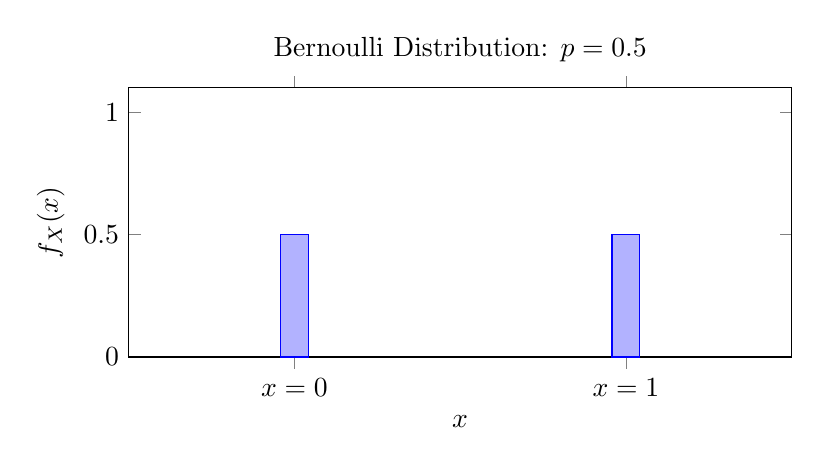
\begin{tikzpicture}
\begin{axis}[
    width=10cm,
    height=5cm,
    ybar,
    bar width=10pt,
    ymin=0,
    ymax=1.1,
    xmin=-0.5,
    xmax=1.5,
    xtick={0,1},
    xticklabels={$x=0$, $x=1$},
    xlabel={$x$},
    ylabel={$f_X(x)$},
    title={Bernoulli Distribution: $p = 0.5$},
    % ymajorgrids=true,
    % grid style=dashed
]
\addplot+[blue, fill=blue!30] coordinates {(0,0.5) (1,0.5)};
\end{axis}
\end{tikzpicture}
\end{center}

\subsection{Mean and Variance of the Bernoulli Distribution}

Let $X \sim \text{Bernoulli}(p)$.
\begin{itemize}
    \item \textbf{Mean}:
\[
\mathbb{E}(X) = \sum_{x} x \cdot P(X = x) = 0 \cdot (1 - p) + 1 \cdot p = p
\]
\begin{textbox}
    \[
\mathbb{E}(X) = p
\]
\end{textbox}

The mean of a Bernoulli distribution is simply the probability of success, $p$.


\item \textbf{Variance}:
\[
\text{Var}(X) = \mathbb{E}[X^2] - (\mathbb{E}(X))^2
\]

Note that for a Bernoulli variable, $X^2 = X$ (since $X$ is either 0 or 1), so:
\[
\mathbb{E}[X^2] = \mathbb{E}(X) = p
\]
\[
\text{Var}(X) = p - p^2 = p(1 - p)
\]
\begin{textbox}
    \[
\text{Var}(X) = p(1 - p)
\]
\end{textbox}

The variance of a Bernoulli distribution depends on both the probability of success and failure. It is maximum when $p = 0.5$.
\end{itemize}

\section{Binomial Distribution}

The {Binomial distribution} arises from repeating a Bernoulli trial independently $n$ number of times, where each trial has the same probability of success $p$.


Let $X$ denote the number of successes in $n$ independent Bernoulli trials, where each trial has two outcomes: {success} (with probability $p$) and {failure} (with probability $1 - p$).
Then the discrete random variable $X$ follows a \textbf{Binomial distribution} with parameters $n$ and $p$, written as:
\[
X \sim \text{Binomial}(n, p)
\]

The probability mass function (PMF) of $X$ is given by:
\begin{textbox}
\[
p_X(x) = P(X = x) =
\begin{cases}
\binom{n}{x} p^x (1 - p)^{n - x}, & \text{for } x = 0, 1, 2, \ldots, n \\
0, & \text{otherwise}
\end{cases}
\]

\end{textbox}

To derive this PMF, consider the following:

\begin{itemize}
    \item We want the probability of getting exactly $x$ successes (and hence $n - x$ failures) in $n$ trials.
    \item Each specific sequence of outcomes with $x$ successes and $n - x$ failures has probability:
    \[
    p^x (1 - p)^{n - x}
    \]
    because of the independence of trials.
    \item However, there are multiple ways (distinct sequences) to arrange $x$ successes among $n$ trials. The number of such arrangements is given by the binomial coefficient:
    \[
    \binom{n}{x} = \frac{n!}{x!(n - x)!}
    \]
\end{itemize}

Thus, the total probability of getting exactly $x$ successes is:
\[
P(X = x) = \binom{n}{x} p^x (1 - p)^{n - x}
\]

This expression defines the PMF of the binomial distribution.

\begin{textbox}
    A Binomial random variable is the sum of independent Bernoulli random variables i.e. if $$X=\sum_{i=1}^{n} X_i, \text{ with } X_i\sim \text{Bernoulli}(p)$$ for all $i = 1,2,\dots, n$,
    then, $$X\sim \text{Binomial}(n, p)$$
\end{textbox}

\vspace{2mm}

\textbf{Example}: Suppose a fair coin (with $p = 0.5$) is tossed 4 times. Let $X$ be the number of heads observed. Then $X \sim \text{Binomial}(4, 0.5)$. The PMF is:

\[
p_X(x) = \binom{4}{x} \times (0.5)^x \times (0.5)^{4 - x}, \quad x = 0, 1, 2, 3, 4
\]

Evaluating:
\[
\begin{aligned}
p_X(0) &= \binom{4}{0} \times (0.5)^0 \times (0.5)^4 = 1 \times 1 \times 0.0625 = 0.0625 \\
p_X(1) &= \binom{4}{1} \times (0.5)^1 \times (0.5)^3 = 4 \times 0.5 \times 0.125 = 0.25 \\
p_X(2) &= \binom{4}{2} \times (0.5)^2 \times (0.5)^2 = 6 \times 0.25 \times 0.25 = 0.375 \\
p_X(3) &= \binom{4}{3} \times (0.5)^3 \times (0.5)^1 = 4 \times 0.125 \times 0.5 = 0.25 \\
p_X(4) &= \binom{4}{4} \times (0.5)^4 \times (0.5)^0 = 1 \times 0.0625 \times 1 = 0.0625
\end{aligned}
\]


\begin{center}
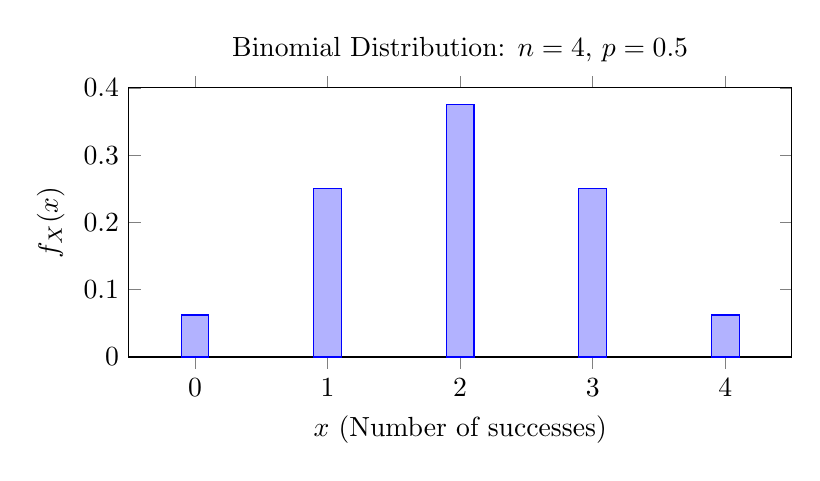
\begin{tikzpicture}
\begin{axis}[
    width=10cm,
    height=5cm,
    ybar,
    bar width=10pt,
    ymin=0,
    ymax=0.4,
    xmin=-0.5,
    xmax=4.5,
    xtick={0,1,2,3,4},
    xlabel={$x$ (Number of successes)},
    ylabel={$f_X(x)$},
    title={Binomial Distribution: $n = 4$, $p = 0.5$},
    % ymajorgrids=true,
    % grid style=dashed
]
\addplot+[blue, fill=blue!30] coordinates {
    (0,0.0625)
    (1,0.25)
    (2,0.375)
    (3,0.25)
    (4,0.0625)
};
\end{axis}
\end{tikzpicture}
\end{center}

\textbf{Example:} A fair six-sided die is rolled 8 times. What is the probability that the number 3 or 4 appears exactly 3 times?

Let a `success' be defined as getting either a 3 or a 4 in a single roll. The probability of success on one roll is:

\[
p = P(3 \text{ or } 4) = \frac{1}{6} + \frac{1}{6} = \frac{2}{6} = \frac{1}{3}
\]

Let $X$ be the number of successes (i.e., times 3 or 4 occurs) in $n = 8$ independent die rolls. Then $X$ follows a binomial distribution:

\[
X \sim \text{Binomial}\left(n =8, p = \frac{1}{3}\right)
\]

We want to find the probability three successes i.e. $X = 3$:

\[
P(X = 3) = \binom{8}{3} \times \left( \frac{1}{3} \right)^3 \times \left( \frac{2}{3} \right)^5
\]

Now, compute the values:

\[
\binom{8}{3} = 56, \quad \left( \frac{1}{3} \right)^3 = \frac{1}{27}, \quad \left( \frac{2}{3} \right)^5 = \frac{32}{243}
\]

\[
P(X = 3) = 56 \times \frac{1}{27} \times \frac{32}{243} = \frac{1792}{6561} \approx 0.273
\]

\subsection{Mean and Variance of the Binomial Distribution}

Let $X \sim \text{Binomial}(n, p)$.

\begin{itemize}
    \item \textbf{Mean}:

    Consider $X$ as the sum of $n$ independent Bernoulli random variables:
    \[
    X = X_1 + X_2 + \cdots + X_n, \quad \text{where } X_i \sim \text{Bernoulli}(p)
    \]

    Since expectation is linear:
    \[
    \mathbb{E}(X) = \mathbb{E}[X_1 + X_2 + \cdots + X_n] = \mathbb{E}[X_1] + \mathbb{E}[X_2] + \cdots + \mathbb{E}[X_n]
    \]

    Each $X_i$ has expected value $p$, so:
    \begin{textbox}
        \[
    \mathbb{E}(X) = n \cdot p
    \]
    \end{textbox}

    Thus on average, we can expect $n \cdot p$ successes in $n$ trials.

    \item \textbf{Variance}:

    Since the $X_i$'s are independent:
    \[
    \text{Var}(X) = \text{Var}(X_1 + X_2 + \cdots + X_n) = \text{Var}(X_1) + \text{Var}(X_2) + \cdots + \text{Var}(X_n)
    \]

    Each $X_i$ is Bernoulli with variance $p(1 - p)$, so:
    \begin{textbox}
        \[
    \text{Var}(X) = n \cdot p(1 - p)
    \]
    \end{textbox}

    The variance increases with the number of trials and depends on both the probability of success and failure.
\end{itemize}

\section{Poisson Distribution}

The {Poisson distribution} is commonly used to model the number of occurrences of an event in a fixed interval of time or space, under the following assumptions:
\begin{itemize}
    \item Events occur independently.
    \item The average rate ($\lambda$) of occurrence is constant over the interval.
    \item Two events cannot occur at exactly the same instant.
\end{itemize}

Let $X$ denote the number of such events occurring in a fixed interval with an average value $\lambda$, then we say that the discrete random variable $X$ follows a \textbf{Poisson distribution} with parameter $\lambda > 0$, and write:
\[
X \sim \text{Poisson}(\lambda)
\]

The probability mass function (PMF) of $X$ is given by:
\begin{textbox}
\[
p_X(x) = P(X = x) =
\begin{cases}
\displaystyle \frac{e^{-\lambda} \lambda^x}{x!}, & \text{for } x = 0, 1, 2, \ldots \\
0, & \text{otherwise}
\end{cases}
\]
\end{textbox}

\textbf{Example:} Suppose a call center receives an average of 4 calls per minute. What is the probability that exactly 2 calls are received in a particular minute?

Let $X$ be the number of calls per minute. Then:
\[
X \sim \text{Poisson}(\lambda = 4)
\]
We want to find $P(X = 2)$:
\[
P(X = 2) = \frac{e^{-4} \cdot 4^2}{2!} = \frac{e^{-4} \cdot 16}{2} = 8e^{-4} \approx 0.1465
\]

\begin{center}
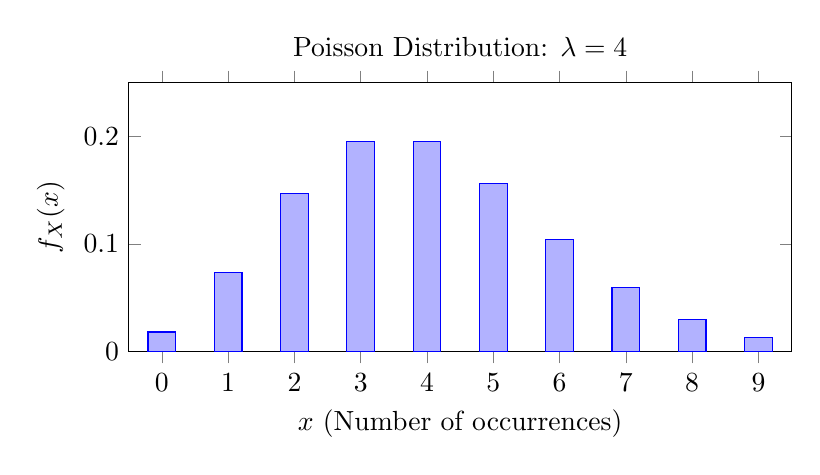
\begin{tikzpicture}
\begin{axis}[
    width=10cm,
    height=5cm,
    ybar,
    bar width=10pt,
    ymin=0,
    ymax=0.25,
    xmin=-0.5,
    xmax=9.5,
    xtick={0,1,2,3,4,5,6,7,8,9},
    xlabel={$x$ (Number of occurrences)},
    ylabel={$f_X(x)$},
    title={Poisson Distribution: $\lambda = 4$},
]
\addplot+[blue, fill=blue!30] coordinates {
    (0,0.0183)
    (1,0.0733)
    (2,0.1465)
    (3,0.1954)
    (4,0.1954)
    (5,0.1563)
    (6,0.1042)
    (7,0.0595)
    (8,0.0297)
    (9,0.0132)
};
\end{axis}
\end{tikzpicture}
\end{center}

\textbf{Example}: In a football league, the number of goals scored by a team in a match is modeled using a Poisson distribution. Based on historical performance, Team A scores an average of $2.1$ goals per match.

\begin{enumerate}
    \item What is the probability that Team A scores exactly 3 goals in an upcoming match?
    \item What is the probability that Team A scores fewer than 2 goals?
    \item What is the probability that Team A scores at least 2 goals?
    \item What is the expected number of goals Team A will score over their next 5 matches?
\end{enumerate}

The Poisson probability mass function (PMF) is given by:
\[
f_X(x) = P(X=x)= \frac{e^{-\lambda} \lambda^x}{x!}
\quad \text{where } \lambda = 2.1, \quad x = 0, 1, 2, \dots
\]

\begin{enumerate}
    \item {Probability that Team A scores exactly 3 goals:}
    \[
    f_X(3)  = \frac{e^{-2.1} \cdot 2.1^3}{3!}
    = \frac{e^{-2.1} \cdot 9.261}{6}
    \approx \frac{0.1225 \cdot 9.261}{6}
    \approx 0.189
    \]

    \item {Probability that Team A scores fewer than 2 goals:}
    \[
    P(X < 2) = {P}(X = 0) + {P}(X = 1) = f_X(0) + f_X(1)
    \]
    \[
    f_X(0) = e^{-2.1} \approx 0.1225, \quad
    f_X(1) = \frac{e^{-2.1} \cdot 2.1}{1!} \approx 0.2573
    \]
    \[
    P(X < 2) \approx 0.1225 + 0.2573 = 0.3798
    \]

    \item {Probability that Team A scores at least 2 goals:}
    \[
    P(X \geq 2) = 1 - P(X < 2) = 1 - 0.3798 = 0.6202
    \]

    \item {Expected number of goals over 5 matches:}
    \[
    5 \times \mathbb{E}(X) = 5 \times \lambda = 5 \times 2.1 = 10.5
    \]
\end{enumerate}

\begin{textbox}
\textbf{Theorem}: The Poisson distribution can be obtained as the limiting distribution of the Binomial distribution when the number of trials \( n \to \infty \), the success probability \( p \to 0\), while the expected number of successes \( \lambda = np \) remains constant. Formally,
\[
\text{Binomial}(n, p) \longrightarrow \text{Poisson}(\lambda) \quad \text{as } n \to \infty, p \to 0 \text{ such that } np = \lambda (\text{constant})
\]
\end{textbox}

\textbf{Proof}: Let \( X \sim \text{Binomial}(n, p) \). The probability mass function (PMF) is:
\[
p_X(k) = \binom{n}{k} p^x (1 - p)^{n-x}, \quad x = 0, 1, 2, \ldots, n.
\]

We assume \( n \to \infty \) and \( p \to 0 \) such that the product \( \lambda = np \) remains fixed and finite. We can write the binomial coefficient as:
\begin{align*}
    \binom{n}{x} &= \frac{n (n-1) \cdots (n-x+1)}{x!} \\
    &= \frac{n^k}{x!} \left(1 - \frac{1}{n}\right)\left(1 - \frac{2}{n}\right) \dots \left(1 - \frac{x-1}{n}\right)
\end{align*}

As \( n \to \infty \), each of the product terms approaches 1:
Thus,
\[
\binom{n}{x} \to \frac{n^x}{x!}
\]

Now using this limiting expression of $\binom{n}{x}$ and replacing \( p \) with \( \dfrac{\lambda}{n} \), we get:
\[
p_X(x) \approx \frac{n^x}{x!} \left(\frac{\lambda}{n}\right)^x \left(1 - \frac{\lambda}{n}\right)^{n-x} = \frac{\lambda^x}{x!} \left(1 - \frac{\lambda}{n}\right)^{n-x}
\]

Rewrite the last term as:
\[
\left(1 - \frac{\lambda}{n}\right)^{n-x} = \left(1 - \frac{\lambda}{n}\right)^n \left(1 - \frac{\lambda}{n}\right)^{-x}
\]

As \( n \to \infty \),
\[
\left(1 - \frac{\lambda}{n}\right)^n \to e^{-\lambda}
\quad \text{and} \quad
\left(1 - \frac{\lambda}{n}\right)^{-x} \to 1,
\]
since \( x \) is fixed.


Therefore in the limit \( n \to \infty \):
\[
\lim_{n \to \infty} p_X(x) = \frac{\lambda^x}{x!} e^{-\lambda} \cdot 1 = \frac{e^{-\lambda} \lambda^x}{x!}
\]

This matches the PMF of the Poisson distribution with parameter \( \lambda \).

\hfill\(\blacksquare\)

\subsection{Mean and Variance of the Poisson Distribution}

Let $X \sim \text{Poisson}(\lambda)$.

\begin{itemize}
    \item \textbf{Mean}:
    % \begin{align*}
    %     \mathbb{E}(X) &= \sum_{x=0}^{\infty} x \cdot P(X = x) = \sum_{x=0}^{\infty} x \cdot \frac{e^{-\lambda} \lambda^x}{x!} \\
    %     &=\frac{e^{-\lambda}\left(0+1\times\frac{\lambda^1}{1}+2\times\frac{\lambda^2}{2}+\dots \right)
    % \end{align*}
    \begin{align*}
\mathbb{E}(X) &= \sum_{x=0}^{\infty} x \cdot P(X = x) = \sum_{x=0}^{\infty} x \cdot \frac{e^{-\lambda} \lambda^x}{x!} \\
&= e^{-\lambda} \sum_{x=1}^{\infty} x \cdot \frac{\lambda^x}{x!} = e^{-\lambda} \sum_{x=1}^{\infty} \frac{\lambda^x}{(x-1)!} \\
&= e^{-\lambda} \cdot \lambda \sum_{x=1}^{\infty} \frac{\lambda^{x-1}}{(x-1)!} \\
&= \lambda \cdot e^{-\lambda} \sum_{k=0}^{\infty} \frac{\lambda^k}{k!} \quad \text{(let } k = x - 1 \text{)} \\
&= \lambda \cdot e^{-\lambda} \cdot e^{\lambda} = \lambda
\end{align*}

    \begin{textbox}
        \[
    \mathbb{E}(X) = \lambda
    \]
    \end{textbox}

    \item \textbf{Variance}:
    \[
    \text{Var}(X) = \mathbb{E}[X^2] - (\mathbb{E}(X))^2
    \]

    First we evaluate
\[
\mathbb{E}[X^2] = \sum_{x=0}^{\infty} x^2 \cdot \frac{e^{-\lambda} \lambda^x}{x!}
\]

We use the identity \(x^2 = x(x - 1) + x\), giving:
\[
\mathbb{E}[X^2] = \sum_{x=0}^{\infty} \left[x(x - 1) + x\right] \cdot \frac{e^{-\lambda} \lambda^x}{x!}
= e^{-\lambda} \left( \sum_{x=0}^{\infty} \frac{x(x-1) \lambda^x}{x!} + \sum_{x=0}^{\infty} \frac{x \lambda^x}{x!} \right)
\]

We compute each sum:
\[
\sum_{x=0}^{\infty} \frac{x(x-1) \lambda^x}{x!} =\sum_{x=2}^{\infty} \frac{\lambda^x}{(x-2)!}=\lambda^2\sum_{j=0}^{\infty} \frac{\lambda^j}{j!} =\lambda^2 e^{\lambda}
\]

And,
$$\sum_{x=0}^{\infty} \frac{x \lambda^x}{x!} = =\sum_{x=1}^{\infty} \frac{\lambda^x}{(x-1)!}=\lambda\sum_{j=0}^{\infty} \frac{\lambda^j}{j!} =\lambda e^{\lambda}$$

Therefore,
\[
\mathbb{E}[X^2] = e^{-\lambda} \left( \lambda^2 e^{\lambda} + \lambda e^{\lambda} \right) = \lambda^2 + \lambda
\]

  Therefore:
    \[
    \text{Var}(X) = (\lambda + \lambda^2) - \lambda^2 = \lambda
    \]

    \begin{textbox}
        \[
    \text{Var}(X) = \lambda
    \]
    \end{textbox}

    \vspace{3mm}

    There is an alternative way of calculating the variance using the moment generating function (MGF).

    The moment generating function (MGF) of \( X \) is defined as:
    \[
M_X(t) = \mathbb{E}[e^{tX}] = \sum_{k=0}^{\infty} e^{t x} \cdot \frac{e^{-\lambda} \lambda^x}{x!}
\]

Factor out the constant \( e^{-\lambda} \):
\[
M_X(t) = e^{-\lambda} \sum_{x=0}^{\infty} \frac{(\lambda e^t)^x}{x!}
\]

This is the exponential series:
\[
\sum_{x=0}^{\infty} \frac{(\lambda e^t)^x}{x!} = e^{\lambda e^t}
\]

Therefore,
\[
M_X(t) = e^{-\lambda} \cdot e^{\lambda e^t} = e^{\lambda(e^t - 1)}
\]

To compute the variance \( \mathrm{Var}(X) \), we use the identity:
\[
\mathrm{Var}(X) = \mathbb{E}[X^2] - (\mathbb{E}(X))^2 = \mu_2' - \mu^2 = \mu_2' - (\mu_1')^2
\]

We compute the first and second raw moments using derivatives of the MGF:

\underline{First raw moment (mean):}
\[
M_X'(t) = \frac{d}{dt} \left[ e^{\lambda(e^t - 1)} \right]
= \lambda e^t \cdot e^{\lambda(e^t - 1)}
\]

Evaluating at \( t = 0 \):
\[
\mu_1' = M_X'(0) = \lambda \cdot 1 \cdot e^{\lambda(1 - 1)} = \lambda
\]

\underline{Second raw moment:}
\[
M_X''(t) = \frac{d}{dt} \left[ \lambda e^t \cdot e^{\lambda(e^t - 1)} \right]
= \lambda e^t \left[ \lambda e^t \cdot e^{\lambda(e^t - 1)} + e^{\lambda(e^t - 1)} \right]
= \lambda e^t e^{\lambda(e^t - 1)} (\lambda e^t + 1)
\]

Evaluating at \( t = 0 \):
\[
\mu_2' = M_X''(0) = \lambda \cdot 1 \cdot 1 \cdot (\lambda \cdot 1 + 1) = \lambda(\lambda + 1) = \lambda^2 + \lambda
\]

\underline{Now compute the variance:}
\[
\mathrm{Var}(X) = \mu_2' - (\mu_1')^2 = (\lambda^2 + \lambda) - \lambda^2 = \lambda
\]
\end{itemize}

% \textbf{Remark:} Because the mean and variance are equal, Poisson models are particularly useful for count data with this characteristic. If variance is significantly greater than the mean, other models (e.g., Negative Binomial) may be more appropriate.

\section{Uniform Distribution}

The Uniform distribution is the simplest continuous probability distribution, where all outcomes in a given interval are equally likely.

Let $X$ be a continuous random variable that is uniformly distributed on the interval $[a, b]$, where $a < b$. This means that $X$ has constant probability density over this interval. We write:

\[
X \sim \text{Uniform}(a, b)
\]

The probability density function (PDF) of $X$ is given by:

\begin{textbox}
\[
f_X(x) =
\begin{cases}
\frac{1}{b - a}, & a \le x \le b \\
0, & \text{otherwise}
\end{cases}
\]
\end{textbox}

That is, the probability density is constant between $a$ and $b$, and zero elsewhere. The total area under the curve is 1, ensuring it satisfies the definition of a probability density function.

A continuous uniform distribution models situations where every outcome in an interval is equally likely—such as the exact time (within an hour) a bus arrives, or the position of a point randomly placed on a stick.

\vspace{2mm}
\textbf{Example:} Suppose that a variable $X$ is uniformly distributed over the interval $[2, 5]$. Then:

\[
f_X(x) =
\begin{cases}
\frac{1}{5 - 2} = \frac{1}{3}, & 2 \le x \le 5 \\
0, & \text{otherwise}
\end{cases}
\]

We can compute probabilities over intervals by integrating the density. For example:

\[
P(3 \le X \le 4) = \int_{3}^{4} \frac{1}{3} dx = \frac{1}{3}(4 - 3) = \frac{1}{3}
\]

\begin{center}
\begin{tikzpicture}
\begin{axis}[
    width=10cm,
    height=5cm,
    ymin=0, ymax=0.5,
    xmin=1, xmax=6,
    axis lines=left,
    xlabel={$x$},
    ylabel={$f_X(x)$},
    title={Uniform Distribution: $a = 2$, $b = 5$},
    xtick={2,3,4,5},
    ytick={0.33},
    yticklabels={$1/3$},
    domain=2:5,
    samples=2
]
% \addplot+[blue, thick, fill=blue!30, draw=none, domain=3:4] {1/3} \closedcycle;
% \addplot[blue, thick] {1/3};
\addplot[
    blue,
    very thick
] coordinates {
    (0,0)
    (2,0)
};
\addplot[
    blue,
    dotted
] coordinates {
    (2,0)
    (2,1/3)
};
\addplot[
    blue,
    very thick
] coordinates {
    (2,1/3)
    (5,1/3)
};
\addplot[
    blue,
    dotted
] coordinates {
    (5,1/3)
    (5,0)
};
\addplot[
    blue,
    very thick
] coordinates {
    (5,0)
    (6,0)
};
\end{axis}
\end{tikzpicture}
\end{center}

\subsection{Mean and Variance of the Uniform Distribution}

Let $X \sim \text{Uniform}(a, b)$.

\begin{itemize}
    \item \textbf{Mean}:
\begin{align*}
\mathbb{E}(X) &= \int_a^b x \cdot \frac{1}{b - a} \, dx
= \frac{1}{b - a} \int_a^b x \, dx \\
&= \frac{1}{b - a} \cdot \left[ \frac{x^2}{2} \right]_a^b
= \frac{1}{b - a} \cdot \left( \frac{b^2 - a^2}{2} \right) \\
&= \frac{1}{b - a} \cdot \frac{(b - a)(b + a)}{2}
= \frac{a + b}{2}
\end{align*}

    \begin{textbox}
    \[
    \mathbb{E}(X) = \frac{a + b}{2}
    \]
    \end{textbox}

    \item \textbf{Variance}:
    \[
    \text{Var}(X) = \mathbb{E}(X^2) - [\mathbb{E}(X)]^2
    \]
    with:
    \[
    \mathbb{E}(X^2) = \int_a^b x^2 \cdot \frac{1}{b - a} dx = \frac{1}{b - a} \left[\dfrac{x^3}{3}\right]_a^b= \frac{b^3 - a^3}{3(b - a)}
    \]
    \begin{textbox}
    \[
    \text{Var}(X) = \frac{(b - a)^2}{12}
    \]
    \end{textbox}
\end{itemize}

\vspace{2mm}

\textbf{Example:} For $X \sim \text{Uniform}(2, 5)$:

\[
\mathbb{E}(X) = \frac{2 + 5}{2} = 3.5, \quad \text{Var}(X) = \frac{(5 - 2)^2}{12} = \frac{9}{12} = 0.75
\]


\section{Normal Distribution}

The \textbf{Normal distribution}, also known as the \textbf{Gaussian distribution}, is one of the most important continuous probability distributions in statistics. It models many naturally occurring phenomena such as heights, test scores, measurement errors, etc. When a continuous random variable $X$ is said to follow a {Normal distribution} with parameter $\mu$ and $\sigma^2$, we denote it as:
\[
X \sim \mathcal{N}(\mu, \sigma^2)
\]

The probability density function (PDF) of the Normal distribution is given by:
\begin{textbox}
\[
f_X(x) = \frac{1}{\sqrt{2\pi\sigma^2}} \exp\left( -\frac{(x - \mu)^2}{2\sigma^2} \right), \quad \text{for } -\infty \leq x \leq \infty
\]
\end{textbox}

The distribution is completely determined by the parameters $\mu$ and $\sigma^2$. In future, we will show that the mean and variance of the normal distribution are those parameters $\mu$ and $\sigma^2$ respectively.

\textbf{Example}: Let $X \sim \mathcal{N}(2, 1^2)$, i.e., a normal distribution with mean $\mu = 2$ and standard deviation $\sigma = 1$.
We want to compute the value of the probability density function (PDF) at $x = 1.5$.

The PDF of a normal distribution is:
\[
f_X(x) = \frac{1}{\sigma\sqrt{2\pi }} \exp\left( -\frac{(x - \mu)^2}{2\sigma^2} \right)
\]

Substitute $\mu = 2$, $\sigma = 1$, and $x = 1.5$:
\[
f_X(1.5) = \frac{1}{\sqrt{2\pi}} \exp\left( -\frac{(1.5 - 2)^2}{2} \right)
= \frac{1}{\sqrt{2\pi}} \exp\left( -\frac{0.25}{2} \right)
= \frac{1}{\sqrt{2\pi}} \exp(-0.125)
\]

Now compute numerically:
\[
\frac{1}{\sqrt{2\pi}} \approx 0.3989, \quad \exp(-0.125) \approx 0.8825
\]

\[
f_X(1.5) \approx 0.3989 \times 0.8825 \approx 0.3521
\]

The plot of the PDF of $X \sim \mathcal{N}(2,1)$ is shown in the figure below:

\begin{center}
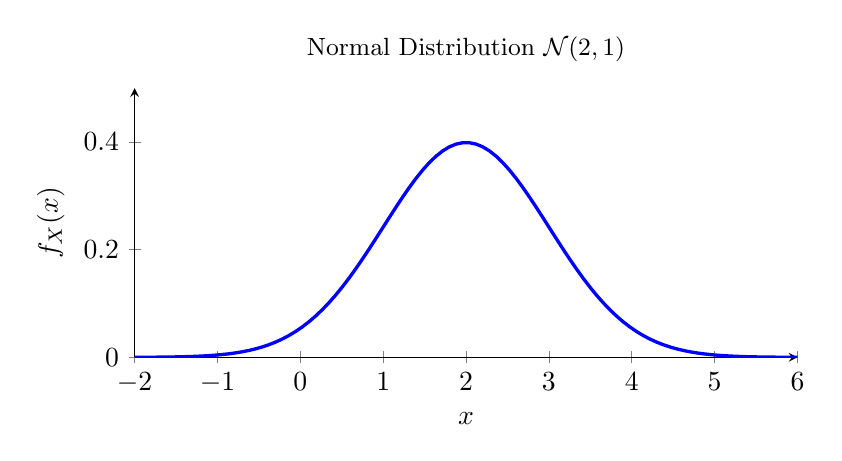
\begin{tikzpicture}
\begin{axis}[
    no markers, domain=-2:6, samples=100,
    axis lines=left,
    xlabel=$x$, ylabel={$f_X(x)$},
    height=5cm, width=10cm,
    ymin=0, ymax=0.5,
    xmin=-2, xmax=6,
    title={\small Normal Distribution $\mathcal{N}(2,1)$}
]
\addplot [very thick,blue] {1/sqrt(2*pi)*exp(-(x-2)^2/2)};
\end{axis}
\end{tikzpicture}
\end{center}

\subsection{Mean and Variance of the Normal Distribution}

Let $X \sim \mathcal{N}(\mu, \sigma^2)$.

\begin{itemize}
    \item \textbf{Mean}:

    \begin{align*}
    \mathbb{E}[X]
    &= \int_{-\infty}^{\infty} x \; f_X(x)\,dx
    = \int_{-\infty}^{\infty} x \;\frac{1}{\sqrt{2\pi}\,\sigma}
    \exp\!\biggl(-\frac{(x-\mu)^2}{2\sigma^2}\biggr)\,dx \\[6pt]
    %
    \text{Let } u &= \frac{x - \mu}{\sigma}
    \quad\Longrightarrow\quad
    x = \sigma u + \mu,
    \quad dx = \sigma\,du, \\[3pt]
    %
    \mathbb{E}[X] &= \int_{-\infty}^{\infty}
    (\sigma u + \mu)\;
    \frac{1}{\sqrt{2\pi}\,\sigma}
    \exp\!\bigl(-\tfrac{u^2}{2}\bigr)\;\sigma\,du \\[6pt]
    %
    &= \int_{-\infty}^{\infty}
    (\sigma u + \mu)\;
    \frac{1}{\sqrt{2\pi}}
    \exp\!\bigl(-\tfrac{u^2}{2}\bigr)\;du \\[6pt]
    %
    &= \underbrace{\int_{-\infty}^{\infty}
    \sigma u \;\frac{1}{\sqrt{2\pi}}
    e^{-u^2/2}\,du}_{=\,0\;\text{(odd integrand)}}
    \;+\;
    \mu \int_{-\infty}^{\infty}
    \frac{1}{\sqrt{2\pi}}
    e^{-u^2/2}\,du \\[6pt]
    %
    &= 0 \;+\; \mu \cdot 1
    \;=\; \mu.
    \end{align*}

    \begin{textbox}
        \[
        \mathbb{E}(X) = \mu
        \]
        \end{textbox}


    \item \textbf{Variance}:
    \begin{align*}
    \operatorname{Var}(X)
    &= \mathbb{E}\bigl[(X - \mu)^2\bigr]
    = \int_{-\infty}^{\infty} (x - \mu)^2 \; f_X(x)\,dx \\
    &= \int_{-\infty}^{\infty} (x - \mu)^2 \;\frac{1}{\sqrt{2\pi}\,\sigma}
    \exp\!\Bigl(-\frac{(x-\mu)^2}{2\sigma^2}\Bigr)\,dx \\[6pt]
    %
    \text{Let } u &= \frac{x - \mu}{\sigma}
    \quad\Longrightarrow\quad
    x - \mu = \sigma u,
    \quad dx = \sigma\,du, \\[3pt]
    %
    \operatorname{Var}(X)&= \int_{-\infty}^{\infty}
    (\sigma u)^2 \;
    \frac{1}{\sqrt{2\pi}\,\sigma}
    \exp\!\bigl(-\tfrac{u^2}{2}\bigr)\;\sigma\,du \\[6pt]
    %
    &= \int_{-\infty}^{\infty}
    \sigma^2 u^2 \;
    \frac{1}{\sqrt{2\pi}}
    \exp\!\bigl(-\tfrac{u^2}{2}\bigr)\;du \\[6pt]
    %
    &= \sigma^2 \underbrace{\int_{-\infty}^{\infty}
            u^2 \;\frac{1}{\sqrt{2\pi}} e^{-u^2/2}\,du}_{\text{We need to prove this equals 1}}\\
    &= \frac{\sigma^2}{\sqrt{2\pi}} \int_{-\infty}^{\infty} u^2\,e^{-u^2/2}\,du\\
    &= \frac{2\sigma^2}{\sqrt{2\pi}} \int_{0}^{\infty} u^2\,e^{-u^2/2}\,du\
    \end{align*}

    Now, using the Gamma integral formula\footnote{Gamma integral formula:
    $$\int_{0}^{\infty} x^n e^{-a x^2}dx
         = \tfrac12\,a^{-\frac{n+1}{2}}\Gamma\!\bigl(\tfrac{n+1}{2}\bigr)$$
         $$\Gamma(n+1) = n\Gamma(n), \quad \Gamma(\tfrac12) = \sqrt{\pi}$$
         },
    \begin{align*}
    \int_{0}^{\infty} u^2\,e^{-u^2/2}\,du
    &= \frac{1}{2}\,\Bigl(\tfrac12\Bigr)^{-\frac{3}{2}}
       \,\Gamma\!\Bigl(\tfrac{3}{2}\Bigr)\\
    &= \frac{1}{2}\,\cdot 2^{3/2}\,\cdot \frac{1}{2}\sqrt{\pi}
    &&\bigl((\tfrac12)^{-3/2}=2^{3/2},\ \Gamma(\tfrac32)=\tfrac12\Gamma(\tfrac12) = \tfrac12\sqrt\pi\bigr)\\
    &= \frac{\sqrt{2\pi}}{2}
    \end{align*}

    Therefore,
    \[
    \text{Var}(X) = \sigma^2 \frac{2}{\sqrt{2\pi}} \times \frac{\sqrt{2\pi}}{2}
      = \sigma^2
    \]

        \begin{textbox}
        \[
        \text{Var}(X) = \sigma^2
        \]
        \end{textbox}
\end{itemize}

\subsection{Moment Generating Function of the Normal Distribution}

Let \( X \sim N(\mu, \sigma^2) \) be a normal random variable with mean \(\mu\) and variance \(\sigma^2\). The moment generating function (MGF) of \(X\) is defined as
\begin{align*}
M_X(t) = \mathbb{E}\left( e^{tX}\right)  &= \int_{-\infty}^{\infty} e^{tx} \frac{1}{\sqrt{2\pi\sigma^2}} \exp\left(-\frac{(x-\mu)^2}{2\sigma^2}\right) \, dx \\
&=\frac{1}{\sqrt{2\pi\sigma^2}} \int_{-\infty}^{\infty} \exp\left(tx - \frac{(x-\mu)^2}{2\sigma^2}\right) dx
\end{align*}

Rewrite the exponent as:
\begin{align*}
tx - \frac{(x-\mu)^2}{2\sigma^2} &= -\frac{1}{2\sigma^2} (x-\mu)^2 + tx\\
&=-\frac{1}{2\sigma^2} (x^2 - 2\mu x + \mu^2) + t x\\
&=-\frac{x^2}{2\sigma^2} + \frac{\mu x}{\sigma^2} - \frac{\mu^2}{2\sigma^2} + t x \\
&=-\frac{x^2}{2\sigma^2} + \left(\frac{\mu}{\sigma^2} + t\right) x - \frac{\mu^2}{2\sigma^2} \quad (\text{Group terms involving } x)\\
&=-\frac{1}{2\sigma^2} \left[x^2 - 2 (\mu + \sigma^2 t) x \right] - \frac{\mu^2}{2\sigma^2}\\
&=-\frac{1}{2\sigma^2} \left[(x - (\mu + \sigma^2 t))^2 - (\mu + \sigma^2 t)^2 \right] - \frac{\mu^2}{2\sigma^2}\\
&=-\frac{(x - (\mu + \sigma^2 t))^2}{2\sigma^2} + \frac{(\mu + \sigma^2 t)^2}{2\sigma^2} - \frac{\mu^2}{2\sigma^2}\\
&=-\frac{(x - (\mu + \sigma^2 t))^2}{2\sigma^2} + \frac{\mu^2 + 2 \mu \sigma^2 t + \sigma^4 t^2 - \mu^2}{2 \sigma^2}\\
&=-\frac{(x - (\mu + \sigma^2 t))^2}{2\sigma^2} + \mu t + \frac{1}{2} \sigma^2 t^2
\end{align*}

Substitute this back into the integral for the MGF:
\[
M_X(t) = \frac{1}{\sqrt{2 \pi \sigma^2}} \int_{-\infty}^\infty \exp\left(-\frac{(x - (\mu + \sigma^2 t))^2}{2\sigma^2} + \mu t + \frac{1}{2} \sigma^2 t^2 \right) dx
\]

Factor out terms that do not depend on \(x\):
\[
M_X(t) = \exp\left(\mu t + \frac{1}{2} \sigma^2 t^2\right) \cdot \underbrace{\frac{1}{\sqrt{2 \pi \sigma^2}} \int_{-\infty}^\infty \exp\left(-\frac{(x - (\mu + \sigma^2 t))^2}{2\sigma^2}\right) dx}_{= 1}
\]

The integral is the integral of a normal pdf with mean \(\mu + \sigma^2 t\) and variance \(\sigma^2\), and is equal to 1.

Hence,

\begin{textbox}
\[
M_X(t) = \exp\left(\mu t + \frac{1}{2} \sigma^2 t^2 \right)
\]
\end{textbox}

This moment generating function exists for all real values of \(t\) and uniquely characterizes the normal distribution.



\subsection{Properties of the Normal Distribution}

\begin{enumerate}
  \item The \textbf{support} of a normal random variable \(X \sim N(\mu,\sigma^2)\) is the entire real line:
    \[
	(-\infty \leq X \leq\,+\infty)
    \]
    This reflects that, however unlikely, arbitrarily large positive or negative values can occur.

  \item The probability density function is perfectly \textbf{symmetric} about its mean \(\mu\) since,
    \[
      f_X(\mu + x_0) = f_X(\mu - x_0) =  \frac{1}{\sigma\sqrt{2\pi }} \exp\left( -\frac{x_0^2}{2\sigma^2} \right)
      \quad\forall\,x_0\in\mathbb{R}.
    \]
    As a result, the left and right tails of the distribution mirror each other.

  \item Since the distribution is symmetrical about $\mu$, its mean and median coincide.To get the mode, we need to calculate the peak point of the distribution.
  \begin{align*}
  f_X(x) &= \frac{1}{\sigma\sqrt{2\pi}} \exp\left( -\frac{(x-\mu)^2}{2\sigma^2}\right)  \\[6pt]
  \frac{d}{dx}f_X(x)
  &= \frac{1}{\sigma\sqrt{2\pi}} \exp\left( -\frac{(x-\mu)^2}{2\sigma^2}\right)
     \cdot \frac{d}{dx}\left( -\tfrac{(x-\mu)^2}{2\sigma^2}\right)  \\[6pt]
  &= f_X(x)\,\Bigl(-\tfrac{2(x-\mu)}{2\sigma^2}\Bigr)
  = -\frac{x-\mu}{\sigma^2}\,f_X(x)
  \end{align*}
  Setting the derivative to zero for a stationary point:
  \begin{align*}
  -\frac{x-\mu}{\sigma^2}\,f_X(x) = 0
  \quad &\Longrightarrow\quad x - \mu = 0 \\[4pt]
  &\Longrightarrow\quad x = \mu
  \end{align*}

  Now,
  \begin{align*}
  f_X''(x)
  &= -\frac{1}{\sigma^2}\,f_X(x)
     + \Bigl(-\frac{x-\mu}{\sigma^2}\Bigr)\,f_X'(x)
  \\
  &= -\frac{1}{\sigma^2}\,f_X(x)
     + \Bigl(-\frac{x-\mu}{\sigma^2}\Bigr)\Bigl(-\frac{x-\mu}{\sigma^2}f_X(x)\Bigr)
  \\
  &= -\frac{1}{\sigma^2}\,f_X(x)
     + \frac{(x-\mu)^2}{\sigma^4}\,f_X(x)
  \\
  &= \frac{(x-\mu)^2 - \sigma^2}{\sigma^4}\,f_X(x)
  \end{align*}
  Evaluating at the stationary point \(x=\mu\):
  \[
  f_X''(\mu)
  = \frac{(\mu-\mu)^2 - \sigma^2}{\sigma^4}\,f_X(\mu)
  = -\frac{1}{\sigma^2}\,f_X(\mu)
  < 0,
  \]

  Hence the peak (mode) of the normal density occurs at \(x=\mu\).
  \begin{textbox}
  For normal distribution, all measures of central tendency coincide:
      \[
        \text{Mean} = \text{Median} = \text{Mode} = \mu.
      \]
  \end{textbox}


  \item The normal distribution curve has two \textbf{points of inflection}\footnote{A \textbf{point of inflection} of a function $f(x)$ is a point $x = a$ such that
  \[
  f''(a) = 0,
  \]
  At the point of inflexion, the second derivative $f''(x)$ changes sign as $x$ passes through $a$, meaning the curve switches between concave‐up and concave‐down at $x = a$.} at a distance $\sigma$ on either side of $\mu$ i.e. at
    \[
      x = \mu \pm \sigma.
    \]
    At these points the second derivative of \(f_X(x)\) vanishes, marking the transition between “concave down” near the center and “concave up” in the tails. To show that let's take the second derivative of $f_X(x)$ and equate it to zero:
   \begin{align*}
   f_X''(x) &= \frac{(x-\mu)^2 - \sigma^2}{\sigma^4}\,f_X(x) = 0 \\
   &\Rightarrow (x-\mu)^2 = \sigma^2 \\
   &\Rightarrow x-\mu = \pm\sigma \\
   &\Rightarrow x = \mu \pm\sigma \\
   \end{align*}

  \item All odd central moments are zero (due to symmetry), and the even central moments have closed‐form expressions:
    \[
      E\bigl[(X-\mu)^{2n+1}\bigr] = 0,
      \qquad
      E\bigl[(X-\mu)^{2n}\bigr] = \sigma^{2n}\,(2n - 1)!!,
      \quad n = 1,2,\dots
    \]
    In particular, the variance is \(E[(X-\mu)^2]=\sigma^2\), and the fourth central moment is \(3\sigma^4\), etc.

   \item The kurtosis of normal distribution is 3. (prove it)

  \item A normal distribution \(X\sim N(\mu,\sigma^2)\) satisfies the following empirical rules:

  \begin{textbox}
  \textbf{Empirical Rule (68-95-99.7 Rule)}:
    \begin{itemize}
        \item About 68.27\% of the values lie within $\sigma$ of the mean ($\mu \pm \sigma$).
        \item About 95.45\% of the values lie within $2\sigma$ of the mean ($\mu \pm 2\sigma$).
        \item About 99.73\% of the values lie within $3\sigma$ of mean ($\mu \pm 3\sigma$).
    \end{itemize}
  \end{textbox}

  \begin{center}
    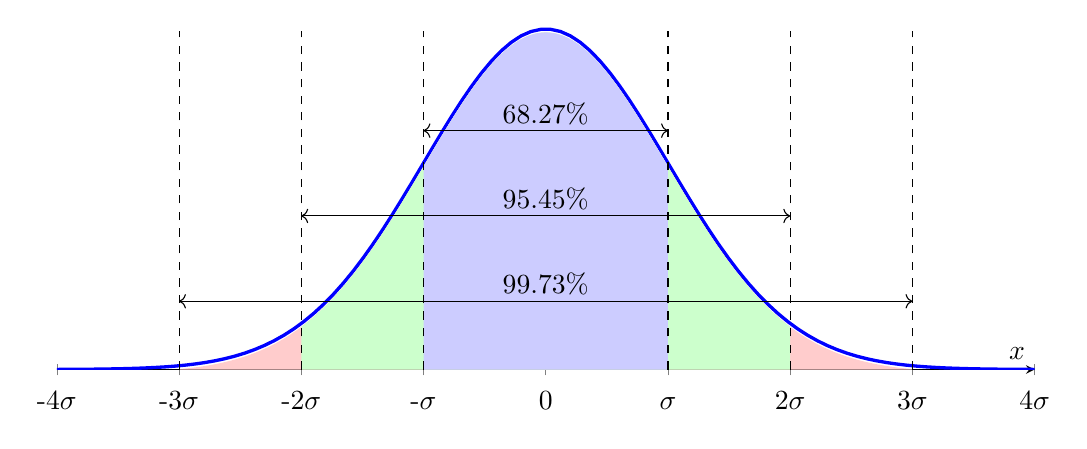
\begin{tikzpicture}
        \begin{axis}[
            no markers, domain=-4:4, samples=100,
            axis lines=center,
            xlabel={$x$},
            axis y line=none,
            ymin=0, ymax=0.5,
            xmin=-4, xmax=4,
            height=7cm, width=14cm,
            ytick=\empty,
            xtick={-4, -3,-2,-1,0,1,2,3, 4},
            xticklabels={-4$\sigma$,-3$\sigma$,-2$\sigma$,-$\sigma$,0,$\sigma$,2$\sigma$,3$\sigma$,4$\sigma$},
            xticklabel style={
            	text height=2ex,
            	text depth=0.25ex
            },
          ]
          % PDF curve
          \addplot [very thick, blue] {1/sqrt(2*pi)*exp(-x^2/2)};
          % Shaded right-tail for z>1.5


          \addplot [draw=none, fill=red!20, domain=-3:3] {1/sqrt(2*pi)*exp(-x^2/2)-0.004} \closedcycle;
          % Vertical guide line
          \draw[dashed] (axis cs:-3,0) -- (axis cs:-3,{1/sqrt(2*pi)*exp(-0.1^2/2)});
          \draw[dashed] (axis cs:3,0) -- (axis cs:3,{1/sqrt(2*pi)*exp(-0.1^2/2)});


          \addplot [draw=none, fill=green!20, domain=-2:2] {1/sqrt(2*pi)*exp(-x^2/2)-0.004} \closedcycle;
          % Vertical guide line
          \draw[dashed] (axis cs:-2,0) -- (axis cs:-2,{1/sqrt(2*pi)*exp(-0.1^2/2)});
          \draw[dashed] (axis cs:2,0) -- (axis cs:2,{1/sqrt(2*pi)*exp(-0.1^2/2)});

          \addplot [draw=none, fill=blue!20, domain=-1:1] {1/sqrt(2*pi)*exp(-x^2/2)-0.004} \closedcycle;
          % Vertical guide line
          \draw[dashed] (axis cs:-1,0) -- (axis cs:-1,{1/sqrt(2*pi)*exp(-0.1^2/2)});
          \draw[dashed] (axis cs:1,0) -- (axis cs:1,{1/sqrt(2*pi)*exp(-0.1^2/2)});

          \node at (axis cs:0,0.3) { $68.27\%$};
          \node at (axis cs:0,0.2) { $95.45\%$};
          \node at (axis cs:0,0.1) { $99.73\%$};

          \draw[<->, black] (axis cs:-3,0.08) -- (axis cs:3,0.08);
          \draw[<->, black] (axis cs:-2,0.18) -- (axis cs:2,0.18);
          \draw[<->, black] (axis cs:-1,0.28) -- (axis cs:1,0.28);
        \end{axis}
      \end{tikzpicture}
  \end{center}

	\item The linear combination of two independent normal variables is also normal.

	\begin{textbox}
		\textbf{Theorem}: Let \( X \sim N(\mu_1, \sigma_1^2) \) and \( Y \sim N(\mu_2, \sigma_2^2) \) be two independent normal random variables. Then for any real constants \( a \) and \( b \), the linear combination
		\[
		Z = aX + bY
		\]
		is also normally distributed with
		\[
		Z \sim N\left( a\mu_1 + b\mu_2,\; a^2 \sigma_1^2 + b^2 \sigma_2^2 \right)
		\]
	\end{textbox}

	\textbf{Proof}: Since \( X \sim N(\mu_1, \sigma_1^2) \), its moment generating function (MGF) is
		\[
		M_X(t) = \exp\left( \mu_1 t + \frac{1}{2} \sigma_1^2 t^2 \right)
		\]
		Similarly, the MGF of \( Y \sim N(\mu_2, \sigma_2^2) \) is
		\[
		M_Y(t) = \exp\left( \mu_2 t + \frac{1}{2} \sigma_2^2 t^2 \right)
		\]

		Consider \( Z = aX + bY \). Since \( X \) and \( Y \) are independent, the MGF of \( Z \) is:
		\[
		M_Z(t) = \mathbb{E}\left( e^{t(aX + bY)}\right)  = \mathbb{E}\left( e^{taX}\right)  \cdot \mathbb{E}\left( e^{tbY}\right)  = M_X(at) \cdot M_Y(bt)
		\]

		Substituting the MGFs:
		\[
		M_Z(t) = \exp\left( a\mu_1 t + \frac{1}{2} a^2 \sigma_1^2 t^2 \right) \cdot \exp\left( b\mu_2 t + \frac{1}{2} b^2 \sigma_2^2 t^2 \right)
		\]

		Combining the exponents:
		\[
		M_Z(t) = \exp\left( (a\mu_1 + b\mu_2)t + \frac{1}{2}(a^2 \sigma_1^2 + b^2 \sigma_2^2)t^2 \right)
		\]

		This is the MGF of a normal distribution with mean \( a\mu_1 + b\mu_2 \) and variance \( a^2 \sigma_1^2 + b^2 \sigma_2^2 \). Therefore,
		\[
		Z \sim N\left( a\mu_1 + b\mu_2,\; a^2 \sigma_1^2 + b^2 \sigma_2^2 \right)
		\]

		\hfill $\blacksquare$


\end{enumerate}



\subsection{Standard Normal Distribution:}

When $\mu = 0$ and $\sigma^2 = 1$, the normal distribution is called the \textbf{standard normal distribution}, denoted as:
\[
Z \sim \mathcal{N}(0, 1)
\]

Its PDF becomes:
\begin{textbox}
\[
f_Z(z) = \frac{1}{\sqrt{2\pi}} \exp\left( -\frac{z^2}{2} \right)
\]
\end{textbox}


Cumulative PDF:
\begin{textbox}
$$F_Z(z) = P(Z \leq z) = \int_{-\infty}^z f_Z(t)dt$$
\end{textbox}

\vspace{2mm}

\begin{center}
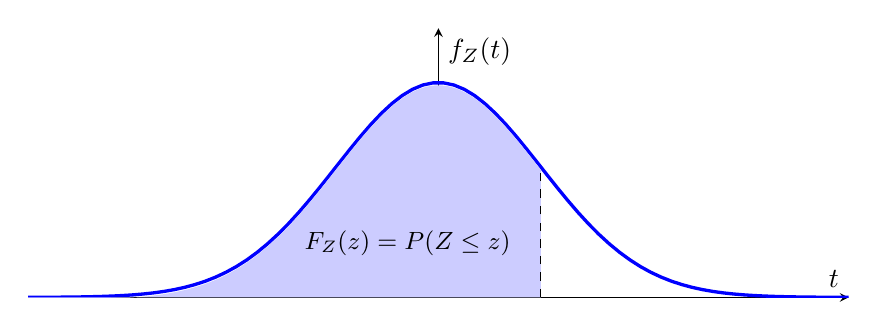
\begin{tikzpicture}
      \begin{axis}[
          no markers, domain=-5:5, samples=100,
          axis lines=center,
          xlabel={$t$}, ylabel={$f_Z(t)$},
          ymin=0, ymax=0.5,
          xmin=-4, xmax=4,
          height=5cm, width=12cm,
          xtick=\empty, ytick=\empty
        ]
        % PDF curve
        \addplot [very thick, blue] {1/sqrt(2*pi)*exp(-x^2/2)};
        % Shaded right-tail for z>1.5
        \addplot [draw=none, fill=blue!20, domain=-4:1] {1/sqrt(2*pi)*exp(-x^2/2)-0.005} \closedcycle;
        % Vertical guide line
        \draw[dashed] (axis cs:1,0) -- (axis cs:1,{1/sqrt(2*pi)*exp(-1^2/2)});
        \node at (axis cs:-0.3,0.1) {\small $F_Z(z) = P(Z\leq z)$};
      \end{axis}
    \end{tikzpicture}
\end{center}

\begin{textbox}
\textbf{Theorem.} Let \( X \sim N(\mu, \sigma^2) \) be a normally distributed random variable and let \( Z \sim N(0, 1) \) be a standard normal random variable. Then, for any real number \( k \),
\[
F_X(k) = F_Z\left( \frac{k - \mu}{\sigma} \right)
\]
where \( F_X \) and \( F_Z \) denote the cumulative distribution functions of \( X \) and \( Z \), respectively.
\end{textbox}

\textbf{Proof}: Define the function
\[
z = g(x) \;=\; \frac{x - \mu}{\sigma},
\]
which is strictly increasing (since \(\sigma>0\)) and differentiable, with inverse
\[
g^{-1}(y) = x \;=\; \sigma z + \mu
\]
Set
\[
Y \;=\; g(X) \;=\; \frac{X - \mu}{\sigma}
\]
Then \(Y\) has the same distribution as \(Z\), i.e.\ \(Y\sim N(0,1)\).  By the change‐of‐variable theorem for CDFs (strictly increasing case),
\[
F_Z(z)
\;=\;
P\bigl(Z \le z\bigr)
\;=\;
F_X\!\bigl(g^{-1}(z)\bigr)
\]
Hence,
\[
F_Z(z)
\;=\;
F_X\!\bigl(\sigma z + \mu\bigr)
\]
Now replace \(z\) by \(\tfrac{k-\mu}{\sigma}\).  Since
\(\sigma\cdot\tfrac{k-\mu}{\sigma} + \mu = k\), we obtain
\[
F_Z\!\left( \dfrac{k - \mu}{\sigma}\right)  = F_X(k)
\]
as required.


\hfill $\blacksquare$

Any normal random variable $X \sim \mathcal{N}(\mu, \sigma^2)$ can be converted to a \textbf{standard normal variable} using the transformation:
\[
Z = \dfrac{X - \mu}{\sigma}
\]

\begin{textbox}
\textbf{Theorem}: Let \( Z \sim N(0,1) \) be a standard normal random variable with CDF \( F_Z(z) \). Then, for any real number \( k \),
\[
F_Z(-k) = 1 - F_Z(k)
\]
\end{textbox}

Since $f_Z(z)$ is symmetrical about zero, so for any $k$
$$f_Z(-k) = f_Z(k)$$
Now,
\begin{align*}
F_Z(-k)
&= P(Z \le -k) \\
&= \int_{-\infty}^{-k} f_Z(z)dz\\
\intertext{Change variable $t=-z$, so when $z=-\infty\to t=+\infty$, and $z=-k\to t=k$, with $dz=-dt$:}
F_Z(-k) &= \int_{\infty}^{k} f_Z(-t)\,(-dt) \\
&= -\int_{\infty}^{k} f_Z(t)\,dt \\
&= \int_{k}^{\infty} f_Z(t)dt\\
&= P(Z \ge k)\\
&= 1 - P(Z < k)\\
&= 1 - F_Z(k)
\end{align*}

\hfill $\blacksquare$

\subsection{Standard Normal Table}

The \textbf{standard normal table} (or $Z$-table)  shown in Table~\ref{table:Ztable} is used to quickly find cumulative probabilities for the standard normal distribution \(Z\sim\mathcal{N}(0,1)\) without evaluating the integral $$\int_{-\infty}^z \frac{1}{\sqrt{2\pi}}e^{-t^2/2}\,dt$$ by hand.  By converting any normal random variable \(X\sim N(\mu,\sigma^2)\) into the standard form \(Z=(X-\mu)/\sigma\), one can look up probabilities such as \(P(X\le x)\) in a single, universal table, greatly simplifying calculations in statistical inference and hypothesis testing.


\begin{table}[!h]
\centering
\footnotesize
\caption{\small Standard Normal CDF values $F_Z(z)=P(Z\le z)$}
\label{table:Ztable}
\begin{tabular}{l|*{10}{r}}
\toprule
z   & 0       & 0.01    & 0.02    & 0.03    & 0.04    & 0.05    & 0.06    & 0.07    & 0.08    & 0.09    \\
\midrule
0   & 0.5     & 0.50399 & 0.50798 & 0.51197 & 0.51595 & 0.51994 & 0.52392 & 0.5279  & 0.53188 & 0.53586 \\
0.1 & 0.53983 & 0.5438  & 0.54776 & 0.55172 & 0.55567 & 0.55962 & 0.56356 & 0.56749 & 0.57142 & 0.57535 \\
0.2 & 0.57926 & 0.58317 & 0.58706 & 0.59095 & 0.59483 & 0.59871 & 0.60257 & 0.60642 & 0.61026 & 0.61409 \\
0.3 & 0.61791 & 0.62172 & 0.62552 & 0.6293  & 0.63307 & 0.63683 & 0.64058 & 0.64431 & 0.64803 & 0.65173 \\
0.4 & 0.65542 & 0.6591  & 0.66276 & 0.6664  & 0.67003 & 0.67364 & 0.67724 & 0.68082 & 0.68439 & 0.68793 \\
0.5 & 0.69146 & 0.69497 & 0.69847 & 0.70194 & 0.7054  & 0.70884 & 0.71226 & 0.71566 & 0.71904 & 0.7224  \\
0.6 & 0.72575 & 0.72907 & 0.73237 & 0.73565 & 0.73891 & 0.74215 & 0.74537 & 0.74857 & 0.75175 & 0.7549  \\
0.7 & 0.75804 & 0.76115 & 0.76424 & 0.7673  & 0.77035 & 0.77337 & 0.77637 & 0.77935 & 0.7823  & 0.78524 \\
0.8 & 0.78814 & 0.79103 & 0.79389 & 0.79673 & 0.79955 & 0.80234 & 0.80511 & 0.80785 & 0.81057 & 0.81327 \\
0.9 & 0.81594 & 0.81859 & 0.82121 & 0.82381 & 0.82639 & 0.82894 & 0.83147 & 0.83398 & 0.83646 & 0.83891 \\
1   & 0.84134 & 0.84375 & 0.84614 & 0.84849 & 0.85083 & 0.85314 & 0.85543 & 0.85769 & 0.85993 & 0.86214 \\
1.1 & 0.86433 & 0.8665  & 0.86864 & 0.87076 & 0.87286 & 0.87493 & 0.87698 & 0.879   & 0.881   & 0.88298 \\
1.2 & 0.88493 & 0.88686 & 0.88877 & 0.89065 & 0.89251 & 0.89435 & 0.89617 & 0.89796 & 0.89973 & 0.90147 \\
1.3 & 0.9032  & 0.9049  & 0.90658 & 0.90824 & 0.90988 & 0.91149 & 0.91309 & 0.91466 & 0.91621 & 0.91774 \\
1.4 & 0.91924 & 0.92073 & 0.9222  & 0.92364 & 0.92507 & 0.92647 & 0.92785 & 0.92922 & 0.93056 & 0.93189 \\
1.5 & 0.93319 & 0.93448 & 0.93574 & 0.93699 & 0.93822 & 0.93943 & 0.94062 & 0.94179 & 0.94295 & 0.94408 \\
1.6 & 0.9452  & 0.9463  & 0.94738 & 0.94845 & 0.9495  & 0.95053 & 0.95154 & 0.95254 & 0.95352 & 0.95449 \\
1.7 & 0.95543 & 0.95637 & 0.95728 & 0.95818 & 0.95907 & 0.95994 & 0.9608  & 0.96164 & 0.96246 & 0.96327 \\
1.8 & 0.96407 & 0.96485 & 0.96562 & 0.96638 & 0.96712 & 0.96784 & 0.96856 & 0.96926 & 0.96995 & 0.97062 \\
1.9 & 0.97128 & 0.97193 & 0.97257 & 0.9732  & 0.97381 & 0.97441 & 0.975   & 0.97558 & 0.97615 & 0.9767  \\
2   & 0.97725 & 0.97778 & 0.97831 & 0.97882 & 0.97932 & 0.97982 & 0.9803  & 0.98077 & 0.98124 & 0.98169 \\
2.1 & 0.98214 & 0.98257 & 0.983   & 0.98341 & 0.98382 & 0.98422 & 0.98461 & 0.985   & 0.98537 & 0.98574 \\
2.2 & 0.9861  & 0.98645 & 0.98679 & 0.98713 & 0.98745 & 0.98778 & 0.98809 & 0.9884  & 0.9887  & 0.98899 \\
2.3 & 0.98928 & 0.98956 & 0.98983 & 0.9901  & 0.99036 & 0.99061 & 0.99086 & 0.99111 & 0.99134 & 0.99158 \\
2.4 & 0.9918  & 0.99202 & 0.99224 & 0.99245 & 0.99266 & 0.99286 & 0.99305 & 0.99324 & 0.99343 & 0.99361 \\
2.5 & 0.99379 & 0.99396 & 0.99413 & 0.9943  & 0.99446 & 0.99461 & 0.99477 & 0.99492 & 0.99506 & 0.9952  \\
2.6 & 0.99534 & 0.99547 & 0.9956  & 0.99573 & 0.99585 & 0.99598 & 0.99609 & 0.99621 & 0.99632 & 0.99643 \\
2.7 & 0.99653 & 0.99664 & 0.99674 & 0.99683 & 0.99693 & 0.99702 & 0.99711 & 0.9972  & 0.99728 & 0.99736 \\
2.8 & 0.99744 & 0.99752 & 0.9976  & 0.99767 & 0.99774 & 0.99781 & 0.99788 & 0.99795 & 0.99801 & 0.99807 \\
2.9 & 0.99813 & 0.99819 & 0.99825 & 0.99831 & 0.99836 & 0.99841 & 0.99846 & 0.99851 & 0.99856 & 0.99861 \\
3   & 0.99865 & 0.99869 & 0.99874 & 0.99878 & 0.99882 & 0.99886 & 0.99889 & 0.99893 & 0.99896 & 0.999   \\
3.1 & 0.99903 & 0.99906 & 0.9991  & 0.99913 & 0.99916 & 0.99918 & 0.99921 & 0.99924 & 0.99926 & 0.99929 \\
3.2 & 0.99931 & 0.99934 & 0.99936 & 0.99938 & 0.9994  & 0.99942 & 0.99944 & 0.99946 & 0.99948 & 0.9995  \\
3.3 & 0.99952 & 0.99953 & 0.99955 & 0.99957 & 0.99958 & 0.9996  & 0.99961 & 0.99962 & 0.99964 & 0.99965 \\
3.4 & 0.99966 & 0.99968 & 0.99969 & 0.9997  & 0.99971 & 0.99972 & 0.99973 & 0.99974 & 0.99975 & 0.99976 \\
3.5 & 0.99977 & 0.99978 & 0.99978 & 0.99979 & 0.9998  & 0.99981 & 0.99981 & 0.99982 & 0.99983 & 0.99983 \\
3.6 & 0.99984 & 0.99985 & 0.99985 & 0.99986 & 0.99986 & 0.99987 & 0.99987 & 0.99988 & 0.99988 & 0.99989 \\
3.7 & 0.99989 & 0.9999  & 0.9999  & 0.9999  & 0.99991 & 0.99991 & 0.99992 & 0.99992 & 0.99992 & 0.99992 \\
3.8 & 0.99993 & 0.99993 & 0.99993 & 0.99994 & 0.99994 & 0.99994 & 0.99994 & 0.99995 & 0.99995 & 0.99995 \\
3.9 & 0.99995 & 0.99995 & 0.99996 & 0.99996 & 0.99996 & 0.99996 & 0.99996 & 0.99996 & 0.99997 & 0.99997 \\
4   & 0.99997 & 0.99997 & 0.99997 & 0.99997 & 0.99997 & 0.99997 & 0.99998 & 0.99998 & 0.99998 & 0.99998 \\
\addlinespace
\bottomrule
\end{tabular}
\end{table}

To look up \(F_Z(k)\), follow the following steps:

\begin{enumerate}
  \item Write \(k\) to \textbf{two decimal places}, e.g.\ \(k=1.23\).
  \item Split into
    \[
      \text{row part} = 1.2,\quad
      \text{column part} = 0.03
    \]
  \item In Table~\ref{table:Ztable}, go to the row labeled “1.2” and the column
    labeled “0.03”.  The entry at their intersection is
    \[
      F_Z(1.23) = P(Z\le 1.23) \;=\; 0.89065
    \]
  \item For negative \(z\), use symmetry:
    \[
      F_Z(-k) = P(Z\le -k)
      = 1 - P(Z\le k) = 1 - F_Z(k)
    \]
  \item For right‐tail probabilities,
    \[
      P(Z>k) = 1 - F_Z(k)
    \]
  \item For probabilities within a specified interval of $ Z $ values,
  $$P(k_1 \leq Z \leq k_2) = P(Z \leq k_2) - P(Z \leq k_1) = F_Z(k_2) - F_Z(k_1)$$
\end{enumerate}

\textbf{Example:} Suppose the heights of adult males are normally distributed with mean $\mu = 175$ cm and standard deviation $\sigma = 10$ cm. Let $X$ denote the height of a randomly chosen male. Then:
\[
X \sim \mathcal{N}(175, 100)
\]

What is the probability that a randomly chosen male is taller than 190 cm?

We standardize:
\[
Z = \frac{190 - 175}{10} = 1.5
\]

Using the standard normal table:
\[
P(X > 190) = P(Z > 1.5) = 1 - F_Z(1.5) \approx 1 - 0.9332 = 0.0668
\]

Thus, approximately $6.68\%$ of adult males are taller than 190 cm.


% \begin{table}[!h]
%   \centering
%   \footnotesize
%   \caption{Standard Normal CDF values $F_Z(z)=P(Z\le z)$.}
%   \label{tab:Ztable}
%   \begin{tabular}{l|*{10}{r}}
%     \toprule
%     $z$ & 0    & 0.01  & 0.02  & 0.03  & 0.04  & 0.05  & 0.06  & 0.07  & 0.08  & 0.09  \\
%     \midrule
%     0.0 & 0.5000 & 0.50399 & 0.50798 & 0.51197 & 0.51595 & 0.51994 & 0.52392 & 0.52790 & 0.53188 & 0.53586 \\
%     0.1 & 0.53983 & 0.54380 & 0.54776 & 0.55172 & 0.55567 & 0.55962 & 0.56356 & 0.56749 & 0.57142 & 0.57535 \\
%     0.2 & 0.57926 & 0.58317 & 0.58706 & 0.59095 & 0.59483 & 0.59871 & 0.60257 & 0.60642 & 0.61026 & 0.61409 \\
%     0.3 & 0.61791 & 0.62172 & 0.62552 & 0.62930 & 0.63307 & 0.63683 & 0.64058 & 0.64431 & 0.64803 & 0.65173 \\
%     0.4 & 0.65542 & 0.65910 & 0.66276 & 0.66640 & 0.67003 & 0.67364 & 0.67724 & 0.68082 & 0.68439 & 0.68793 \\
%     0.5 & 0.69146 & 0.69497 & 0.69847 & 0.70194 & 0.70540 & 0.70884 & 0.71226 & 0.71566 & 0.71904 & 0.72240 \\
%     0.6 & 0.72575 & 0.72907 & 0.73237 & 0.73565 & 0.73891 & 0.74215 & 0.74537 & 0.74857 & 0.75175 & 0.75490 \\
%     0.7 & 0.75804 & 0.76115 & 0.76424 & 0.76730 & 0.77035 & 0.77337 & 0.77637 & 0.77935 & 0.78230 & 0.78524 \\
%     0.8 & 0.78814 & 0.79103 & 0.79389 & 0.79673 & 0.79955 & 0.80234 & 0.80511 & 0.80785 & 0.81057 & 0.81327 \\
%     0.9 & 0.81594 & 0.81859 & 0.82121 & 0.82381 & 0.82639 & 0.82894 & 0.83147 & 0.83398 & 0.83646 & 0.83891 \\
%     1.0 & 0.84134 & 0.84375 & 0.84614 & 0.84849 & 0.85083 & 0.85314 & 0.85543 & 0.85769 & 0.85993 & 0.86214 \\
%     1.1 & 0.86433 & 0.86650 & 0.86864 & 0.87076 & 0.87286 & 0.87493 & 0.87698 & 0.87900 & 0.88100 & 0.88298 \\
%     1.2 & 0.88493 & 0.88686 & 0.88877 & 0.89065 & 0.89251 & 0.89435 & 0.89617 & 0.89796 & 0.89973 & 0.90147 \\
%     1.3 & 0.90320 & 0.90490 & 0.90658 & 0.90824 & 0.90988 & 0.91149 & 0.91309 & 0.91466 & 0.91621 & 0.91774 \\
%     1.4 & 0.91924 & 0.92073 & 0.92220 & 0.92364 & 0.92507 & 0.92647 & 0.92785 & 0.92922 & 0.93056 & 0.93189 \\
%     1.5 & 0.93319 & 0.93448 & 0.93574 & 0.93699 & 0.93822 & 0.93943 & 0.94062 & 0.94179 & 0.94295 & 0.94408 \\
%     \addlinespace
%     \bottomrule
%   \end{tabular}
% \end{table}

\begin{figure}[!h]
  \centering
  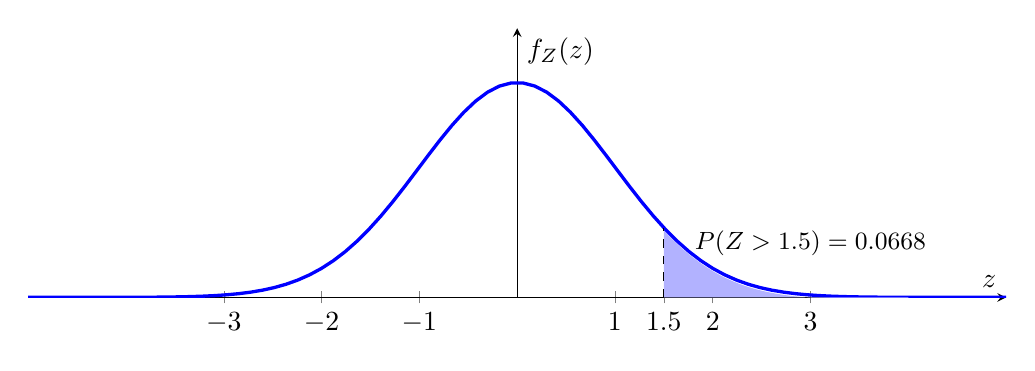
\begin{tikzpicture}
    \begin{axis}[
        no markers, domain=-6:6, samples=100,
        axis lines=center,
        xlabel={$z$}, ylabel={$f_Z(z)$},
        ymin=0, ymax=0.5,
        xmin=-5, xmax=5,
        height=5cm, width=14cm,
        xtick={-3,-2,-1,0,1,1.5,2,3},
        ytick=\empty
      ]
      % PDF curve
      \addplot [very thick, blue] {1/sqrt(2*pi)*exp(-x^2/2)};
      % Shaded right-tail for z>1.5
      \addplot [draw=none, fill=blue!30, domain=1.5:4] {1/sqrt(2*pi)*exp(-x^2/2)-0.005} \closedcycle;
      % Vertical guide line
      \draw[dashed] (axis cs:1.5,0) -- (axis cs:1.5,{1/sqrt(2*pi)*exp(-1.5^2/2)});
      \node at (axis cs:3,0.1) {\small $P(Z>1.5)=0.0668$};
    \end{axis}
  \end{tikzpicture}
\end{figure}

\subsection{Critical Points of the Standard Normal Distribution}

In the standard normal distribution, certain values on the horizontal axis divide the distribution into regions with specified probabilities. These special values are called \textbf{critical points}.

\textbf{One‐sided critical point}: For a given probability \(\alpha\), the one‐sided critical point $z_{\alpha}$ is such that
\[
P(Z > z_{\alpha}) = \alpha
\]
or equivalently \(P(Z \le z_{\alpha}) = 1 - \alpha\).

\begin{center}
	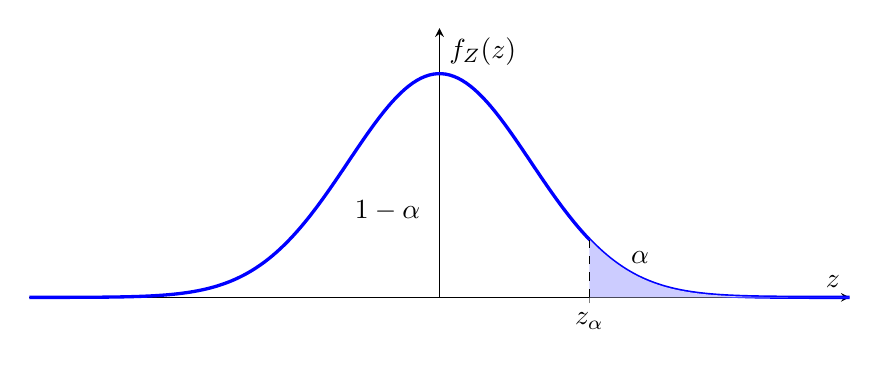
\begin{tikzpicture}
	\begin{axis}[
	no markers, domain=-4.5:4.5, samples=200,
	axis lines=center, %axis y line=none,
	xlabel={$z$}, ylabel={$f_Z(z)$},
	ymin=0, ymax=0.48, xmin=-4.5, xmax=4.5,
	height=5cm, width=12cm,
	xtick={0, 1.645}, xticklabels={0, \(z_{\alpha}\)},
	ytick=\empty, clip=false
	]
	% PDF curve
	\addplot [very thick, blue] {1/sqrt(2*pi)*exp(-x^2/2)};
	% Shade right tail
	\addplot [domain=1.645:4.5, draw=none, fill=blue!20] {1/sqrt(2*pi)*exp(-x^2/2)} \closedcycle;
	% Dashed line
	\draw[dashed] (axis cs:1.645,0) -- (axis cs:1.645,{1/sqrt(2*pi)*exp(-1.645^2/2)});
	% Labels
	\node[below] at (axis cs:2.2,0.1) {\(\alpha\)};
	\node[above] at (axis cs:-0.57,0.12) {\(1 - \alpha\)};
	\end{axis}
	\end{tikzpicture}
\end{center}

\begin{itemize}
	\item For \(\alpha = 0.05\), the one‐sided critical point is approximately \(z_{0.05} \approx 1.645\).
	\item For \(\alpha = 0.01\), the one‐sided critical point is approximately \(z_{0.01} \approx 2.326\).
\end{itemize}

\textbf{Two‐sided critical points}: For a given probability \(\alpha\), the two‐sided critical points \(\pm z_{\alpha/2}\) are such that

\[
P(Z > z_{\alpha/2}) = \alpha/2, \quad P(Z < -z_{\alpha/2}) = \alpha/2
\]
or equivalently
\[
P(-z_{\alpha/2} \le Z \le z_{\alpha/2}) \;=\; 1 - \alpha
\]

\begin{center}
	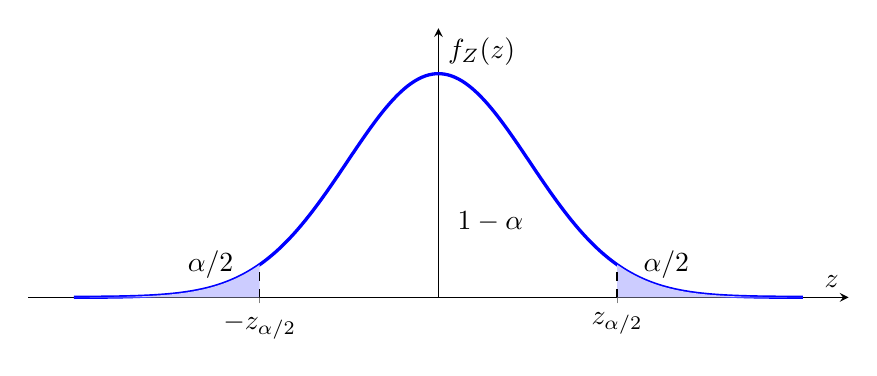
\begin{tikzpicture}
	\begin{axis}[
	no markers, domain=-4:4, samples=200,
	axis lines=center,
	%axis y line=none,
	xlabel={$z$}, ylabel={$f_Z(z)$},
	ymin=0, ymax=0.48,
	xmin=-4.5, xmax=4.5,
	height=5cm, width=12cm,
	xtick={-1.96,0,1.96},
	xticklabels={\(-z_{\alpha/2}\), 0, \(z_{\alpha/2}\)},
	ytick=\empty,
	clip=false
	]
	% PDF curve of standard normal
	\addplot [very thick, blue] {1/sqrt(2*pi)*exp(-x^2/2)};

	% Shade the confidence interval region [-z_alpha/2, z_alpha/2]
	\addplot [
	domain=-4:-1.96,
	draw=none,
	fill=blue!20,
	samples=100
	]
	{1/sqrt(2*pi)*exp(-x^2/2)} \closedcycle;

	\addplot [
	domain=1.96:4,
	draw=none,
	fill=blue!20,
	samples=100
	]
	{1/sqrt(2*pi)*exp(-x^2/2)} \closedcycle;

	% Vertical dashed lines at -z_alpha/2 and z_alpha/2
	\draw[dashed] (axis cs:-1.96,0) -- (axis cs:-1.96,{1/sqrt(2*pi)*exp(-1.96^2/2)});
	\draw[dashed] (axis cs:1.96,0) -- (axis cs:1.96,{1/sqrt(2*pi)*exp(-1.96^2/2)});

	% Labels
	\node[below] at (axis cs:-2.5,0.1) { ${\alpha/2}$};
	\node[below] at (axis cs:2.5,0.1) { ${\alpha/2}$};
	\node[above, black] at (axis cs:0.57,0.1) { \(1-\alpha\)};
	\end{axis}
	\end{tikzpicture}
\end{center}

\begin{itemize}
	\item For \(\alpha = 0.05\), the two-sided critical points are approximately \(\pm 1.96\).
	\item For \(\alpha = 0.01\), the two-sided critical points are approximately \(\pm 2.576\).
\end{itemize}

These critical points help us identify how extreme a value is relative to the overall distribution, and they are fundamental when constructing intervals to estimate population parameters. These critical points are used in hypothesis tests and to construct confidence intervals which we will see in future chapters.

\chapter{Sampling Theory}
\section{Introduction}
Sampling theory is a part of statistics that helps us understand how to learn about a large group by looking at just a small part of it. For example, imagine a company makes a new type of battery and wants to know how long the batteries last. Testing every single battery would take too much time and money, so the company picks a few batteries to test. These few batteries are called a \textbf{sample}, and all the batteries made by the company are called the \textbf{population}.

The company really wants to know the average lifetime of all batteries—this is called a \textbf{parameter}. But since they can’t test them all, they use the average lifetime from the sample—this is called a \textbf{statistic}.

Sampling theory helps us understand how close this statistic is likely to be to the real average. It also helps us decide how many batteries to test and how to choose them so we get useful, reliable results.

\begin{textbox}
    \textbf{Population}: The entire group of individuals or items that we want to learn about.
    Example: All the batteries produced by a company.

    \vspace{3mm}
    \textbf{Sample}: A smaller group taken from the population, which is actually tested or studied.
    Example: 100 batteries chosen from the whole production batch.

    \vspace{3mm}
    \textbf{Parameter}: A numerical value that describes a characteristic of the population (usually unknown).
    Example: The true average lifetime of all the batteries.

    \vspace{3mm}
    \textbf{Statistic}: A numerical value that describes a characteristic of the sample (used to estimate the parameter).
    Example: The average lifetime of the 100 batteries tested.
\end{textbox}

\section{Sampling Methods}

\subsection{Simple Random Sampling}

\begin{textbox}
A \textbf{simple random sampling} is one in which every member of the population has an equal chance of being selected in the sample.
\end{textbox}
 Mathematically, this means that each possible sample of size $n$ from a population has the same probability of being chosen. For example, suppose a factory produces 10,000 batteries in a day. To estimate the average lifespan, 100 batteries are selected randomly so that each battery has the same chance of inclusion. An important advantage of simple random sampling is that it is straightforward to analyze using statistical theory, which makes inference about the population simpler

In this text, we will limit our discussion to \textbf{simple random sampling}.  Before a random sample of size $n$ is selected, the observations are modeled as the random variables $X_1 , X_2, \dots , X_n$. For example, if we randomly select 5 light bulbs from a production batch, their lifespans can be represented by the random variables \( X_1, X_2, X_3, X_4, X_5 \), each denoting the lifespan (in hours) of a selected bulb.

\begin{align*}
    X_1 &= \text{Lifespan (in hours) of 1st selected bulb} \\
    X_2 &= \text{Lifespan (in hours) of 2nd selected bulb} \\
    &\dots \\
    X_5 &= \text{Lifespan (in hours) of 5th selected bulb}
\end{align*}


Assume a first draw yields the following lifespans (in hours) for \(n = 5\) randomly selected light bulbs:
\[
\text{Draw 1:} \quad \{X_1=1200, X_2=1140, X_3=1180, X_4=1300, X_5=1250\}
\]

Because each sample is chosen at random, a fresh draw of five bulbs would almost surely yield different numerical values for \(X_1, X_2, \dots, X_5\). Assume a second draw produces:
\[
\text{Draw 2:} \quad \{X_1=1400, X_2=1550, X_3=1200, X_4=1420, X_5=1380\}
\]

In this way, each \(X_i\) behaves as a genuine random variable, capturing the uncertainty inherent in the sampling process.

There are two main types of simple random sampling:

\begin{enumerate}
    \item \textbf{Simple Random Sampling With Replacement (SRSWR)}: This is a method of selecting a sample of size \( n \) from a population of size \( N \) one by one such that after each stage of selection, the element is returned to the population before the next draw. Because each selection is made from the full population, the sample observations \( X_1, X_2, \dots, X_n \) are \textit{independent and identically distributed (i.i.d.)}\footnote{%
    \textbf{Independent and Identically Distributed (i.i.d.)} is a fundamental assumption in statistics. \textit{Identically distributed} means that each random variable \( X_i \) follows the same probability distribution (e.g., normal, binomial). \textit{Independent} means the outcome of one observation does not influence or provide information about the others; knowing \( X_1 \) gives no information about \( X_2, X_3, \) etc.
} random variables following the population distribution.

    \item \textbf{Simple Random Sampling Without Replacement (SRSWOR)}: This is a method of selecting a sample of size \( n \) from a population of size \( N \) one by one such that after each stage of selection, the element is not returned to the population. So there is no chance of a particular item being selected twice in the sample. Although the sample observations \( X_1, X_2, \dots, X_n \) are identically distributed (each has the same marginal distribution), they are \textit{not independent}, due to the changing composition of the population after each draw.
\end{enumerate}


\subsection{Other Sampling Methods}

\begin{enumerate}
    \item \textbf{Stratified Sampling}: In stratified sampling, the population is divided into distinct subgroups or strata based on a specific characteristic (e.g., age, income, region), and a random sample is drawn from each stratum. This method ensures representation from all key subgroups.

\textit{Example:} A company wants to sample employee opinions. Employees are divided into departments (e.g., HR, Sales, R\&D), and a random sample is taken from each department.

\textit{Advantages:} Increases accuracy by reducing variability; ensures important groups are represented.

\textit{Disadvantages:} Requires knowledge of strata and population characteristics in advance.

\item \textbf{Systematic Sampling}: Systematic sampling selects every $k$-th individual from a population list after a random starting point. The interval $k$ is calculated by dividing the population size by the desired sample size.

\textit{Example:} If a company has a list of 1,000 employees and wants to survey 100, it selects a random starting point between 1 and 10, then picks every 10th employee on the list.

\textit{Advantages:} Simple and quick to implement; useful when population is ordered.

\textit{Disadvantages:} Can introduce bias if there is a hidden pattern in the population that coincides with the sampling interval.

\item \textbf{Cluster Sampling}: In cluster sampling, the population is divided into clusters (often based on geography or natural groupings). A few clusters are randomly selected, and then all individuals within those clusters are included in the sample.

\textit{Example:} A research team wants to survey households in a city. The city is divided into neighborhoods (clusters), a few neighborhoods are selected at random, and all households in those neighborhoods are surveyed.

\textit{Advantages:} Cost-effective and practical for large, dispersed populations.

\textit{Disadvantages:} Can lead to higher sampling error if clusters are not homogeneous.

\item \textbf{Multistage Sampling}: Multistage sampling combines several sampling techniques. Typically, it begins with cluster sampling to select large groups, and then simple random or stratified sampling is used within those groups.

\textit{Example:} In a national education survey, schools are randomly selected (cluster sampling), then students within each selected school are randomly chosen (simple random sampling).

\textit{Advantages:} Flexible and practical for large-scale surveys; reduces cost and time.

\textit{Disadvantages:} More complex design and analysis; potential for increased sampling error if stages are not carefully planned.
\end{enumerate}

\section{Sample Mean, Sample Variance and Sample Proportion}

Let \( X_1, X_2, \dots, X_n \) be a random sample of size \( n \) drawn from a population which are modeled as random variables. The \textbf{sample mean} is defined as:
\begin{textbox}
     \[
\text{Sample Mean} = \overline{X} = \frac{1}{n} \sum_{i=1}^{n} X_i
\]
\end{textbox}
It represents the average of the observed sample values.

The \textbf{sample variance} is defined as:
\begin{textbox}
\[
\text{Sample Variance} = S^2 = \frac{1}{n - 1} \sum_{i=1}^{n} (X_i - \overline{X})^2
\]
\end{textbox}
This measures the spread or variability of the sample values around the sample mean. The denominator \( n - 1 \) (instead of \( n \)) ensures that \( S^2 \) is an \emph{unbiased estimator} of the population variance \( \sigma^2 \). We will discussed the concept of unbiased estimator in later chapter.

The \textbf{sample standard deviation} is the positive square root of the sample variance:
\begin{textbox}
\[
\text{Sample Standard Deviation} = S = \sqrt{\frac{1}{n - 1} \sum_{i=1}^{n} (X_i - \overline{X})^2}
\]
\end{textbox}

Now let's suppose \( X_i \) is modeled as a binary indicator variable where

\[
X_i = \begin{cases}
1, & \text{if the } i\text{-th observation has the characteristic of interest} \\
0, & \text{otherwise}
\end{cases}
\]

The \textbf{sample proportion} for the the characteristic of interest is defined as:
\begin{textbox}
\[
\text{Sample Proportion} = \hat{p} = \frac{1}{n} \sum_{i=1}^n X_i = \frac{X}{n}
\]
\end{textbox}

It represents the fraction of the sample exhibiting the characteristic of interest and serves as an estimator of the population proportion \( p \).



\section{Sampling Distributions}
The value of any statistic (e.g. sample mean) will vary from sample to sample.
\begin{textbox}
The \textbf{sampling distribution} of a statistic is the probability distribution of the statistic's values computed from all possible random samples of the same size taken from a given population.
\end{textbox}

Suppose a factory produces thousands of batteries, and the lifetimes of these batteries follow a distribution with a population mean \( \mu = 100 \) hours and a population standard deviation \( \sigma = 20 \) hours.

Now, imagine taking a random sample of 5 batteries and computing the average lifetime (sample mean). You repeat this process many times—each time taking a new random sample of 5 batteries and calculating its mean. Each of these sample means will be a bit different due to natural variation in the samples. If you plot all these sample means on a graph, the result is the \textbf{sampling distribution of the sample mean}.

The standard deviation of the sampling distribution of a statistic is given a specific name — it is called the \textbf{standard error} of that sample statistic.

\begin{textbox}
The \textbf{standard error} of a sample statistic is the standard deviation of its sampling distribution. It measures how much the statistic is expected to vary from sample to sample due to random chance.
\end{textbox}

\section{The Sampling Distribution of the Sample Mean}

\begin{textbox}
\textbf{Theorem}: Let $X_1 , X_2, \dots , X_n$ be random samples of size $n$ \textit{chosen with replacements} from a population with mean $\mu$ and variance $\sigma^2$, then
$$\mathbb{E}(\overline{X}) = \mu,  \text{ and } \mathrm{Var}(\overline{X}) = \dfrac{\sigma^2}{n}$$
\end{textbox}
% This theorem is also true when the population size in infinite.

\textbf{Proof}: We assume the population consists of $N$ elements $\{y_1, y_2, \dots, y_N\}$. The population mean and population variance are defined as:

$$\mu = \dfrac{1}{N}\sum_{j=1}^N y_j, \quad \sigma^2 = \dfrac{1}{N}\sum_{j=1}^N (y_j - \mu)^2$$

The sample mean is defined as:
\[
\overline{X} = \frac{1}{n} \sum_{i=1}^{n} X_i
\]

By the linearity of expectation:
\[
\mathbb{E}(\overline{X}) = \mathbb{E}\left( \frac{1}{n} \sum_{i=1}^{n} X_i \right) = \frac{1}{n} \sum_{i=1}^{n} \mathbb{E}(X_i)
\]

Since each \( X_i \) is drawn from the population $\{y_1, y_2, \dots, y_N\}$ each with probability $\dfrac{1}{N}$. Hence, we have for all $i$:
\[
\mathbb{E}(X_i) = \sum_{j=1}^N y_j \cdot \underbrace{(X_i = y_j)}_{1/N}
 = \dfrac{1}{N}\sum_{j=1}^N y_j  = \mu
\]

So:
\[
\mathbb{E}(\overline{X}) = \frac{1}{n} \cdot n \cdot \mu = \mu
\]

Using the formula for the variance of a sum of independent random variables:
\[
\mathrm{Var}(\overline{X}) = \mathrm{Var} \left( \frac{1}{n} \sum_{i=1}^{n} X_i \right) = \frac{1}{n^2} \sum_{i=1}^{n} \mathrm{Var}(X_i)
\]
Now,
$$\mathrm{Var}(X_i) = \sum_{j=1}^N (y_j - \mu)^2 \cdot \underbrace{P(X_i = y_j)}_{1/N} = \dfrac{1}{N}\sum_{j=1}^N (y_j - \mu)^2 = \sigma^2$$
Therefore,
\[
\mathrm{Var}(\overline{X}) = \frac{1}{n^2} \cdot n \cdot \sigma^2 = \frac{\sigma^2}{n}
\]


% \[
% \therefore \quad \mathbb{E}(\overline{X}) = \mu \quad \text{and} \quad \mathrm{Var}(\overline{X}) = \frac{\sigma^2}{n}
% \]

\hfill $\blacksquare$

\begin{textbox}
\textbf{Theorem}: Let $X_1 , X_2, \dots , X_n$ be random samples of size $n$ \textit{chosen without replacement} from a population of size $N$ with mean $\mu$ and variance $\sigma^2$, then
$$\mathbb{E}(\overline{X}) = \mu,  \text{ and } \mathrm{Var}(\overline{X}) = \dfrac{\sigma^2}{n}\left(\dfrac{N-n}{N-1}\right)$$
\end{textbox}

We skip the proof as it is beyond the scope of this text. The term $$\frac{N-n}{N-1}$$ is often called \textbf{finite population correction factor}, is close to 1 (and can be omitted for most practical purposes) unless the sample constitutes a substantial portion
of the population.

% \textbf{Proof}: By definition of sample mean:
% $$\overline{X} = \frac{1}{n} \sum_{i=1}^n X_i$$
% By the linearity of expectation:
% \[
% \mathbb{E}(\overline{X}) = \mathbb{E}\left( \frac{1}{n} \sum_{i=1}^{n} X_i \right) = \frac{1}{n} \sum_{i=1}^{n} \mathbb{E}(X_i)
% \]
% First we need to find out the value of $\mathbb{E}(X_i)$. To do that, let us fix any population value $y_j$ and define the event
% $$
% H = \{\text{$y_j$ not among }X_1,\dots,X_{i-1}\},
% $$
% and its complement $\overline{H}$.  By the law of total probability,
% \[
% P(X_i=y_j)
% = P(X_i=y_j\mid H)\,P(H)
%   + P(X_i=y_j\mid \overline{H})\,P(\overline{H}).
% \]
% - If $\overline{H}$ occurs, then $y_j$ was already drawn, so $P(X_i=y_j\mid \overline{H})=0$.

% - If $H$ occurs, there are $N-(i-1)$ items left each with probability $\dfrac{1}{N-(i-1)}$ of being selected. So
%   $$P(X_i=y_j\mid H)=\frac{1}{N-(i-1)}.
%   $$

% By symmetry, the probability $y_j$ survives the first $i-1$ draws is
%   \begin{align*}
%       P(H)&=\frac{\text{Num of ways }i-1\text{ items can be selected from }N-1\text{ items which excludes }y_j}{\text{Num of ways }i-1\text{ items can be selected from }N\text{ items}} \\
%   &= \frac{\binom{N-1}{i-1}}{\binom{N}{i-1}}=\frac{N-i+1}{N}
%   \end{align*}
% Putting these together,
% \[
% P(X_i=y_j)
% = \frac{1}{N-(i-1)}\cdot\frac{N-i+1}{N}
% = \frac{1}{N},
% \]
% and thus
% \[
% \mathbb{E}(X_i)
% = \sum_{j=1}^N y_j\,P(X_i=y_j)
% = \frac{1}{N}\sum_{j=1}^N y_j
% = \mu.
% \]
% By linearity, $\mathbb{E}(\overline{X})=\mu$.

% Let us now calculate the variance. Since draws are dependent without replacement, we must account for
% covariances. Recall:
% \begin{align*}
% \mathrm{Var}(\overline{X}) &= \mathrm{Var}\left(\frac{1}{n} \sum_{i=1}^{n} X_i\right) = \frac{1}{n^2} \mathrm{Var}\left(\sum_{i=1}^n X_i\right) \\
% &= \frac{1}{n^2} \Bigl(\sum_{i=1}^n \mathrm{Var}(X_i) + 2\sum_{1 \le i < k \le n} \mathrm{Cov}(X_i, X_k)\Bigr)
% \end{align*}

% - For each $i$, as in the with-replacement case,
% $$
% \mathrm{Var}(X_i) = \sigma^2
% $$

% - For $i \neq k$, the covariance of two distinct draws satisfies (see e.g. properties of simple random sampling)
% $$
% \mathrm{Cov}(X_i, X_k) = -\frac{\sigma^2}{N - 1}.
% $$
% (One way to show this is to use the fact that the sum of all $N$ sample indicators is fixed at $n$, giving negative dependence.)

% Substituting into the variance formula,
% \begin{align*}
% \mathrm{Var}(\overline{X})
% &= \frac{1}{n^2} \Bigl(n\sigma^2 + 2\binom{n}{2} \Bigl(-\frac{\sigma^2}{N - 1}\Bigr)\Bigr) \\[6pt]
% &= \frac{1}{n^2} \Bigl(n\sigma^2 - n(n - 1)\frac{\sigma^2}{N - 1}\Bigr) \\[6pt]
% &= \frac{\sigma^2}{n}\Bigl(1 - \frac{n - 1}{N - 1}\Bigr) \\[4pt]
% &= \frac{\sigma^2}{n} \cdot \frac{(N - 1) - (n - 1)}{N - 1} \,=\, \frac{\sigma^2}{n} \cdot \frac{N - n}{N - 1}
% \end{align*}

\subsection{Sampling from a Normal Distribution}
In the preceding discussion, no specific assumptions were made about the actual distribution of the population from which the observations \( X_1, X_2, \dots, X_n \) were sampled. Nevertheless, we know two key characteristics of the sampling distribution of the sample mean \( \overline{X} \):
\begin{itemize}
    \item Its expected value: \( \mathbb{E}(\overline{X}) \)
    \item Its variance: \( \mathrm{Var}(\overline{X})\)
\end{itemize}
But what about the shape of the sampling distribution? If the population itself is normally distributed, then the sampling distribution of \( \overline{X} \) is also normal, regardless of the sample size.

\begin{textbox}
\textbf{Theorem}: When sampling is done from a normal distribution with mean \( \mu \) and standard deviation \( \sigma \), the sample mean \( \overline{X} \) follows a normal distribution:
\[
\overline{X} \sim \mathcal{N}\left(\mu, \frac{\sigma^2}{n}\right)
\]
\end{textbox}
\textbf{Proof}: Let \( X_1, X_2, \dots, X_n \overset{\text{iid}}{\sim} \mathcal{N}(\mu, \sigma^2) \) be a random sample of size \( n \) from a normal population with mean \( \mu \) and variance \( \sigma^2 \). Define the sample mean as:
\[
\overline{X} = \frac{1}{n} \sum_{i=1}^{n} X_i
\]

Since each \( X_i \) is normally distributed and is independent, the sample mean \( \overline{X} \) is a linear combination of independent normal random variables:
\[
\overline{X} = \frac{1}{n} X_1 + \frac{1}{n} X_2 + \dots + \frac{1}{n} X_n
\]
A linear combination of independent normal variables is also normally distributed. Therefore, \( \overline{X} \sim \mathcal{N}(\mathbb{E}(\overline{X}), \mathrm{Var}(\overline{X}) \).

From the previous theorem, we already know,
\[
\mathbb{E}[\overline{X}] = \mu \quad \text{and} \quad \mathrm{Var}(\overline{X}) = \frac{\sigma^2}{n}
\]
Thus we conclude:
\[
\overline{X} \sim \mathcal{N}\left( \mu, \frac{\sigma^2}{n} \right)
\]

\hfill $\blacksquare$
\subsection{Central Limit Theorem (CLT)}
In the previous section, we saw that when we are sampling from a normal distribution, $X$ is also normally distributed. However, there are many situations where we cannot determine the exact form of the distribution of
$X$. In such circumstances, we may appeal to the central limit theorem and obtain an approximate distribution.

\begin{textbox}
\textbf{Central Limit Theorem}: If $\overline{X}$ is the mean of a random sample of size $n$ taken from a population having the mean $\mu$ and the finite variance $\sigma^2$, then $\overline{X}$ approximately follows $\mathcal{N}\left(\mu, \dfrac{\sigma^2}{n}\right)$ as $n \to \infty$.

In other words, the statistic
$$\dfrac{\overline{X}-\mu}{{\sigma}/{\sqrt{n}}}$$
is a random variable whose distribution function approaches to that of the standard normal distributions as $n \to \infty$.
\end{textbox}
\textbf{Proof}: Let $X_1, X_2, \dots, X_n$ be independent and identically distributed (i.i.d.) random variables with mean $\mu = \mathbb{E}(X_i)$ and variance $\sigma^2 = \text{Var}(X_i) < \infty$. Define the standardized sum:
\[
Z_n = \frac{\overline{X}_n - \mu}{\sigma / \sqrt{n}} = \frac{1}{\sqrt{n}} \sum_{i=1}^n \left( \frac{X_i - \mu}{\sigma} \right)
\]
Then, as $n \to \infty$, we have to prove\footnote{The notation \( Z_n \xrightarrow{d} Z \) (read as ``converges in distribution'') means: the distribution of a sequence of random variables \( Z_n \) converges to the distribution of another random variable \( Z \).}
\[
Z_n \xrightarrow{d} \mathcal{N}(0,1)
\]


Now define
\[
Y_i = \frac{X_i - \mu}{\sigma}
\quad \text{so that} \quad \mathbb{E}[Y_i] = 0, \quad \text{Var}(Y_i) = 1
\]
Then we can write:
\[
Z_n = \frac{1}{\sqrt{n}} \sum_{i=1}^n Y_i
\]

Let $M_Y(t)$ be the moment generating function (MGF) of $Y_i$. Then, since $Y_1, \dots, Y_n$ are i.i.d., the MGF of $Z_n$ is:
\[
M_{Z_n}(t) = \mathbb{E}\left( e^{t Z_n}\right)  = \left( M_Y\left( \frac{t}{\sqrt{n}} \right) \right)^n
\]

Using a Taylor expansion of $M_Y(t)$ around $t = 0$, we have:
\[
M_Y(t) = 1 + \frac{t^2}{2} + \frac{\kappa_3 t^3}{6} + \cdots
\]
where $\kappa_3$ is the third central moment of $Y_i$.

Substituting $t / \sqrt{n}$ into this expansion:
\[
M_Y\left( \frac{t}{\sqrt{n}} \right)
= 1 + \frac{t^2}{2n} + \frac{\kappa_3 t^3}{6 n^{3/2}} + o\left( \frac{1}{n} \right)
\]

Therefore,
\[
M_{Z_n}(t) = \left( 1 + \frac{t^2}{2n} + o\left( \frac{1}{n} \right) \right)^n
\xrightarrow{n \to \infty} e^{t^2 / 2}
\]

But $e^{t^2/2}$ is the MGF of the standard normal distribution $\mathcal{N}(0,1)$. By the uniqueness theorem for MGFs, this implies:
\[
Z_n \xrightarrow{d} \mathcal{N}(0,1)
\]
\hfill$\blacksquare$

The Central Limit Theorem says that even if the population distribution is not normal, the sampling distribution of the sample mean will be approximately normal when the sample size is sufficiently large.

A common question is ``how large does n have to be before the normality of $\overline{X}$ is reasonable?'' The answer
depends on the degree of non-normality of the underlying distribution from which the sample has been drawn.
The more non-normal the population distribution is, the larger $n$ needs to be.
\begin{textbox}
A useful \textbf{rule-of-thumb} is that $n$ should be at least 30 for the central limit theorem to take effect.
\end{textbox}

% \begin{center}
% \begin{tikzpicture}
% \draw[->] (-0.5,0) -- (5,0) node[right] {Sample Mean};
% \draw[->] (0,-0.5) -- (0,3) node[above] {Frequency};
% \draw[scale=1,domain=0:5,smooth,variable=\x,blue,thick] plot ({\x},{2*exp(-((\x-2.5)^2)/0.5)});
% \end{tikzpicture}
% \end{center}

If the number of observations \( n \) increases, the expected value of the sample mean \( \overline{X} \) remains fixed at \( \mu \), but its variance decreases, approaching zero. In other words,

\[
\mathrm{Var}(\overline{X}) = \mathbb{E}\left[(\overline{X} - \mu)^2\right] \to 0 \quad \text{as} \quad n \to \infty.
\]

This means the sample mean \( \overline{X} \) converges to \( \mu \) in mean square, since the average squared deviation from the true mean diminishes with larger samples. This result represents one form of the \textbf{Law of Large Numbers (LLN)}, which formalizes the idea that

\[
\overline{X} \to \mu \quad \text{as} \quad n \to \infty.
\]

Together with the Central Limit Theorem, the Law of Large Numbers assures us that the sample mean not only becomes approximately normally distributed but also increasingly concentrates around the true mean \( \mu \).

\subsection{The Sampling Distribution of the Sample Mean When $\sigma$ is Unknown}
In the preceding subsections, we assume that the population variance $\sigma^2$ is known. If $n$ is large, this does not pose any problems even when $\sigma$ is unknown, as it is reasonable in that case to substitute for it the sample standard deviation $S$. However, for small sample sizes, the distribution of the sample mean $\overline{X}$ is not known unless we assume that the  sample comes from a normal population. Under this assumption, one can prove the following:

\begin{textbox}
\textbf{Theorem}: Let \( \overline{X} \) be the sample mean of a random sample of size \( n \) drawn from a normal population with mean \( \mu \). Define the sample variance as

\[
S^2 = \frac{1}{n - 1} \sum_{i=1}^n (X_i - \overline{X})^2.
\]

Then the statistic (standardized sample mean)

\[
t = \frac{\overline{X} - \mu}{S / \sqrt{n}}
\]

follows a $ t $\textbf{-distribution} with \( \nu = n - 1 \) degrees of freedom.

\end{textbox}

\begin{center}
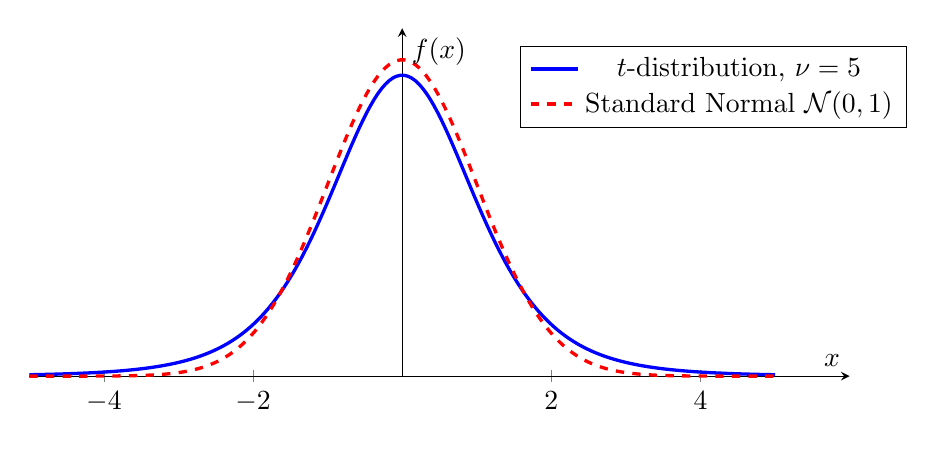
\begin{tikzpicture}
\begin{axis}[
    domain=-5:5,
    samples=200,
    axis lines=middle,
    xlabel={$x$},
    ylabel={$f(x)$},
    legend style={at={(1.07,0.95)}, anchor=north east},
    % grid=both,
    width=12cm,
    height=6cm,
    xtick={-4,-2,0,2,4},
    ytick=\empty,
    enlargelimits=upper,
    clip=false
]

% t-distribution with 5 degrees of freedom
% Formula: Gamma((ν+1)/2) / [sqrt(νπ) * Gamma(ν/2)] * (1 + x^2/ν)^{- (ν+1)/2}
% For ν = 5:
\addplot [blue, very thick] {0.37960669 * (1 + x^2 / 5)^(-3)};
\addlegendentry{\( t \)-distribution, \( \nu = 5 \)}

% Standard normal distribution: 1/sqrt(2pi) * e^{-x^2 / 2}
\addplot [red, dashed, very thick] {1/sqrt(2*pi) * exp(-x^2/2)};
\addlegendentry{Standard Normal \( \mathcal{N}(0,1) \)}


\end{axis}
\end{tikzpicture}
\end{center}
As illustrated in the figure above, the overall shape of the \( t \)-distribution closely resembles that of the standard normal distribution: both are bell-shaped and symmetric about the mean. Like the standard normal distribution, the \( t \)-distribution has a mean of 0. However, its variance depends on the parameter \( \nu \), known as the \textbf{degrees of freedom}. The variance of the \( t \)-distribution is greater than 1 but decreases as \( \nu \) increases, approaching 1 in the limit.

\begin{textbox}
The \( t \)-distribution with \( \nu \) degrees of freedom converges to the standard normal distribution as \( \nu \to \infty \). As a general rule of thumb, the standard normal distribution provides a good approximation to the \( t \)-distribution when the sample size is 30 or larger.
\end{textbox}


\begin{center}
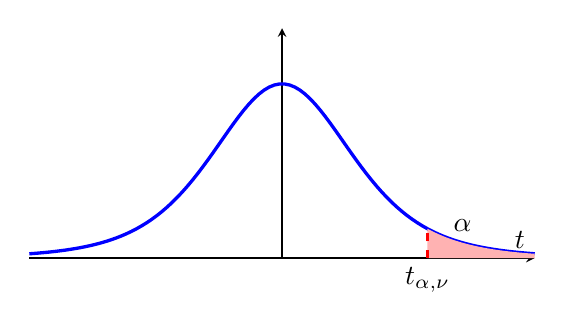
\begin{tikzpicture}
  \begin{axis}[
    domain=-3.5:3.5,
    samples=100,
    axis lines=middle,
    xlabel={$t$},
    width=8cm, height=4.5cm,
    ymin=0, ymax=0.5,
    xtick=\empty,
    ytick=\empty,
    tick style={draw=none},
    clip=false,
  ]
    % Full t_5 PDF curve
    \addplot [very thick, blue] {0.379*(1 + x^2/5)^(-3)};

    % Shaded right tail beyond t_{0.05} ≈ 2.015
    \addplot [
      domain=2.015:3.5,
      samples=100,
      draw=none,
      fill=red!30
    ] {0.379*(1 + x^2/5)^(-3)} \closedcycle;

    % Vertical line at t_{0.05}
    \addplot [red, dashed, thick] coordinates
      {(2.015,0) (2.015,{0.379*(1 + 2.015^2/5)^(-3)})};

    % Annotations
    \node[black, below] at (axis cs:2.015,0) {\(\displaystyle t_{\alpha, \nu}\)};
    \node[black] at (axis cs:2.5,0.07) {\(\alpha\)};
  \end{axis}
\end{tikzpicture}
\end{center}

The critical point \(t_{\alpha, \nu}\) is defined as the point so that the area to its right under the \(t\)-distribution with \(\nu\) degrees of freedom equals \(\alpha\) i.e.
$$P\left(t > t_{\alpha, \nu} \right)= \alpha$$

By symmetry,
\[
t_{1-\alpha, \nu} = -\,t_{\alpha, \nu}
\]
So the critical point for a left‐tail area of \(\alpha\) is \(-t_{\alpha, \nu}\).

\textbf{Example}: Suppose we take a random sample of \( n = 10 \) measurements of battery lifespans (in hours) from a normally distributed population. The data are:

\[
\{42,\ 38,\ 41,\ 39,\ 40,\ 37,\ 44,\ 36,\ 38,\ 40\}
\]

We want to estimate the population mean \( \mu \) and test whether the mean battery life is significantly different from 40 hours.

This is a case where the population standard deviation \( \sigma \) is unknown, so we use the sample standard deviation \( S \), and apply the following test statistic:

\[
t = \frac{\overline{X} - \mu_0}{S / \sqrt{n}}
\]

where:
\begin{itemize}
  \item \( \overline{X} \) is the sample mean,
  \item \( S \) is the sample standard deviation,
  \item \( \mu_0 = 40 \) is the hypothesized population mean,
  \item \( n = 10 \) is the sample size.
\end{itemize}

The statistic \( t \) follows a \( t \)-distribution with \( \nu = n - 1 = 9 \) degrees of freedom under the assumption that the population is normal.

Sample mean:

\[
\overline{X} = \frac{1}{10} (42 + 38 + 41 + 39 + 40 + 37 + 44 + 36 + 38 + 40) = \frac{395}{10} = 39.5
\]

Sample variance:

\[
S^2 = \frac{1}{n - 1} \sum_{i=1}^{10} (X_i - \overline{X})^2 = \frac{1}{9} \sum_{i=1}^{10} (X_i - 39.5)^2 \approx 6.17
\]

\[
S = \sqrt{6.17} \approx 2.48
\]

Test statistic:

\[
t = \frac{\overline{X} - \mu}{S / \sqrt{n}} = \frac{39.5 - 40}{2.48 / \sqrt{10}} \approx \frac{-0.5}{0.784} \approx -0.637
\]

The computed \( t \)-value is approximately \( -0.637 \), and it follows a \( t \)-distribution with \( \nu = 9 \) degrees of freedom. We can compare this value to critical values from the \( t \)-table or compute a \( p \)-value to make inference about \( \mu \).

\section{The Sampling Distribution of the Sample Variance}
When we take a random sample from a population, not only the sample mean but also the \textbf{sample variance}
\[
S^2 = \frac{1}{n - 1} \sum_{i=1}^{n} (X_i - \overline{X})^2
\]
behaves as a random variable. That is, the value of the sample variance \( S^2 \) will vary from one sample to another.

\begin{textbox}
\textbf{Theorem}: If $S^2$ is the variance of a random sample of size $n$ taken (with replacements) from a population of variance $\sigma^2$, then
\[
\mathbb{E}(S^2) = \sigma^2
\]
\end{textbox}

\textbf{Proof}: Let \( X_1, X_2, \dots, X_n \) be a random sample from a population with mean \( \mu \) and variance \( \sigma^2 \). The sample variance is defined as:
\[
S^2 = \frac{1}{n - 1} \sum_{i=1}^{n} (X_i - \overline{X})^2
\]

Now,
\begin{align*}
\sum_{i=1}^{n} (X_i - \overline{X})^2 &= \sum_{i=1}^{n} \left( (X_i - \mu) - (\overline{X} - \mu)\right) ^2\\
&= \sum_{i=1}^{n} (X_i - \mu)^2 - n(\overline{X} - \mu)^2
\end{align*}

Taking expectations on both sides:
\[
\mathbb{E}\left[\sum_{i=1}^{n} (X_i - \overline{X})^2 \right] = \mathbb{E}\left[ \sum_{i=1}^{n} (X_i - \mu)^2 \right] - n \cdot \mathbb{E}\left[(\overline{X} - \mu)^2 \right]
\]

Now, observe:
\begin{align*}
\mathbb{E}\left[\sum_{i=1}^{n} (X_i - \mu)^2 \right] &= \sum_{i=1}^{n} \mathbb{E}(X_i - \mu)^2 = n\sigma^2 \\
\mathbb{E}\left[(\overline{X} - \mu)^2 \right] &= \text{Var}(\overline{X}) = \frac{\sigma^2}{n}
\end{align*}

Therefore:
\[
\mathbb{E}\left[\sum_{i=1}^{n} (X_i - \overline{X})^2 \right] = n\sigma^2 - n \cdot \frac{\sigma^2}{n} = n\sigma^2 - \sigma^2 = (n - 1)\sigma^2
\]

Dividing both sides by \( n - 1 \), we get:
\[
\mathbb{E}(S^2) = \frac{1}{n - 1} \cdot (n - 1)\sigma^2 = \sigma^2
\]
\hfill $\blacksquare$

Thus the expectation value of the sample variance is the population variance. This result illustrates why the term \( n - 1 \) is used in the denominator of the definition of sample variance, rather than \( n \).
But we still don't know the exact shape of the sampling distribution. To describe the exact sampling distribution of \( S^2 \), we require the additional assumption that the population is normally distributed. Under this assumption, the following result holds:


\begin{textbox}
\textbf{Theorem}: If $S^2$ is the variance of a random sample of size $n$ taken from a normal population of variance $\sigma^2$, then the statistic
\[
\chi^2 = \frac{(n - 1)S^2}{\sigma^2}
\]
follows a \textbf{chi-squared distribution} with \( \nu = n - 1 \) degrees of freedom.
\end{textbox}

This theorem tells us how the sample variance \( S^2 \) is distributed around the true population variance \( \sigma^2 \).

\begin{center}
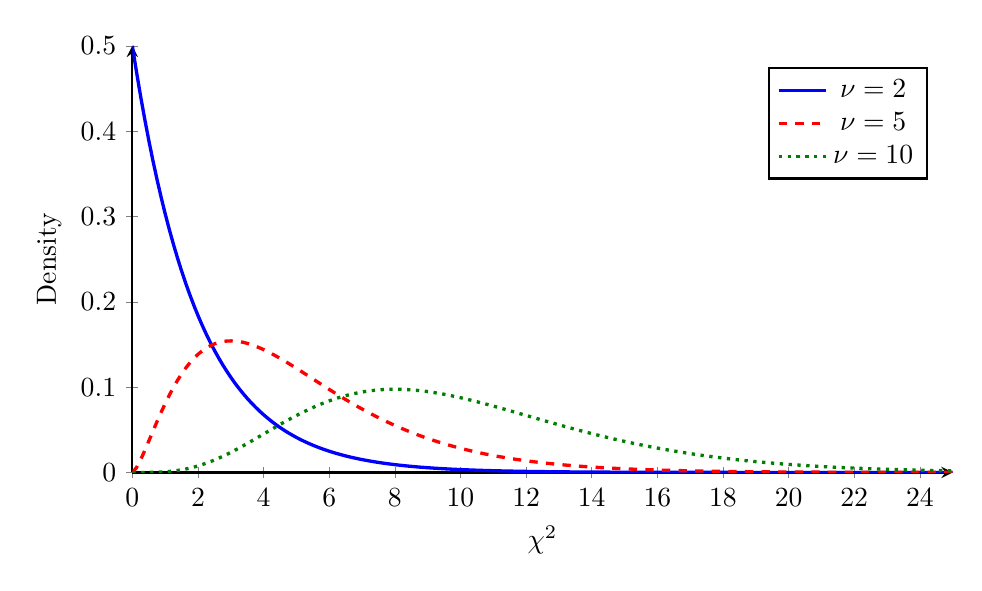
\begin{tikzpicture}
\begin{axis}[
    width=12cm, height=7cm,
    domain=0:25, samples=200,
    axis lines=left,
    xlabel={$\chi^2$},
    ylabel={Density},
    legend style={at={(0.97,0.95)}, anchor=north east},
    % title={\small Chi-Squared Distributions for Different Degrees of Freedom},
    % grid=major,
    thick,
]

% ν = 2: f(x) = (1/2) * exp(-x/2)
\addplot [blue, very thick] {(1/2) * exp(-x/2)};
\addlegendentry{$\nu = 2$}

% ν = 5: f(x) = (1 / (2^{5/2} * Γ(5/2))) * x^{3/2} * exp(-x/2)
% Γ(5/2) = 1.3293..., 2^{5/2} = 5.6568...
% Constant = 1 / (5.6568 * 1.3293) ≈ 0.133
\addplot [red, very thick, dashed] {0.133 * x^(1.5) * exp(-x/2)};
\addlegendentry{$\nu = 5$}

% ν = 10: f(x) = (1 / (2^5 * Γ(5))) * x^4 * exp(-x/2)
% Γ(5) = 24, 2^5 = 32
% Constant = 1 / (32 * 24) = 1 / 768 ≈ 0.0013
\addplot [green!50!black, very thick, dotted] {0.0013 * x^4 * exp(-x/2)};
\addlegendentry{$\nu = 10$}

\end{axis}
\end{tikzpicture}
\end{center}

A Chi-squared distribution has the following properties:
\begin{itemize}
    \item The chi-squared distribution is not symmetric; it is skewed to the right, especially for small degrees of freedom.
    \item As the sample size increases (\( n \to \infty \)), the distribution becomes more symmetric and approaches normality.
    \item The expected value of the distribution is \( \mathbb{E}[\chi^2] = n-1 \).
    \item The critical point \(\chi^2_{\alpha,\nu}\) is defined as a point such that
\[
P\bigl(\chi^2_\nu > \chi^2_{\alpha,\nu}\bigr) \;=\;\alpha
\]
where \(\chi^2_\nu\) denotes a chi-square random variable with \(\nu\) degrees of freedom.
\end{itemize}

\section{Distribution of the Ratio of Two Sample Variances}

A problem closely related to that of finding the distribution of the sample variance is that of determining the distribution of the ratio of the variances of two independent random samples. This problem is of considerable importance because it arises in hypothesis testing situations where we want to assess whether two samples come from populations with equal variances.

\begin{textbox}
\textbf{Theorem}: Let \( S_1^2 \) and \( S_2^2 \) be the sample variances of two independent random samples of sizes \( n_1 \) and \( n_2 \), respectively, drawn from two normal populations with equal variances $\sigma_1^2$ and $\sigma_2^2$ respectively. Then the statistic
\[
F = \dfrac{S_1^2/\sigma_1^2}{S_2^2/\sigma_2^2} = \dfrac{S_1^2/S_2^2}{\sigma_1^2/\sigma_2^2}
\]
follows an $ F $-distribution ($F \sim F_{\nu_1, \nu_2}$) with \( \nu_1 = n_1 - 1 \) and \( \nu_2 = n_2 - 1 \) degrees of freedom.
\end{textbox}
This theorem tells us how the ration of sample variances \( {S_1^2}/{S_2^2} \) is distributed around the true population variance \( {\sigma_1^2}/{\sigma_2^2} \).
% If two populations have the same variance, the sample variances obtained from them should be approximately equal. In such a case, the ratio of the two sample variances should be close to 1.

Properties of $F$-distribution:

\begin{itemize}
	\item The $ F $-distribution is characterized by two parameters:
	\begin{itemize}
		\item \( \nu_1 \): \textbf{numerator degrees of freedom},
		\item \( \nu_2 \): \textbf{denominator degrees of freedom}.
	\end{itemize}

	\item Reciprocal property:
	\begin{textbox}
		If $X \sim F_{\nu_1, \nu_2}$, then the reciprocal of $X$ i.e. $Y = \dfrac{1}{X} \sim F_{\nu_2, \nu_1}$.
	\end{textbox}

	\item The critical point \(F_{\alpha; \nu_1, \nu_2}\) is defined as a point such that
	\[
	P\bigl(X > F_{\alpha; \nu_1, \nu_2}) \;=\;\alpha
	\]
	Equivalently\footnote{This inverse relationship is maintained because $f(x) = \dfrac{1}{x}$ is a \textbf{strictly decreasing bijection} on \((0,\infty)\). Hence the event \(\{A < B\}\) is is exactly the same as the event \(\{f(A) > f(B)\}\) or the event \(\left\{\dfrac{1}{A} > \dfrac{1}{B}\right\}\).},
	\[
	P\left( \dfrac1X < \dfrac1{F_{\alpha;\nu_1,\nu_2}}\right) =\alpha
	\]
	But \(\dfrac1X = Y\sim F_{\nu_2,\nu_1}\).  Under the upper‑tail critical point definition convention, if \(F_{1-\alpha;\nu_2,\nu_1}\) is the critical value satisfying
	\[
	P\bigl(Y > F_{1-\alpha;\nu_2,\nu_1}\bigr)=1-\alpha
	\]
	then equivalently
	\[
	P\bigl(Y \le F_{1-\alpha;\nu_2,\nu_1}\bigr)=\alpha
	\]
	Comparison with \(P(Y<1/F_{\alpha;\nu_1,\nu_2})=\alpha\) shows
	\[
	\frac1{F_{\alpha;\nu_1,\nu_2}}
	\;=\;
	F_{1-\alpha;\nu_2,\nu_1}
	\]
	and hence
	\begin{textbox}
		\[
		F_{\alpha;\nu_1,\nu_2}
		\;=\;
		\frac1{F_{1-\alpha;\nu_2,\nu_1}}
		\]
	\end{textbox}
\end{itemize}




\section{The Sampling Distribution of the Sample Proportion}
Let $X_1, X_2, \dots, X_n$ be a random sample from a Bernoulli population with proportion parameter $p$. Then the \textbf{sample proportion} is defined as:
\[
\hat{p} = \frac{1}{n} \sum_{i=1}^{n} X_i = \frac{X}{n}
\]
where $X$ is the number of successes in the sample of size $n$. Since \( X \) is a binomial random variable with parameters \( n \) and \( p \), i.e., \( X \sim \text{Bin}(n, p) \), it follows that:
\begin{itemize}
    \item The mean of \( \hat{p} \) is:
    \[
    \mathbb{E}\left( \hat{p}\right) = \frac{1}{n}\mathbb{E}(X) = \frac{np}{n} = p
    \]
    \item The variance of \( \hat{p} \) is:
    \[
    \text{Var}(\hat{p}) = \frac{1}{n^2}\text{Var}(X) = \frac{npq}{n^2}=\frac{pq}{n}, \quad \text{where } q = 1 - p
    \]
\end{itemize}

\begin{textbox}
    \textbf{Theorem}: For large sample size \( n \), the distribution of sample proportion \( \hat{p} \) can be approximated by a normal distribution according to the Central Limit Theorem:
    \[
    \hat{p} \sim \mathcal{N}\left(p, \frac{pq}{n}\right)
    \]
\end{textbox}
This approximation is generally considered valid when both \( np \geq 5 \) and \( nq \geq 5 \).

The standardized form of \( \hat{p} \) is:
\[
\frac{\hat{p} - p}{\sqrt{pq/n}}
\]
which follows the standard normal distribution $\mathcal{N}\left(0, 1\right)$ for large sample.

\textbf{Example}: Suppose the true population proportion is \( p = 0.6 \) and a sample of size \( n = 100 \) is taken. Then:
\begin{align*}
\mathbb{E}\left( \hat{p}\right) &= 0.6 \\
\textrm{Var}(\hat{p}) &= \frac{0.6 \cdot 0.4}{100} = 0.0024
\end{align*}
Thus, the distribution of \( \hat{p} \) can be approximated as \( N(0.6, 0.0024) \).




\chapter{Theory of Estimation}

\section{Introduction}
Estimation is a fundamental component of \textbf{statistical inference}, which deals with drawing conclusions about population parameters from the analysis of sample data. There are two primary types of statistical inference:

\begin{enumerate}
    \item \textbf{Estimation of parameters}: The true value of a population parameter is an unknown constant. The goal of estimation is to make informed guesses about this parameter using sample data, along with an assessment of the accuracy of these guesses.

    \item \textbf{Hypothesis testing}: Sometimes, preliminary or tentative information about a population parameter is available. The objective of hypothesis testing is to use sample data to either support or reject such information about the parameter.
\end{enumerate}

In this chapter, we focus on the first type—{estimation of parameters}. Hypothesis testing will be addressed in the next chapter.

Statistical estimation techniques are broadly classified into two categories:

\begin{enumerate}
    \item \textbf{Point estimation}: A point estimation provides a single best guess of the unknown population parameter.

    \item \textbf{Interval estimation}: An interval estimation gives a range of plausible values for the parameter, along with a specified level of confidence that the interval contains the true value.
\end{enumerate}

Both point and interval estimation play crucial roles in quantifying uncertainty and guiding decision-making in the presence of incomplete information.


\section{Point Estimation}
Let $\theta$ ne an unknown parameter (e.g. the population mean) associated with a particular variable. For estimating $\theta$ on the basis of random samples $X_1, X_2, \dots, X_n$, we may use a particular statistic $ T $. This statistic $T$ is called the \textbf{point estimator} of $\theta$ and the value of $T$ obtained from a given sample is referred to as an \textbf{estimate} of $\theta$.

\textbf{Example}: When we estimate the population mean $\theta = \mu$, the most intuitive estimator is the sample mean $\overline{X} = \dfrac{1}{N}\sum_{i=1}^{n}X_i$. Similarly sample variance (\( S^2 \)) estimates population variance (\( \sigma^2 \)) and sample proportion (\( \hat{p} \)) estimates population proportion (\( p \))


\subsection{Desirable Properties of a Good Estimator}
There are often multiple point estimates available for any given parameter. So it is important to develop some evaluating criteria to judge the performance of each estimator and compare their performance. A good estimator should possess following desirable properties that make it reliable in estimating the true parameter value.

\begin{enumerate}
    \item \textbf{Unbiasedness}:
    \begin{textbox}
    An estimator \( T \) is said to be an \textbf{unbiased} estimator of $\theta$ if
    \[
        \mathbb{E}(T) = \theta
        \]
    \end{textbox}
    Otherwise, $T$ is said to be biased. The \textbf{bias} ($\mathcal{B}$) is given by
    $$\mathcal{B} = \mathbb{E}(T) - \theta$$

    \textbf{Example}: The sample mean $\overline{X}$ and sample variance $S^2$ are unbiased estimator of the population mean $\mu$ and population variance $\sigma^2$ respectively, because
    $$\mathbb{E}\left( \overline{X}\right) = \mu, \quad \mathbb{E}\left( S^2\right) = \sigma^2$$

    \begin{textbox}
    The \textbf{mean-square-error} of the estimator $T$, denoted by $\textrm{MSE}(T)$ is defined as
        $$\mathrm{MSE}(T) = \mathbb{E}\left[\left( T-\theta\right) ^2\right]$$
    \end{textbox}

    MSE measures, on average, how close an estimator comes to the true value of the parameter.

    \begin{textbox}
    \textbf{Theorem}: Let \( T \) be an estimator of a population parameter \( \theta \). Then, the {Mean Squared Error (MSE)} of \( T \) is given by:
    \[
    \mathrm{MSE}(T) = \mathrm{Var}(T) + \mathcal{B}^2(T)
    \]
    \end{textbox}
    \textbf{Proof}:
    \begin{align*}
    \mathrm{MSE}(T) &= \mathbb{E}\left[(T - \theta)^2\right] \\
    &= \mathbb{E}\left[\left((T - \mathbb{E}(T)) + (\mathbb{E}(T) - \theta)\right)^2\right] \\
    &= \mathbb{E}\left[(T - \mathbb{E}(T))^2 + 2(T - \mathbb{E}(T))(\mathbb{E}(T) - \theta) + (\mathbb{E}(T) - \theta)^2\right] \\
    &= \mathbb{E}[(T - \mathbb{E}(T))^2] + \underbrace{2(\mathbb{E}(T) - \mathbb{E}(T))}_{= 0}\mathbb{E}\left( T - \mathbb{E}(T)\right)  + (\mathbb{E}(T) - \theta)^2 \\
    &= \mathrm{Var}(T) + \mathcal{B}^2(T)
    \end{align*}
    \hfill $\blacksquare$

    For an unbiased estimator $\mathcal{B} = 0$, and therefore $\mathrm{MSE}(T) = \mathrm{Var}(T)$.

    In this context, the \textbf{standard error (SE)} of $T$ is defined as the standard deviation of $T$ i.e. $ \sqrt{\operatorname{Var}(T)} $ which is diffierent from MSE($T$).

    \item \textbf{Consistency}:

    It is desirable that the estimator should behave more and more satisfactorily as the sample size $n$ becomes larger. Consistency provides the criteria.

    \begin{textbox}
    An estimator \(T_n\) (from a sample of size $n$) of a parameter \(\theta\) is said to be \textbf{consistent} if, as the sample size \(n\) grows, \(T_n\) converges in probability to the true parameter value. Which means that for every \(\varepsilon > 0\),
        \[
        P\bigl(|T_n - \theta| > \varepsilon\bigr) \to 0 \quad \text{as} \quad n \to \infty
        \]
    \end{textbox}

    Consistency as defined above is sometimes called \textbf{weak consistency}. If we replace convergence in probability with almost sure convergence, i.e. $$ P\left(\lim_{n \to \infty}T_n - \theta\right) = 1 \quad \text{as} \quad n \to \infty, $$
    then the estimator is said to be \textbf{strongly consistent}\footnote{\textbf{Weak consistency} says “in the long run, most of your estimates will be good,” but allows for occasional wildly bad estimates—even when \(n\) is very large.

    \textbf{Strong consistency} rules out even those rare catastrophes: it guarantees that once you’ve accumulated enough data, your estimator will stay arbitrarily close to \(\theta\) for every subsequent sample.
    }.

    \begin{textbox}
    \textbf{Sufficient Conditions for Consistency}: An estimator \(T_n\) of a parameter \(\theta\) is said to be {consistent} if it satisfies the following two conditions:
    \begin{enumerate}
      \item If $T_n$ is an \textit{asymptotically unbiased} estimator of $\theta$ i.e.
      \[
        \mathbb{E}(T_n) \to \theta \quad \text{as } n \to \infty
      \]
      \item The variance of estimator $ T_n $ decreases with increasing sample size i.e.
      \[
        \mathrm{Var}(T_n) \to 0 \quad \text{as } n \to \infty
      \]
    \end{enumerate}
    \end{textbox}
    \textbf{Proof}: By Chebyshev’s inequality, if both conditions hold, then
    \begin{align*}
    P\bigl(|T_n - \theta| \ge \varepsilon\bigr)
        &\le \frac{\mathbb{E}(T_n-\theta)^2}{\varepsilon^2}, \quad \text{for every } \varepsilon > 0\\
        &= \frac{1}{\varepsilon^2}\left(\mathbb{E}\left[\left( T_n-\mathbb{E}(T_n)\right) + \left(\mathbb{E}(T_n)-\theta) \right)  \right]^2\right)\\
        &= \frac{1}{\varepsilon^2}\left(\underbrace{\mathbb{E}\left( T_n-\mathbb{E}(T_n)\right)^2}_{\mathrm{Var}(T_n)} +\left(\mathbb{E}(T_n)-\theta)\right) ^2 \right) \\
        &= \frac{1}{\varepsilon^2}\left( \mathrm{Var}(T_n)+\left(\mathbb{E}(T_n)-\theta)\right) ^2
        \right)\\
        &\to 0 \quad \text{as} \quad n \to \infty
     \end{align*}
    \hfill $\blacksquare$

    An estimator can be consistent even if it is biased for each finite \(n\), provided the bias vanishes as \(n \to \infty\).

    \textbf{Example}: Let \(X_1, X_2, \dots, X_n\) be i.i.d.\ with mean \(\mu\) and finite variance \(\sigma^2\). The sample mean
    \[
    \overline{X}_n = \frac{1}{n}\sum_{i=1}^n X_i
    \]
    satisfies
    \[
    \mathbb{E}[\overline{X}_n] = \mu,
    \qquad
    \mathrm{Var}(\overline{X}_n) = \frac{\sigma^2}{n} \;\longrightarrow\; 0.
    \]
    Hence, by the two conditions above, \(\overline{X}_n\) is a consistent estimator of \(\mu\).

    \item \textbf{Efficiency}:

    \begin{textbox}
    Among all unbiased estimators, the one with the smallest variance is said to be most \textbf{efficient}.
    \end{textbox}

    Unbiasedness is certainly a desirable property for point estimators but the criterion of unbiasedness does not generally provide a unique statistic for a given problem of estimation. For example, for symmetric population distribution, the sample median is also unbiased estimator for all sample sizes. Clearly, we need a further criterion to decide among different candidates.

    One natural refinement is to compare their variances which measures the spread
     of the sampling distribution. Although both the sample mean and the sample median of a normal population are unbiased and have bell‐shaped sampling distributions centered at \(\mu\), the variance of the sample mean is
        \[
        \mathrm{Var}\bigl(\overline{X}\bigr) = \frac{\sigma^2}{n},
        \]
        whereas the variance of the sample median is approximately
        \[
        \mathrm{Var}\bigl(X_{\text{median}}\bigr) \approx 1.5708\,\frac{\sigma^2}{n}.
        \]
        Because the mean’s distribution is more concentrated around \(\mu\), it will, on average, provide estimates closer to the truth. In other words, among unbiased estimators we favor the one with the smaller variance—and we call it, the most \textbf{efficient} estimator.

        This leads to the concept of the \emph{Minimum Variance Unbiased Estimator (MVUE)}:

        \begin{textbox}
        The unbiased estimator $T^*$ is a \textbf{Minimum Variance Unbiased Estimator (MVUE)} of a parameter if it has the smallest variance among all unbiased estimators of the parameter.

        Formally, if \(\mathcal{U}\) is the class of all unbiased estimators of \(\theta\), then the MVUE \(T^*\) satisfies
                \[
                \mathrm{Var}\bigl(T^*\bigr) \;=\; \inf_{T \in \mathcal{U}} \mathrm{Var}\bigl(T\bigr)
                \]
            \end{textbox}

        If two unbiased estimators $T_1$ and $T_2$ estimate the same parameter $\theta$, the \textbf{relative efficiency} of $T_1$ with respect to $T_2$ is defined as:

        \begin{textbox}
        \[
                \text{Relative Efficiency} = \frac{\operatorname{Var}(T_2)}{\operatorname{Var}(T_1)}.
                \]
        \end{textbox}

        An estimator is more efficient if it has a smaller variance. If the relative efficiency is close to 1, both estimators are equally good in terms of variance.

    \item \textbf{Sufficiency}:

    \begin{textbox}
    A statistic is said to be \textbf{sufficient} for a parameter if it captures all the information in the sample about that parameter.
    \end{textbox}

    Sufficiency is a key concept because it allows us to summarize the data without losing any relevant information about the parameter of interest.

    Let $\mathbf{X} = (X_1, X_2, \ldots, X_n)$ be a random sample from a distribution with conditional joint probability density function (or joint probability mass function) $$f_{\mathbf{X}}(x_1, x_2, \dots, x_n ; \theta),$$ where $\theta$ is an unknown parameter\footnote{\textbf{Why we write the joint PDF in the form $f_{\mathbf{X}}(x_1, x_2, \dots, x_n; \theta)$ and not $f_{\mathbf{X}}(x_1, x_2, \dots, x_n \mid \theta)$}?

    \noindent Because in frequentist statistics, the parameter $\theta$ is treated as a fixed (but unknown) constant, while the data $\mathbf{X} = (X_1, X_2, \dots, X_n)$ are considered random variables. Therefore, we write the joint probability density (or mass) function as
        $ f_{\mathbf{X}}(x_1, x_2, \dots, x_n; \theta) $
        which emphasizes that this is a function of the data and a given fixed parameter.

        On the other hand, the notation $f_{\mathbf{X}}(x_1, x_2, \dots, x_n \mid \theta)$ is typically reserved for conditional distributions, where $\theta$ is treated as a random variable—as in Bayesian statistics. In the frequentist context, $\theta$ is not random, so we avoid the conditional notation.}.

   \begin{textbox}
    A statistic $T(\mathbf{X})$ is said to be \textbf{sufficient} for $\theta$ if the conditional distribution of $X_1,X_2,\dots, X_n$ given $T(\mathbf{X}) = t$ does not depend on $\theta$. That is,
       \[
       f_{\mathbf{X}}(x_1, x_2, \dots, x_n \mid T = t; \theta) = f_{\mathbf{X}}(x_1, x_2, \dots, x_n \mid T = t)
       \]
       $ \text{for all } \theta $.
   \end{textbox}

   In other words, once you know \(T = t\), the probability (or density) of seeing any particular arrangement of the raw observations does not depends on \(\theta\). After you condition on \(T = t\), you look at the probability of different possible datasets that all share that same \(T\)-value. If that conditional probability still changes with \(\theta\), then those leftover items are carrying extra clues about \(\theta\).


   A useful tool to verify sufficiency is the {Neyman–Fisher Factorization Theorem}, which states:

    \begin{textbox}
    \textbf{Neyman–Fisher Factorization Theorem}: A necessary and sufficient condition for the statistic $T(\textbf{X})$ to be a sufficient statistic for $\theta$ is that the joint PDF (or joint PMF) function of the sample can be factorized as:
        \[
         f_{\mathbf{X}}(x_1, x_2, \ldots, x_n; \theta) = g(T;\theta) \cdot h(x_1, x_2, \ldots, x_n)
        \]
        where
        \begin{itemize}
            \item $g(T;\theta)$ is a function that depends on the data
             $ (x_1, x_2, \ldots, x_n) $ only through the function $T(x_1, x_2, \ldots, x_n)$.
            \item $h(x_1, x_2, \ldots ,x_n)$ is a function of the data that does not depend on the parameter $\theta$.
        \end{itemize}
    \end{textbox}

    \bigskip

    \textbf{Example}: Let \(X_1, X_2, \dots, X_n\) be independent Bernoulli random variables with common success probability \(p\). Therefore
    \[
    X_i =
    \begin{cases}
    1, & \text{with probability } p\\
    0, & \text{with probability } 1 - p
    \end{cases}
    \]

    We wish to show that the total proportion of successes in the sample,
    \[
    T(\mathbf{X}) \;=\; \frac{1}{n}\sum_{i=1}^n X_i
    \]
    is a sufficient statistic for \(p\).


    The joint probability mass function of the sample \(\textbf{X} = (X_1,X_2,\dots,X_n)\) is
    \[
    f_{\textbf{X}}(x_1,x_2,\dots,x_n;\,p) = \prod_{i=1}^{n} p^{x_i}(1-p)^{1-x_i}
    =
    p^{\sum_{i=1}^n x_i}
    \,(1 - p)^{\,n - \sum_{i=1}^n x_i}
    \]

    Observe that this can be written in the form
    \[
    f(x_1,x_2,\dots,x_n;\,p)
    =
    \underbrace{p^{nT(\textbf{x})} \,(1-p)^{\,n - nT(\textbf{x})}}_{g\bigl(T(\textbf{x}),p\bigr)}
    \;\times\;
    \underbrace{1}_{h(x)}
    \]
    where
    \[
    T(\textbf{x}) = \sum_{i=1}^n x_i
    \]
    Here:
    \begin{itemize}
      \item \(g\bigl(T(\textbf{x});p\bigr) = p^{T(\textbf{x})} (1-p)^{\,n - T(\textbf{x})}\) depends only on the statistic \(T(\textbf{x})\) and the parameter \(p\).
      \item \(h(x) = 1\) depends on the full data \(\mathbf{x} = (x_1,x_2,\dots,x_n)\) but not on \(p\).
    \end{itemize}

    Therefore, the statistic \(T(\textbf{X})=\frac{1}{n}\sum_{i=1}^n X_i\) is sufficient for the parameter \(p\).

    \bigskip

    \textbf{Example}: Let \(X_1, X_2, \dots, X_n\) be independent random variables drawn from a normal distribution with unknown mean \(\mu\) and known variance \(\sigma^2\).  That is,
    \[
    X_i \sim \mathcal{N}(\mu,\sigma^2),
    \]
    so each density is
    \[
    f_{X_i}(x_i ; \mu)
    =
    \frac{1}{\sqrt{2\pi\,\sigma^2}}
    \exp\Bigl(-\tfrac{1}{2\sigma^2}(x_i - \mu)^2\Bigr)
    \]

    We wish to show that the sample mean
    \[
    T(\mathbf{X}) \;=\; \frac{1}{n}\sum_{i=1}^n X_i
    \]
    is a sufficient statistic for \(\mu\).

    The joint density of the sample \(\mathbf{X}=(X_1,X_2,\dots,X_n)\) is
    \[
    \begin{aligned}
    f_{\mathbf{X}}(x_1,x_2,\dots,x_n ; \mu)
    &=
    \prod_{i=1}^{n}
    \frac{1}{\sqrt{2\pi\,\sigma^2}}
    \exp\!\left( -\tfrac{1}{2\sigma^2}(x_i - \mu)^2\right) \\
    &=
    (2\pi\,\sigma^2)^{-\tfrac{n}{2}}
    \exp\!\left( -\tfrac{1}{2\sigma^2}\sum_{i=1}^n (x_i - \mu)^2\right)
    \end{aligned}
    \]

    Rewrite the exponential term:
    \[
    \sum_{i=1}^n (x_i - \mu)^2
    =
    \sum_{i=1}^n x_i^2
    \;-\;2\mu\sum_{i=1}^n x_i
    \;+\;n\,\mu^2 = \sum_{i=1}^n x_i^2\;-\;n\,\mu^2
    \]
    Thus
    \[
    \exp\!\left( -\tfrac{1}{2\sigma^2}\sum_i (x_i - \mu)^2\right)
    =
    \exp\!\left( -\tfrac{1}{2\sigma^2}\sum_i x_i^2\right)
    \;\times\;
    \exp\!\left( \tfrac{\mu}{\sigma^2}\sum_i x_i \;-\;\tfrac{n\mu^2}{2\sigma^2}\right)
    \]
    Hence the joint density factors as
    \[
    \begin{aligned}
    f_{\textbf{X}}(x_1,x_2,\dots,x_n ; \mu)
    &=
    \underbrace{%
    \exp\!\left( \tfrac{n\mu}{\sigma^2}\,T(\textbf{x})
         \;-\;\tfrac{n\mu^2}{2\sigma^2}\right)
    }_{g\bigl(T(\textbf{x}),\mu\bigr)}
    \;\times\;
    \underbrace{%
    (2\pi\,\sigma^2)^{-\tfrac{n}{2}}
    \exp\!\left( -\tfrac{1}{2\sigma^2}\sum_i x_i^2\right)
    }_{h(x)}
    \end{aligned}
    \]
    where \(T(\textbf{x})=\sum_{i=1}^n x_i\). Therefore, by the Neyman–Fisher factorization theorem, because the statistic
    \(\displaystyle T(\mathbf{X})=\frac{1}{n}\sum_{i=1}^n X_i\) is sufficient for \(\mu\).

    \bigskip

    \textbf{Example}: Let \( X_1 \) and \( X_2 \) be two independent and identically distributed random variables from the Poisson distribution with parameter \(\lambda > 0\), i.e.,
    \[
    X_1, X_2 \overset{iid}{\sim} \text{Poisson}(\lambda)
    \]
    The probability mass function of a Poisson random variable is given by
    \[
    P(X_i = x_i; \lambda) = \frac{e^{-\lambda} \lambda^{x_i}}{x_i!}, \quad x_i = 0, 1, 2, \dots
    \]
    Since \(X_1\) and \(X_2\) are independent, the joint PMF of the sample is
    \[
    p_{X_1,X_2}(x_1, x_2 ; \lambda) = \frac{e^{-\lambda} \lambda^{x_1}}{x_1!} \cdot \frac{e^{-\lambda} \lambda^{x_2}}{x_2!}
    = \frac{e^{-2\lambda} \lambda^{x_1 + x_2}}{x_1! x_2!}
    \]

    Now consider the statistic
    \[
    T = X_1 + 2X_2
    \]

    To apply the Neyman–Fisher Factorization Theorem, we attempt to factor the joint PMF in the form
    \[
    p_{X_1,X_2}(x_1, x_2 ; \lambda) = g\bigl(T(x_1, x_2), \lambda\bigr) \cdot h(x_1, x_2)
    \]
    i.e., express the \(\lambda\)-dependence entirely through the statistic \(T\).

    However, in our case the joint PMF is
    \[
    p_{X_1,X_2}(x_1, x_2 ; \lambda) = \frac{e^{-2\lambda} \lambda^{x_1 + x_2}}{x_1! x_2!} = \frac{e^{-2\lambda} \lambda^{T(x_1, x_2) - x_2}}{x_1! x_2!}
    \]
    where the \(\lambda\)-dependent part is \(\lambda^{T(x_1, x_2) - x_2}\), not only a function of $T(x_1, x_2)$ but also a function of $x_2$.
    Therefore, the statistic \(T = X_1 + 2X_2\) is not sufficient.


\end{enumerate}


\section{Maximum Likelihood Estimation (MLE)}

{Maximum Likelihood Estimation (MLE)} is one of the most widely used methods for estimating the parameters of a statistical model. The basic idea is to choose the parameter values that make the observed data most probable.

Let \(\textbf{X} = ( X_1, X_2, \dots, X_n) \) be a random sample from a population with joint probability density function (or probability mass function) \( f_{\textbf{X}}(x_1, x_2, \dots, x_n ; \theta) \), where \( \theta \) is the unknown parameter to be estimated. Given $\textbf{x} = (x_1, x_2, \dots, x_n)$, it may be looked upon as a function of $\theta$, called the \textbf{likelihood function} of $\theta$ and is denoted by $L(\theta)$.
\[
L(\theta) = f_{\textbf{X}}(x_1, x_2, \dots, x_n ; \theta)
\]

The value of \( \theta \) that maximizes this function is called the \textbf{maximum likelihood estimator (MLE)} of \( \theta \):
\[
\hat{\theta} = \arg\max_{\theta} L(\theta)
\]

In practice, it is often more convenient to work with the \textbf{log-likelihood function}:
\[
\log L(\theta) = \log f_{\textbf{X}}(x_1, x_2, \dots, x_n ; \theta)
\]
Maximizing the log-likelihood yields the same estimator as maximizing the likelihood.

\subsubsection*{Example: Poisson distribution}

Suppose \( X_1, X_2, \dots, X_n \) are i.i.d. from a Poisson distribution with parameter \( \lambda > 0 \). The PMF for the Poisson distribution is:
\[
f(x; \lambda) = \frac{e^{-\lambda} \lambda^x}{x!}, \quad x = 0, 1, 2, \dots
\]

The likelihood function is:
\begin{align*}
L(\lambda) &= f_{\textbf{X}}(x_1, x_2, \dots, x_n ; \lambda)\\
&= \prod_{i=1}^n f(x_i ; \lambda) = \prod_{i=1}^n \frac{e^{-\lambda} \lambda^{x_i}}{x_i!} \\
&= e^{-n\lambda} \lambda^{\sum_i x_i} \prod_{i=1}^n \frac{1}{x_i!}
\end{align*}

The log-likelihood is:
\[
\log L(\lambda) = -n\lambda + \left(\sum_i x_i\right) \log \lambda - \sum_i \log(x_i!)
\]

Differentiating and setting the derivative to zero:
\[
\frac{d}{d\lambda}\log L(\lambda) = -n + \frac{1}{\lambda}\sum_i x_i = 0 \Rightarrow \hat{\lambda}  = \frac{1}{n} \sum_i x_i = \overline{x}
\]

Hence, the MLE of $\lambda$ is $\hat{\lambda} = \overline{X}$.

\subsubsection*{Example: Normal distribution}

Assume \( X_1, X_2, \dots, X_n \overset{iid}{\sim} N(\mu, \sigma^2) \). The PDF is:
\[
f(x; \mu, \sigma^2) = \frac{1}{\sqrt{2\pi\sigma^2}} \exp\left( -\frac{(x - \mu)^2}{2\sigma^2} \right)
\]

Likelihood function:
\[
L(\mu, \sigma^2) = \prod_{i=1}^{n}f(x_i; \mu, \sigma) =  (2\pi\sigma^2)^{-\tfrac{n}{2}} \exp \left( - \frac{1}{2\sigma^2} \sum_{i=1}^n (x_i - \mu)^2\right)
\]
Log-likelihood function:
\[
\log L(\mu,\sigma^2)= -\frac{n}{2} \log(2\pi\sigma^2) - \frac{1}{2\sigma^2} \sum_{i=1}^n (x_i - \mu)^2
\]


\begin{enumerate}[label=(\roman*)]
\item \textbf{Case 1: \( \mu \) unknown, \( \sigma \) known ($=\sigma_0$)}

Log-likelihood function:
\[
\log L(\mu) = -\frac{n}{2} \log(2\pi\sigma_0^2) - \frac{1}{2\sigma_0^2} \sum_{i=1}^n (x_i - \mu)^2
\]

Taking derivative and setting to zero:
\[
\frac{d}{d\mu}\log L(\mu) = \frac{1}{\sigma_0^2} \sum_{i=1}^n (x_i - \mu) = 0 \Rightarrow \hat{\mu} = \overline{x}
\]

Hence, the MLE of $\mu$ is $\hat{\mu} = \overline{X}$.

\item \textbf{Case 2: \( \mu \) known ($=\mu_0$), \( \sigma \) unknown}

Log-likelihood:
\[
\log L(\sigma^2) = -\frac{n}{2} \log(2\pi\sigma^2) - \frac{1}{2\sigma^2} \sum_i (x_i - \mu_0)^2
\]

Taking derivative w.r.t. \( \sigma^2 \) and setting to zero:
\begin{align*}
\frac{d}{d\sigma^2}\log L(\sigma^2) = -\frac{n}{2\sigma^2}+\frac{1}{2\sigma^4}\sum_i (x_i - \mu_0)^2= 0
\end{align*}
\[
\Rightarrow \hat{\sigma}^2 = \frac{1}{n} \sum_i (x_i - \mu_0)^2
\]

Hence, the MLE of $\sigma^2$ is $\hat{\sigma^2} = \frac{1}{n} \sum_i (x_i - \mu_0)^2$.

\item \textbf{Case 3: \( \mu \) and \( \sigma \) both unknown}

Log-likelihood:
\[
\log L(\mu,\sigma^2) = -\frac{n}{2} \log(2\pi\sigma^2) - \frac{1}{2\sigma^2} \sum_i (x_i - \mu)^2
\]

Taking partial derivatives and solving the system:
\begin{align*}
\frac{\partial}{\partial \mu} \log L(\mu,\sigma^2) = 0 &\Rightarrow \hat{\mu} = \overline{x} \\
\frac{\partial}{\partial \sigma^2} \log L(\mu,\sigma^2) = 0 &\Rightarrow \hat{\sigma}^2 = \frac{1}{n} \sum_i (x_i - \overline{x})^2
\end{align*}
Thus, the MLEs for \( \mu \) and \( \sigma^2 \) are the sample mean $\overline{X}$ and sample variance $\frac{1}{n} \sum_i (x_i - \overline{x})^2$ (without Bessel's correction), respectively.

\end{enumerate}

It is important to note that the maximum likelihood estimator (MLE) of the population variance \( \sigma^2 \) is \textbf{not an unbiased estimator}. The MLE is given by
\[
\hat{\sigma}^2 = \frac{1}{n} \sum_{i=1}^n (X_i - \overline{X})^2,
\]
where \( \overline{X} \) is the sample mean. Buit we have already seen that the unbiased estimator of $\sigma^2$ is:
\[
S^2 = \frac{1}{n-1} \sum_{i=1}^n (X_i - \overline{X})^2 = \frac{n-1}{n}\hat{\sigma}^2
\]

The MLE estimator tends to underestimate the true variance.


\section{Bayesian Estimation}

Bayesian estimation is a method of statistical inference in which the unknown parameter $\theta$ is modeled as a random variable $\Theta$ with a probability distribution $\pi_{\Theta}(\theta)$, known as the \textbf{prior distribution}. It is  intended to reflect our knowledge of the parameter $\theta$, before we gather data.

Let \(\mathbf{X} = (X_1, X_2, \dots, X_n)\) be random variables representing the observations in the sample data with joint PDF (PMF) given $\Theta = \theta$ is given by $f_{\textbf{X}}(\textbf{x} \mid \theta)$ which is also known as the \textbf{likelihood}. When data $ \textbf{X}=\textbf{x} $ are observed, the extra information about $ \theta $ is combined with the prior distribution to obtain the \textbf{posterior distribution} $\pi_{\Theta}(\theta \mid \textbf{x})$ for $ θ $ given $ \textbf{X}=\textbf{x} $ using Bayes theorem as follows:

\[
\pi_{\Theta}(\theta\mid\mathbf{X}) = \frac{f_{\textbf{X}}(\mathbf{x}\mid\theta) \pi_{\Theta}(\theta)}{f_{\textbf{X}}(\mathbf{x})}
\]

where,
\[
f_{\textbf{X}}(\mathbf{x}) =
\begin{cases}
\displaystyle
\sum_{\theta} f_{\textbf{X}}(\mathbf{x} \mid \theta) \pi_{\Theta}(\theta),
& \text{in the discrete case},\\[8pt]
\displaystyle
\int_{-\infty}^{\infty} f_{\textbf{X}}(\mathbf{x} \mid \theta) \pi_{\Theta}(\theta) \, d\theta,
& \text{in the continuous case}.
\end{cases}
\]

Thus,
\[
\underbrace{\pi_{\Theta}(\theta \mid \textbf{x})}_{\text{posterior}}
\;\propto\;
\underbrace{f_{\textbf{X}}(\textbf{x} \mid \theta)}_{\text{likelihood}}
\;\times\;
\underbrace{\pi_{\Theta}(\theta)}_{\text{prior}}
\]

In practice the constant of proportionality chosen in such a way that it makes the total mass of the posterior distribution equal to one. The posterior distribution reflects our updated belief about the parameter after seeing the data.

\textbf{Example}: Suppose you have three coins in your pocket:

\begin{itemize}
    \item Coin 1: Biased in favour of tails with head probability $\theta = 0.25$
    \item Coin 2: A fair coin with $\theta = 0.5$
    \item Coin 3: Biased in favour of heads with $\theta = 0.75$
\end{itemize}

You randomly select one coin and flip it once. You observe a head. What is the posterior probability that you chose Coin 3?

This is a classic example of Bayesian inference with a discrete parameter space.
The \textbf{population} consists of three types of coins, each with a different probability of producing a head: $\theta \in \{0.25, 0.5, 0.75\}$.


We assume one of these coins is selected at random. The \textbf{sample} is a single coin toss from the selected coin, which results in observing a head.
Using this one data point, we update our belief (prior distribution) over the possible values of $\theta$ to obtain a posterior distribution.

Let $X = 1$ denote the event that you observe a head, and $X = 0$ for a tail.

Let $\theta$ denote the probability of heads. Then $\theta \in \{0.25, 0.5, 0.75\}$.

The \textbf{prior probabilities} are:
\[
P(\theta = 0.25) = P(\theta = 0.5) = P(\theta = 0.75) = \frac{1}{3}
\]
Because the probability of selecting any coin at random is same before we have the knowledge of the sample observation.

The \textbf{likelihood} is given by the Bernoulli probability mass function:
\[
P(X = x \mid \theta) = \theta^x (1 - \theta)^{1 - x}
\]
Since we observed $X = 1$, the likelihood becomes $P(X=1 \mid \theta) = \theta$.

We now calculate the unnormalized and normalized \textbf{posterior probabilities} using Bayes' Theorem:

\[
\underbrace{P(\theta \mid X = 1)}_{\text{posterior}} \quad \propto \quad \underbrace{ P(X=1 \mid \theta)}_{\text{likelihood}} \times \underbrace{P(\theta)}_{\text{prior}}
\]

\begin{center}
\begin{table}[H]
\begin{tabular}{cc|cccc}
	\toprule
	\textbf{Coin} & $\theta$ & \textbf{Prior} & \textbf{Likelihood} & \textbf{Unnorm. Posterior} & \textbf{Norm. Posterior} \\
	&  & $P(\theta)$ & $P(X=1 \mid \theta)$ & $P(\theta \mid X = 1)$ & $\dfrac{P(\theta \mid X = 1)}{\sum_{\theta} P(\theta \mid X = 1)}$\\
	\midrule
	1 & 0.25 & 0.33 & 0.25 & $0.0825$ & $0.167$ \\
	2 & 0.50 & 0.33 & 0.50 & $0.1650$ & $0.333$ \\
	3 & 0.75 & 0.33 & 0.75 & $0.2475$ & $0.500$ \\
	\midrule
	&  Sum & 1.00 &  & $0.495$ & 1.000 \\
	\bottomrule
\end{tabular}
\caption{\textit{Table for calculating the posterior probabilities.}}
\end{table}
\end{center}

The posterior probability that the coin chosen was Coin 3, given that a head was observed, is:
\[
P(\theta = 0.75 \mid X = 1) = 0.5
\]

This illustrates how Bayesian estimation updates our belief about which coin was selected based on the observed outcome.

\subsection{Bayesian Approach to Point Estimation}

When you have your posterior density $\pi_{\Theta}(\theta\mid\mathbf{X})$, you still need a single “best‐guess” $\hat{\theta}$. Bayesian decision theory tells us that the choice of $\hat{\theta}$ depends on a loss function $L(\theta, \hat{\theta})$, which quantifies how “bad” it is to decide $\hat{\theta}$ when the true parameter is $\theta$. When our estimate is $\hat{\theta}$, the \textbf{expected posterior loss} is
$$h(\hat{\theta}) = \int_{\theta} L(\theta, \hat{\theta}) \pi_{\Theta}(\theta\mid\mathbf{X}) d\theta$$

The Bayes estimator $ \hat{\theta} $ minimises the expected posterior loss i.e.
\begin{align*}
\hat{\theta} &= \arg \min_{\hat{\theta}} h(\hat{\theta})\\ &= \arg \min_{\hat{\theta}} \int_{\theta} L(\theta, \hat{\theta}) \pi_{\Theta}(\theta\mid\mathbf{X}) d\theta
\end{align*}

The form of the minimiser depends on the choice of \(L\). Some common cases are:
\begin{enumerate}
  \item \textbf{Squared‐error loss:}
    \[
      L(\theta,\hat{\theta}) = (\theta - \hat{\theta})^2
    \]
    The posterior expected loss
    \begin{align*}
      h(\hat{\theta})
      &= \int (\theta - \hat{\theta})^2 \,\pi_{\Theta}(\theta \mid \mathbf{X})\,d\theta\\
      &= \int \bigl(\theta^2 - 2\hat{\theta}\,\cdot\theta + \hat{\theta}^2\bigr)\,\pi_{\Theta}(\theta\mid\mathbf{X})\,d\theta \\[6pt]
      &= \int \theta^2\,\pi_{\Theta}(\theta\mid\mathbf{X})\,d\theta
        \;-\; 2\hat{\theta}\int \theta\,\pi_{\Theta}(\theta\mid\mathbf{X})\,d\theta
        \;+\; \hat{\theta}^2\int \pi_{\Theta}(\theta\mid\mathbf{X})\,d\theta \\[4pt]
      &= \mathbb{E}[\Theta^2\mid\mathbf{X}]
        \;-\; 2\hat{\theta}\,\mathbb{E}[\Theta\mid\mathbf{X}]
        \;+\; \hat{\theta}^2,
    \end{align*}
    using \(\int\pi(\theta\mid\mathbf{X})\,d\theta=1\)

    To find the minimiser, differentiate \(h(\hat{\theta})\) with respect to \(\hat{\theta}\):
    \[
      \frac{dh(\hat{\theta})}{d\hat{\theta}}\,
      = -2\,\mathbb{E}[\Theta\mid\mathbf{X}]
        \;+\; 2\,\hat{\theta}.
    \]
    Setting this derivative to zero gives
    \[
      -2\,\mathbb{E}[\Theta\mid\mathbf{X}] + 2\,\hat{\theta}
      = 0
      \quad\Longrightarrow\quad
      \hat{\theta}
      = \mathbb{E}[\Theta\mid\mathbf{X}]
    \]
    Finally, check the second derivative:
    \[
      \frac{d^2h(\hat{\theta})}{d\hat{\theta}^2}\
      = 2 > 0,
    \]
    so this critical point is indeed a minimum.

    Hence, the Bayes estimator \(\hat{\theta}\) under absolute‐error loss is the \textbf{mean of the posterior distribution}:
    \[
      \hat{\theta} = \mathbb{E}[\Theta\mid \mathbf{X}]
    \]

  \item \textbf{Absolute‐error loss:}
  \[
    L(\theta,\hat{\theta}) = \lvert \theta - \hat{\theta} \rvert
  \]
  The posterior expected loss
  \[
    h(\hat{\theta})
    = \int_{\Theta} \lvert \theta - \hat{\theta} \rvert \,\pi_{\Theta}(\theta \mid \mathbf{X})\,d\theta
  \]
  Split the integral at \(\hat{\theta}\):
  \[
    h(\hat{\theta})
    = \int_{-\infty}^{\hat{\theta}} (\hat{\theta} - \theta)\,\pi_{\Theta}(\theta\mid\mathbf{X})\,d\theta
      \;+\;
      \int_{\hat{\theta}}^{\infty} (\theta - \hat{\theta})\,\pi_{\Theta}(\theta\mid\mathbf{X})\,d\theta
  \]
  Differentiate with respect to \(\hat{\theta}\).  By Leibniz’s rule\footnote{The \textbf{Leibniz integral rule} (differentiation under the integral sign) states that if
  $$\displaystyle H(t) = \int_{a(t)}^{b(t)} g(x,t)\,dx,$$
  then
  \[
  \frac{d}{dt}\int_{a(t)}^{b(t)} g(x,t)\,dx
  = g\bigl(b(t),t\bigr)\,b'(t)
  - g\bigl(a(t),t\bigr)\,a'(t)
  + \int_{a(t)}^{b(t)} \frac{\partial}{\partial t}\,g(x,t)\,dx.
  \]}:
  \[
    \frac{d\,h(\hat{\theta})}{d \hat{\theta}}
    = \int_{-\infty}^{\hat{\theta}} \pi_{\Theta}(\theta\mid\mathbf{X})\,d\theta
      \;-\;
      \int_{\hat{\theta}}^{\infty} \pi_{\Theta}(\theta\mid\mathbf{X})\,d\theta
    = \Pi_{\Theta}(\hat{\theta}) - \bigl(1 - \Pi_{\Theta}(\hat{\theta})\bigr),
  \]
  where \(\Pi_{\Theta}(t)=\int_{-\infty}^{t}\pi_{\Theta}(\theta\mid\mathbf{X})\,d\theta\) is the posterior CDF.  Setting this derivative to zero:
  \[
    \Pi_{\Theta}(\hat{\theta}) - \bigl(1 - \Pi_{\Theta}(\hat{\theta})\bigr) = 0
    \quad\Longrightarrow\quad
    \Pi_{\Theta}(\hat{\theta}) = \tfrac12
  \]
  Hence the Bayes estimator \(\hat{\theta}\) under absolute‐error loss is the \textbf{median (midpoint of the CDF) of the posterior distribution}, satisfying
  \[
    \int_{-\infty}^{\hat{\theta}}\pi_{\Theta}(\theta\mid\mathbf{X})\,d\theta = \tfrac12
  \]
  Finally, the second derivative is
  \[
    \frac{d^2\,h(\hat{\theta})}{d \hat{\theta}^2}
    = 2\,\pi_{\Theta}(\hat{\theta}\mid\mathbf{X}) \;\ge\; 0,
  \]
  so \(h(\hat{\theta})\) is convex at the solution, confirming that \(\hat{\theta}\) indeed minimizes the expected loss.


  \item \textbf{Zero–one loss:}
  \[
    L(\theta,\hat{\theta}) =
    \begin{cases}
      0, & \theta = \hat{\theta},\\
      1, & \theta \neq \hat{\theta}.
    \end{cases}
  \]

  The expected posterior loss:
  \[
    h(\hat{\theta}) = \int_{\Theta} L(\theta,\hat{\theta})\,\pi_{\Theta}(\theta\mid \mathbf{X})\,d\theta.
  \]

  Since \(L(\theta, \hat{\theta}) = 0\) only at \(\theta = \hat{\theta}\) and equals 1 elsewhere, we can simplify the expected posterior loss:
  \begin{align*}
  h(\hat{\theta}) &= \int_{\Theta} L(\theta,\hat{\theta})\,\pi_{\Theta}(\theta\mid \mathbf{X})\,d\theta \\
  &= \int_{\theta \neq \hat{\theta}} \pi_{\Theta}(\theta\mid \mathbf{X})\,d\theta\\ &
      = 1 - \pi_{\Theta}(\hat{\theta} \mid \mathbf{X})
  \end{align*}



  Therefore,
  \[
    \hat{\theta} = \arg\min_{\hat{\theta}} \left(1 - \pi_{\Theta}(\hat{\theta}\mid \mathbf{X})\right)
    = \arg\max_{\hat{\theta}} \pi_{\Theta}(\hat{\theta} \mid \mathbf{X})
  \]

  Hence, the Bayes estimator under zero–one loss is the value of \(\theta\) that maximizes the posterior density, i.e., the \textbf{maximum a posteriori (MAP)} estimator. In other words, it is the \textbf{mode of the posterior distribution}.

\end{enumerate}

\textbf{Example}: Suppose we have:
\begin{itemize}
  \item Observations: \( X_1, X_2, \dots, X_n \overset{\text{iid}}{\sim} \mathcal{N}(\mu, 1) \),
  \item Prior distribution: \( \mu \sim \mathcal{N}(0, \tau^{-2}) \)
\end{itemize}

Likelihood:

$$f_{\textbf{X}}(\textbf{x}\mid\mu) = \frac{1}{\sqrt{2\pi}}\exp \left(-\sum_i\frac{(x_i - \mu)^2}{2} \right) $$

Prior distribution:
$$\pi_M(\mu) = \frac{1}{\tau\sqrt{2\pi}}\exp \left(-\frac{\mu^2\tau^2}{2} \right)$$

Then the posterior distribution is given by

\begin{align*}
\pi_M(\mu \mid \textbf{x}) &\propto f_{\textbf{X}}(\textbf{x}\mid\mu) \cdot \pi_M(\mu) \\
&\propto \exp\left(-\frac{1}{2}\sum_i(x_i - \mu)^2 \right) \cdot \exp \left(-\frac{\mu^2\tau^2}{2} \right)
\end{align*}

Now expand the squared term in the sum:
\begin{align*}
\sum_i (x_i - \mu)^2 &= \sum_i x_i^2 - 2\mu \sum_i x_i + n\mu^2
\end{align*}

Ignoring terms not involving $\mu$, we write:
\begin{align*}
\pi_M(\mu \mid \textbf{x})&\propto \exp\left(  \mu \sum_i x_i - \frac{n}{2} \mu^2 \right)
         \cdot \exp\left(  -\frac{1}{2} \mu^2 \tau^2 \right) \\
&\propto \exp\left[
  \mu \sum_i x_i
  - \frac{1}{2}(n + \tau^2)\mu^2
\right]
\end{align*}

Now,
\begin{align*}
\mu \sum_i x_i - \frac{1}{2}(n + \tau^2)\mu^2
&= -\frac{1}{2}(n + \tau^2) \left[
  \mu^2 - \frac{2 \sum_i x_i}{n + \tau^2} \mu
\right] \\
&= -\frac{1}{2}(n + \tau^2) \left[
  \left( \mu - \frac{\sum_i x_i}{n + \tau^2} \right)^2
  - \left( \frac{\sum_i x_i}{n + \tau^2} \right)^2
\right]
\end{align*}

Drop the constant term (independent of $\mu$):
\begin{align*}
\pi_M(\mu \mid \textbf{x})\propto \exp\left[
  -\frac{1}{2}(n + \tau^2) \left(
    \mu - \frac{\sum_i x_i}{n + \tau^2}
  \right)^2
\right]
\end{align*}

So the posterior distribution of $\mu$ given data $ \textbf{x} $ is a Normal distribution with mean and variance given by:
$$\text{Mean} = \frac{\sum_i x_i}{n^2+\tau^2} = \frac{n \overline{x}}{n^2+\tau^2}, \quad \text{Variance} = \frac{1}{n^2+\tau^2}$$


The normal density is symmetric, and so the posterior mean, median and mode have the same value. Thus the optimal Bayes estimate of $\mu$ under squared, absolute and zero-one error loss is given by
$$\hat{\theta} =  \frac{n\overline{X}}{n^2+\tau^2}$$


% Bayesian methods are particularly useful when prior information is available or when data are limited. They also provide a full distribution of the parameter estimate, which is useful for constructing credible intervals and making probabilistic statements about the parameter.


\section{Estimation using Method of Moments}
The \textbf{method of moments} is a classical technique used to estimate unknown parameters of a probability distribution using sample data. The core idea is simple: it equates the theoretical moments of a distribution (which depend on the parameters) to the corresponding sample moments computed from the data.

Let \( X_1, X_2, \dots, X_n \) be a random sample from a population with a distribution that depends on one or more parameters \( \theta_1, \theta_2, \dots, \theta_k \).

\begin{itemize}
    \item The \textbf{r-th population moment} about the origin is defined as:
    \[
    \mu'_r = \mathbb{E}\left( X^r\right)
    \]
    which is a function of the unknown parameters \( \theta_1, \dots, \theta_k \).

    \item The \textbf{r-th sample moment} about the origin is defined as:
    \[
    m'_r = \frac{1}{n} \sum_{i=1}^n X_i^r
    \]
    which is computable from observed data.
\end{itemize}

The \textbf{method of moments estimator} \( \hat{\theta} \) is obtained by equating the sample moment to the corresponding population moment. Let's equate the first sample moment to the first population moment:
\[
m'_1 = \mu(\theta)
\]
Solving this equation for \( \theta \) yields the estimator:
\[
\hat{\theta} = \mu^{-1}(m'_1)
\]
assuming \( \mu(\theta) \) is invertible.

\medskip

\noindent This approach can be extended to multiple parameters. If the distribution depends on multiple parameters \( \theta_1, \dots, \theta_k \), then the first \( k \) theoretical moments are equated to the first \( k \) sample moments:
\begin{align*}
m'_1 &= \mu'_1(\theta_1,\theta_2, \dots, \theta_k), \\
m'_2 &= \mu'_2(\theta_1,\theta_2, \dots, \theta_k), \\
&\quad \vdots \\
m'_k &= \mu'_k(\theta_1,\theta_2, \dots, \theta_k)
\end{align*}
Solving these \( k \) equations yields the method of moments estimators \( \hat{\theta}_1,\theta_2, \dots, \hat{\theta}_k \).

\subsubsection*{Example: Exponential Distribution}

Suppose \( X_1,X_2, \dots, X_n \) is a sample from an exponential distribution with parameter \( \lambda > 0 \), having density
\[
f_{X}(x; \lambda) = \lambda e^{-\lambda x}, \quad x \geq 0
\]

The first population moment (mean) is:
\[
\mu'_1 = \mathbb{E}\left( X\right)  = \frac{1}{\lambda}
\]

The first sample moment is:
\[
m'_1 = \frac{1}{n} \sum_{i=1}^n X_i = \overline{X}
\]

Equating the moments:
\[
\overline{X} = \frac{1}{\lambda}
\quad \Rightarrow \quad
\hat{\lambda} = \frac{1}{\overline{X}}
\]

Hence, the method of moments estimator for \( \lambda \) is:
\[
\hat{\lambda} = \frac{1}{\overline{X}}
\]



\section{Interval Estimation}

A \textbf{point estimate}, being a single number, gives no indication of how accurate or reliable it is. For example, suppose a sample of batteries yields an average lifetime of \( \overline{X} = 218.2 \) hours. While this provides a best guess for the true average lifetime \( \mu \), it says nothing about how close it is to \( \mu \). Due to sampling variability, the point estimate is almost never exactly equal to the true value. A more informative approach is to report an \textbf{interval estimate}, which provides a range of plausible values for \( \mu \) and reflects the uncertainty in the estimation process.


Basically, the purpose of interval estimation for a population parameter $\theta$ is to find two values $L$ and $R$ from the random sample such that $$L \leq \theta \leq R$$ with some specific probability. Information about the precision of an interval estimate is conveyed by the
width of the interval $R-L$. Because $L$ and $R$ depend on sample values, they will be random. The interval $[L,R]$ should have the following properties:
\begin{enumerate}
    \item The probability that $\theta$ lies within $[L, R]$, i.e., $P(L \leq \theta \leq R)$, should be high.
    \item The length of the interval, $R - L$, should be as short as possible to ensure precision.
\end{enumerate}

In addition to providing the interval $[L, R]$, we also specify a measure of confidence in the accuracy of the estimate. This leads to the concept of a \textbf{confidence interval (CI)}.

\begin{itemize}
    \item The \textbf{confidence interval} is the interval estimate $[L, R]$ of the parameter $\theta$.
    \item The \textbf{confidence level} is the probability that the confidence interval contains the true value of $\theta$.
    \item The endpoints $L$ and $R$ are called the \textbf{lower} and \textbf{upper confidence limits}, respectively.
\end{itemize}

\begin{textbox}
\textbf{Definition}:
\begin{itemize}
    \item A \textbf{confidence interval} for a parameter is a range of values, computed from sample data, within which the true parameter is believed to lie.
    \item The \textbf{confidence level} is the probability that the confidence interval contains the true parameter value. It is typically chosen close to 1, such as 0.95 or 0.99.
\end{itemize}
\end{textbox}
\bigskip

We can write for the interval estimate of $\theta$
\[
P(L \leq \theta \leq R) = 1 - \alpha
\]
We read this as we are $100(1 - \alpha)\%$ confident that $\theta$ lies within the interval $[L, R]$. The interval is called the \textbf{$100(1 - \alpha)\%$ confidence interval} or simply the \textbf{$100(1 - \alpha)\%$ CI}.

\begin{itemize}
    \item For a 95\% CI, $\alpha = 0.05$,
    \item For a 99\% CI, $\alpha = 0.01$.
\end{itemize}

A 95\% confidence interval means that if we repeated the sampling procedure many times, approximately 95\% of the calculated intervals would contain the true parameter value.


\subsection{Pivotal Method}

One of the most widely used methods for constructing confidence intervals is the \textbf{pivotal quantity method}, also known as the \textbf{pivotal method}. This approach is particularly useful when we can identify a function of the sample data and the parameter, called a \emph{pivotal quantity}, whose distribution does not depend on the unknown parameter.


\begin{textbox}
A \textbf{pivotal quantity} is a function $T(X_1, X_2, \dots, X_n; \theta)$ of the sample data and the parameter $\theta$, such that the probability distribution of $T$ is independent of $\theta$.
\end{textbox}


\medskip

The steps to construct a confidence interval using the pivotal method are as follows:

\begin{enumerate}
    \item Identify a suitable pivotal quantity $T(X_1, \dots, X_n; \theta)$ whose distribution is known and does not depend on $\theta$.
    \item Find constants $a$ and $b$ such that
    \[
    P(a \leq T(X_1, \dots, X_n; \theta) \leq b) = 1 - \alpha
    \]
    where $1-\alpha$ is the desired confidence level. The constants $a$ and $b$ are called \textbf{critical values}.
    \item Solve the inequality to find the interval
    \[
    a \leq T(X_1, \dots, X_n; \theta) \leq b
    \]
    for $\theta$ in terms of the sample data.
    \item The resulting interval gives the $100(1-\alpha)\%$ confidence interval for $\theta$.
\end{enumerate}

\bigskip

\section{Confidence Interval for the Mean in a Normal Population}

\subsection{Population Variance Known}

Suppose $X_1, X_2, \dots, X_n$ is a random sample from a normal distribution $N(\mu, \sigma^2)$, where the variance $\sigma^2$ is known. The sample mean $\overline{X}$ follows
\[
\overline{X} \sim \mathcal{N}\left(\mu, \frac{\sigma^2}{n}\right)
\]
The pivotal quantity
\[
Z = \frac{\overline{X} - \mu}{\sigma / \sqrt{n}}
\]
has a standard normal distribution, $Z \sim \mathcal{N}(0,1)$, independent of the unknown parameter $\mu$.

To find the confidence interval, we have to find critical values $a$ and $b$ such that
$$P\left(a \leq Z \leq b\right) = 1 - \alpha$$
Since the distribution is symmetric about zero, we can choose the critical values $a = -q, b = q$. For standard normal distribution, $q = z_{\alpha/2}$ represents the value of $z$ with tail area $\alpha/2$.

\begin{center}
	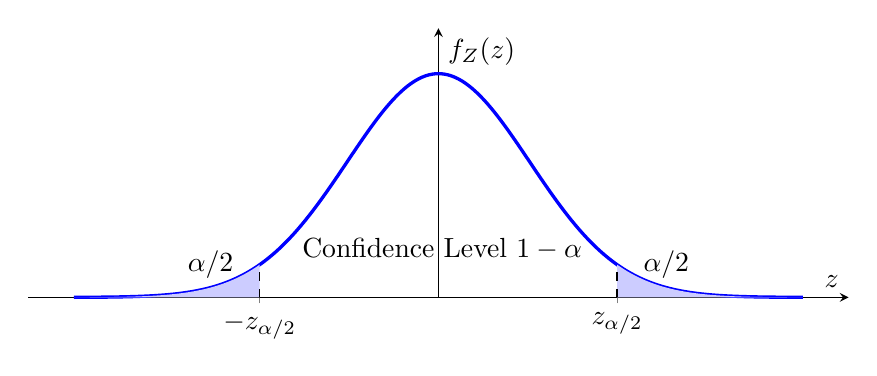
\begin{tikzpicture}
	\begin{axis}[
	no markers, domain=-4:4, samples=200,
	axis lines=center,
	%axis y line=none,
	xlabel={$z$}, ylabel={$f_Z(z)$},
	ymin=0, ymax=0.48,
	xmin=-4.5, xmax=4.5,
	height=5cm, width=12cm,
	xtick={-1.96,0,1.96},
	xticklabels={\(-z_{\alpha/2}\), 0, \(z_{\alpha/2}\)},
	ytick=\empty,
	clip=false
	]
	% PDF curve of standard normal
	\addplot [very thick, blue] {1/sqrt(2*pi)*exp(-x^2/2)};

	% Shade the confidence interval region [-z_alpha/2, z_alpha/2]
	\addplot [
	domain=-4:-1.96,
	draw=none,
	fill=blue!20,
	samples=100
	]
	{1/sqrt(2*pi)*exp(-x^2/2)} \closedcycle;

	\addplot [
	domain=1.96:4,
	draw=none,
	fill=blue!20,
	samples=100
	]
	{1/sqrt(2*pi)*exp(-x^2/2)} \closedcycle;

	% Vertical dashed lines at -z_alpha/2 and z_alpha/2
	\draw[dashed] (axis cs:-1.96,0) -- (axis cs:-1.96,{1/sqrt(2*pi)*exp(-1.96^2/2)});
	\draw[dashed] (axis cs:1.96,0) -- (axis cs:1.96,{1/sqrt(2*pi)*exp(-1.96^2/2)});

	% Labels
	\node[below] at (axis cs:-2.5,0.1) { ${\alpha/2}$};
	\node[below] at (axis cs:2.5,0.1) { ${\alpha/2}$};
	\node[above, black] at (axis cs:0.04,0.05) { Confidence Level \(1-\alpha\)};
	\end{axis}
	\end{tikzpicture}
\end{center}


Thus,
\[
P\left(-z_{\alpha/2} \leq Z \leq z_{\alpha/2}\right) = 1 - \alpha
\]
which translates to
\[
P\left(\overline{X} - z_{\alpha/2} \frac{\sigma}{\sqrt{n}} \leq \mu \leq \overline{X} + z_{\alpha/2} \frac{\sigma}{\sqrt{n}}\right) = 1 - \alpha
\]

Therefore, the $100(1-\alpha)\%$ confidence interval for $\mu$ is
\begin{textbox}
\[
\left[\overline{X} - z_{\alpha/2} \frac{\sigma}{\sqrt{n}}, \quad \overline{X} + z_{\alpha/2} \frac{\sigma}{\sqrt{n}} \right]
\]
\end{textbox}

\begin{itemize}
	\item For a 95\% confidence level, $1-\alpha = 0.95$. From table $z_{\alpha/2} = z_{0.025}= 1.96$.
	\item For a 99\% confidence level, $1-\alpha = 0.99$. From table $z_{\alpha/2} = z_{0.005} = 2.576$.
\end{itemize}


\textbf{Example}: Suppose the lifetimes of a certain type of battery are normally distributed with unknown mean $\mu$ and known standard deviation $\sigma = 10$ hours. A random sample of $n = 25$ batteries yields a sample mean of $\overline{X} = 100$ hours. Construct a 95\% confidence interval for the population mean lifetime.


\begin{itemize}
	\item Given: $\sigma = 10$, $n = 25$, $\overline{X} = 100$, and confidence level = 95\%
	\item For 95\% confidence, $z_{\alpha/2}= z_{0.025} = 1.96$
\end{itemize}

Compute the standard error:
\[
\frac{\sigma}{\sqrt{n}} = \frac{10}{\sqrt{25}} = \frac{10}{5} = 2
\]

Compute the margin of error:
\[
z_{\alpha/2} \cdot \frac{\sigma}{\sqrt{n}} = 1.96 \times 2 = 3.92
\]

Construct the confidence interval:
\[
\left[100 - 3.92, \quad 100 + 3.92\right] = [96.08,\ 103.92]
\]

We are 95\% confident that the true mean lifetime $\mu$ of the batteries lies between 96.08 and 103.92 hours.

\subsection{Population Variance Unknown}

Let $X_1, X_2, \dots, X_n$ be a random sample from a normal distribution $N(\mu, \sigma^2)$, where both $\mu$ and $\sigma^2$ are unknown. Let $\overline{X}$ be the sample mean and $S^2$ be sample variance.

The pivotal quantity
\[
T = \frac{\overline{X} - \mu}{S / \sqrt{n}}
\]
follows a Student's $t$-distribution with $\nu = n - 1$ degrees of freedom:
\[
T \sim t_{n-1}
\]
Let $t_{\alpha/2}, n-1$ be the critical value of the t-distribution such that $P(t > t_{\alpha/2, n-1})=\alpha/2$. Hence, we can write
\[
P\left(-t_{\alpha/2, n-1} \leq T \leq t_{\alpha/2, n-1}\right) = 1 - \alpha
\]
which implies
\[
P\left(\overline{X} - t_{\alpha/2, n-1} \frac{S}{\sqrt{n}} \leq \mu \leq \overline{X} + t_{\alpha/2, n-1} \frac{S}{\sqrt{n}}\right) = 1 - \alpha
\]

Therefore, the $100(1-\alpha)\%$ confidence interval for $\mu$ is
\begin{textbox}
\[
\left[\overline{X} - t_{\alpha/2, n-1} \frac{S}{\sqrt{n}}, \quad \overline{X} + t_{\alpha/2, n-1} \frac{S}{\sqrt{n}} \right]
\]
\end{textbox}


\section{Confidence Interval for the Variance in a Normal Population}

Consider a random sample $X_1, X_2, \dots, X_n$ from a normal distribution $N(\mu, \sigma^2)$ with unknown variance $\sigma^2$. Let $S^2$ be sample variance.

The pivotal quantity
\[
\chi^2 = \frac{(n-1) S^2}{\sigma^2}
\]
follows a chi-square distribution with $\nu = n-1$ degrees of freedom:
\[
\chi^2 \sim \chi^2_{n-1}
\]

We now need to find the critical values $L$ and $U$ such that
$$P\left(L \leq \frac{(n-1) S^2}{\sigma^2} \leq U\right) = 1 - \alpha$$

\begin{figure}[H]
\begin{center}
	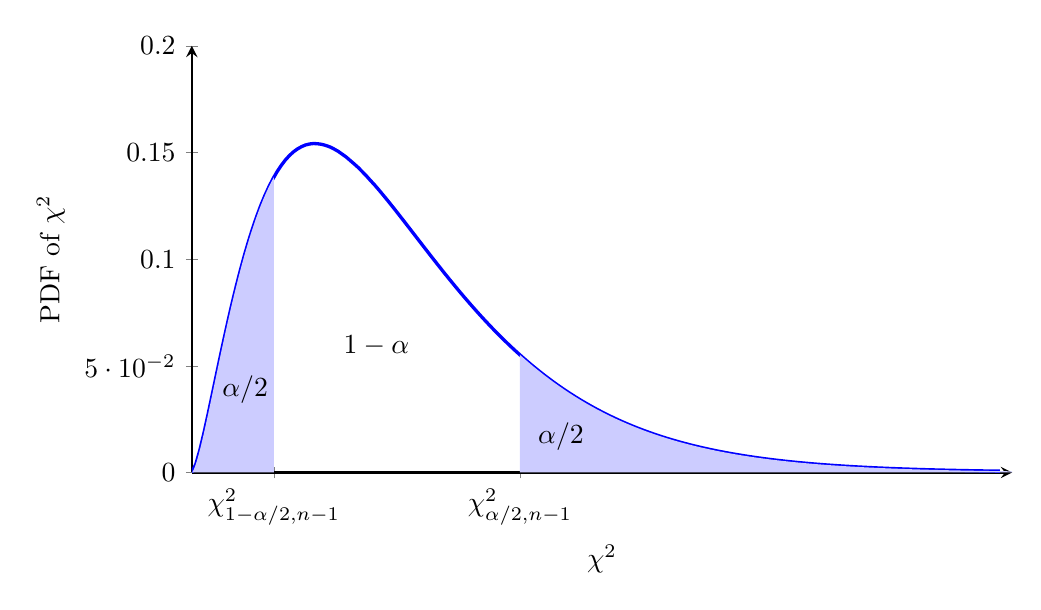
\begin{tikzpicture}
	\begin{axis}[
	width=12cm, height=7cm,
	domain=0:19.7, samples=200,
	axis lines=left,
	xlabel={$\chi^2$},
	ylabel={PDF of $\chi^2$},
	ymin=0, ymax=0.2,
	xmin=0, xmax=20,
	xtick={2,8},
	xticklabels={\(\chi_{1-\alpha/2, n-1}^2\), \(\chi_{\alpha/2, n-1}^2\)},
	% title={\small Chi-Squared Distributions for Different Degrees of Freedom},
	% grid=major,
	thick,
	]

	% ν = 5: f(x) = (1 / (2^{5/2} * Γ(5/2))) * x^{3/2} * exp(-x/2)
	% Γ(5/2) = 1.3293..., 2^{5/2} = 5.6568...
	% Constant = 1 / (5.6568 * 1.3293) ≈ 0.133
	\addplot [blue, very thick,] {0.133 * x^(1.5) * exp(-x/2)};

	% Shade the confidence interval region [-z_alpha/2, z_alpha/2]
	\addplot [
	domain=0:2,
	draw=none,
	fill=blue!20,
	samples=100
	]
	{0.133 * x^(1.5) * exp(-x/2)} \closedcycle;

	\addplot [
	domain=8:20,
	draw=none,
	fill=blue!20,
	samples=100
	]
	{0.133 * x^(1.5) * exp(-x/2)} \closedcycle;

	% Labels
	\node[below] at (axis cs:1.3,0.05) { ${\alpha/2}$};
	\node[below] at (axis cs:9,0.028) { ${\alpha/2}$};
	\node[above, black] at (axis cs:4.5,0.05) { \(1-\alpha\)};

	\end{axis}
	\end{tikzpicture}
	\caption{\textit{Confidence interval for $\chi^2$ distribution}.}
\end{center}
\end{figure}


We take areas to the left of $L$ and to the right of $R$ to be equal to $\alpha/2$ i.e.

$$L = \chi_{1-\alpha/2, n-1}^2, \quad R = \chi_{\alpha/2, n-1}^2$$

Thus,
\[
P\left(\chi^2_{1-\alpha/2, n-1} \leq \frac{(n-1) S^2}{\sigma^2} \leq \chi^2_{\alpha/2, n-1}\right) = 1 - \alpha
\]

Rearranging to solve for $\sigma^2$, we get
\[
P\left(\frac{(n-1) S^2}{\chi^2_{\alpha/2, n-1}} \leq \sigma^2 \leq \frac{(n-1) S^2}{\chi^2_{1-\alpha/2, n-1}}\right) = 1 - \alpha
\]

Therefore, the $100(1-\alpha)\%$ confidence interval for $\sigma^2$ is
\begin{textbox}
\[
\left[\frac{(n-1) S^2}{\chi^2_{1-\alpha/2, n-1}}, \quad \frac{(n-1) S^2}{\chi^2_{\alpha/2, n-1}} \right]
\]
\end{textbox}

\section{Confidence Interval for the Difference of Two Normally Distributed Population Means}

When comparing the means of two normally distributed populations, it is often of interest to estimate the difference between the population means, say \(\mu_1 - \mu_2\), using data from independent random samples from each population.

Let \(X_1, X_2, \dots, X_{n_1}\) be a random sample from population 1 with mean \(\mu_1\) and variance \(\sigma_1^2\), and \(Y_1, Y_2, \dots, Y_{n_2}\) be a random sample from population 2 with mean \(\mu_2\) and variance \(\sigma_2^2\). Let \(\overline{X}\) and \(\overline{Y}\) denote the respective sample means, and \(S_1^2\), \(S_2^2\) the respective sample variances.

We consider two cases:

\subsection{Population Variances Known}

Assume that \(\sigma_1^2\) and \(\sigma_2^2\) are known. Then the sampling distribution of \(\overline{X} - \overline{Y}\) is normal:
\[
\overline{X} - \overline{Y} \sim N\left(\mu_1 - \mu_2,\; \frac{\sigma_1^2}{n_1} + \frac{\sigma_2^2}{n_2} \right)
\]

Define the pivotal quantity:
\[
Z = \dfrac{(\overline{X} - \overline{Y}) - (\mu_1 - \mu_2)}{\sqrt{\dfrac{\sigma_1^2}{n_1} + \dfrac{\sigma_2^2}{n_2}}} \sim N(0,1)
\]

Then, a \(100(1 - \alpha)\%\) confidence interval for \(\mu_1 - \mu_2\) is given by:
\begin{textbox}
\[
\left[
(\overline{X} - \overline{Y}) - z_{\alpha/2} \sqrt{\frac{\sigma_1^2}{n_1} + \frac{\sigma_2^2}{n_2}}, \;
(\overline{X} - \overline{Y}) + z_{\alpha/2} \sqrt{\frac{\sigma_1^2}{n_1} + \frac{\sigma_2^2}{n_2}}
\right]
\]
\end{textbox}

\subsection{Population Variances Unknown}

Assume the populations are normally distributed but \(\sigma_1^2\) and \(\sigma_2^2\) are unknown. The confidence interval depends on whether variances can be assumed equal.

\begin{enumerate}[label=(\roman*)]
	\item \textbf{Equal but Unknown Variances:}

Assume \(\sigma_1^2 = \sigma_2^2 = \sigma^2\), and estimate with pooled variance:
\[
S_p^2 = \frac{(n_1 - 1)S_1^2 + (n_2 - 1)S_2^2}{n_1 + n_2 - 2}
\]

Then, the pivotal quantity
\[
T = \frac{(\overline{X} - \overline{Y}) - (\mu_1 - \mu_2)}{S_p \sqrt{\dfrac{1}{n_1} + \dfrac{1}{n_2}}} \sim t_{n_1 + n_2 - 2}
\]

Thus, the \(100(1 - \alpha)\%\) confidence limits is:
\begin{textbox}
\[
(\overline{X} - \overline{Y}) \pm t_{\alpha/2, \, n_1 + n_2 - 2} \cdot S_p \sqrt{\frac{1}{n_1} + \frac{1}{n_2}}
\]
\end{textbox}

\item \textbf{Unequal and Unknown Variances (Welch's Approximation):}

If equal variance cannot be assumed, use:
\[
T = \dfrac{(\overline{X} - \overline{Y}) - (\mu_1 - \mu_2)}{\sqrt{\dfrac{S_1^2}{n_1} + \dfrac{S_2^2}{n_2}}}
\]

This approximately follows a \(t\)-distribution with $\nu$ degrees of freedom, where:
\[
\nu \approx \dfrac{\left( \dfrac{S_1^2}{n_1} + \dfrac{S_2^2}{n_2} \right)^2}{\dfrac{1}{n_1 - 1}\left(\dfrac{S_1^2}{n_1} \right)^2 + \dfrac{1}{n_2 - 1}\left( \dfrac{S_2^2}{n_2}\right)^2}
\]

Then, the approximate \(100(1 - \alpha)\%\) confidence interval for \(\mu_1 - \mu_2\) is:
\begin{textbox}
\begin{align*}
\left[
(\overline{X} - \overline{Y}) - t_{\alpha/2, \nu} \cdot \sqrt{\frac{S_1^2}{n_1} + \frac{S_2^2}{n_2}}, \;
(\overline{X} - \overline{Y}) + t_{\alpha/2, \nu} \cdot \sqrt{\frac{S_1^2}{n_1} + \frac{S_2^2}{n_2}}
\right]
\end{align*}
\end{textbox}
\end{enumerate}


\section{Confidence Interval for the Ratio of Two Normally Distributed Population Variances}

Let \(X_1, X_2, \dots, X_{n_1}\) be a random sample from population 1 with mean \(\mu_1\) and variance \(\sigma_1^2\), and \(Y_1, Y_2, \dots, Y_{n_2}\) be a random sample from population 2 with mean \(\mu_2\) and variance \(\sigma_2^2\). Let \(S_1^2\), \(S_2^2\) denote the respective sample variances.

The pivotal quantity
\[
F \;=\;
\dfrac{S_1^2/\sigma_1^2}{S_2^2/\sigma_2^2} = \dfrac{S_1^2}{S_2^2}\cdot \dfrac{\sigma_2^2}{\sigma_1^2}
\]
follows an $F$–distribution with $(n_1-1,n_2-1)$ degrees of freedom.
\[
F \sim F_{\,n_1-1,\;n_2-1}
\]

Let $F_{1-\alpha/2;\,n_1-1,n_2-1}$ and $F_{\alpha/2;\,n_1-1,n_2-1}$ be the lower and upper $\alpha/2$–quantiles of this $F$–distribution:

\[
P\bigl(F_{1-\alpha/2;\,n_1-1,n_2-1}\le F\le F_{\alpha/2;\,n_1-1,n_2-1}\bigr) \;=\; 1-\alpha
\]

or,

\[
P\left( F_{1-\alpha/2;\,n_1-1,n_2-1}\le \dfrac{S_1^2}{S_2^2}\cdot \dfrac{\sigma_2^2}{\sigma_1^2} \leq F_{\alpha/2;\,n_1-1,n_2-1} \right) \;=\; 1-\alpha
\]

Rewriting in terms of $\sigma_1^2/\sigma_2^2$ gives

\[
P\left(
\frac{1}{F_{\alpha/2;\,n_1-1,n_2-1}}\frac{S_1^2}{S_2^2}
\;\le\;
\frac{\sigma_1^2}{\sigma_2^2}
\;\le\;
\frac{1}{F_{1-\alpha/2;\,n_1-1,n_2-1}}\frac{S_1^2}{S_2^2}
\right)
=1-\alpha
\]

Since for $ F $-distribution,
$$F_{1-\alpha/2;\,n_1-1,n_2-1} = \dfrac{1}{F_{\alpha/2;\,n_2-1,n_1-1}}$$

Therefore, a $100(1-\alpha)\%$ confidence interval for the ratio $\sigma_1^2/\sigma_2^2$ is

\begin{textbox}
	\[
	\left[
	\frac{1}{F_{\alpha/2;\,n_1-1,n_2-1}}\frac{S_1^2}{S_2^2}
	\;,\;
	{F_{\alpha/2;\,n_2-1,n_1-1}}\frac{S_1^2}{S_2^2}
	\right]
	\]
\end{textbox}


\section{Confidence Interval for a Population Proportion}

Let $X_1, X_2, \dots, X_n$ be a random sample from a Bernoulli population with unknown proportion parameter $p$. Define the sample proportion as
\[
\hat{p} = \frac{1}{n} \sum_{i=1}^{n} X_i = \frac{X}{n}
\]
where $X$ is the number of successes in the sample of size $n$.

For large $n$, the sampling distribution of $\hat{p}$ is approximately normal by the Central Limit Theorem:
\[
\hat{p} \sim N\left(p, \frac{p(1 - p)}{n}\right)
\]

Since $p$ is unknown, we approximate the standard deviation using $\hat{p}$, leading to the following pivotal quantity:
\[
Z = \frac{\hat{p} - p}{\sqrt{\dfrac{\hat{p}(1 - \hat{p})}{n}}}
\]

For sufficiently large $n$, $Z$ approximately follows the standard normal distribution:
\[
Z \sim N(0, 1)
\]
This approximation is generally considered valid when both \( n\hat{p} \geq 5 \) and \( n(1-\hat{p}) \geq 5 \).

Let $z_{\alpha/2}$ be the critical value from the standard normal distribution such that
\[
P(Z > z_{\alpha/2}) = \frac{\alpha}{2}
\]

Then,
\[
P\left(-z_{\alpha/2} \leq Z \leq z_{\alpha/2}\right) = 1 - \alpha
\]

This implies
\[
P\left(\hat{p} - z_{\alpha/2} \sqrt{\frac{\hat{p}(1 - \hat{p})}{n}} \leq p \leq \hat{p} + z_{\alpha/2} \sqrt{\frac{\hat{p}(1 - \hat{p})}{n}}\right) = 1 - \alpha
\]

Therefore, the $100(1 - \alpha)\%$ confidence interval for the population proportion $p$ is
\begin{textbox}
\[
\left[ \hat{p} - z_{\alpha/2} \sqrt{\frac{\hat{p}(1 - \hat{p})}{n}}, \quad \hat{p} + z_{\alpha/2} \sqrt{\frac{\hat{p}(1 - \hat{p})}{n}} \right]
\]
\end{textbox}

\bigskip

\textbf{Example}: A political poll surveys $n = 400$ registered voters to estimate the proportion who support Proposition~X. Out of the 400 respondents, $X = 180$ say they support the measure. Construct a 95\% confidence interval for the true support proportion $p$.

\begin{itemize}
	\item Sample size: $n = 400$
	\item Number of successes: $X = 180$
	\item Sample proportion:
	\[
	\hat{p} \;=\; \frac{X}{n} \;=\; \frac{180}{400} \;=\; 0.45
	\]
	\item Check normal approximation conditions:
	\[
	n\hat{p} = 400 \times 0.45 = 180 \;\ge 5,
	\quad
	n(1 - \hat{p}) = 400 \times 0.55 = 220 \;\ge 5.
	\]
	\item For 95\% confidence, $z_{\alpha/2} = z_{0.025} = 1.96$.
\end{itemize}

Compute the margin of error:
\[
z_{\alpha/2} \times \sqrt{\frac{\hat{p}(1 - \hat{p})}{n}}
= 1.96 \times \sqrt{\frac{0.45 \times 0.55}{400}}
\approx 1.96 \times 0.0249
\approx 0.0488
\]

Thus the 95\% confidence interval for $p$ is
\[
\bigl[\,0.45 - 0.0488,\;0.45 + 0.0488\bigr]
\;=\;
[\,0.4012,\;0.4988\,]
\]

We are 95\% confident that the true proportion of all registered voters who support Proposition~X lies between 40.12\% and 49.88\%.

\section{Determination of Sample Size}

Sample size determination is a fundamental aspect of planning any statistical study. If the sample is too small, the results may not be trustworthy. But if the sample is too large, it can waste time, money, and effort. The goal is to find a sample size that is just right: big enough to give accurate and useful results, but not bigger than necessary. There is no universal ideal sample size for all problems. The required sample size depends on:
\begin{itemize}
	\item The \textbf{parameter} being estimated,
	\item A specified \textbf{margin of error (E)},
	\item A desired \textbf{confidence level} (commonly 90\%, 95\%, or 99\%).
\end{itemize}

\subsection{Determining Sample Size for Estimating a Population Mean}

Let \(\mu\) denote the population mean and \(\sigma\) the population standard deviation (assumed known). To estimate \(\mu\) within a margin of error \(E\) at confidence level \(1 - \alpha\), the sample size \(n\) must satisfy:

\[
z_{\alpha/2} \cdot \frac{\sigma}{\sqrt{n}} \leq E
\]

Solving for \(n\):

\[
n \geq \left( \frac{z_{\alpha/2} \cdot \sigma}{E} \right)^2
\]

\textbf{Example:} A researcher wants to estimate the average height of adult males in a city with a 95\% confidence level and a margin of error of 2 cm. Suppose previous studies suggest \(\sigma = 7\) cm.

\begin{align*}
z_{\alpha/2} &= z_{0.025} = 1.96 \\
n &\geq \left( \frac{1.96 \cdot 7}{2} \right)^2 = \left( \frac{13.72}{2} \right)^2 = (6.86)^2 = 47.06
\end{align*}

Thus, a sample size of at least 48 individuals is needed.

\subsection{Determining Sample Size for Estimating a Population Proportion}

Suppose the goal is to estimate a population proportion \(p\). The margin of error in this case must satisfy:

\[
z_{\alpha/2} \cdot \sqrt{ \frac{p(1 - p)}{n} } \leq E
\]

Solving for \(n\):

\[
n \geq \left( \frac{z_{\alpha/2}}{E} \right)^2 \cdot p(1 - p)
\]

If the value of $p$ is known roughly in the neighbourhood of a value $p^*$, then $n$ can be determined as:
\[
n \geq \left( \frac{z_{\alpha/2}}{E} \right)^2 \cdot p^*(1 - p^*)
\]

Without prior knowledge of $p$, $p(1-p)$ can be replaced by its maximum possible value\footnote{To calculate the maximum value of $f=p(1-p) = p-p^2$, we need to differentiate it w.r.t. $p$ and set it to zero.
	$$\dfrac{df}{dp} = 1-2p = 0 \quad \Rightarrow p =\dfrac{1}{2}$$
$$\dfrac{d^2f}{dp^2}  = -2$$
The double derivative is negtive indicating $f$ is maximum at $p=\dfrac{1}{2}$.

\noindent The maximum value of $f$ is
$$f_{max} = \dfrac{1}{2}\left(1-\dfrac{1}{2}  \right) = \dfrac{1}{4}$$

} $\dfrac{1}{4}$ corresponding to $p=\dfrac{1}{2}$ and $n$ is determined from the relation:
\[
n \geq \dfrac{1}{4}\left( \frac{z_{\alpha/2}}{E} \right)^2
\]
\textbf{Example:} A political analyst wants to estimate the proportion of voters who support a candidate with 95\% confidence and a margin of error of 5\%. If no prior estimate for \(p\) is available, the conservative choice is \(p = 0.5\):

\begin{align*}
z_{\alpha/2} &= z_{0.025} = 1.96, \quad E = 0.05, \quad p = 0.5 \\
n &\geq \left( \frac{1.96}{0.05} \right)^2 \times 0.5 \times 0.5 = 1536.64 \times 0.25 = 384.16
\end{align*}

Thus, a sample size of at least 385 respondents is needed.

\subsection{Finite Population Correction (FPC)}

When sampling without replacement from a finite population of size \(N\), and the sample size \(n\) exceeds 5\% of the population (\(n > 0.05N\)), the effective sample size should be adjusted using the finite population correction (FPC):

\[
n_{\text{adj}} = \dfrac{n_0}{1 + \dfrac{n_0 - 1}{N}}
\]

where \(n_0\) is the sample size calculated assuming an infinite population.

\medskip

\noindent {To prove this formula let us rewrite the formula for the variance of the sample mean:}
\begin{itemize}
	\item {Finite population (without replacement):}
	\[
	\mathrm{Var}(\overline{X}) = \frac{\sigma^2}{n} \times \frac{N - n}{N - 1}
	\]
	\item {Infinite population (or with replacement):}
	\[
	\mathrm{Var}(\overline{X}) = \frac{\sigma^2}{n}
	\]
\end{itemize}

\medskip

To achieve the same precision (equal variances), set
\[
\frac{\sigma^2}{n_0} = \frac{\sigma^2}{n_{\text{adj}}} \times \frac{N - n_{\text{adj}}}{N - 1}
\]
where $n_0$ is the sample size required to achieve the variance for the infinite population and $n_{\text{adj}}$ is the sample size required to achieve the variance for the finite population.

Cancel \(\sigma^2\) and rearrange:
\begin{align*}
&\frac{1}{n_0} = \frac{1}{n_{\text{adj}}} \times \frac{N - n_{\text{adj}}}{N - 1} \\[6pt]
\Rightarrow \quad &n_{\text{adj}} \cdot \frac{N - 1}{n_0} = N - n_{\text{adj}}\\
\Rightarrow \quad &n_{\text{adj}} \left( 1 + \frac{N - 1}{n_0} \right) = N\\
\Rightarrow \quad &n_{\text{adj}} (n_0 + N - 1) = N n_0
\end{align*}

Hence, the adjusted sample size is
\[
	n_{\text{adj}} = \dfrac{N n_0}{n_0 + N - 1} = \dfrac{n_0}{1 + \dfrac{n_0 - 1}{N}}
\]



\textbf{Example:} From the earlier example, if the population consists of only 2,000 individuals:

\[
n_{\text{adj}} = \frac{384.16}{1 + \frac{384.16 - 1}{2000}} = \frac{384.16}{1 + 0.1916} = \frac{384.16}{1.1916} \approx 322.4
\]

Thus, only about 323 individuals are needed when the population is finite.

\section{Frequentist vs Bayesian Approaches of Statistical Inference}

The foundations of statistical inference are built on two major schools of thought: the frequentist and the Bayesian.

\begin{enumerate}
\item The \textbf{frequentist approach}, formalized in the early 20th century by statisticians like Ronald Fisher, Jerzy Neyman, and Egon Pearson, views parameters such as population means as fixed but unknown constants. In this framework, the probability is interpreted as the long-run frequency of events, and statistical inference is based on the behavior of data across repeated random samples.

\item In contrast, the \textbf{Bayesian approach}—rooted in the 18th-century work of Thomas Bayes but revived and expanded in modern times—treats unknown parameters as random variables with probability distributions that reflect prior beliefs. These beliefs are updated using Bayes’ theorem after observing data.
\end{enumerate}

The key distinction lies in interpretation: frequentists quantify uncertainty through the sampling distribution of estimators, while Bayesians express uncertainty directly about parameters using probability based on both data and prior information.

To illustrate the fundamental difference between the frequentist and Bayesian approaches we consider an example where we collect the heights (in cm) of 5 randomly selected adult men from a town:
\[
170,\quad 172,\quad 168,\quad 174,\quad 176
\]
The sample mean is:
\[
\bar{x} = \frac{170 + 172 + 168 + 174 + 176}{5} = 172
\]
We assume that the population standard deviation is known and equal to $\sigma = 4$ cm.

\vspace{1em}

\subsection{Frequentist Approach}

The frequentist treats the true mean $\mu$ as a fixed but unknown constant. The sample mean $\overline{x}$ is used as a point estimator for $\mu$. The goal is to make inference based on the behavior of $\overline{x}$ under repeated sampling.

\subsubsection*{Confidence Interval}

A 95\% confidence interval for the population mean $\mu$ is given by:
\[
\overline{x} \pm z_{\alpha/2} \cdot \dfrac{\sigma}{\sqrt{n}}
\]
Substituting values:
\[
172 \pm 1.96 \cdot \dfrac{4}{\sqrt{5}} \approx 172 \pm 3.51
\]
So the 95\% confidence interval is:
\[
[168.49,\; 175.51]
\]

\subsubsection*{Interpretation (Frequentist):}

If this sampling process were repeated many times, approximately 95\% of the confidence intervals constructed this way would contain the true population mean $\mu$. Note that in this view, $\mu$ is fixed and not random — the randomness lies in the interval.

\vspace{1em}

\subsection{Bayesian Approach}

The Bayesian treats the true mean $\mu$ as a random variable and assigns a prior distribution to reflect belief about $\mu$ before seeing data. This prior is then updated using Bayes’ theorem to obtain a posterior distribution after observing the data.

\subsubsection*{Prior Distribution}

Suppose we believe, before observing the data, that the average male height is centered around 170 cm, but we are not very confident. We use a normal prior:
\[
\mu \sim \mathcal{N}(170,\; 5^2)
\]

\subsubsection*{Posterior Distribution}

Given the normal prior and normal likelihood (due to known $\sigma$), the posterior distribution for $\mu$ is also normal:
\[
\mu \mid \text{data} \sim \mathcal{N}(\mu_{\text{post}},\; \sigma^2_{\text{post}})
\]
where
\[
\mu_{\text{post}} = \dfrac{\dfrac{170}{25} + \dfrac{172}{(4^2/5)}}{\dfrac{1}{25} + \dfrac{1}{(4^2/5)}} \approx 171.4, \qquad
\sigma_{\text{post}} \approx 1.6
\]

\subsubsection*{Credible Interval}

A 95\% credible interval is:
\[
\mu_{\text{post}} \pm 1.96 \cdot \sigma_{\text{post}} \approx 171.4 \pm 3.14 = [168.26,\; 174.54]
\]

\subsubsection*{Interpretation (Bayesian):}

Given the prior belief and the observed data, there is a 95\% probability that the true mean $\mu$ lies within the interval.

\vspace{1em}

\subsection{Summary of Differences}

\begin{table}[H]
\centering
\begin{tabular}{p{3.5cm}|p{4.2cm}|p{4.2cm}}
\toprule
\textbf{Aspect} & \textbf{Frequentist Approach} & \textbf{Bayesian Approach} \\
\midrule
Nature of $\mu$ & Fixed but unknown & Random variable with prior \\
\midrule
Use of prior knowledge & Not used & Incorporated through prior \\
\midrule
Interval interpretation & Probability attached to the confidence interval, not parameter & Probability applies to the parameter \\
\bottomrule
\end{tabular}
\caption{\textit{Comparison between frequentist and Bayesian interpretations.}}
\end{table}



% \begin{sidewaystable}[htbp]
% 	\centering
% 	\rotatebox{180}{%
% 		\begin{minipage}{\textheight}
% 			\centering
% 			\caption{Important Confidence Interval Formulas}
% 			\label{tab:ci_180_rotated}
% 			\begin{tabular}{@{}lll@{}}
% 				\toprule
% 				\textbf{Parameter} & \textbf{Assumptions} & \textbf{Confidence Interval Formula} \\ \midrule

% 				Population mean $\mu$ (known $\sigma$) &
% 				Normal population or large $n$ (CLT) &
% 				$\displaystyle \overline{X} \pm z_{\alpha/2} \cdot \frac{\sigma}{\sqrt{n}}$ \\[10pt]

% 				Population mean $\mu$ (unknown $\sigma$) &
% 				Normal population &
% 				$\displaystyle \overline{X} \pm t_{\alpha/2,\,n-1} \cdot \frac{s}{\sqrt{n}}$ \\[10pt]

% 				Difference of means $\mu_1 - \mu_2$ (equal variances) &
% 				Normal populations, independent samples &
% 				$\displaystyle (\overline{X}_1 - \overline{X}_2) \pm t_{\alpha/2,\,n_1+n_2-2} \cdot s_p \sqrt{\frac{1}{n_1} + \frac{1}{n_2}}$ \\
% 				& & where $\displaystyle s_p^2 = \frac{(n_1-1)s_1^2 + (n_2-1)s_2^2}{n_1 + n_2 - 2}$ \\[10pt]

% 				Proportion $p$ &
% 				Large $n$, with $np \ge 5$, $n(1-p) \ge 5$ &
% 				$\displaystyle \hat{p} \pm z_{\alpha/2} \cdot \sqrt{\frac{\hat{p}(1 - \hat{p})}{n}}$ \\[10pt]

% 				Difference of proportions $p_1 - p_2$ &
% 				Large $n_1, n_2$ &
% 				$\displaystyle (\hat{p}_1 - \hat{p}_2) \pm z_{\alpha/2} \cdot \sqrt{ \frac{\hat{p}_1(1 - \hat{p}_1)}{n_1} + \frac{\hat{p}_2(1 - \hat{p}_2)}{n_2} }$ \\[10pt]

% 				Population variance $\sigma^2$ &
% 				Normal population &
% 				$\displaystyle \left( \frac{(n-1)s^2}{\chi^2_{1-\alpha/2}}, \frac{(n-1)s^2}{\chi^2_{\alpha/2}} \right)$ \\[10pt]

% 				Ratio of variances $\frac{\sigma_1^2}{\sigma_2^2}$ &
% 				Normal, independent samples &
% 				$\displaystyle \left( \dfrac{s_1^2 / s_2^2}{F_{1-\alpha/2}}, \dfrac{s_1^2 / s_2^2}{F_{\alpha/2}} \right)$ \\

% 				\bottomrule
% 			\end{tabular}
% 		\end{minipage}
% 	}
% \end{sidewaystable}

\begin{sidewaystable}
	\centering
	\begin{tabular}{@{}lll@{}}
		\toprule
		\textbf{Parameter} & \textbf{Assumptions} & \textbf{Confidence Interval Formula} \\ \midrule

		Population mean $\mu$ (known $\sigma$) &
		Normal population or large $n$ (CLT) &
		$\displaystyle \overline{X} \pm z_{\alpha/2} \cdot \frac{\sigma}{\sqrt{n}}$ \\[10pt]

		Population mean $\mu$ (unknown $\sigma$) &
		Normal population &
		$\displaystyle \overline{X} \pm t_{\alpha/2,\,n-1} \cdot \frac{s}{\sqrt{n}}$ \\[10pt]

		Difference of means $\mu_1 - \mu_2$ (equal variances) &
		Normal populations, independent samples &
		$\displaystyle (\overline{X}_1 - \overline{X}_2) \pm t_{\alpha/2,\,n_1+n_2-2} \cdot s_p \sqrt{\frac{1}{n_1} + \frac{1}{n_2}}$ \\
		& & where $\displaystyle s_p^2 = \frac{(n_1-1)s_1^2 + (n_2-1)s_2^2}{n_1 + n_2 - 2}$ \\[10pt]

		Proportion $p$ &
		Large $n$, with $np \ge 5$, $n(1-p) \ge 5$ &
		$\displaystyle \hat{p} \pm z_{\alpha/2} \cdot \sqrt{\frac{\hat{p}(1 - \hat{p})}{n}}$ \\[10pt]

		Difference of proportions $p_1 - p_2$ &
		Large $n_1, n_2$ &
		$\displaystyle (\hat{p}_1 - \hat{p}_2) \pm z_{\alpha/2} \cdot \sqrt{ \frac{\hat{p}_1(1 - \hat{p}_1)}{n_1} + \frac{\hat{p}_2(1 - \hat{p}_2)}{n_2} }$ \\[10pt]

		Population variance $\sigma^2$ &
		Normal population &
		$\displaystyle \left( \frac{(n-1)s^2}{\chi^2_{1-\alpha/2}}, \frac{(n-1)s^2}{\chi^2_{\alpha/2}} \right)$ \\[10pt]

		Ratio of variances $\dfrac{\sigma_1^2}{\sigma_2^2}$ &
		Normal, independent samples &
		$\displaystyle \left( \dfrac{s_1^2 / s_2^2}{F_{1-\alpha/2}}, \dfrac{s_1^2 / s_2^2}{F_{\alpha/2}} \right)$ \\

		\bottomrule
	\end{tabular}
    \caption{\textit{Important confidence interval formulas.}}
	\label{tab:ci_sideways}
\end{sidewaystable}


\chapter{Test of Hypothesis}
\section{What is Hypothesis Testing?}

There are many problems in which, rather than estimating the value of a parameter, we must decide whether a statement concerning a parameter is true or false. Statistically speaking, we test a hypothesis about a parameter.

% \begin{tcolorbox}[heading={Statistical Hypothesis}]
% A \textbf{statistical hypothesis} is a statement about the parameter of a population.
% \end{tcolorbox}

\begin{textbox}
A \textbf{statistical hypothesis} is a statement about the parameter of a population.
\end{textbox}

For example, a factory produces screws that are supposed to be 5 cm long. A quality inspector takes a sample of 50 screws and finds that the average length is 4.8 cm. Here, the hypothesis is the statement:

\begin{center}
``{The average length of the screws is 5 cm.}''
\end{center}

Based on the sample's average length, the inspector tests whether this difference is simply due to random variation or if the machine requires adjustment.

\begin{textbox}
\textbf{Hypothesis testing} is a formal procedure for testing a claim or hypothesis about a population parameter using sample data.
\end{textbox}
It helps us to determine whether the evidence in a sample supports a certain belief or hypothesis about the population.

\subsection{Null and Alternative Hypothesis}

The hypothesis that will actually be tested is called the \textbf{null hypothesis}, denoted by $H_0$. This is a particular claim about a population parameter. The null hypothesis is assumed to be true unless there is any strong evidence to the contrary.

The \textbf{alternative hypothesis}, denoted by $H_1$ or $H_a$, is a hypothesis that contradicts the null hypothesis. These two hypotheses are mutually exclusive and
exhaustive so that one is true to the exclusion of the
other. For the above example, we define the hypotheses as:

\begin{itemize}
    \item \textbf{Null Hypothesis ($H_0$):} The average length of screws is 5 cm.
    \item \textbf{Alternative Hypothesis ($H_1$ or $H_a$):} The average length is not 5 cm.
\end{itemize}

In simple expression we write:
    $$H_0: \mu = 5$$
    $$H_1 : \mu \neq 5$$

% The objective of hypothesis testing is to decide, based on
% sample information, if the alternative hypothesis is actually
% supported by the data.

The standard procedure is to assume that $H_0$ is true. The burden of proof is placed on those who believe in the alternative claim\footnote{A close analogy can be made to a criminal court trial, where the jury holds to the null hypothesis of ``Not guilty'' unless there is convincing evidence of guilt.  The purpose of the hearing is to establish the assertion that the accused is guilty rather than to prove that he or she is innocent.} (alternative hypothesis). This initially favored claim ($H_0$) will not be rejected in favor of the alternative claim ($H_1$ or $H_a$) unless the sample evidence provides significant support for the alternative claim. If the sample does not strongly contradict $H_0$, we will continue to believe in the plausibility of the null hypothesis.

\vspace{3mm}
\begin{center}
    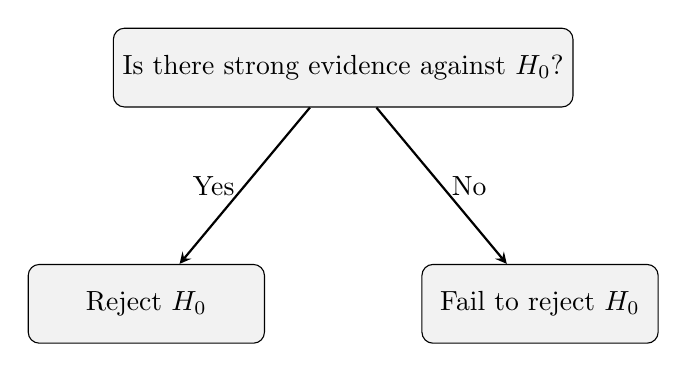
\begin{tikzpicture}[node distance=3cm]

% Nodes
% \node (start) [startstop] {Start Hypothesis Test};
\node (evidence) [startstop] {Is there strong evidence against $H_0$?};
\node (reject) [startstop, below of=evidence, xshift=-2.5cm] {Reject $H_0$};
\node (fail) [startstop, below of=evidence, xshift=2.5cm] {Fail to reject $H_0$};

% Arrows
% \draw [arrow] (start) -- (evidence);
\draw [arrow] (evidence) -- node[left] {Yes} (reject);
\draw [arrow] (evidence) -- node[right] {No} (fail);

\end{tikzpicture}
\end{center}

Statisticians avoid saying ``accept $H_0$'' because it wrongly implies that the null hypothesis has been proven true. When there is no strong evidence against $H_0$, we retain it—but this does not confirm its truth; instead, we say we ``fail to reject $H_0$''. On the other hand, when the evidence is strong, we confidently ``reject $H_0$''. Thus, rejecting $H_0$ is a \textbf{strong decision}, supported by sufficient evidence, while retaining $H_0$ is a \textbf{weak decision}, reflecting inconclusive results.

To test the hypothesis in the above example, we assume that the
standard deviation $\sigma = 0.3$ is known. Since the sample size is $n = 50$, the sampling distribution of the sample mean is approximately normal: \[
    \overline{X} \sim N\left( \mu, \frac{\sigma}{\sqrt{n}} \right)
    \]
    \text{or, } \[
    \overline{X} \sim N\left( 50, 0.042 \right)
    \]

\begin{figure}[h]
\begin{center}
	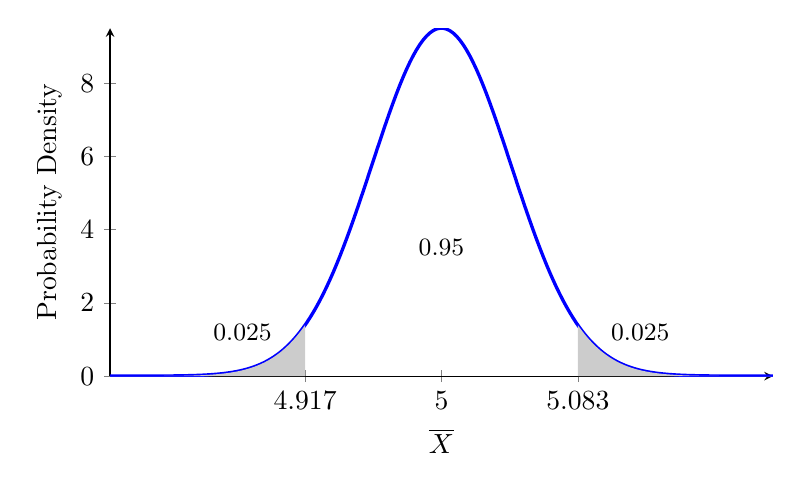
\begin{tikzpicture}
	\begin{axis}[
	domain=4.8:5.2, samples=200,
	xlabel={$\overline{X}$}, ylabel={Probability Density},
	axis lines=left,
	height=6cm, width=10cm,
	xtick={4.9177, 5, 5.0823},
	xticklabels={$4.917$, $5$, $5.083$}
	]

	% Plot the normal curve
	\addplot [very thick, blue] {1/(0.042*sqrt(2*pi)) * exp(-((x-5)^2)/(2*0.042^2))};

	% Shade the left tail
	\addplot [
	domain=4.8:4.9177,
	fill=gray!40,
	draw=none
	] {1/(0.042*sqrt(2*pi)) * exp(-((x-5)^2)/(2*0.042^2))} \closedcycle;

	% Shade the right tail
	\addplot [
	domain=5.0823:5.2,
	fill=gray!40,
	draw=none
	] {1/(0.042*sqrt(2*pi)) * exp(-((x-5)^2)/(2*0.042^2))} \closedcycle;

	% Add probability text
	\node at (axis cs:5,3.5) {\small 0.95};
	\node at (axis cs:4.88,1.2) {\small 0.025};
	\node at (axis cs:5.12,1.2) {\small 0.025};

	\end{axis}
	\end{tikzpicture}
\end{center}
\caption{\textit{Sampling distribution of sample mean for the screw length.}}
\label{fig:sampling_dist_screw_mean}
\end{figure}

% \begin{center}
% \begin{tikzpicture}
%   \begin{axis}[
%     domain=-3.5:3.5, samples=200,
%     xlabel={$\overline{X}$}, ylabel={Probability Density},
%     axis lines=left,
%     height=6cm, width=10cm,
%     xtick={-1.96, 0, 1.96},
%     xticklabels={$ \mu - z_{\alpha/2} $, $ \mu $, $ \mu + z_{\alpha/2} $},
%     enlargelimits=0.1
%   ]

%     % Plot the normal curve
%     \addplot [very thick, blue] {1/sqrt(2*pi) * exp(-x^2/2)};

%     % Shade the left tail
%     \addplot [
%       domain=-3.5:-1.96,
%       fill=gray!40,
%       draw=none
%     ] {1/sqrt(2*pi) * exp(-x^2/2)} \closedcycle;

%     % Shade the right tail
%     \addplot [
%       domain=1.96:3.5,
%       fill=gray!40,
%       draw=none
%     ] {1/sqrt(2*pi) * exp(-x^2/2)} \closedcycle;

%     % Add probability text
%     \node at (axis cs:0,0.25) {\small $1 - \alpha$};
%     \node at (axis cs:-2.6,0.05) {\small $\alpha/2$};
%     \node at (axis cs:2.6,0.05) {\small $\alpha/2$};

%   \end{axis}
% \end{tikzpicture}
% \end{center}


The distribution of $\overline{X}$ (sampling distribution) is shown in Figure \ref{fig:sampling_dist_screw_mean}. From the figure, we can see that there is a $95\%$ chance that the value of $\overline{X}$ measured from a random sample will lie in the region $4.917 \leq \overline{X} \leq 5.083$. However, the observed value is 4.8 cm, which falls well outside of this interval. The chance of obtaining such an extreme value when the true mean is actually 5 cm is less than $5\%$.

This provides strong statistical evidence against the null hypothesis. Therefore, we reject the null hypothesis $H_0: \mu = 5$ in favor of the alternative hypothesis $H_1: \mu \ne 5$. It suggests that the mean length of the screws is significantly different from 5 cm, and that the manufacturing process may need to be adjusted.


\begin{textbox}
The probability of the tails of the distribution, which determines the threshold for making a decision, is called the \textbf{level of significance}, denoted by $\alpha$.
\end{textbox}
In our example, we chose the level of significance $\alpha = 0.05$, which is equally split between the two tails of the distribution, allocating $0.025$ to each side.

\begin{textbox}
The range of values for which the null hypothesis is
rejected is called the \textbf{critical region}.
\end{textbox}

For the above example, the critical region is characterized by $\overline{X} < 4.917$ and $\overline{X} > 5.083$.

\subsection{One-Sided and Two-Sided Hypothesis Testing}

In hypothesis testing, the form of the alternative hypothesis determines whether the test is \textbf{one-sided} (one-tailed) or \textbf{two-sided} (two-tailed).

\begin{itemize}
    \item \textbf{Two-Sided Test:} Used when we are interested in detecting any difference from the null hypothesis value, whether it is an increase or a decrease. For example:
    \[
    H_0: \mu = 5 \quad \text{vs.} \quad H_1: \mu \ne 5
    \]
    This test considers deviations on both sides of the hypothesized mean as we saw in the previous example. The significance level $\alpha$ is split between the two tails of the sampling distribution.

    \item \textbf{One-Sided Test:} Used when we are only interested in deviations in one direction.
    \begin{itemize}
        \item To test if the mean is \emph{less than} 5:
        \[
        H_0: \mu = 5 \quad \text{vs.} \quad H_1: \mu < 5
        \]
        \item To test if the mean is \emph{greater than} 5:
        \[
        H_0: \mu = 5 \quad \text{vs.} \quad H_1: \mu > 5
        \]
    \end{itemize}
    In this case, the entire significance level $\alpha$ is placed in one tail of the distribution.
\end{itemize}

\noindent
The choice between one-sided and two-sided testing depends on the research question. If deviations in both directions are meaningful, a two-sided test is appropriate. If only an increase or a decrease is relevant, a one-sided test is more powerful.


% \section{Tests of Statistical Hypotheses}

% Let us take the same previous example where a factory claims that the average length of screws produced by a machine is 5 cm. To verify this claim, a quality inspector takes a random sample of 50 screws and finds that the average length is 4.8 cm. We want to test whether this observed difference is due to random sampling variation or if it indicates that the machine is no longer operating correctly.

% \begin{enumerate}
%     \item \textbf{State the Hypotheses:}
%     \begin{itemize}
%         \item Null Hypothesis ($H_0$): The true mean length is 5 cm. $$H_0: \mu = 5$$
%         \item Alternative Hypothesis ($H_1$): The true mean length is not 5 cm. $$H_1: \mu \ne 5$$
%     \end{itemize}

%     \item \textbf{Compute the Test Statistic} \\
%     The \textbf{test statistic} is a function of the sample data that will be used to make a decision about whether the null hypothesis should be rejected or not.

%     Assume that the population standard deviation is known to be $\sigma = 0.3$ cm. Since the sample size is $n = 50$, the sampling distribution of the sample mean is approximately normal:
%     \[
%     \overline{X} \sim N\left( \mu, \frac{\sigma}{\sqrt{n}} \right)
%     \]
%     This implies that
%     \[
%     Z = \dfrac{\overline{x} - \mu_0}{\dfrac{\sigma}{\sqrt{n}}}
%     \]
%     will follow a standard normal distribution, or Z distribution. The z-test statistic is:
%     \[
%     z = \frac{\overline{x} - \mu_0}{\frac{\sigma}{\sqrt{n}}} = \frac{4.8 - 5}{\frac{0.3}{\sqrt{50}}} \approx -4.72
%     \]

%     \item \textbf{Determine the Critical Region:}
%     For standard normal distribution, we know
%     \[
%     Prob\left[-z_{\frac{\alpha}{2}} < Z < z_{\frac{\alpha}{2}}\right] = 1-\alpha
%     \]
%     For $\alpha=0.05$, $z_{\frac{\alpha}{2}} = 1.96$, and therefore
%     \[
%     Prob\left[-1.96 < Z < 1.96\right] = 0.95
%     \]
%     The region outside
%     \[-1.96 < Z < 1.96\]
%     is called the critical region. The probability that the z-value will fall in the critical region is 0.05 and if the computed z-value falls in the critical region, we reject the null hypothesis. The computed z-value in this example is $-4.72$, which falls in the critical region ($z < -1.96$), we reject the null hypothesis.

%     \item \textbf{Conclusion} \\
%     We reject the null hypothesis $H_0$. There is strong statistical evidence that the true mean length of the screws is not 5 cm. This suggests the machine may be out of adjustment.
% \end{enumerate}

\section{Test Statistic}
\begin{textbox}
The \textbf{test statistic} is a function of the sample data that forms the basis for making the statistical decision to either reject or not reject the null hypothesis.
\end{textbox}

The main purpose of the test statistic is to provide a measure of how far the sample statistic (such as the sample mean) deviates from the hypothesized value under the null hypothesis. The further this value is from the hypothesized value, the stronger the evidence against the null hypothesis.

Depending on the type of hypothesis test being conducted, the test statistic can take various forms. For instance, a \textbf{$ z $-test statistic} is used to test hypotheses about a population mean when the population standard deviation ($\sigma$) is known and the sample size is large ($n > 30$). The $ z $-test compares the sample mean to the population mean, and the test statistic is given by:
    \[
    Z = \dfrac{\overline{X} - \mu_0}{{\sigma}/{\sqrt{n}}}
    \]
where $\overline{X}$ is the sample mean, $\mu_0$ is the population mean under the null hypothesis, $\sigma$ is the population standard deviation, and $n$ is the sample size. If the null hypothesis is true, $ \mathbb{E}(\overline{X}) = \mu_0 $, and it follows that the distribution of $ Z $ is the standard normal distribution i.e. $Z \sim \mathcal{N}(0,1)$.

For the example with a sample of 50 screws, where the sample mean is $\overline{X} = 4.8$ cm, the population mean under the null hypothesis is $\mu_0 = 5$ cm, and the population standard deviation is $\sigma = 0.3$ cm. The $ z $-test statistic is then calculated as follows:

\[
Z = \dfrac{\overline{X} - \mu}{{\sigma}/{\sqrt{n}}} = \frac{4.8 - 5}{{0.3}/{\sqrt{50}}} \approx -4.72
\]

Once the test statistic is calculated, it is compared with a \textbf{critical value} calculated from the relevant probability distribution of the test statistic under null hypothesis (e.g., the standard normal distribution). The critical value \(c\) is chosen so that
\[
P(\text{Test Statistic is more extreme than }c \mid H_0) = \alpha
\]
where \(\alpha\) is the level of significance.  Equivalently, the set of all values of the test statistic that lead to rejection of \(H_0\) is called the \textbf{critical region} or \textbf{rejection region}. Therefore

$$P(\text{Test statistic} \in \text{rejection region}\mid H_0) = \alpha$$

\begin{table}[H]
	\centering
	\begin{tabular}{@{}l|c|c@{}}
		\toprule
		\textbf{Test Type} & \textbf{Critical Value(s)} & \textbf{Rejection Region} \\
		\midrule
		Upper‐tailed \(z\)‑test & $ z_{\alpha} $ &
		\(\{Z>z_{\alpha}\}\) \\[6pt]
		Lower‐tailed \(z\)‑test &
		$ -z_{\alpha} $ &
		\(\{Z<-z_{\alpha}\}\) \\[6pt]
		Two‐tailed \(z\)‑test &
		$ \pm\,z_{\alpha/2} $&
		$\{|Z| > z_{\alpha/2}\}$ \\
		\bottomrule
	\end{tabular}
	\caption{\textit{Critical values and rejection regions for \(z\)-tests at significance level \(\alpha\)}.}
\end{table}


%For instance, in a two‐tailed test with \(\alpha = 0.05\), the critical values are \(\pm 1.96\).

 \begin{figure}[H]
 	\begin{center}
 		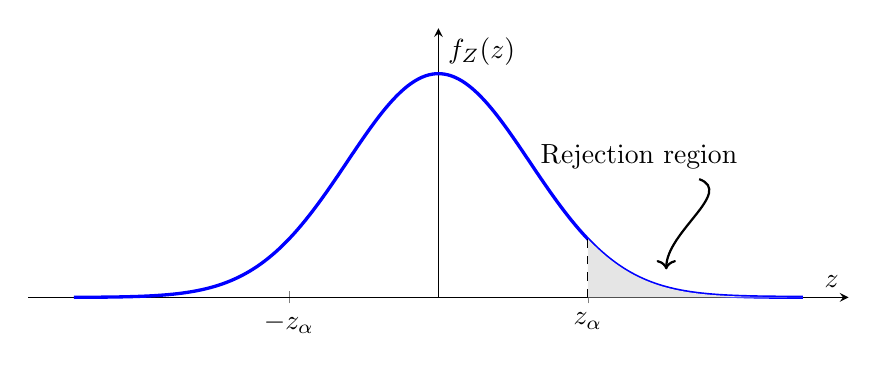
\begin{tikzpicture}
 		\begin{axis}[
 		no markers, domain=-4:4, samples=200,
 		axis lines=center,
 		xlabel={$z$}, ylabel={$f_Z(z)$},
 		ymin=0, ymax=0.48,
 		xmin=-4.5, xmax=4.5,
 		height=5cm, width=12cm,
 		xtick={-1.64,0,1.64},
 		xticklabels={\(-z_{\alpha}\), 0, \(z_{\alpha}\)},
 		ytick=\empty,
 		clip=false
 		]
 		% PDF curve of standard normal
 		\addplot [very thick, blue] {1/sqrt(2*pi)*exp(-x^2/2)};

 		% Shade the critical regions (tails)
 		\addplot [
 		domain=1.64:4,
 		draw=none,
 		fill=gray!20,
 		samples=100
 		]
 		{1/sqrt(2*pi)*exp(-x^2/2)} \closedcycle;

 		% Vertical dashed lines
 		\draw[dashed] (axis cs:1.64,0) -- (axis cs:1.64,{1/sqrt(2*pi)*exp(-1.64^2/2)});

 		% Single label with two arrows
 		\node (label) at (axis cs:2.2,0.25) {{Rejection region}};
 		\draw[->, thick] (label) to[out=-20,in=90] (axis cs: 2.5,0.05);
 		\end{axis}
 		\end{tikzpicture}
 	\end{center}
 	\caption{\textit{Rejection region for upper‐tailed \(z\)-test.}}
 \end{figure}

 \begin{figure}[H]
	\begin{center}
		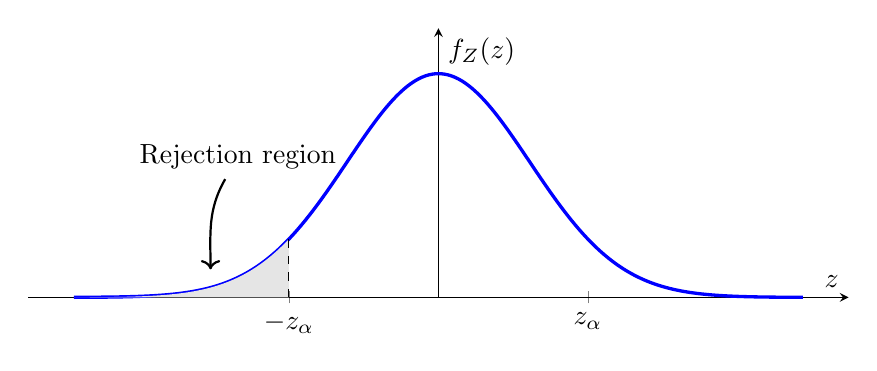
\begin{tikzpicture}
		\begin{axis}[
		no markers, domain=-4:4, samples=200,
		axis lines=center,
		xlabel={$z$}, ylabel={$f_Z(z)$},
		ymin=0, ymax=0.48,
		xmin=-4.5, xmax=4.5,
		height=5cm, width=12cm,
		xtick={-1.64,0,1.64},
		xticklabels={\(-z_{\alpha}\), 0, \(z_{\alpha}\)},
		ytick=\empty,
		clip=false
		]
		% PDF curve of standard normal
		\addplot [very thick, blue] {1/sqrt(2*pi)*exp(-x^2/2)};

		% Shade the critical regions (tails)
		\addplot [
		domain=-4:-1.64,
		draw=none,
		fill=gray!20,
		samples=100
		]
		{1/sqrt(2*pi)*exp(-x^2/2)} \closedcycle;

		% Vertical dashed lines
		\draw[dashed] (axis cs:-1.64,0) -- (axis cs:-1.64,{1/sqrt(2*pi)*exp(-1.64^2/2)});

		% Single label with two arrows
		\node (label) at (axis cs:-2.2,0.25) {{Rejection region}};
		\draw[->, thick] (label) to[out=-120,in=90] (axis cs: -2.5,0.05);
		\end{axis}
		\end{tikzpicture}
	\end{center}
	\caption{\textit{Rejection region for lower‐tailed \(z\)-test.}}
\end{figure}

\begin{figure}[H]
	\begin{center}
		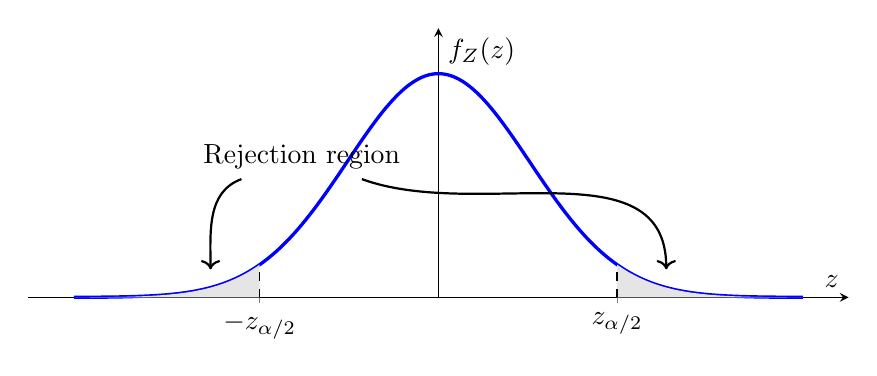
\begin{tikzpicture}
		\begin{axis}[
		no markers, domain=-4:4, samples=200,
		axis lines=center,
		xlabel={$z$}, ylabel={$f_Z(z)$},
		ymin=0, ymax=0.48,
		xmin=-4.5, xmax=4.5,
		height=5cm, width=12cm,
		xtick={-1.96,0,1.96},
		xticklabels={\(-z_{\alpha/2}\), 0, \(z_{\alpha/2}\)},
		ytick=\empty,
		clip=false
		]
		% PDF curve of standard normal
		\addplot [very thick, blue] {1/sqrt(2*pi)*exp(-x^2/2)};

		% Shade the critical regions (tails)
		\addplot [
		domain=-4:-1.96,
		draw=none,
		fill=gray!20,
		samples=100
		]
		{1/sqrt(2*pi)*exp(-x^2/2)} \closedcycle;

		\addplot [
		domain=1.96:4,
		draw=none,
		fill=gray!20,
		samples=100
		]
		{1/sqrt(2*pi)*exp(-x^2/2)} \closedcycle;

		% Vertical dashed lines at -z_alpha/2 and z_alpha/2
		\draw[dashed] (axis cs:-1.96,0) -- (axis cs:-1.96,{1/sqrt(2*pi)*exp(-1.96^2/2)});
		\draw[dashed] (axis cs:1.96,0) -- (axis cs:1.96,{1/sqrt(2*pi)*exp(-1.96^2/2)});

		% Single label with two arrows
		\node (label) at (axis cs:-1.5,0.25) {{Rejection region}};
		\draw[->, thick] (label) to[out=200,in=90] (axis cs:-2.5,0.05);
		\draw[->, thick] (label) to[out=-20,in=90] (axis cs: 2.5,0.05);
		\end{axis}
		\end{tikzpicture}
	\end{center}
	\caption{\textit{Rejection region for two‐tailed \(z\)-test.}}
\end{figure}



\noindent {Now we set the decision rule:}
\begin{itemize}
	\item If the observed test statistic \(z_{\rm obs}\) lies in the rejection region, then we reject \(H_0\).
	\item Otherwise, we fail to reject \(H_0\).
\end{itemize}

In our example, the computed \(z\)-value is \(-4.72\), which lies in the left‐hand critical region \(\{Z < z_{\alpha/2} = -1.96\}\) for the two-tailed test with $\alpha = 0.05$. Therefore, we reject the null hypothesis \(H_0\). In general, the larger the magnitude of the test statistic, the stronger the evidence against the null hypothesis.

\section{Parametric vs. Non‑Parametric Tests}

In statistical inference, tests are often classified according to the assumptions they make about the population distribution.  Two broad families are \textbf{parametric} and \textbf{non‑parametric} tests.
\begin{itemize}
\item \textbf{Parametric Tests}:
Parametric tests rely on specific assumptions about the form of the underlying population distribution, typically that it belongs to a known family (e.g.\ the normal distribution).  They are characterized by:


\item \textbf{Non‑Parametric Tests}:
Non‑parametric tests make \emph{fewer} assumptions about the population distribution.  They often use the ranking or signs of the data rather than their numerical values.  Key features include:
\end{itemize}

\begin{table}[H]
\centering
\begin{tabular}{p{2cm}|p{5cm}|p{5cm}}
\toprule
\textbf{Characteristic} & \textbf{Parametric Tests} & \textbf{Non‑Parametric Tests} \\
\midrule
Distribution assumption
  & Assume a known distribution (e.g.\ normal)
  & Do not assume a specific distribution \\
\midrule
Data usage
  & Use parameters like mean ($\mu$) and variance ($\sigma^2$)
  & Use ranks, signs, or counts instead of raw values \\
\midrule
Data scale
  & Require interval or ratio data
  & Work with ordinal or non‑normal interval/ratio data \\
\midrule
When to use
  & For well‑behaved numeric data meeting assumptions
  & When assumptions fail or data are ordinal \\
\midrule
Examples
  & $Z$-test, $t$‑test, ANOVA, Pearson’s correlation
  & Mann–Whitney $U$, Wilcoxon signed‑rank, chi‑square \\
\bottomrule
\end{tabular}
\caption{\textit{Comparison of Parametric and Non‑Parametric Tests}}
\end{table}

In this and the following chapters, we will focus on parametric tests. A dedicated chapter on non-parametric tests will be presented later.


\section{Type I and Type II Error}
This decision procedure can lead to either of two incorrect conclusions, known as Type I and Type II errors.

For example, suppose the true average length of the screws is indeed 5 cm. However, due to random variation in the sample, we might observe a test statistic that falls into the critical region. In this case, we would reject the null hypothesis $H_0$ in favor of the alternative $H_1$, even though $H_0$ is actually true. This mistake is called a \textbf{Type I error}. The probability of a Type I error is also called the \textbf{level of significance}, denoted by $\alpha$. It is usually set at $\alpha = 0.05$ or $\alpha = 0.01$.

\begin{textbox}
	\centering $P$(\text{Type I error})  = $P$(Rejecting $H_0$ $\mid$ $H_0$ is true) = $\alpha$
\end{textbox}

On the other hand, suppose the true average length of the screws has actually changed (for example, to 4.8 cm), but the observed sample does not provide enough evidence (such as 4.92 cm) to reject $H_0$. In this case, we fail to reject the null hypothesis, even though it is false. This mistake is called a \textbf{Type II error}. The probability of Type II error is denoted by $\beta$.

\begin{textbox}
	\centering $P$(\text{Type II error}) = $P$(Not rejecting $H_0$ $\mid$ $H_0$ is false) = $\beta$
\end{textbox}

\begin{table}[H]
	\centering
	\vspace{0.5em}
	\renewcommand{\arraystretch}{1.5}
	\begin{tabular}{l|c|c}

		& $H_0$ is True & $H_1$ is True \\
		\midrule
		Reject $H_0$        & \textbf{Type I Error} ($\alpha$) & Correct Decision \\
		Fail to Reject $H_0$ & Correct Decision        & \textbf{Type II Error} ($\beta$) \\
	\end{tabular}
\end{table}

\subsection{Tradeoff between Type I and Type II Errors}

These error probabilities are inherently related through the choice of the rejection region. Generally, reducing \(\alpha\) increases \(\beta\), and vice versa. This trade-off can be visualized by the overlapping distributions of the test statistic (sample mean in the picture) under \(H_0\) and \(H_1\) as shown in Figure~\ref{fig:type-i_and_type-ii}.

\begin{figure}[H]
	\begin{center}
		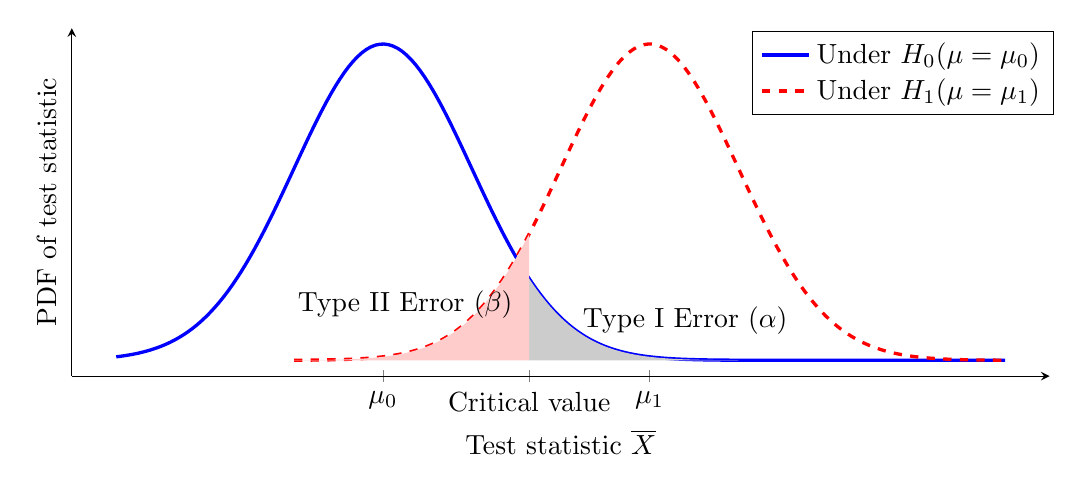
\begin{tikzpicture}
		\begin{axis}[
		domain=-3:7, samples=200,
		xlabel={ Test statistic $\overline{X}$ }, ylabel={PDF of test statistic},
		axis lines=left,
		height=6cm, width=14cm,
		xtick={0, 1.645, 3},
		xticklabels={$ \mu_0 $, Critical value, $ \mu_1 $},
		ytick=\empty,  % <-- remove y-ticks
		enlargelimits=0.05,
		legend style={at={(0.85,0.75)}, anchor=south}
		]

		% Null hypothesis distribution
		\addplot [very thick, blue] {1/sqrt(2*pi) * exp(-x^2/2)};
		\addlegendentry{Under $H_0 (\mu = \mu_0)$}

		% Alternative hypothesis distribution
		\addplot [very thick, red, dashed, domain=-1:7] {1/sqrt(2*pi) * exp(-(x-3)^2/2)};
		\addlegendentry{Under $H_1 (\mu = \mu_1)$}

		% Type I error region (right tail of H0)
		\addplot [
		domain=1.645:4,
		fill=gray!40,
		draw=none
		] {1/sqrt(2*pi) * exp(-x^2/2)} \closedcycle;
		\node at (axis cs:3.4,0.05) {Type I Error ($\alpha$)};

		% Type II error region (left of critical value under H1)
		\addplot [
		domain=-1:1.645,
		fill=red!20,
		draw=none
		] {1/sqrt(2*pi) * exp(-(x-3)^2/2)} \closedcycle;
		\node at (axis cs:0.25,0.07) {Type II Error ($\beta$)};

		\end{axis}
		\end{tikzpicture}
	\end{center}
	\caption{\textit{Type I and Type II error.}}
	\label{fig:type-i_and_type-ii}
\end{figure}

Here we assume the population parameter (i.e. population mean $\mu$) under $H_0$ is $\mu_0$ and under $H_1$ is a specific value\footnote{In practice, the specific value $\mu_1$ is unknown when the alternative hypothesis is specified as $H_1: \mu \neq \mu_0$. However, to compute the probability of a Type II error ($\beta$), we must assume a particular value of $\mu$ under the alternative hypothesis. This means that $\beta$ is not a single number, but rather a function of the true value of $\mu$ under $H_1$. For every possible value of $\mu_1$ under $H_1$, there is a corresponding value of $\beta$.} $\mu_1$.

Mathematically, for a given critical value \(c\):
\[
\alpha = P(\text{Reject } H_0 \mid H_0 \text{ true}) = P(T > c \mid H_0)
\]
\[
\beta = P(\text{Fail to reject } H_0 \mid H_1 \text{ true}) = P(T \le c \mid H_1)
\]

Changing the value of \(c\) affects \(\alpha\) and \(\beta\) in opposite ways, showing the trade-off between making Type I and Type II errors.


\begin{itemize}
	\item If we make the critical value \( c \) higher, the rejection region becomes smaller (more stringent), so \( \alpha \) will \textbf{decrease}, but \( \beta \) will \textbf{increase}.
	\item If we lower the value \( c \), the rejection region becomes larger (more liberal), so \( \alpha \) will \textbf{increase}, but \( \beta \) will \textbf{decrease}.
\end{itemize}

The Figure \ref{fig:alpha_beta_tradeoff} shows one typical example of the relationship between $\alpha$ and $\beta$.

\begin{figure}[H]
	\centering
	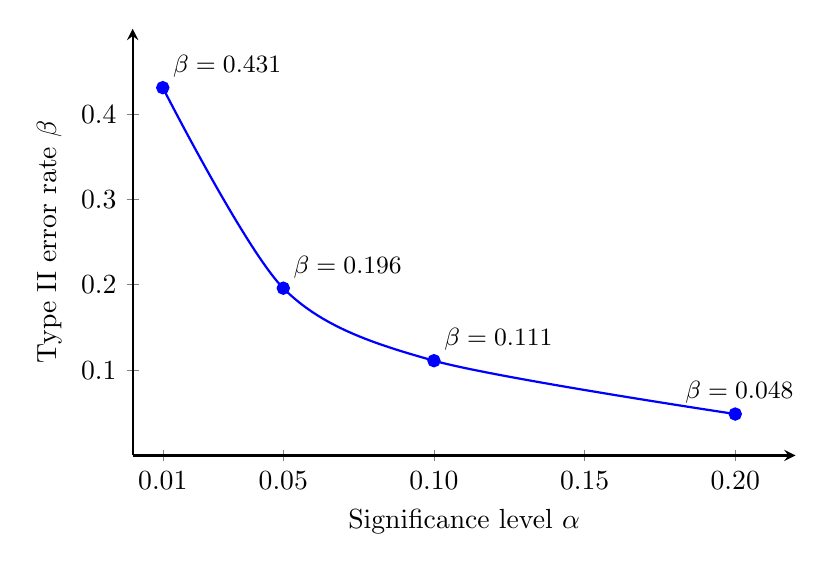
\begin{tikzpicture}
	\begin{axis}[
	width=10cm, height=7cm,
	%	domain=0:0.25,
	axis lines=left,
	xlabel={Significance level \(\alpha\)},
	ylabel={Type II error rate \(\beta\)},
	xmin=0, xmax=0.22,
	ymin=0, ymax=0.5,
	%tick align=outside,
	xtick={0.01, 0.05, 0.10, 0.15, 0.20},
	ytick={0.1, 0.2, 0.3, 0.4},
	xticklabels={0.01, 0.05, 0.10, 0.15, 0.20},
	thick
	%legend pos=north east,
	]
	% Plot the beta values directly as coordinates
	\addplot[smooth, thick, blue] coordinates {
		(0.01, 0.4310)
		(0.05, 0.1960)
		(0.10, 0.1110)
		(0.20, 0.0485)
	};
	%\addlegendentry{Effect size \(\delta = 2.5\)}

	% Mark points
	\addplot[only marks, mark=*, mark size=1.8pt, blue, very thick] coordinates {
		(0.01, 0.4310)
		(0.05, 0.1960)
		(0.10, 0.1110)
		(0.20, 0.0485)
	};

	% Annotate values
	\node[above right, font=\small] at (axis cs:0.01, 0.4310) {\(\beta = 0.431\)};
	\node[above right, font=\small] at (axis cs:0.05, 0.1960) {\(\beta = 0.196\)};
	\node[above right, font=\small] at (axis cs:0.10, 0.1110) {\(\beta = 0.111\)};
	\node[above right, font=\small] at (axis cs:0.18, 0.0485) {\(\beta = 0.048\)};
	\end{axis}
	\end{tikzpicture}
	\caption{\textit{Illustration of the inverse relationship between \(\alpha\) and \(\beta\).}}
	\label{fig:alpha_beta_tradeoff}
\end{figure}

Hence, a balance must be struck depending on the consequences of making Type I vs.\ Type II errors. To arrive at a fair compromise we should know the cost of each type of error. In practice, these costs depend on the true (but unknown) parameter and are hard to quantify exactly, so we adopt one of three conventional values—1\%, 5\%, or 10\%—based on the relative severity of each error.

For example, consider the design of an email spam filter. A \textbf{Type~I error} here means flagging a legitimate email as spam, potentially causing the user to miss important messages. A \textbf{Type~II error} would allow a spam message into the inbox, usually a minor nuisance. Thus, in this case, the cost of a Type I error is considered more serious than that of a Type II error, and the filter should be designed to minimize $\alpha$, the probability of Type~I error, even at the expense of a slightly higher $\beta$. A common choice might be $\alpha = 1\%$, to ensure that almost no valid emails are incorrectly filtered out.

On the other hand, imagine a public health agency conducting virus screening at airports during an outbreak of a contagious disease. A \textbf{Type~I error} in this context would mean falsely identifying a healthy traveler as infected, leading to temporary quarantine and inconvenience. A \textbf{Type~II error} would allow an infected traveler to enter the general population, potentially triggering a wider outbreak. In this scenario, the cost of a Type~II error is far more serious. To minimize this risk, we may choose a higher significance level, such as $\alpha = 10\%$, accepting more false positives in order to reduce the probability of missing actual infections.

Finally, in cases where the consequences of Type~I and Type~II errors are either unknown or roughly same, such as in exploratory scientific studiess, a balanced approach is often taken. The conventional significance level $\alpha = 5\%$ serves as a compromise that moderately controls both types of errors in the absence of more specific cost information.

\subsection{How $\beta$ Depends on the True Parameter Value?}
The probability of a Type II error ($\beta$) is not fixed; it varies depending on how far the actual parameter value is from the hypothesized value under $H_0$. Specifically:

\begin{itemize}
	\item If the true value is close to $H_0$, then the evidence against $H_0$ is weak, and $\beta$ is high (it’s harder to detect the difference).

	\item If the true value is far from $H_0$, then the evidence becomes stronger, and $\beta$ is lower (easier to detect the difference).
\end{itemize}
We generally write $\beta$ as a function of the parameter value $\theta_1$ under alternative hypothesis denoted by $\beta(\theta)$.

\subsection{Dependence on Sample Size}
Earlier, we discussed that one can choose a low $\alpha$ or a low $\beta$ depending on which type of error is more serious. But what if both Type I and Type II errors are costly, and we want to minimize both? The only effective way to achieve this is by improving the reliability of the evidence—primarily by increasing the sample size. As the sample size $n$ increases, the sampling distributions under both $H_0$ and $H_1$ become narrower (i.e., have smaller variance), which makes it easier to distinguish between them. This shrinkage leads to a reduction in both $\alpha$ and $\beta$. Therefore, when minimizing both types of error is important, increasing the sample size is the most practical solution.


\begin{figure}[H]
	\centering
	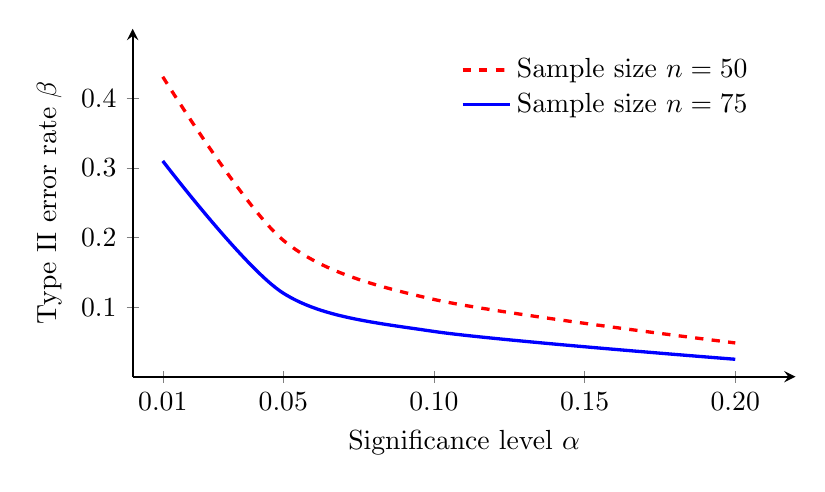
\begin{tikzpicture}
	\begin{axis}[
	width=10cm, height=6cm,
	axis lines=left,
	xlabel={Significance level \(\alpha\)},
	ylabel={Type II error rate \(\beta\)},
	xmin=0, xmax=0.22,
	ymin=0, ymax=0.5,
	xtick={0.01, 0.05, 0.10, 0.15, 0.20},
	ytick={0.1, 0.2, 0.3, 0.4},
	xticklabels={0.01, 0.05, 0.10, 0.15, 0.20},
	legend style={draw=none, at={(0.95,0.95)}, anchor=north east},
	thick
	]

	% Curve for n = 50
	\addplot[smooth, very thick, red, dashed] coordinates {
		(0.01, 0.4310)
		(0.05, 0.1960)
		(0.10, 0.1110)
		(0.20, 0.0485)
	};
	\addlegendentry{Sample size $n = 50$}


	% Curve for n = 75 (lower beta values due to larger sample)
	\addplot[smooth, very thick, blue] coordinates {
		(0.01, 0.3100)
		(0.05, 0.1200)
		(0.10, 0.0650)
		(0.20, 0.0250)
	};
	\addlegendentry{Sample size $n = 75$}

	\end{axis}
	\end{tikzpicture}
	\caption{\textit{Effect of sample size on the inverse relationship between \(\alpha\) and \(\beta\). Larger sample size reduces \(\beta\) for the same \(\alpha\).}}
	\label{fig:alpha_beta_sample_size}
\end{figure}



\subsection{$p$‐Value in Hypothesis Testing}

\begin{textbox}
The $p$\textbf{-value} is the probability, under null hypothesis, that the test statistic takes a value equal to or more extreme than the value actually observed.
\end{textbox}

Let $T$ be the test statistic used to assess $H_0$ versus $H_1$, and let $t_{\rm obs}$ be its observed value from the sample. Then for \textbf{one-sided test},
\[
p\text{-value} = P(T \ge t_{\rm obs}\mid H_0)
\]
For a \textbf{two‐sided test} (where both large and small values of $T$ count against $H_0$),
\begin{align*}
p\text{-value} &=
P(T \ge t_{\rm obs}\mid H_0)
\;+\;
P(T \le -\,t_{\rm obs}\mid H_0)
\end{align*}
Assuming the null distribution is symmetric:
\begin{align*}
p\text{-value} =2P(T \ge t_{\rm obs}\mid H_0)
\end{align*}

\begin{itemize}
	\item A \textbf{small} $p-$value (below the chosen significance level~$\alpha$) indicates that observing $t_{\rm obs}$ would be very unlikely if $H_0$ were true, so we \textbf{reject} $H_0$.
	\item A \textbf{large} $p-$value means the data are consistent with $H_0$, so we \textbf{fail to reject} $H_0$.
\end{itemize}

\begin{table}[H]
	\centering
	\vspace{0.5em}
	\renewcommand{\arraystretch}{1.5}
	\begin{tabular}{c|c}
		\toprule
		\textbf{Condition} & \textbf{Decision} \\
		\midrule
		$p\text{-value} \leq \alpha$  & Reject $H_0$ \\
		$p\text{-value} > \alpha$  & Fail to reject $H_0$ \\
		\bottomrule
	\end{tabular}
\caption{\textit{Decision rule based on $p$-value.}}
\end{table}

\paragraph{Example.}
Suppose $X_1,X_2,\dots,X_n\sim N(\mu,\sigma^2)$ with known $\sigma=0.3$, and we test
\[
H_0:\,\mu=5
\quad\text{vs.}\quad
H_1:\,\mu>5
\]
using
\[
T = \frac{\overline X - 5}{\sigma/\sqrt{n}}
\;\sim\; N(0,1)
\quad\text{under }H_0
\]
If $\overline X=5.1$, $n=36$, and $\sigma=0.3$, then
\[
t_{\rm obs}
= \frac{5.1 - 5}{0.3/\sqrt{36}}
= 2.00
\quad
\Rightarrow p\text{-value} = P(Z \ge 2.00) \approx 0.0228
\]
Since $p\text{-value}=0.0228<0.05$, we reject $H_0$ at 5\% level of significance.

% Always report the exact p‐value, not just “$p<0.05$,” to convey the strength of evidence.

\section{General Procedure for Hypothesis Testing}


	\subsubsection*{Step 1. Formulate the hypotheses}
	Formulate the {null hypothesis} ($H_0$), which represents the default claim about the population parameter, and the {alternative hypothesis} ($H_1$), which represents the effect or difference you aim to detect.

	\subsubsection*{Step 2. Choose a significance level}
	Select a level of significance $\alpha$ (commonly 0.01, 0.05, or 0.10) that defines the maximum probability of committing a Type I error (rejecting $H_0$ when it is true).

	\subsubsection*{Step 3. Define and calculate the test statistic}
	Identify an appropriate test statistic based on the hypotheses and assumption of population distribution. Then collect a sample of size $n$ and compute the observed value of the test statistic from the data.

	\subsubsection*{Step 4. Calculate the $ p $­-value or determine the critical value(s) from data}
	\begin{itemize}
		\item \emph{$ p $­-value approach:} Compute the probability, under $H_0$, of observing a test statistic at least as extreme as the one obtained.
		\item \emph{Critical value approach:} Identify the cutoff point(s) from the null distribution that correspond to the chosen $\alpha$, and define the rejection region(s).
	\end{itemize}

	\subsubsection*{Step 5. Make a decision}
	\begin{itemize}
		\item If the $ p $­-value is less than or equal to $\alpha$, \textbf{reject} $H_0$; otherwise, \textbf{do not reject} $H_0$.
		\item State the result in context, indicating whether there is sufficient evidence to support the alternative hypothesis at the chosen significance level.
	\end{itemize}

\section{Statistical Test for a Normally Distributed Population Mean \(\mu\)}

\subsection{Variance $\sigma^2$ Known}

\begin{enumerate}
	\item Hypothesis:
	$$H_0: \mu = \mu_0$$
	\begin{align*}
	H_1: \begin{cases}
	\mu > \mu_0, & \text{Right tail test}\\[6pt]
	\mu < \mu_0, & \text{Left tail test}\\[6pt]
	\mu \neq \mu_0, & \text{Two-sided test}\\[6pt]
	\end{cases}
	\end{align*}

	\item Select \(\alpha\) (commonly 0.01, 0.05, or 0.10) as the maximum probability of a Type I error.

	\item Test statistic
	\[
	Z \;=\;\frac{\overline{X} - \mu_0}{\sigma / \sqrt{n}}
	\]
	where \(\overline{X}\) is the sample mean, \(\sigma\) is known, and \(n\) is the sample size.  Under \(H_0\), \(Z \sim N(0,1)\). We then calculate the test statistic from the sample data. Let \(z_{\rm obs}\) is the observed value of \(Z\) from sample data.

	\item We now calculate the \(p\)-value from the distribution of test statistic:
		\[
		p\text{-value} =
		\begin{cases}
		P(Z \ge z_{\rm obs}), & \text{for }H_1:\mu>\mu_0\\[6pt]
		P(Z \le z_{\rm obs}), & \text{for }H_1:\mu<\mu_0\\[6pt]
		2\,P\bigl(|Z| \ge |z_{\rm obs}|\bigr), & \text{for }H_1:\mu\neq\mu_0
		\end{cases}
		\]
	Alternatively, we can identify the critical values and the rejection region at level $\alpha$:
	\begin{table}[H]
		\centering
		\begin{tabular}{@{}c|c|c@{}}
			\toprule
			\textbf{$H_1$} & \textbf{Critical Value(s)} & \textbf{Rejection Region} \\
			\midrule
			$\mu > \mu_0$ & $ z_{\alpha} $ &
			\(\{Z>z_{\alpha}\}\) \\[6pt]
			$\mu < \mu_0$ &
			$ -z_{\alpha} $ &
			\(\{Z<-z_{\alpha}\}\) \\[6pt]
			$\mu \neq \mu_0$ &
			$ \pm\,z_{\alpha/2} $&
			$\{|Z| > z_{\alpha/2}\}$ \\
			\bottomrule
		\end{tabular}
	\end{table}

	\item If \(p\text{-value} \le \alpha\), \textbf{reject} \(H_0\); otherwise, \textbf{do not reject} \(H_0\).

	Alternatively, if $z_{obs}$ lies in the rejection region, \textbf{reject} the \(H_0\); otherwise, \textbf{do not reject} \(H_0\).
\end{enumerate}

\textbf{Example}: A factory claims that their lightbulbs last an average of 1,000 hours. To verify this claim, a sample of lightbulbs is tested. The population standard deviation is assumed known as 50 hours.

\begin{itemize}
	\item Let \(\mu\) be the true mean lifetime of the lightbulbs (in hours).

	\item The null and alternative hypotheses are:
	\begin{align*}
	&H_0: \mu = 1000 \quad \text{(the claim is true)} \\
	&H_1: \mu \neq 1000 \quad \text{(the claim is false)}
	\end{align*}

	\item A random sample of \(n = 30\) lightbulbs is selected. The sample mean is \(\overline{X} = 980\) and the population standard deviation is assumed known as \(\sigma = 50\).

	\item Under the null hypothesis, the test statistic is:
	\[
	z_{\rm obs} = \dfrac{\overline{X} - \mu_0}{\sigma / \sqrt{n}}
	= \frac{980 - 1000}{50 / \sqrt{30}}
	= \frac{-20}{9.13} \approx -2.19
	\]

	\item From standard normal distribution tables, the two-tailed \(p\)-value is:
	\[
	p = 2 \cdot P(Z < -2.19) \approx 2 \cdot 0.0143 = 0.0286
	\]

	\item Since \(p < 0.05\), we reject the null hypothesis at the 5\% significance level. Thus there is statistically significant evidence at the 5\% level to suggest that the true average lifetime of the lightbulbs differs from 1,000 hours.
\end{itemize}


\subsection{Variance $\sigma^2 $ Unknown}

\begin{enumerate}
	\item Hypothesis:
	$$H_0: \mu = \mu_0$$
	\begin{align*}
	H_1: \begin{cases}
	\mu > \mu_0, & \text{Right tail test}\\[6pt]
	\mu < \mu_0, & \text{Left tail test}\\[6pt]
	\mu \neq \mu_0, & \text{Two-sided test}
	\end{cases}
	\end{align*}

	\item Select \(\alpha\) (commonly 0.01, 0.05, or 0.10) as the maximum probability of a Type I error.

	\item Test statistic:

	\begin{itemize}
		\item \textbf{Large sample} (\(n \ge 30\)):
		\[
		Z = \frac{\overline{X} - \mu_0}{S / \sqrt{n}}
		\]
		where \(S\) is the sample standard deviation.
		By the Central Limit Theorem, \(Z \sim N(0, 1)\) approximately under \(H_0\). Let \(z_{\rm obs}\) is the observed value of \(Z\) from sample data.

		\item \textbf{Small sample} (\(n < 30\)):
		\[
		T = \frac{\overline{X} - \mu_0}{S / \sqrt{n}}
		\]
		Here, \(T\) follows the \(t\)-distribution with \(n - 1\) degrees of freedom under \(H_0\). Let \(t_{\rm obs}\) is the observed value of \(T\) from sample data.
	\end{itemize}

	\item We now calculate the \(p\)-value from the distribution of the test statistic:

	\begin{itemize}
		\item \textbf{Large sample} (\(n \ge 30\)) — Use standard normal distribution:
		\[
		p\text{-value} =
		\begin{cases}
		P(Z \ge z_{\rm obs}), & \text{for }H_1:\mu>\mu_0,\\[6pt]
		P(Z \le z_{\rm obs}), & \text{for }H_1:\mu<\mu_0,\\[6pt]
		2\,P(|Z| \ge |z_{\rm obs}|), & \text{for }H_1:\mu\neq\mu_0
		\end{cases}
		\]

		\item \textbf{Small sample} (\(n < 30\)) — Use \(t\)-distribution with \(n-1\) degrees of freedom:
		\[
		p\text{-value} =
		\begin{cases}
		P(T \ge t_{\rm obs}), & \text{for }H_1:\mu>\mu_0,\\[6pt]
		P(T \le t_{\rm obs}), & \text{for }H_1:\mu<\mu_0,\\[6pt]
		2\,P(|T| \ge |t_{\rm obs}|), & \text{for }H_1:\mu\neq\mu_0
		\end{cases}
		\]
	\end{itemize}

Alternatively, identify critical values and rejection regions at level $\alpha$:

	\begin{itemize}

		\item \textbf{Large sample} (\(n \ge 30\))
		\begin{table}[H]
			\centering
			\begin{tabular}{@{}c|c|c@{}}
				\toprule
				\textbf{$H_1$} & \textbf{Critical Value(s)} & \textbf{Rejection Region} \\
				\midrule
				$\mu > \mu_0$ & $ z_{\alpha} $ &
				\(\{Z>z_{\alpha}\}\) \\[6pt]
				$\mu < \mu_0$ &
				$ -z_{\alpha} $ &
				\(\{Z<-z_{\alpha}\}\) \\[6pt]
				$\mu \neq \mu_0$ &
				$ \pm\,z_{\alpha/2} $&
				$\{|Z| > z_{\alpha/2}\}$ \\
				\bottomrule
			\end{tabular}
		\end{table}
	\item \textbf{Small sample} (\(n < 30\))
		\begin{table}[H]
			\centering
			\begin{tabular}{@{}c|c|c@{}}
				\toprule
				\textbf{$H_1$} & \textbf{Critical Value(s)} & \textbf{Rejection Region} \\
				\midrule
				$\mu > \mu_0$ & $ t_{\alpha,\,n-1} $ & $\{T > t_{\alpha,\,n-1}\}$ \\[6pt]
				$\mu < \mu_0$ & $ -t_{\alpha,\,n-1} $ & $\{T < -t_{\alpha,\,n-1}\}$ \\[6pt]
				$\mu \neq \mu_0$ & $ \pm\,t_{\alpha/2,\,n-1} $ & $\{|T| > t_{\alpha/2,\,n-1}\}$ \\
				\bottomrule
			\end{tabular}
		\end{table}
	\end{itemize}

	\item If \(p\text{-value} \le \alpha\), \textbf{reject} \(H_0\); otherwise, \textbf{do not reject} \(H_0\).

	Alternatively, if $t_{obs}$ (for large sample) or $t_{obs}$ (for small sample) lies in the rejection region, \textbf{reject} the \(H_0\); otherwise, \textbf{do not reject} \(H_0\).
\end{enumerate}


\section{Statistical Test for a Normally Distributed Population Variance \(\sigma^2\)}

\begin{enumerate}
	\item Hypothesis:
	$$H_0: \sigma^2 = \sigma_0^2$$
	\begin{align*}
	H_1: \begin{cases}
	\sigma^2 > \sigma_0^2, & \text{Right tail test}\\[6pt]
	\sigma^2 < \sigma_0^2, & \text{Left tail test}\\[6pt]
	\sigma^2 \neq \sigma_0^2, & \text{Two-sided test}\\[6pt]
	\end{cases}
	\end{align*}

	\item Select \(\alpha\) (commonly 0.01, 0.05, or 0.10) as the maximum probability of a Type I error.

	\item Test statistic
	\[
	\chi^2 = \frac{(n - 1) S^2}{\sigma_0^2}
	\]
	where \(S^2\) is the sample variance and \(n\) is the sample size. Under \(H_0\), \(\chi^2 \sim \chi^2_{n-1}\) (chi-squared distribution with \(n-1\) degrees of freedom). Let \(\chi^2_{\rm obs}\) be the observed value from the sample.

	\begin{figure}[H]
		\begin{center}
			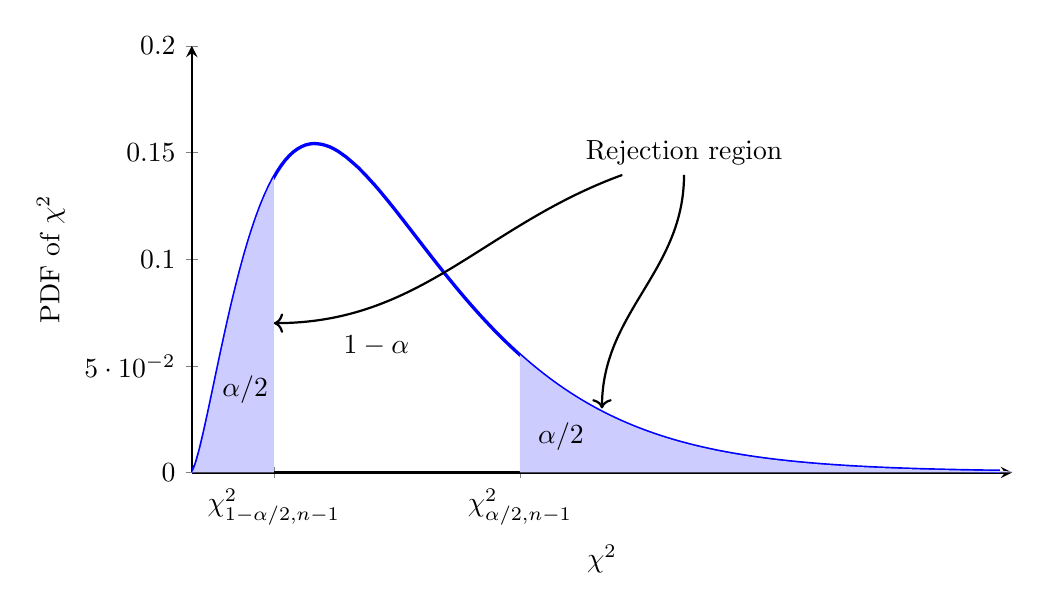
\begin{tikzpicture}
			\begin{axis}[
			width=12cm, height=7cm,
			domain=0:19.7, samples=200,
			axis lines=left,
			xlabel={$\chi^2$},
			ylabel={PDF of $\chi^2$},
			ymin=0, ymax=0.2,
			xmin=0, xmax=20,
			xtick={2,8},
			xticklabels={\(\chi_{1-\alpha/2, n-1}^2\), \(\chi_{\alpha/2, n-1}^2\)},
			% title={\small Chi-Squared Distributions for Different Degrees of Freedom},
			% grid=major,
			thick,
			]

			% ν = 5: f(x) = (1 / (2^{5/2} * Γ(5/2))) * x^{3/2} * exp(-x/2)
			% Γ(5/2) = 1.3293..., 2^{5/2} = 5.6568...
			% Constant = 1 / (5.6568 * 1.3293) ≈ 0.133
			\addplot [blue, very thick,] {0.133 * x^(1.5) * exp(-x/2)};

			% Shade the confidence interval region [-z_alpha/2, z_alpha/2]
			\addplot [
			domain=0:2,
			draw=none,
			fill=blue!20,
			samples=100
			]
			{0.133 * x^(1.5) * exp(-x/2)} \closedcycle;

			\addplot [
			domain=8:20,
			draw=none,
			fill=blue!20,
			samples=100
			]
			{0.133 * x^(1.5) * exp(-x/2)} \closedcycle;

			% Labels
			\node[below] at (axis cs:1.3,0.05) { ${\alpha/2}$};
			\node[below] at (axis cs:9,0.028) { ${\alpha/2}$};
			\node[above, black] at (axis cs:4.5,0.05) { \(1-\alpha\)};

			% Single label with two arrows
			\node (label) at (axis cs:12,0.15) {{Rejection region}};
			\draw[->, thick] (label) to[out=200,in=0] (axis cs:2,0.07);
			\draw[->, thick] (label) to[out=-90,in=90] (axis cs: 10,0.03);

			\end{axis}
			\end{tikzpicture}
			\caption{\textit{Critical values and rejection region for $\chi^2$ test statistic for two-sided test}.}
		\end{center}
	\end{figure}

	\item We now calculate the \(p\)-value from the distribution of the test statistic:
	\[
	p\text{-value} =
	\begin{cases}
	P(\chi^2 \ge \chi^2_{\rm obs}), & \text{for } H_1: \sigma^2 > \sigma_0^2 \\[6pt]
	P(\chi^2 \le \chi^2_{\rm obs}), & \text{for } H_1: \sigma^2 < \sigma_0^2 \\[6pt]
	2\,\min\bigl\{P(\chi^2 \le \chi^2_{\rm obs}),\; P(\chi^2 \ge \chi^2_{\rm obs})\bigr\}, & \text{for } H_1: \sigma^2 \neq \sigma_0^2
	\end{cases}
	\]

	In the two-sided test \( H_1: \sigma^2 \neq \sigma_0^2 \), we are interested in deviations of the sample variance from \( \sigma_0^2 \) in both directions. Since the chi-squared distribution is not symmetric, the two-tailed \( p \)-value is computed by taking the smaller of the two tail probabilities and double it, forming a conservative and valid two-sided p-value.
	This formula captures the probability of observing a value as extreme as \( \chi^2_{\text{obs}} \) in either tail of the distribution.

	Alternatively, we can use critical values and define the rejection region based on \(\alpha\):
	\begin{table}[H]
		\centering
		\begin{tabular}{@{}c|c|c@{}}
			\toprule
			\textbf{$H_1$} & \textbf{Critical Value(s)} & \textbf{Rejection Region} \\
			\midrule
			$\sigma^2 > \sigma_0^2$ & $\chi^2_{\alpha,\; n-1}$ &
			\(\{\chi^2 > \chi^2_{\alpha,\; n-1}\}\) \\[6pt]
			$\sigma^2 < \sigma_0^2$ &
			$\chi^2_{\alpha,\; n-1}$ &
			\(\{\chi^2 < \chi^2_{\alpha,\; n-1}\}\) \\[6pt]
			$\sigma^2 \neq \sigma_0^2$ &
			$\chi^2_{1-\alpha/2,\; n-1},\; \chi^2_{\alpha/2,\; n-1}$ &
			\(\{\chi^2 < \chi^2_{1-\alpha/2,\; n-1}\} \cup \{\chi^2 > \chi^2_{\alpha/2,\; n-1}\}\) \\
			\bottomrule
		\end{tabular}
	\end{table}

	\item If \(p\text{-value} \le \alpha\), \textbf{reject} \(H_0\); otherwise, \textbf{do not reject} \(H_0\).

	Alternatively, if \(\chi^2_{\rm obs}\) lies in the rejection region, \textbf{reject} \(H_0\); otherwise, \textbf{do not reject} \(H_0\).
\end{enumerate}

\section{Statistical Test for the Difference of Two Normally Distributed Population Means \(\mu_1 - \mu_2\)}

\subsection{Variances $\sigma_1^2$ and $\sigma_2^2$ Known}

\begin{enumerate}
	\item Hypothesis:
	$$H_0: \mu_1 - \mu_2 = \Delta_0$$
	\begin{align*}
	H_1: \begin{cases}
	\mu_1 - \mu_2 > \Delta_0, & \text{Right tail test}\\[6pt]
	\mu_1 - \mu_2 < \Delta_0, & \text{Left tail test}\\[6pt]
	\mu_1 - \mu_2 \neq \Delta_0, & \text{Two-sided test}
	\end{cases}
	\end{align*}
	where \(\Delta_0\) is the hypothesized difference (often 0).

	\item Select \(\alpha\) (commonly 0.01, 0.05, or 0.10) as the maximum probability of a Type I error.

	\item Test statistic
	\[
	Z \;=\; \frac{\overline{X}_1 - \overline{X}_2 - \Delta_0}{\sqrt{\dfrac{\sigma_1^2}{n_1} + \dfrac{\sigma_2^2}{n_2}}}
	\]
	where \(\overline{X}_1\) and \(\overline{X}_2\) are the sample means, \(\sigma_1^2\) and \(\sigma_2^2\) are the known population variances, and \(n_1\), \(n_2\) are the respective sample sizes. Under \(H_0\), \(Z \sim \mathcal{N}(0,1)\). Let \(z_{\rm obs}\) be the observed value of \(Z\) from the sample data.

	\item We now calculate the \(p\)-value from the distribution of the test statistic:
	\[
	p\text{-value} =
	\begin{cases}
	P(Z \ge z_{\rm obs}), & \text{for } H_1: \mu_1 - \mu_2 > \Delta_0 \\[6pt]
	P(Z \le z_{\rm obs}), & \text{for } H_1: \mu_1 - \mu_2 < \Delta_0 \\[6pt]
	2\,P\left(|Z| \ge |z_{\rm obs}|\right), & \text{for } H_1: \mu_1 - \mu_2 \neq \Delta_0
	\end{cases}
	\]

	Alternatively, we can identify the critical values and rejection regions at level \(\alpha\):
	\begin{table}[H]
		\centering
		\begin{tabular}{@{}c|c|c@{}}
			\toprule
			\textbf{$H_1$} & \textbf{Critical Value(s)} & \textbf{Rejection Region} \\
			\midrule
			$\mu_1 - \mu_2 > \Delta_0$ & $z_{\alpha}$ &
			\(\{Z > z_{\alpha}\}\) \\[6pt]
			$\mu_1 - \mu_2 < \Delta_0$ & $-z_{\alpha}$ &
			\(\{Z < -z_{\alpha}\}\) \\[6pt]
			$\mu_1 - \mu_2 \neq \Delta_0$ & $\pm z_{\alpha/2}$ &
			\(\{|Z| > z_{\alpha/2}\}\) \\
			\bottomrule
		\end{tabular}
	\end{table}

	\item If \(p\text{-value} \le \alpha\), \textbf{reject} \(H_0\); otherwise, \textbf{do not reject} \(H_0\).

	Alternatively, if \(z_{\rm obs}\) lies in the rejection region, \textbf{reject} \(H_0\); otherwise, \textbf{do not reject} \(H_0\).
\end{enumerate}


\subsection{Variances $\sigma_1^2$ and $\sigma_2^2$ Unknown}

\begin{enumerate}
	\item Hypothesis:
	$$H_0: \mu_1 - \mu_2 = \Delta_0$$
	\begin{align*}
	H_1: \begin{cases}
	\mu_1 - \mu_2 > \Delta_0, & \text{Right‐tail test}\\[6pt]
	\mu_1 - \mu_2 < \Delta_0, & \text{Left‐tail test}\\[6pt]
	\mu_1 - \mu_2 \neq \Delta_0, & \text{Two‐sided test}
	\end{cases}
	\end{align*}
	where \(\Delta_0\) is the hypothesized difference (often 0).

	\item Select \(\alpha\) (e.g.\ 0.01, 0.05, 0.10).

	\item Test statistic and degrees of freedom:

	\begin{description}[leftmargin=1cm]
		\item[(i) Equal variances assumed $\sigma_1^2=\sigma_2^2$ (pooled \(t\)–test)]
		\begin{align*}
		T \;&=\;\frac{\overline X_1 - \overline X_2 - \Delta_0}
		{\,S_p\sqrt{\dfrac1{n_1}+\dfrac1{n_2}}\,}
		\end{align*}
		where
		$$S_p^2 \;=\;\dfrac{(n_1-1)S_1^2 + (n_2-1)S_2^2}{\,n_1+n_2-2\,}$$
		is the pooled variance. Under $H_0$, $T$ follows a \(t\)-distribution with $\nu$ degrees freedom where $\nu=n_1+n_2-2$.

		\bigskip

		\item[(ii) Unequal variances assumed $\sigma_1^2\neq\sigma_2^2$ (Smith–Satterthwaite test)]
		$$T \;=\;
		\frac{\overline X_1 - \overline X_2 - \Delta_0}
		{\sqrt{\dfrac{S_1^2}{n_1} + \dfrac{S_2^2}{n_2}}}$$

		Under $H_0$, $T$ {approximately} follows a \(t\)-distribution with $\nu$ degrees of freedom (\textbf{Welch approximation}) where
		$$\nu \approx
		\dfrac{\left( \dfrac{S_1^2}{n_1}+\dfrac{S_2^2}{n_2}\right)^{2}}
		{\dfrac{(S_1^2/n_1)^2}{n_1-1} \;+\;\dfrac{(S_2^2/n_2)^2}{n_2-1}}$$
	\end{description}

	\item We now calculate the \(p\)-value using the appropriate \(t\)-distribution for test statistic:
	\[
	p\text{-value} =
	\begin{cases}
	P\bigl(T \ge t_{\rm obs}\bigr), & H_1:\,\mu_1-\mu_2 > \Delta_0\\[6pt]
	P\bigl(T \le t_{\rm obs}\bigr), & H_1:\,\mu_1-\mu_2 < \Delta_0\\[6pt]
	2\,P\bigl(|T|\ge |t_{\rm obs}|\bigr), & H_1:\,\mu_1-\mu_2 \neq \Delta_0
	\end{cases}
	\]

	Alternatively, we can identify the critical values and rejection regions at level \(\alpha\):

	\begin{table}[H]
		\centering
		\begin{tabular}{@{}c|c|c@{}}
			\toprule
			\textbf{$H_1$} & \textbf{Critical Value(s)} & \textbf{Rejection Region} \\
			\midrule
			\(\mu_1-\mu_2>\Delta_0\) &
			\(t_{1-\alpha,\;\nu}\) &
			\(\{T > t_{\alpha,\;\nu}\}\) \\[6pt]
			\(\mu_1-\mu_2<\Delta_0\) &
			\(-\,t_{\alpha,\;\nu}\) &
			\(\{T < -t_{\alpha,\;\nu}\}\) \\[6pt]
			\(\mu_1-\mu_2\neq\Delta_0\) &
			\(\pm\,t_{\alpha/2,\;\nu}\) &
			\(\{|T| > t_{\alpha/2,\;\nu}\}\) \\
			\bottomrule
		\end{tabular}
	\end{table}

	Here \(\nu = n_1+n_2-2\) for the pooled case, and \(\nu\) is given by the Welch–Satterthwaite formula for unequal variances.

	\item If \(p\text{-value}\le\alpha\), \textbf{reject} \(H_0\); otherwise, \textbf{do not reject} \(H_0\).
\end{enumerate}


\section{Statistical Test for the Ratio of Two Normally Distributed Population Variances}

\begin{enumerate}
	\item Let \(\sigma_1^2\) and \(\sigma_2^2\) be the variances of two independent normal populations. We want to test whether the ratio of these variances is equal to a specified positive value \(\delta\). The null and alternative hypotheses are:
	\[
	H_0: \frac{\sigma_1^2}{\sigma_2^2} = \delta
	\]
    \begin{align*}
    	H_1: \begin{cases}
    	{\sigma_1^2}/{\sigma_2^2} > \delta, & \text{Right tail test}\\[6pt]
    	{\sigma_1^2}/{\sigma_2^2} < \delta, & \text{Left tail test}\\[6pt]
    	{\sigma_1^2}/{\sigma_2^2} \neq \delta, & \text{Two-sided test}
    	\end{cases}
    \end{align*}

	\item Select \(\alpha\), the level of significance (e.g., 0.01, 0.05, or 0.10).

	\item Let \(S_1^2\) and \(S_2^2\) be the sample variances from independent random samples of sizes \(n_1\) and \(n_2\), respectively. The test statistic is:
	\[
	F = \dfrac{S_1^2}{\delta S_2^2}
	\]
	Under \(H_0\), \(F \sim F_{\nu_1,\nu_2}\), i.e., an F-distribution with \(\nu_1 = n_1 - 1\) and \(\nu_2 = n_2 - 1\) degrees of freedom. Let \(F_{\rm obs}\) be the observed value of the test statistic from the sample data.

	\item We now calculate the \(p\)-value from the F-distribution:
	\[
	p\text{-value} =
	\begin{cases}
	P(F \ge F_{\rm obs}), & \text{for } H_1: {\sigma_1^2}/{\sigma_2^2} > \delta \\[6pt]
	P(F \le F_{\rm obs}), & \text{for } H_1: {\sigma_1^2}/{\sigma_2^2} < \delta \\[6pt]
	2 \cdot \min\{P(F \ge F_{\rm obs}),\, P(F \le F_{\rm obs})\}, & \text{for } H_1: {\sigma_1^2}/{\sigma_2^2} \neq \delta
	\end{cases}
	\]

	Alternatively, use the critical values from the F-distribution at level \(\alpha\):

	\begin{table}[H]
		\centering
		\begin{tabular}{@{}c|c|c@{}}
			\toprule
			\textbf{$H_1$} & \textbf{Critical Value(s)} & \textbf{Rejection Region} \\
			\midrule
			\({\sigma_1^2}/{\sigma_2^2} > \delta\) &
			\(F_{\alpha;\,\nu_1,\nu_2}\) &
			\(\{F > F_{\alpha;\nu_1,\nu_2}\}\) \\[6pt]

			\({\sigma_1^2}/{\sigma_2^2} < \delta\) &
			\(F_{1-\alpha;\,\nu_1,\nu_2}\) &
			\(\{F < F_{1-\alpha;\nu_1,\nu_2}\}\) \\[6pt]

			\({\sigma_1^2}/{\sigma_2^2} \neq \delta\) &
			\(F_{1-\alpha/2;\,\nu_1,\nu_2},\, F_{\alpha/2;\,\nu_1,\nu_2}\) &
			\(\{F < F_{1-\alpha/2;\nu_1,\nu_2}\} \cup \{F > F_{\alpha/2;\nu_1,\nu_2}\}\)
			\\
			\bottomrule
		\end{tabular}
	\end{table}

	\item If \(p\text{-value} \le \alpha\), \textbf{reject} \(H_0\); otherwise, \textbf{do not reject} \(H_0\).

	Alternatively, if \(F_{\rm obs}\) lies in the rejection region, \textbf{reject} \(H_0\); otherwise, \textbf{do not reject} \(H_0\).
\end{enumerate}



\section{Statistical Test for a Population Proportion \(p\)}

\begin{enumerate}
	\item Let \(p\) be the true proportion of success in a Bernoulli population. We need to test whether this population proportion is equal to a specified value \(p_0\). The null and alternative hypotheses can be specified as:
	\[
	H_0: p = p_0
	\]
	\begin{align*}
	H_1: \begin{cases}
	p > p_0, & \text{Right tail test}\\[6pt]
	p < p_0, & \text{Left tail test}\\[6pt]
	p \neq p_0, & \text{Two-sided test}
	\end{cases}
	\end{align*}

	\item Select \(\alpha\) (e.g., 0.01, 0.05, or 0.10), the maximum allowable probability of a Type I error.

	\item Let \(\hat{p}\) be the sample proportion, based on a sample of size \(n\). Under \(H_0\), the test statistic is:
	\[
	Z = \frac{\hat{p} - p_0}{\sqrt{\dfrac{p_0(1 - p_0)}{n}}}
	\]
	which \textbf{approximately} follows the standard normal distribution \(\mathcal{N}(0,1)\) for sufficiently large \(n\) (typically \(np_0 \ge 5\) and \(n(1-p_0) \ge 5\)). Let \(z_{\rm obs}\) be the observed value of the test statistic.

	\item Compute the \(p\)-value using the standard normal distribution:
	\[
	p\text{-value} =
	\begin{cases}
	P(Z \ge z_{\rm obs}), & \text{for } H_1: p > p_0 \\[6pt]
	P(Z \le z_{\rm obs}), & \text{for } H_1: p < p_0 \\[6pt]
	2\,P\bigl(|Z| \ge |z_{\rm obs}|\bigr), & \text{for } H_1: p \neq p_0
	\end{cases}
	\]

	Alternatively, determine the rejection region using critical values from the standard normal distribution:

	\begin{table}[H]
		\centering
		\begin{tabular}{@{}c|c|c@{}}
			\toprule
			\textbf{$H_1$} & \textbf{Critical Value(s)} & \textbf{Rejection Region} \\
			\midrule
			\(p > p_0\) & \(z_{\alpha}\) & \(\{Z > z_{\alpha}\}\) \\[6pt]
			\(p < p_0\) & \(-z_{\alpha}\) & \(\{Z < -z_{\alpha}\}\) \\[6pt]
			\(p \neq p_0\) & \(\pm z_{\alpha/2}\) & \(\{|Z| > z_{\alpha/2}\}\) \\
			\bottomrule
		\end{tabular}
	\end{table}

	\item If \(p\text{-value} \le \alpha\), \textbf{reject} \(H_0\); otherwise, \textbf{do not reject} \(H_0\).

	Alternatively, if \(z_{\rm obs}\) lies in the rejection region, \textbf{reject} \(H_0\); otherwise, \textbf{do not reject} \(H_0\).
\end{enumerate}

\textbf{Example}: You suspect that a coin is biased. To test this, you flip the coin 100 times and observe 60 heads.

\begin{itemize}
	\item Let \(p\) be the true probability of getting heads.
	\item The null and alternative hypotheses are:
	\begin{align*}
	&H_0: p = 0.5 \quad \text{(the coin is fair)} \\
	&H_1: p \neq 0.5 \quad \text{(the coin is biased)}
	\end{align*}
	\item The sample proportion is \(\hat{p} = \dfrac{60}{100} = 0.6\).

	\item Under the null hypothesis, the test statistic is:
	\[
	z_{\rm obs} = \frac{\hat{p} - p_0}{\sqrt{\dfrac{p_0(1 - p_0)}{n}}}
	= \frac{0.6 - 0.5}{\sqrt{\dfrac{0.5 \times 0.5}{100}}}
	= \frac{0.1}{0.05} = 2.0
	\]

	\item From standard normal distribution tables, the two-tailed \(p\)-value is:
	\[
	p = 2 \cdot P(Z > 2.0) \approx 2 \cdot 0.0228 = 0.0456
	\]

	\item Since \(p < 0.05\), we reject the null hypothesis at the 5\% significance level. Therefore there is statistically significant evidence at the 5\% level to suggest that the coin may be biased.
\end{itemize}


\section{Power of a Test}

One very important concept related to error probabilities is the notion of the \emph{power} of a test. Intuitively, power measures a test's ability to detect when the null hypothesis is false. It is the probability of rejecting $ H_0 $ given that a specific alternative is true.

\begin{textbox}
	The \textbf{power} of a test at a specific alternative parameter value $\theta=\theta_1$ is defined as
	\begin{align*}
	\mathrm{Power}(\theta_1)=\gamma(\theta_1) &= P(\text{Rejecting }H_0\mid \theta = \theta_1)\\
	&=1-P(\text{Not rejecting }H_0\mid \theta = \theta_1)\\
	& = 1 - \beta(\theta_1)
	\end{align*}
Here $\beta(\theta_1)$ is the probability of a Type~II error when the true parameter equals $\theta_1$.
\end{textbox}
\bigskip

In other words, \textbf{it quantifies your test’s sensitivity to detect real departures from the null hypothesis}.

\subsection{Calculating Power in a One-Sample $Z$-Test}

\noindent\textbf{One-sided $Z$-test:} Consider testing
\[
H_0 : \mu = \mu_0 \quad \text{vs.} \quad H_1 : \mu > \mu_0,
\]
with known population standard deviation \( \sigma \), and a significance level \( \alpha \). The rejection region is:
\[
\overline{X} > \mu_0 + z_\alpha \cdot \frac{\sigma}{\sqrt{n}}.
\]

\noindent When the true mean is \( \mu = \mu_1 > \mu_0 \), the sampling distribution of \( \overline{X} \sim N(\mu_1, \sigma^2 / n) \), and the power is:
\[
\gamma(\mu_1) = P\left( \overline{X} > \mu_0 + z_\alpha \cdot \frac{\sigma}{\sqrt{n}}\right)
\]

\noindent Standardizing under \( H_1 \), we get:
\begin{align*}
\gamma(\mu_1) &=P\left( \dfrac{\overline{X}-\mu_1}{\sigma/\sqrt{n}} > \dfrac{1}{\sigma/\sqrt{n}}\left( \mu_0 + z_\alpha \cdot \frac{\sigma}{\sqrt{n}}-\mu_1\right)  \right) \\
&= P\left( Z > z_\alpha - \frac{(\mu_1 - \mu_0)\sqrt{n}}{\sigma} \right)
\end{align*}

\medskip

\noindent\textbf{Two-Sided $Z$-Test}: Now consider the two-sided alternative:
\[
H_0 : \mu = \mu_0 \quad \text{vs.} \quad H_1 : \mu \ne \mu_0.
\]

with known population standard deviation \( \sigma \), and a significance level \( \alpha \). The rejection region is:
\[
\overline{X} < \mu_0 - z_{\alpha/2} \cdot \frac{\sigma}{\sqrt{n}} \quad \text{or} \quad
\overline{X} > \mu_0 + z_{\alpha/2} \cdot \frac{\sigma}{\sqrt{n}}
\]

If the true mean is \( \mu = \mu_1 \ne \mu_0 \), then:
\begin{align*}
\gamma(\mu_1) &= P\left( \overline{X} < \mu_0 - z_{\alpha/2} \cdot \frac{\sigma}{\sqrt{n}} \right)
+ P\left( \overline{X} > \mu_0 + z_{\alpha/2} \cdot \frac{\sigma}{\sqrt{n}} \right)
\end{align*}

Standardizing:
\begin{align*}
\gamma(\mu_1)
&= P\left( Z < -z_{\alpha/2} - \frac{(\mu_1 - \mu_0)\sqrt{n}}{\sigma} \right)
+ P\left( Z > z_{\alpha/2} - \frac{(\mu_1 - \mu_0)\sqrt{n}}{\sigma} \right),
\end{align*}
where again \( Z \sim N(0,1) \)

\medskip
In both cases, we observed the following factors affecting power in the $Z$-test:
\begin{itemize}
  \item \textbf{Significance level \( \alpha \):} Increasing \( \alpha \) increases power.
  \item \textbf{Effect size \( \mu_1 - \mu_0 \):} Larger differences are easier to detect.
  \item \textbf{Population standard deviation \( \sigma \):} Smaller \( \sigma \) increases power.
  \item \textbf{Sample size \( n \):} Increasing \( n \) increases power by reducing standard error.
\end{itemize}

\textbf{Example}: The power of a two‐sided $Z$‐test ($H_0: \mu = 5$ vs.\ $H_1: \mu \neq 5$) with known $\sigma = 0.3$, $n = 50$, and $\alpha = 0.05$ is the probability it will reject $H_0$ when $\mu$ truly equals $4.8$.  Here the critical region is
\[
\overline{X} < 4.9168
\quad\text{or}\quad
\overline{X} > 5.0832
\]
If in reality $\mu = 4.8$, then
\[
\overline{X} \sim N\bigl(4.8,\;\mathrm{SE}^2\bigr),
\]
and
\[
P\bigl(\overline{X} < 4.9168\bigr)
= F_Z\Bigl(\frac{4.9168 - 4.8}{0.04243}\Bigr)
\approx 0.9971
\]
while
\[
P\bigl(\overline{X} > 5.0832\bigr)
= 1 - F_Z\Bigl(\frac{5.0832 - 4.8}{0.04243}\Bigr)
\approx 0
\]
Thus the test’s power at $\mu = 4.8$ is
$$\gamma(4.8) = P\bigl(\overline{X} < 4.9168\bigr)+P\bigl(\overline{X} > 5.0832\bigr) = 0.9971\ (\approx 99.7\%)$$
meaning there’s a 99.7\% chance (very sensitive) of detecting this 0.2‑unit shift.


\begin{figure}[H]
\centering
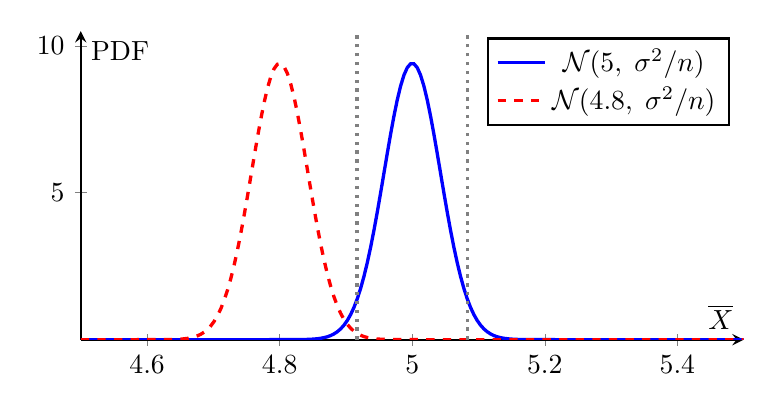
\begin{tikzpicture}
  \begin{axis}[
      domain=4.5:5.5, samples=200,
      axis lines=middle,
      xlabel={$\overline{X}$}, ylabel={PDF},
      ymin=0, ymax=10.5,
      width=10cm, height=5.5cm,
      legend style={at={(0.98,0.98)}, anchor=north east},
      thick
    ]
    % parameters
    \pgfmathsetmacro\muo{5}
    \pgfmathsetmacro\mui{4.8}
    \pgfmathsetmacro\se{0.3/sqrt(50)}

    % H0 density
    \addplot[blue, very thick] {1/(\se*sqrt(2*pi))*exp(-((x-\muo)^2)/(2*\se^2))};
    \addlegendentry{$\mathcal{N}(5,\;\sigma^2/n)$}

    % H1 density
    \addplot[red, very thick, dashed] {1/(\se*sqrt(2*pi))*exp(-((x-\mui)^2)/(2*\se^2))};
    \addlegendentry{$\mathcal{N}(4.8,\;\sigma^2/n)$}

    % critical values
    \def\cL{4.9168}
    \def\cU{5.0832}
    \addplot[dotted, gray, very thick] coordinates {(\cL,0) (\cL,12)};
    \addplot[dotted, gray, very thick] coordinates {(\cU,0) (\cU,12)};
    \node[gray] at (axis cs:\cL,12) [anchor=south] {$4.9168$};
    \node[gray] at (axis cs:\cU,12) [anchor=south] {$5.0832$};

    % Shade power region under H1 left tail
    \addplot[red!30, draw=none, domain=4.5:\cL]
      {1/(\se*sqrt(2*pi))*exp(-((x-\mui)^2)/(2*\se^2))} \closedcycle;
    % Shade power region under H1 right tail
    \addplot[red!30, draw=none, domain=\cU:5.5]
      {1/(\se*sqrt(2*pi))*exp(-((x-\mui)^2)/(2*\se^2))} \closedcycle;

  \end{axis}
\end{tikzpicture}
\caption{\textit{Density curves for \(H_0: \mu=5\) and \(H_1: \mu=4.8\) with \(\sigma=0.3\), \(n=50\).  The dashed lines at 4.9168 and 5.0832 are the critical cutoffs; the shaded regions under the \(H_1\) curve indicate the power ($\approx$ 99.7\%).}}
\end{figure}


Higher power can be achieved by increasing the sample size, accepting a larger $\alpha$, or targeting a larger effect size. Before running an experiment, one often conducts a power analysis to choose \(n\) (or \(\alpha\)) so that the power exceeds a desired threshold (commonly 0.8 or 0.9) for a specified effect size.

\begin{figure}[H]
\centering
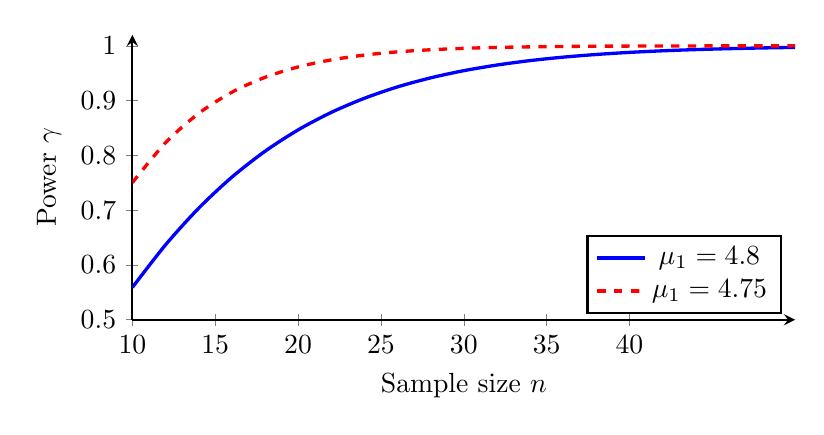
\begin{tikzpicture}
  \begin{axis}[
      xlabel={Sample size \(n\)},
      ylabel={Power \(\gamma\)},
      axis lines=left,
      xmin=10, xmax=50,
      ymin=0.5, ymax=1.02,
      xtick={10,15,20,25,30,35,40},
      ytick={0.5,0.6,0.7,0.8,0.9,1.0},
      width=10cm, height=5.2cm,
      thick,
      legend style={at={(0.98,0.02)}, anchor=south east},
      mark options={solid, scale=0.5},
    ]
    \addplot[
      blue,
      smooth, very thick
    ] coordinates {
      (10, 0.5589) (12, 0.6366) (14, 0.7035) (16, 0.7601) (18, 0.8074) (20, 0.8465) (22, 0.8784) (24, 0.9042) (26, 0.9250) (28, 0.9415) (30, 0.9546) (32, 0.9649) (34, 0.9730) (36, 0.9793) (38, 0.9842) (40, 0.9880) (42, 0.9909) (44, 0.9931) (46, 0.9948) (48, 0.9961) (50, 0.9971)
    };
    \addlegendentry{\(\mu_1 = 4.8\)}

    \addplot[
      red,
      smooth, very thick, dashed
    ] coordinates {
      (10, 0.7502) (12, 0.8230) (14, 0.8766) (16, 0.9152) (18, 0.9424) (20, 0.9614) (22, 0.9743) (24, 0.9831) (26, 0.9890) (28, 0.9928) (30, 0.9954) (32, 0.9971) (34, 0.9981) (36, 0.9988) (38, 0.9993) (40, 0.9995) (42, 0.9997) (44, 0.9998) (46, 0.9999) (48, 0.9999) (50, 1.0000)
    };
    \addlegendentry{\(\mu_1 = 4.75\)}
  \end{axis}
\end{tikzpicture}
\caption{\textit{Power curve for the two-sided \(Z\)-test in the above example with \(\mu_0 = 5\), \(\sigma = 0.3\), \(\alpha = 0.05\), showing power curves for \(\mu_1 = 4.8\) and \(\mu_1 = 4.75\) as sample size \(n\) varies from 10 to 40.}}
\end{figure}


\begin{figure}[H]
\centering
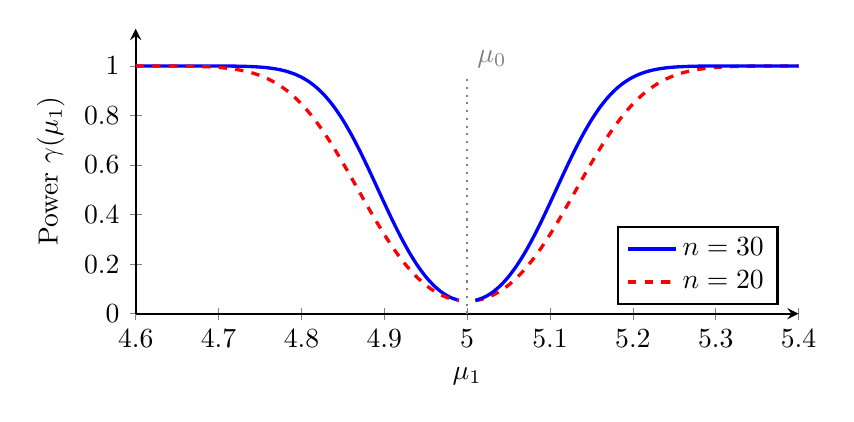
\begin{tikzpicture}
  \begin{axis}[
      xlabel={$\mu_1$},
      ylabel={Power $\gamma(\mu_1)$},
      axis lines=left,
      xmin=4.6, xmax=5.4,
      ymin=0, ymax=1.15,
      xtick={4.5,4.6,4.7,4.8,4.9,5.0,5.1,5.2,5.3,5.4,5.5},
      ytick={0,0.2,0.4,0.6,0.8,1.0},
      width=10cm, height=5.2cm,
      thick,
      mark options={solid, scale=0.6},
      legend pos=south east,
    ]
    \addplot[
      blue,
      very thick,
      smooth
    ] coordinates {
      (4.60, 1.0000) (4.61, 1.0000) (4.62, 1.0000) (4.63, 1.0000) (4.64, 1.0000) (4.65, 1.0000) (4.66, 1.0000) (4.67, 1.0000) (4.68, 0.9999) (4.69, 0.9999) (4.70, 0.9998) (4.71, 0.9996) (4.72, 0.9992) (4.73, 0.9985) (4.74, 0.9973) (4.75, 0.9954) (4.76, 0.9923) (4.77, 0.9874) (4.78, 0.9801) (4.79, 0.9695) (4.80, 0.9546) (4.81, 0.9343) (4.82, 0.9076) (4.83, 0.8736) (4.84, 0.8318) (4.85, 0.7819) (4.86, 0.7244) (4.87, 0.6604) (4.88, 0.5913) (4.89, 0.5193) (4.90, 0.4467) (4.91, 0.3759) (4.92, 0.3091) (4.93, 0.2482) (4.94, 0.1948) (4.95, 0.1496) (4.96, 0.1130) (4.97, 0.0850) (4.98, 0.0654) (4.99, 0.0538)
    };
    \addlegendentry{\(n=30\)}
    \addplot[
                  red,
                  very thick,
                  smooth, dashed
                ] coordinates {
                  (5.01, 0.0525) (5.02, 0.0602) (5.03, 0.0732) (5.04, 0.0916) (5.05, 0.1157) (5.06, 0.1455) (5.07, 0.1810) (5.08, 0.2222) (5.09, 0.2687) (5.10, 0.3197) (5.11, 0.3746) (5.12, 0.4322) (5.13, 0.4913) (5.14, 0.5506) (5.15, 0.6088) (5.16, 0.6647) (5.17, 0.7171) (5.18, 0.7653) (5.19, 0.8085) (5.20, 0.8465) (5.21, 0.8791) (5.22, 0.9065) (5.23, 0.9290) (5.24, 0.9471) (5.25, 0.9614) (5.26, 0.9723) (5.27, 0.9805) (5.28, 0.9866) (5.29, 0.9909) (5.30, 0.9940) (5.31, 0.9961) (5.32, 0.9975) (5.33, 0.9985) (5.34, 0.9991) (5.35, 0.9994) (5.36, 0.9997) (5.37, 0.9998) (5.38, 0.9999) (5.39, 0.9999) (5.40, 1.0000) (5.41, 1.0000)
                };
    \addlegendentry{\(n=20\)}
    \addplot[
          blue,
          very thick,
          smooth
        ] coordinates {
          (5.01, 0.0538) (5.02, 0.0654) (5.03, 0.0850) (5.04, 0.1130) (5.05, 0.1496) (5.06, 0.1948) (5.07, 0.2482) (5.08, 0.3091) (5.09, 0.3759) (5.10, 0.4467) (5.11, 0.5193) (5.12, 0.5913) (5.13, 0.6604) (5.14, 0.7244) (5.15, 0.7819) (5.16, 0.8318) (5.17, 0.8736) (5.18, 0.9076) (5.19, 0.9343) (5.20, 0.9546) (5.21, 0.9695) (5.22, 0.9801) (5.23, 0.9874) (5.24, 0.9923) (5.25, 0.9954) (5.26, 0.9973) (5.27, 0.9985) (5.28, 0.9992) (5.29, 0.9996) (5.30, 0.9998) (5.31, 0.9999) (5.32, 0.9999) (5.33, 1.0000) (5.34, 1.0000) (5.35, 1.0000) (5.36, 1.0000) (5.37, 1.0000) (5.38, 1.0000) (5.39, 1.0000) (5.40, 1.0000) (5.41, 1.0000)
        };
    \draw[dotted, gray] (axis cs:5.0,0) -- (axis cs:5.0,0.95) node[above right]{$\mu_0$};

    \addplot[
          red,
          very thick,
          smooth, dashed
        ] coordinates {
          (4.60, 1.0000) (4.61, 0.9999) (4.62, 0.9999) (4.63, 0.9998) (4.64, 0.9997) (4.65, 0.9994) (4.66, 0.9991) (4.67, 0.9985) (4.68, 0.9975) (4.69, 0.9961) (4.70, 0.9940) (4.71, 0.9909) (4.72, 0.9866) (4.73, 0.9805) (4.74, 0.9723) (4.75, 0.9614) (4.76, 0.9471) (4.77, 0.9290) (4.78, 0.9065) (4.79, 0.8791) (4.80, 0.8465) (4.81, 0.8085) (4.82, 0.7653) (4.83, 0.7171) (4.84, 0.6647) (4.85, 0.6088) (4.86, 0.5506) (4.87, 0.4913) (4.88, 0.4322) (4.89, 0.3746) (4.90, 0.3197) (4.91, 0.2687) (4.92, 0.2222) (4.93, 0.1810) (4.94, 0.1455) (4.95, 0.1157) (4.96, 0.0916) (4.97, 0.0732) (4.98, 0.0602) (4.99, 0.0525)
        };


  \end{axis}
\end{tikzpicture}
\caption{\textit{Power curve of the two-sided $Z$-test in the above example as the true mean $\mu_1$ varies  with \(\mu_0=5\), \(\sigma=0.3\), and \(\alpha=0.05\). The vertical dashed line marks the null value $\mu_0=5$. The value of $\gamma(\mu_1)$ as $\mu_1 \to \mu_0$ is $\alpha =0.05$. Because this is the probability of rejecting $H_0$ when it is actually true which happens when $\mu_1 \to \mu_0$.}}
\end{figure}



\subsection{Required Sample Size for a One-Sample $Z$-Test}

\textbf{One-sided $Z$-test}: When planning a one-sided $Z$-test
\[
H_0: \mu = \mu_0
\quad\text{versus}\quad
H_1: \mu > \mu_0,
\]
we wish to choose \(n\) so that the power at \(\mu>\mu_1 \neq \mu_0\) is
\(\gamma = 1-\beta\).  Recall that
\[
\gamma(\mu_1)
= P\Bigl(Z > z_\alpha - \dfrac{(\mu_1-\mu_0)\sqrt{n}}{\sigma}\Bigr)
\]
By the definition of \(z_\beta\),
$$P(Z>z_\beta)=\beta \quad \Longrightarrow 1-\beta = 1-P(Z>z_\beta)=P(Z<z_\beta)=P(Z>-z_\beta)$$

Thus we can write
\[
z_\alpha - \frac{(\mu_1-\mu_0)\sqrt{n}}{\sigma} \;=\; -z_\beta
\]
Solving for \(n\) gives the minimum sample size needed:
\[
n \;=\;
\left(\frac{z_\alpha + z_\beta}{(\mu_1 - \mu_0)/\sigma}\right)^{\!2}
\;=\;
\left(\frac{z_\alpha + z_\beta}{\delta}\right)^2
\]
where $\delta = \dfrac{\mu_1-\mu_0}{\sigma}$ is the standardize effect size. The same formula applies when the alternative hypothesis is \(H_1: \mu < \mu_0\).

\noindent Thus, to achieve significance level \(\alpha\) and power \(1-\beta\)
against a shift of \(\mu_1-\mu_0\), one needs
\[
n \;\ge\; \left(\frac{z_\alpha + z_\beta}{\delta}\right)^2
\]

\textbf{Two-sided $Z$-test}: In two-sided tests, a closed-form expression for the required sample size is generally not available and is therefore best performed using statistical software.


\subsection{Receiver Operating Characteristic (ROC) Curve}

The ROC curve is the plot of the true positive rate (TPR) against the false positive rate (FPR) for different thresholds of a test statistic.

\begin{itemize}
	\item \textbf{True Positive Rate (TPR) or Sensitivity:} \(1 - \beta = P(\text{Reject } H_0 \mid H_1 \text{ true})\).
	\item \textbf{False Positive Rate (FPR):} \(\alpha = P(\text{Reject } H_0 \mid H_0 \text{ true})\).
\end{itemize}

By varying the critical value \(c\), we obtain different pairs \((\alpha, 1-\beta)\), which can be plotted with \(\alpha\) on the x-axis and power on the y-axis to produce the ROC curve.

\begin{figure}[H]
\begin{center}
	\begin{tikzpicture}[scale=1.2]
	\draw[->, thick] (0,0) -- (5,0) node[right] {False Positive Rate (\(\alpha\))};
	\draw[->, thick] (0,0) -- (0,5) node[above] {True Positive Rate (Power)};

	% Diagonal line (random guess line)
	\draw[dotted, gray, thick] (0,0) -- (4.5,4.5);

	% Example ROC curve (concave)
	\draw[very thick, blue] plot [smooth] coordinates {(0,0) (0.5,1.2) (1.5,3.1) (2.5,3.8) (4.5,4.5)};

    % Example ROC curve (concave)
    \draw[very thick, red, dashed] plot [smooth] coordinates {(0,0) (0.5,0.8) (1.5,2.2) (2.5,3.2) (4.5,4.5)};

	% Points
	\filldraw (0,0) circle (1.5pt) node[below left] {0};
	\filldraw (4.5,4.5) circle (1.5pt) node[above right] {1};

	% Labels
	\node at (1.9,4) {Large sample};
    \node at (3.3,3.0) {Small sample};
	\node[gray] at (3.2,2.0) {Random Guess};
	\end{tikzpicture}
\end{center}
\caption{\textit{ROC curves for two sample sizes.}}
\label{fig:roc}
\end{figure}

The ROC curve helps us visualize and compare the effectiveness of tests across different thresholds. The closer the ROC curve approaches the top-left corner, the better the test's ability to discriminate between \(H_0\) and \(H_1\). From the Figure~\ref{fig:roc}, we can see as the sample size increases, the ROC curve moves closer to the top-left corner, indicating improved test power and discrimination ability.

The \textbf{Area Under the Curve (AUC)} quantifies overall test performance: an AUC of 1 indicates perfect discrimination, whereas an AUC of 0.5 corresponds to random guessing.

\chapter{Correlation and Regression}

\section{Correlation}

\begin{textbox}
In statistics, \textbf{correlation} between two random variables is a measure of the degree of linear association between them.
\end{textbox}
 For example, imagine you record how many hours each of the six students studies in a week and their corresponding exam scores:

\begin{table}[h!]
	\centering
	\begin{tabular}{c|c|c}
		\toprule
		\textbf{Student} & \textbf{Hours Studied} ($X$) & \textbf{Exam Score} ($Y$) \\
		\midrule
		1 & 2 & 65 \\
		2 & 3 & 70 \\
		3 & 4 & 76 \\
		4 & 5 & 78 \\
		5 & 6 & 82 \\
		6 & 7 & 89 \\
		\bottomrule
	\end{tabular}
	\caption{\textit{Study hours and exam scores of six students.}}
	\label{tab:study_scores}
\end{table}

\begin{figure}[h!]
	\centering
	\begin{tikzpicture}
	\begin{axis}[
	xlabel={Hours Studied},
	ylabel={Exam Score},
	axis lines=left,
	xmin=1, xmax=8, ymin=60, ymax=95 ,
	width=10cm,
	height=5cm,
	thick,
	]
	\addplot[only marks, blue, mark=*, mark size=2pt] coordinates {
		(2,65) (3,70) (4,76) (5,78) (6,82) (7,89)
	};
	\end{axis}
	\end{tikzpicture}
	\caption{\textit{Scatter plot of study time and exam performance.}}
\end{figure}


As illustrated in the table and the accompanying scatter plot, exam scores increase as students dedicate more hours to studying. This clear upward pattern reflects a positive correlation: students who invest more time in preparation tend to achieve higher marks.  In general, the direction of correlation can be classified as follows:

\begin{enumerate}
	\item \textbf{Positive correlation}: An increase in one variable is accompanied by an increase in the other.
	\item \textbf{Negative correlation}: An increase in one variable is accompanied by a decrease in the other.
	\item \textbf{No (zero) correlation}: Changes in one variable show no consistent association with changes in the other.
\end{enumerate}


\section{Pearson Correlation Coefficient}

Pearson's correlation coefficient for a population, commonly denoted by the Greek letter \(\rho\) (rho), is also known as the \textbf{population correlation coefficient}. Given a pair of random variables \(X\) and \(Y\), the population correlation coefficient \(\rho_{XY}\) is defined as

\begin{textbox}
\[
\rho_{XY} = \frac{\operatorname{Cov}(X,Y)}{\sigma_X \sigma_Y} = \frac{\mathbb{E}\big[(X - \mu_X)(Y - \mu_Y)\big]}{\sigma_X \sigma_Y}
\]
\end{textbox}
where \(\mu_X = \mathbb{E}[X]\) and \(\mu_Y = \mathbb{E}[Y]\) are the means of \(X\) and \(Y\), \(\sigma_X\) and \(\sigma_Y\) are their standard deviations, and \(\operatorname{Cov}(X,Y)\) is the covariance between \(X\) and \(Y\).

Like all population parameters, The value of $\rho_{XY}$ is not known to us. We may need to estimate it from the random sample observation pairs $(X,Y)$. Let $$ (x_1, y_1), (x_2, y_2), \dots,(x_n, y_n) $$ be $n$ pairs of observations with respective means $\overline{X}, \overline{Y}$ and variances $S_X^2, S_X^2$ respectively. It turns out that a point estimate of $\text{Cov}(X,Y)$ is the sample covariance:
$$ S_{XY} = \dfrac{\sum_{i=1}^{n} (x_i - \overline{x})(y_i - \overline{y})}{n-1} $$
The point estimate of $\sigma_X$ is sample standard deviation of $X$:
$$S_X = \sqrt{\dfrac{1}{n - 1} \sum_{i=1}^{n} (x_i - \overline{x})^2}$$
The point estimate of $\sigma_Y$ is sample standard deviation of $Y$:
$$S_Y = \sqrt{\dfrac{1}{n - 1} \sum_{i=1}^{n} (y_i - \overline{y})^2}$$

Substituting these estimates for their population counterparts, we get the formula for the \textbf{sample correlation coefficient} as

\begin{textbox}
	\[
	r_{XY} = \dfrac{S_{XY}}{S_X \cdot S_Y}
	\]
\end{textbox}
Alternatively, $r_{XY}$ can be expressed as
\begin{textbox}
\[
r_{XY} = \dfrac{\sum_{i=1}^{n} (x_i - \overline{x})(y_i - \overline{y})}{\sqrt{\sum_{i=1}^{n} (x_i - \overline{x})^2} \sqrt{\sum_{i=1}^{n} (y_i - \overline{y})^2}}
\]
\end{textbox}

We can simplify the formula for $r_{XY}$ into a form most convenient for computing from raw data by using the identities:
\begin{align*}
\sum_i (x_i - \overline{x})(y_i - \overline{y}) &= \sum_i x_i y_i - n\overline{x}\cdot \overline{y} = \sum_i x_i y_i - \frac{\sum_i x_i \sum_i y_i}{n} \\
\sum_i (x_i - \overline{x})^2 &= \sum_i x_i^2 -n\overline{x}^2= \sum_i x_i^2 - \frac{(\sum_i x_i)^2}{n} \\
\sum_i (y_i - \overline{y})^2 &= \sum_i y_i^2 -n\overline{y}^2= \sum_i y_i^2 - \frac{(\sum_i y_i)^2}{n}
\end{align*}

Thus we obtain the formula for $r_{XY}$:
\begin{textbox}
\begin{align*}
r_{XY} = \frac{n \sum x_i y_i - \sum x_i \sum y_i}
{\sqrt{n \sum x_i^2 - (\sum x_i)^2} \cdot \sqrt{n \sum y_i^2 - (\sum y_i)^2}}
\end{align*}
\end{textbox}

The value of $r_{XY}$ lies within -1 and 1 i.e. $-1 \leq r_{XY} \leq 1$.
\begin{textbox}
\begin{itemize}
	\item $r > 0$ indicates a \textbf{positive correlation}.
	\item $r < 0$ indicates a \textbf{negative correlation}.
	\item $r = 0$ suggests \textbf{no correlation} (but not necessarily independence).
	\item $r = \pm 1$ indicates a \textbf{perfect linear correlation} ($+1$ for positive and $-1$ for negative).
\end{itemize}
\end{textbox}

% In your document preamble:
%   \usepackage{pgfplots}
%   \pgfplotsset{compat=1.17}
%   \usepgfplotslibrary{groupplots}

\begin{figure}[h!]
	\centering
	\begin{tikzpicture}
	\begin{groupplot}[
	group style={
		group size=2 by 2,
		horizontal sep=3cm,
		vertical sep=2cm
	},
	width=5cm,
	height=4cm,
	axis lines=left,
	axis line style={thick},
	xlabel={$X$},
	ylabel={$Y$},
	tick align=outside,
	]
	% Positive correlation
	\nextgroupplot[title={Positive Correlation ($r>0$)},xmin=0, xmax=8,	ymin=1]
	\addplot[only marks, blue, mark=*, mark size=1.5pt] coordinates {
		(1,1.5) (2,1.9) (3,3.1) (4,4.8) (5,4.9) (6,5.9) (7,7.8)
	};

	% Negative correlation
	\nextgroupplot[title={Negative Correlation ($r<0$)},xmin=0, xmax=8,	ymin=1]
	\addplot[only marks, blue, mark=*, mark size=1.5pt] coordinates {
		(1,7.0) (2,6.0) (3,5.0) (4,4.5) (5,3.7) (6,2.2) (7,1.6)
	};

	% Zero correlation
	\nextgroupplot[title={Zero Correlation ($r\approx0$)},xmin=0, xmax=8,	ymin=3, ymax=6]
	\addplot[only marks, blue, mark=*, mark size=1.5pt] coordinates {
		(1,4.5) (2,5.8) (3,4.2) (4,4.9) (5,3.9) (6,5.3) (7,4.0)
	};

	% Perfect linear correlation
	\nextgroupplot[title={Perfect Linear Correlation ($r=1$)},xmin=0, xmax=8,ymin=1]
	\addplot[only marks, blue, mark=*, mark size=1.5pt] coordinates {
		(1,2) (2,4) (3,6) (4,8) (5,10) (6,12) (7,14)
	};

	\end{groupplot}
	\end{tikzpicture}
	\caption{\textit{Scatterplots illustrating positive, negative, zero, and perfect linear correlations.}}
	\label{fig:correlation_types}
\end{figure}

% \begin{table}[h!]
% 	\centering
% 	\begin{tabular}{c|l}
% 		\toprule
% 		\textbf{Value of $r$} & \textbf{Strength of correlation} \\
% 		\midrule
% 		$0.90$ to $1.00$ or $-0.90$ to $-1.00$ & Very strong \\
% 		$0.70$ to $0.89$ or $-0.70$ to $-0.89$ & Strong \\
% 		$0.40$ to $0.69$ or $-0.40$ to $-0.69$ & Moderate \\
% 		$0.10$ to $0.39$ or $-0.10$ to $-0.39$ & Weak \\
% 		$0.00$ to $0.09$ or $-0.00$ to $-0.09$ & Very weak or none\\
% 		\bottomrule
% 	\end{tabular}
% 	\caption{Interpreting the magnitude of correlation coefficient}
% \end{table}


\textbf{Example}: Suppose we have data on students' hours studied ($X$) and exam scores ($Y$) as given in the table \ref{tab:study_scores}. We need to calculate the Pearson corelation coefficient.

The formula we will use:

\[
r_{XY} = \frac{n \sum x_i y_i - \sum x_i \sum y_i}
{\sqrt{n \sum x_i^2 - (\sum x_i)^2} \cdot \sqrt{n \sum y_i^2 - (\sum y_i)^2}}
\]

\begin{table}[H]
	\centering
	\begin{tabular}{c|c|c|c|c|c}
		\toprule
		Student & $x_i$ & $y_i$ & $x_i^2$ & $y_i^2$ & $x_iy_i$\\
		\midrule
		1 & 2 & 65 & 4 & 4225 & 130\\
		2 & 3 & 70 & 9 & 4900 & 210\\
		3 & 4 & 76 & 16 & 5776 & 304\\
		4 & 5 & 78 & 25 & 6084 & 390\\
		5 & 6 & 82 & 36 & 6724 & 492\\
		6 & 7 & 89 & 49 & 7921 & 623\\
		\midrule
		\textbf{$n=6$}& $ \sum x_i = 27 $ & $ \sum y_i = 460 $& $ \sum x_i^2 = 139 $& $ \sum y_i^2 = 35630 $ & $ \sum x_iy_i = 2149 $ \\
		\bottomrule
	\end{tabular}
\caption{\textit{Correlation coefficient calculation table.}}
\end{table}

Substituting the values:
\begin{align*}
r_{XY} &= \frac{6 \cdot 2149 - 27 \cdot 460}
{\sqrt{6 \cdot 139 - 27^2} \cdot \sqrt{6 \cdot 35630 - 460^2}}\\
&= \frac{12894 - 12420}
{\sqrt{834 - 729} \cdot \sqrt{213780 - 211600}}\\
&= \frac{474}
{\sqrt{105} \cdot \sqrt{2180}}
\approx \frac{474}{10.247 \cdot 46.690}\\
&\approx \frac{474}{478.74}
\approx 0.9907
\end{align*}

This indicates a very strong positive correlation between hours studied and exam scores.

\section{Effect of Linear Transformations on Correlation Coefficient}

\begin{textbox}
\textbf{Theorem}: Suppose we have two random variables \(X\) and \(Y\) with correlation coefficient $\rho_{XY}$. Define new variables

\[
U = a + bX, \quad V = c + dY
\]

where \(a, c\) are constants (shifts) and \(b, d \neq 0\) are scaling factors. Then the population correlation coefficient between \(U\) and \(V\) is

\begin{align*}
\rho_{UV} =  \dfrac{bd}{|b||d|} \cdot \rho_{XY}
\end{align*}
\end{textbox}
\textbf{Proof}:
\begin{align*}
\rho_{UV} =  \dfrac{\mathrm{Cov}(U,V)}{\sigma_U \sigma_V} = \dfrac{\mathrm{Cov}(a + bX, c + dY)}{\sqrt{\mathrm{Var}(a + bX)} \cdot \sqrt{\mathrm{Var}(c + dY)}}
\end{align*}

Now,
\begin{align*}
\mathrm{Cov}(a + bX, c + dY) &= bd\, \mathrm{Cov}(X,Y)\\
\mathrm{Var}(a + bX) &= c^2 \mathrm{Var}(X)\\
\mathrm{Var}(c + dY) &= d^2 \mathrm{Var}(Y)
\end{align*}

Thus,

$$\rho_{UV}
= \dfrac{\mathrm{Cov}(bX, dY)}{\sqrt{\mathrm{Var}(bX)}\cdot \sqrt{\mathrm{Var}(dY)}}
= \dfrac{bd \, \mathrm{Cov}(X, Y)}{|b| \sigma_X \cdot |d| \sigma_Y}
= \dfrac{bd}{|b||d|} \cdot \frac{\mathrm{Cov}(X, Y)}{\sigma_X \sigma_Y}$$

Since

\[
\dfrac{bd}{|b||d|} = \operatorname{sgn}(b) \cdot \operatorname{sgn}(d)
\]

where \(\operatorname{sgn}(\cdot)\) is the sign function\footnote{The \textbf{sign function}, denoted by \(\operatorname{sgn}(x)\), is defined as:

	\[
	\operatorname{sgn}(x) =
	\begin{cases}
	-1, & \text{if } x < 0, \\
	\phantom{-}0, & \text{if } x = 0, \\
	\phantom{-}1, & \text{if } x > 0.
	\end{cases}
	\]

	It extracts the sign of a real number \(x\).}, it follows that

\[
\rho_{UV} =  \dfrac{bd}{|b||d|} \cdot \rho_{XY} = \operatorname{sgn}(b) \cdot \operatorname{sgn}(d) \cdot \rho_{XY}
\]
\hfill $\blacksquare$

This shows that linear transformations preserve the magnitude of the correlation coefficient but may reverse its sign depending on the scaling factors.
\begin{itemize}
	\item If \(b\) and \(d\) have the same sign, then \(\rho_{UV} = \rho_{XY}\).
	\item If \(b\) and \(d\) have opposite signs, then \(\rho_{UV} = -\rho_{XY}\).
	\item Adding constants \(a\) and \(c\) has no effect on the value of the correlation.
\end{itemize}

The sample correlation coefficient also satisfies the same transformation relation:
\[
r_{UV} = \operatorname{sgn}(b) \cdot \operatorname{sgn}(d) \cdot r_{XY}
\]


\section{Correlation Is Not Causation}

It is important to understand that a high correlation between two variables does not necessarily imply that one variable causes the other. Correlation measures the strength and direction of a linear relationship between variables, but it does not provide evidence about causality.

There are several reasons why correlation does not imply causation:

\begin{itemize}
	\item \textbf{Confounding variables:} A third variable may influence both variables under study, creating a spurious correlation.
	\item \textbf{Reverse causality:} The direction of cause and effect may be opposite to what is assumed.
	\item \textbf{Coincidence:} Sometimes, correlations arise purely by chance.
\end{itemize}

For example, consider a study might that finds a positive correlation between umbrella sales and slipping accidents. This doesn't mean umbrellas cause slips or vice versa. Instead, rainy weather acts as the common factor: rain simultaneously drives people to buy umbrellas and makes sidewalks slippery, creating the illusion of a direct relationship between the two variables.

This example illustrates why it is crucial to use careful experimental design, statistical controls, and domain knowledge before concluding causal relationships from correlated data.


% \subsection{Limitations of Correlation}

% \begin{itemize}
% 	\item Correlation measures only linear association.
% 	\item A high correlation does not imply causation.
% 	\item Outliers can have a strong influence on the value of $r$.
% 	\item Nonlinear relationships may exist even if $r \approx 0$.
% \end{itemize}


\section{Regression Analysis}

\begin{textbox}
    \textbf{Regression analysis} is a statistical method used to explore and model the relationship between a dependent variable and one or more independent variables.
\end{textbox}
 It plays a central role in data analysis, prediction, and inference, particularly when trying to establish a functional relationship between variables.

In its simplest form—\textbf{simple linear regression}—we wish to study the relationship between two variables $X$ and $Y$ and use it to predict $Y$ from $X$. The variable $X$ acts as the \textbf{independent variable} (predictor, causal variable) whose values are controlled by the experimenter and $Y$ is the \textbf{dependent variable} (response) which is also subjected to unaccountable variations (errors).

For example, a teacher wants to examine whether there's a relationship between how long students study and the scores they achieve in a test. By treating the number of hours studied as the independent variable and the test score as the dependent variable, regression helps us determine whether there is a consistent trend between the two.

\section{The Simple Linear Regression Model}

A simple linear regression model assumes the existence of a linear relationship between $X$ (predictor variable) and $Y$ (response) that is disturbed by a random error $\epsilon$ which can be written as an equation of the form:

\begin{textbox}
\[
Y = \beta_0 + \beta_1 X + \epsilon
\]
\end{textbox}

where:
\begin{itemize}
    % \item \( Y \): dependent (response) variable
    % \item \( X \): independent (predictor) variable
    \item \( \beta_0 \): $y$-intercept of the line,
    \item \( \beta_1 \): slope of the line (rate of change in \( Y \) per unit increase in \( X \)),
    \item \( \epsilon \): random error, accounting for unexplained variation
\end{itemize}

Given a dataset of \( n \) observations, represented as pairs:
$$(x_1,y_1), (x_2, y_2), \dots (x_n, y_n)$$
the objective is to estimate the unknown parameters \( \beta_0 \) and \( \beta_1 \), and then use these estimates to define a straight line that best fits the data.

The \textbf{fitted regression line} (also called the prediction equation) is:
\begin{textbox}
    $$\hat{Y} = \hat{\beta_0} + \hat{\beta_1}X$$
\end{textbox}
Here, \( \hat{\beta}_0 \) and \( \hat{\beta}_1 \) are the estimated values of the intercept and slope, respectively, obtained from the sample data.

\begin{center}
\begin{tikzpicture}
\begin{axis}[
    width=10cm,
    height=6.5cm,
    xlabel={Independent Variable ($X$)},
    ylabel={Dependent Variable ($Y$)},
    axis lines=left,
    % grid=both,
    xmin=0, xmax=10,
    ymin=0, ymax=10,
    enlargelimits=true,
    clip=false
]

% Scatter data points
\addplot[
    only marks,
    color=blue,
    mark=*,
    mark size=2pt
] coordinates {
    (1,1.7) (2,1.7) (3,1.8) (4,4.8) (5,5.2)
    (6,6.4) (7,6.0) (8,9) (9,8.8)
};

% Regression line
\addplot[
    domain=0:10,
    samples=2,
    color=black,
    very thick
] {x};

% Arrow to data points
\draw[->, thin] (axis cs:6,8.2) -- (axis cs:6,6.6);
\draw[->, thin] (axis cs:6,8.2) -- (axis cs:6.9,6.2);
\node at (axis cs:6,8.5) {Data Points};

% Arrow to regression line
\draw[->, thin] (axis cs:2,8.3) -- (axis cs:3.4,3.5);
\node at (axis cs:1.5,8.7) {Line of Regression};

\end{axis}
\end{tikzpicture}
\end{center}

% \section{Assumptions of the Linear Model}

% To perform valid inference, the model makes the following assumptions:
% \begin{enumerate}
%     \item Linearity: \( Y \) changes linearly with \( X \)
%     \item Independence: Errors \( \epsilon_i \) are independent
%     \item Homoscedasticity: Constant variance of errors \( \mathrm{Var}(\epsilon_i) = \sigma^2 \)
%     \item Normality: Errors are normally distributed (for inference)
% \end{enumerate}

\section{Estimating Parameters Using Least Squares}

Given \( n \) data points \( (x_1, y_1), \ldots, (x_n, y_n) \), the estimates of the parameters \( \beta_0 \) and \( \beta_1 \) should result in a line that is (in some sense) a ``best fit'' to the data. To define what we mean by a ``best fit'' line, consider each data point \( (x_i, y_i) \) and its corresponding prediction \( \hat{y}_i = \hat{\beta}_0 + \hat{\beta}_1 x_i \) from the regression line. This predicted value is known as the \textbf{fitted value}. The difference between the observed value \( y_i \) and the fitted value \( \hat{y}_i \) is called the \textbf{residual} (error), denoted by \( \epsilon_i \):

\begin{textbox}
    \[
\epsilon_i = y_i - \hat{y}_i
\]
\end{textbox}

The residual \( \epsilon_i \) represents the vertical distance between an observed data point and the regression line. A positive residual indicates that the point lies above the regression line, while a negative residual indicates that it lies below. The closer the residuals are to zero, the better the fitted values approximate the observed data. Therefore, the estimates of the parameters \( \beta_0 \) and \( \beta_1 \) should be such that these residuals (errors) are as small as possible. However, minimizing the simple sum of residuals is not appropriate, because the positive and negative errors can cancel each other out, even when individual errors are large. A more effective approach is the \textbf{method of least squares}, which involves minimizing the sum of the squares of the residuals.

\begin{center}
\begin{tikzpicture}
\begin{axis}[
    width=10cm,
    height=6.5cm,
    xlabel={Independent Variable ($X$)},
    ylabel={Dependent Variable ($Y$)},
    axis lines=left,
    xmin=0, xmax=10,
    ymin=0, ymax=10,
    enlargelimits=true,
    clip=false
]

% Scatter data points
\addplot[
    only marks,
    color=blue,
    mark=*,
    mark size=2pt
] coordinates {
    (1,1.7) (2,1.7) (3,1.8) (4,5.5) (5,5.2)
    (6,6.4) (7,5.8) (8,9) (9,8.8)
};

% Regression line y = x
\addplot[
    domain=0:10,
    samples=2,
    color=black,
    very thick
] {x};

% Red vertical line for residual at (4,5.5) to (4,4)
\draw[red, thick] (axis cs:4,5.5) -- (axis cs:4,4);
\node[black] at (axis cs:2.7,4.7) {$\epsilon_i = y_i - \hat{y}_i$};
\node[black] at (axis cs:4.3,6.2) {$ (x_i, y_i)$};
\node[black] at (axis cs:4.3,3.3) {$ (x_i, \hat{y}_i)$};

\end{axis}
\end{tikzpicture}
\end{center}

The \textbf{least-squares line} is the line that minimizes the \textbf{residual sum of squares (RSS)}\footnote{In some texts, the residual sum of squares (RSS) is also called the \textbf{sum of squares of errors (SSE)}}:

\begin{textbox}
\[
\text{RSS} = \sum_{i=1}^{n} \epsilon_i^2 = \sum_{i=1}^{n} (y_i - \hat{y}_i)^2 = \sum_{i=1}^{n} (y_i - \hat{\beta}_0 - \hat{\beta}_1 x_i)^2
\]
\end{textbox}

To derive the expressions for $\hat{\beta_0}$ and $\hat{\beta_1}$, we have to take the partial derivatives of $RSS$ with respect to $\hat{\beta_0}$ and $\hat{\beta_1}$ and set them to zero.

\begin{align*}
    \dfrac{\partial}{\partial \hat{\beta_0}} (RSS) &=-2\sum_{i=1}^{n} (y_i - \hat{\beta}_0 - \hat{\beta}_1 x_i) = 0,\\ \dfrac{\partial}{\partial \hat{\beta_1}} (RSS) &= -2\sum_{i=1}^{n} (y_i - \hat{\beta}_0 - \hat{\beta}_1 x_i)x_i = 0
\end{align*}

Simplifying these two equations yields
\begin{align*}
 n\hat{\beta}_0 + \hat{\beta}_1 \sum_{i=1}^{n}x_i &= \sum_{i=1}^{n} y_i, \\
\hat{\beta}_0\sum_{i=1}^{n}  x_i + \hat{\beta}_1 \sum_{i=1}^{n}x_i^2 &= \sum_{i=1}^{n} y_i x_i
\end{align*}

Multiplying the first equation by $\sum_{i=1}^n x_i$ and second equation by $n$ and then subtracting second from the first yields
$$\left(\sum_{i=1}^{n} x_i\right)\left(\sum_{i=1}^{n} y_i\right) - n\sum_{i=1}^{n} x_i y_i = \hat{\beta}_1\left(\sum_{i=1}^{n} x_i\right)^2 - n\hat{\beta}_1\sum_{i=1}^{n} x_i^2  $$

Thus we get the expression for $\hat{\beta}_1$

% \begin{align*}
%     \hat{\beta}_1 &= \dfrac{n\sum_{i=1}^{n} x_i y_i-\left(\sum_{i=1}^{n} x_i\right)\left(\sum_{i=1}^{n} y_i\right)}{n\sum_{i=1}^{n} x_i^2-\left(\sum_{i=1}^{n} x_i\right)^2} \\
%     &= \dfrac{\sum_{i=1}^{n} x_i y_i-\frac{1}{n}\left(\sum_{i=1}^{n} x_i\right)\left(\sum_{i=1}^{n} y_i\right)}{\sum_{i=1}^{n} x_i^2-\frac{1}{n}\left(\sum_{i=1}^{n} x_i\right)^2} \\
%     % &=\dfrac{\frac{1}{n}\sum_{i=1}^{n} x_i y_i-\overline{x}\overline{y}}{\frac{1}{n}\sum_{i=1}^{n} x_i^2-\overline{x}^2} = \dfrac{\frac{1}{n}\sum_{i=1}^{n} (x_i-\overline{x})(y_i-\overline{y})}{\frac{1}{n}\sum_{i=1}^{n} \left(x_i-\overline{x}\right)^2} \\
%     % &= \dfrac{\sum_{i=1}^{n} (x_i-\overline{x})(y_i-\overline{y})}{\sum_{i=1}^{n} \left(x_i-\overline{x}\right)^2}
% \end{align*}

\begin{align*}
\hat{\beta}_1 &=
\left[
n\sum_{i=1}^{n} x_i y_i
-
\left(\sum_{i=1}^{n} x_i\right)\left(\sum_{i=1}^{n} y_i\right)
\right]
\bigg/
\left[
n\sum_{i=1}^{n} x_i^2
-
\left(\sum_{i=1}^{n} x_i\right)^2
\right]
\\
&=
\left[
\sum_{i=1}^{n} x_i y_i
-
\frac{1}{n}\left(\sum_{i=1}^{n} x_i\right)\left(\sum_{i=1}^{n} y_i\right]
\right)
\bigg/
\left[
\sum_{i=1}^{n} x_i^2
-
\frac{1}{n}\left(\sum_{i=1}^{n} x_i\right)^2
\right]
\end{align*}


It is convenient to introduce some notation for the sums of squared deviation from mean and sums of cross-products of deviation.

\begin{textbox}
\begin{align*}
S_{xx} &= \sum_{i=1}^{n} (x_i - \overline{x})^2 = \sum_{i=1}^{n} x_i^2 - \frac{1}{n}\left( \sum_{i=1}^{n} x_i \right)^2 \\
S_{yy} &= \sum_{i=1}^{n} (y_i - \overline{y})^2 = \sum_{i=1}^{n} y_i^2 - \frac{1}{n}\left( \sum_{i=1}^{n} y_i \right)^2 \\
S_{xy} &= \sum_{i=1}^{n} (x_i - \overline{x})(y_i - \overline{y}) = \sum_{i=1}^{n} x_i y_i - \frac{1}{n}\left( \sum_{i=1}^{n} x_i \right) \left( \sum_{i=1}^{n} y_i \right)
\end{align*}
\end{textbox}

Using these notation we can write,
\begin{textbox}
$$\hat{\beta}_1 = \dfrac{S_{xy}}{S_{xx}}$$
\end{textbox}
The expression for $\hat{\beta}_0$ is calculated as
\begin{textbox}
\[
\hat{\beta}_0 = \overline{y} - \hat{\beta}_1 \overline{x}
\]
\end{textbox}

\subsection{Calculation of RSS}
We can now calculate the value of RSS based on the value of $\hat{\beta}_0$ and $\hat{\beta}_0$ found using the method of least square:

\begin{align*}
\text{RSS} &= \sum_{i=1}^{n} (y_i - \hat{y}_i)^2 \\
&= \sum_{i=1}^{n} \left[ y_i - (\hat{\beta}_0 + \hat{\beta}_1x_i) \right]^2 \qquad \text{Since }\hat{y}_i = \hat{\beta}_0 + \hat{\beta}_1x_i\\
&= \sum_{i=1}^{n} \left[ y_i - (\overline{y} - \hat{\beta}_1 \overline{x} + \hat{\beta}_1x_i) \right]^2 \qquad \text{Since }\hat{\beta}_0 = \overline{y} - \hat{\beta}_1 \overline{x}\\
&= \sum_{i=1}^{n} \left[ (y_i - \overline{y}) - \hat{\beta}_1 (x_i - \overline{x}) \right]^2 \\
&= \sum_{i=1}^{n} (y_i - \overline{y})^2 - 2\hat{\beta}_1 \sum_{i=1}^{n} (y_i - \overline{y})(x_i - \overline{x}) + \hat{\beta}_1^2 \sum_{i=1}^{n} (x_i - \overline{x})^2 \\
\end{align*}
\begin{align*}
&= S_{yy} - 2\hat{\beta}_1 S_{xy} + \hat{\beta}_1^2 S_{xx}\\
&= S_{yy} - 2\left( \frac{S_{xy}}{S_{xx}} \right) S_{xy} + \left( \frac{S_{xy}}{S_{xx}} \right)^2 S_{xx} \qquad \text{Since }\hat{\beta}_1 = \dfrac{S_{xy}}{S_{xx}} \\
&= S_{yy} - \frac{2 S_{xy}^2}{S_{xx}} + \frac{S_{xy}^2}{S_{xx}} \\
&= S_{yy} - \frac{S_{xy}^2}{S_{xx}} \\
&= S_{yy} - \hat{\beta}_1 S_{xy}
\end{align*}

\begin{textbox}
    $$\text{RSS} = S_{yy} - \hat{\beta}_1 S_{xy}$$
\end{textbox}

\subsection{Example}

We aim to model the relationship between the number of hours studied (\(X\)) and the corresponding test score (\(Y\)) using simple linear regression. The goal is to estimate a linear equation that best describes this relationship based on observed data from five students. Once the model is established, we will use it to predict the expected test score for a student who studies for six hours.

The observed data are as follows:

\begin{center}
\begin{tabular}{c|c|c}
\toprule
\textbf{Student} & \textbf{Hours Studied} (\(x_i\)) & \textbf{Test Score} (\(y_i\)) \\
\midrule
1 & 2 & 65 \\
2 & 3 & 70 \\
3 & 5 & 75 \\
4 & 7 & 85 \\
5 & 9 & 95 \\
\bottomrule
\end{tabular}
\end{center}

\textbf{Step 1: Compute Means}

\begin{align*}
    \overline{x} &= \frac{2 + 3 + 5 + 7 + 9}{5} = \frac{26}{5} = 5.2, \\
\overline{y} &= \frac{65 + 70 + 75 + 85 + 95}{5} = \frac{390}{5} = 78
\end{align*}

\textbf{Step 2: Compute $S_{xx}$ and $S_{xy}$}

\begin{align*}
    S_{xx} &= \sum (x_i - \overline{x})^2 \\
    &= (2 - 5.2)^2 + (3 - 5.2)^2 + (5 - 5.2)^2 + (7 - 5.2)^2 + (9 - 5.2)^2 \\
    &= 32.8
\end{align*}

\begin{align*}
    S_{xy} &= \sum (x_i - \overline{x})(y_i - \overline{y}) \\
    &= (2 - 5.2)(65 - 78) + (3 - 5.2)(70 - 78) + \ldots + (9 - 5.2)(95 - 78) \\
    &= 137.0
\end{align*}


\textbf{Step 3: Estimate Parameters}

\[
\hat{\beta}_1 = \frac{S_{xy}}{S_{xx}} = \frac{137.0}{32.80}\approx4.177
\]

\[
\hat{\beta}_0 = \overline{y} - \hat{\beta}_1 \\\\\\\\overline{x} = 78-4.177\times 5.2\approx56.28
\]

\textbf{Step 4: Regression Equation}

\[
\hat{Y} = 56.28 + 4.177X
\]

\textbf{Step 5: Predict Test Score for $X = 6$}

\[
\hat{Y} = 56.28 + 4.177\times6 \approx 81.34
\]

% \textbf{Step 6: Calculate Residuals and RSS}

% \begin{align*}
%     \text{RSS} &= S_{yy} - \hat{\beta}_1 S_{xy} \\
%     &=580 - (2.317 \cdot 76) = 580 - 176.092 = 403.91
% \end{align*}

% \begin{center}
% \begin{tabular}{cccc}
% \toprule
% $x_i$ & $y_i$ & $\hat{y}_i$ & Residual $\epsilon_i = y_i - \hat{y}_i$ \\
% \midrule
% 2 & 65 & $65.96 + 2.317(2) = 70.594$ & $65 - 70.594 = -5.594$ \\
% 3 & 70 & $65.96 + 2.317(3) = 72.911$ & $70 - 72.911 = -2.911$ \\
% 5 & 75 & $65.96 + 2.317(5) = 77.545$ & $75 - 77.545 = -2.545$ \\
% 7 & 85 & $65.96 + 2.317(7) = 82.179$ & $85 - 82.179 = 2.821$ \\
% 9 & 95 & $65.96 + 2.317(9) = 86.813$ & $95 - 86.813 = 8.187$ \\
% \bottomrule
% \end{tabular}
% \end{center}

% \[
% \text{RSS} = \sum_{i=1}^5 \epsilon_i^2 = (-5.594)^2 + (-2.911)^2 + (-2.545)^2 + (2.821)^2 + (8.187)^2
% \]

% \[
% \text{RSS} = 31.30 + 8.47 + 6.48 + 7.96 + 67.02 = \boxed{121.23}
% \]

\begin{center}
\begin{tikzpicture}
\begin{axis}[
    width=11cm,
    height=7cm,
    xlabel={Hours studied ($X$)},
    ylabel={Test score ($Y$)},
    axis lines=left,
    xmin=0, xmax=10,
    ymin=50, ymax=100,
    enlargelimits=true,
    clip=false
]

% Scatter data points
\addplot[
    only marks,
    color=blue,
    mark=*,
    mark size=2pt
] coordinates {
    (2,65) (3,70) (5,75) (7,85) (9,95)
};

% Regression line y = x
\addplot[
    domain=0:10,
    samples=2,
    color=black,
    very thick
] {56.28 + 4.177*x};


\node[black] at (axis cs:3.8,92) {\small $\hat{Y} = 56.28 + 4.177X$};
\draw[->, thin] (axis cs:3.8,90) -- (axis cs:3.8,72.4);
\draw[dashed, thin] (axis cs:-1,81.34) -- (axis cs:6,81.34);
\draw[dashed, thin] (axis cs:6,45) -- (axis cs:6,81.34);
\node[black] at (axis cs:1.2,65) {\small $(2,65)$};
\node[black] at (axis cs:2.2,70) {\small $(3,70)$};
\node[black] at (axis cs:5.1,72) {\small $(5,75)$};
\node[black] at (axis cs:7.8,85) {\small $(7,85)$};
\node[black] at (axis cs:8.2,95) {\small $(9,95)$};
\node[purple] at (axis cs:7,80) {\small $(6,81.34)$};

\end{axis}
\end{tikzpicture}
\end{center}


\chapter{Analysis of Variance (ANOVA)}

\section{One-Way ANOVA}

Analysis of Variance (ANOVA) is a statistical method used to determine whether there are significant differences (that is unlikely to be due to chance alone) between the means of three or more independent groups. Specifically, \textbf{one-way ANOVA}—also called \textbf{one-factor ANOVA}—examines the impact of a single categorical independent variable (called a \textit{factor}) on a continuous dependent variable.

The key question one-way ANOVA addresses is:
\[
\textit{Are the population means of all groups equal?}
\]

This can be stated formally using hypotheses:
\begin{textbox}
\begin{align*}
&H_0: \mu_1 = \mu_2 = \cdots = \mu_k \quad \text{(All group means are equal)}\\
&H_1: \text{At least one } \mu_i \text{ is different} \quad \text{(At least one group differs)}
\end{align*}
\end{textbox}
Here, $\mu_i$ represents the population mean of the $i$-th group, for $i = 1, 2, \dots, k$.

When comparing just two groups, a standard \textbf{pooled $t$-test} is sufficient. However, when there are more than two groups ($k > 2$), performing all possible pairwise $t$-tests becomes inefficient and statistically problematic. This is because the number of comparisons increases rapidly:
\[
\binom{k}{2} = \dfrac{k!}{2!(k-2)!}
\]
For example, with \(k = 5\) groups, there are \(\binom{5}{2} = 10\) comparisons; with \(k = 10\), there are \(\binom{10}{2} = 45\) comparisons.

Moreover, each pairwise $t$-test carries a risk of a false positive (Type I error), typically 5\%. When many such tests are conducted, the overall probability of making \textit{at least one} false claim rises dramatically. For $k=10$, the false alarm probability is
\[
1 - 0.95^{\binom{k}{2}} \;=\; 1 - 0.95^{45} \;\approx\; 1 - 0.10 \;= 0.90
\]
This means there's a 90\% chance of a false positive if 45 tests are run independently at the 5\% level.

\textbf{One-way ANOVA solves this issue} by combining all comparisons into a single test, controlling the overall error rate and providing a more reliable answer to whether the group means differ.

\vspace{0.5em}
\noindent
Suppose we want to compare three teaching methods (A, B, and C) using student test scores:

\begin{table}[H]
\centering
\begin{tabular}{c|cccc}
\toprule
Method & Student 1 & Student 2 & Student 3 & Student 4 \\
\midrule
A      & 70        & 72        & 68        & 75        \\
B      & 80        & 82        & 78        & 85        \\
C      & 65        & 60        & 62        & 63        \\
\bottomrule
\end{tabular}
\caption{\textit{Test scores under three teaching methods.}}
\end{table}

Instead of conducting three separate $t$-tests (A vs.\ B, B vs.\ C, A vs.\ C), we use a single one-way ANOVA to answer:

\begin{quote}
\textit{Is there evidence that at least one teaching method leads to a different average score?}
\end{quote}

This approach simplifies analysis, avoids excessive error inflation, and gives a more holistic view of group differences.

\subsection{How One-way ANOVA Works?}

\noindent Essentially, one-way ANOVA works by comparing two types of variation:

\begin{itemize}
  \item \textbf{Between-group variation}, which measures differences among the group means. This variation is attributed to the effect of different \textbf{treatments} or conditions, often referred to as \textit{controlled causes}.
  \item \textbf{Within-group variation}, which captures the natural variability among individuals within the same group. This variation is considered to be due to random chance.
\end{itemize}

\noindent In the context of our teaching methods example, the between-group variation arises from using different teaching approaches (Methods A, B, and C), while the within-group variation reflects individual differences among students who received the same method.

\medskip
\noindent To illustrate:
\begin{itemize}
  \item If the average scores of the three groups differ substantially compared to the variation within each group, this suggests that the teaching method has a significant effect.
  \item On the other hand, if the group means are similar and the within-group variability is large, we are less likely to conclude that the method has any real impact.
\end{itemize}

\noindent This comparison of between-group and within-group variances forms the basis of the ANOVA test.


\section{Mathematical Model for One-Way ANOVA}

The one-way ANOVA model begins by expressing each observation as the sum of a group-specific mean and a random error component. Specifically, for the \( j \)-th observation in the \( i \)-th group, we write:

\begin{textbox}
\begin{equation*}
Y_{ij} = \mu_i + \epsilon_{ij}
\end{equation*}
\end{textbox}

where:
\begin{itemize}
    \item \( \mu_i \) is the true mean of the \( i \)-th group,
    \item \( \epsilon_{ij}\) represents random error,
    \item \( i = 1, 2, \ldots, k \) (number of groups),
    \item \( j = 1, 2, \ldots, n_i \) (number of observations in group \( i \)).
\end{itemize}

An equivalent and commonly used formulation decomposes the group-specific mean \( \mu_i \) into an overall (grand) mean and a treatment effect. This gives the model:

\begin{textbox}
\begin{equation*}
Y_{ij} = \mu + \alpha_i + \epsilon_{ij}
\end{equation*}
\end{textbox}

where:
\begin{itemize}
    \item \( \mu \) is the grand mean (the average across all groups and observations),
    \item \( \alpha_i = \mu_i - \mu \) is the treatment effect, i.e., the deviation of the \( i \)-th group mean from the grand mean,
    \item \( \sum_{i=1}^k n_i \alpha_i = 0 \) is a constraint imposed on the treatment effect.
\end{itemize}

This additive decomposition clearly separates the contribution of the overall mean, the group-specific deviation, and random noise, which is central to the analysis of variance.


\subsection{Key Assumptions}

For valid inference using one-way ANOVA, the following assumptions must be satisfied:

\begin{enumerate}
    \item \textbf{Independence:} Observations must be independent both within and across groups. This means that the value of one observation should not influence or predict another.

    \item \textbf{Homogeneity of Variances (Homoscedasticity):} The variance of the response should be the same across all groups:
    \[
    \text{Var}(Y_{1j}) = \text{Var}(Y_{2j}) = \cdots = \text{Var}(Y_{kj}) = \sigma^2
    \]

    \item \textbf{Normality of Errors:} The error terms are independently and identically distributed as:
        \[
        \epsilon_{ij} \overset{\text{iid}}{\sim} \mathcal{N}(0, \sigma^2)
        \]
        Consequently, \( Y_{ij} \sim \mathcal{N}(\mu + \alpha_i, \sigma^2) \) for each group $i$. This assumption is especially important for small samples; with larger samples, ANOVA is robust due to the Central Limit Theorem.
\end{enumerate}


\section{Analysis of One-Way ANOVA}

\vspace{1em}
\noindent Suppose we have $k$ independent treatment groups, where $i$th group has $n_1$ observations. The total number of observations is $N = \sum_{i=1}^k n_i$. The following table~\ref{tab:one-way-anova} shows the observations for the one-way ANOVA model.
\begin{table}[H]
\centering
\begin{tabular}{c|ccccc|c|c}
\toprule
 &  &  & & & & \textbf{Total} & \textbf{Mean} \\
\midrule
\textbf{Treatment 1} & $Y_{11}$ & $Y_{12}$ & $Y_{13}$ & $\cdots$ & $Y_{1n_1}$ & $Y_{1\bullet}$ & $\overline{Y}_{1\bullet}$ \\
\textbf{Treatment 2} & $Y_{21}$ & $Y_{22}$ & $Y_{23}$ &$\cdots$ & $Y_{2n_2}$ & $Y_{2\bullet}$ & $\overline{Y}_{2\bullet}$ \\
\textbf{Treatment 3} & $Y_{31}$ & $Y_{32}$ & $Y_{33}$ &$\cdots$ & $Y_{3n_2}$ & $Y_{3\bullet}$ & $\overline{Y}_{3\bullet}$ \\
$\vdots$             & $\vdots$ & $\vdots$ &    &     & $\vdots$ & $\vdots$        & $\vdots$        \\
\textbf{Treatment $k$}& $Y_{k1}$ & $Y_{k2}$ & $Y_{k3}$ &$\cdots$ & $Y_{kn_k}$ & $Y_{k\bullet}$ & $\overline{Y}_{k\bullet}$ \\
\midrule
\textbf{Overall} & & & & & & $Y_{\bullet\bullet}$ & $\overline{Y}_{\bullet\bullet}$\\
\bottomrule
\end{tabular}
\caption{\textit{Random observations for one-way ANOVA.}}
\label{tab:one-way-anova}
\end{table}



\noindent In this table:
\begin{itemize}[label=\(\circ\)]
    \item $Y_{ij}$ is the response variable corresponding to the $j$th observation in the $i$th group.
    \item $Y_{i\bullet}$ is the total of all observations in the $i$th group:
    $$Y_{i\bullet} = \sum_{j=1}^{n_i} Y_{ij}$$
    \item $\overline{Y}_{i\bullet}$ is the sample mean of the $i$th group:
    $$\overline{Y}_{i\bullet} = \dfrac{Y_{i\bullet}}{n_i} = \dfrac{1}{n_i}\sum_{j=1}^{n_i} Y_{ij}$$
    \item $Y_{\bullet\bullet}$ is the \textbf{grand total} of all observations:
    $$Y_{\bullet\bullet} =\sum_{i=1}^k Y_{i\bullet}= \sum_{i=1}^{k} \sum_{j=1}^{n_i} Y_{ij}$$
    \item $\overline{Y}_{\bullet\bullet}$ is the \textbf{overall (grand) mean}:
    $$\overline{Y}_{\bullet\bullet} = \dfrac{Y_{\bullet\bullet}}{N} = \dfrac{1}{N}\sum_{i=1}^{k} \sum_{j=1}^{n_i} Y_{ij} = \dfrac{1}{N}\sum_{i=1}^{k} n_i \overline Y_{i\bullet}$$
\end{itemize}

\subsection{Sum of Squares}

As mentoned before, the analysis of variance partitions the total variability in the sample data into two component parts: between-group variation and within-group variation. It is customary to denote
\begin{itemize}
\item total variability as \textbf{Total Sum of Squares (TSS)}, where
$$\text{TSS} = \sum_{i=1}^k\sum_{j=1}^{n_i} \left( Y_{ij}-\overline{Y}_{\bullet\bullet}\right)^2 $$
\item between-group variation as \textbf{Sum of Squares Between treatment groups (SST)}, where
$$\text{SST} = \sum_{i=1}^k\left(n_i \overline{Y}_{i\bullet}-\overline{Y}_{\bullet\bullet}\right)^2$$
\item within-group variation as \textbf{Sum of Squares of Errors (SSE)}, where
$$\text{SSE} = \sum_{i=1}^k\sum_{j=1}^{n_i} \left( Y_{ij}-\overline{Y}_{i\bullet}\right)^2$$
\end{itemize}
Mathematically, it can be shown that
\begin{textbox}
\begin{equation*}
\text{TSS} = \text{SST} + \text{SSE}
\end{equation*}
\end{textbox}
\textbf{Proof}: Each observed data $Y_{ij}$ can be decomposed as
\[
\underbrace{Y_{ij}}_{\text{observation}}
=
\underbrace{\overline{Y}_{\bullet\bullet}}_{\text{grand mean}}
+
\underbrace{(\overline{Y}_{i\bullet} - \overline{Y}_{\bullet\bullet})}_{\text{deviation due to treatment}}
+
\underbrace{(Y_{ij} - \overline{Y}_{i\bullet})}_{\text{error}}
\]
Overall deviation of each observed data can be written as
$$Y_{ij} - \overline{Y}_{\bullet\bullet} = \left( Y_{ij} - \overline{Y}_{i\bullet} \right)
+ \left( \overline{Y}_{i\bullet} - \overline{Y}_{\bullet\bullet} \right)$$
\begin{align*}
\text{TSS}
&= \sum_{i=1}^k \sum_{j=1}^{n_i} \left( Y_{ij} - \overline{Y}_{\bullet\bullet} \right)^2 \\
&= \sum_{i=1}^k \sum_{j=1}^{n_i}
\left[ \left( Y_{ij} - \overline{Y}_{i\bullet} \right)
+ \left( \overline{Y}_{i\bullet} - \overline{Y}_{\bullet\bullet} \right) \right]^2 \\
&= \sum_{i=1}^k \sum_{j=1}^{n_i}
\left[
\left( Y_{ij} - \overline{Y}_{i\bullet} \right)^2
+ 2\left( Y_{ij} - \overline{Y}_{i\bullet} \right)\left( \overline{Y}_{i\bullet} - \overline{Y}_{\bullet\bullet} \right)
+ \left( \overline{Y}_{i\bullet} - \overline{Y}_{\bullet\bullet} \right)^2
\right] \\
&= \sum_{i=1}^k \sum_{j=1}^{n_i} \left( Y_{ij} - \overline{Y}_{i\bullet} \right)^2
+ 2 \sum_{i=1}^k \left( \overline{Y}_{i\bullet} - \overline{Y}_{\bullet\bullet} \right)
\sum_{j=1}^{n_i} \left( Y_{ij} - \overline{Y}_{i\bullet} \right)
+ \sum_{i=1}^k \sum_{j=1}^{n_i} \left( \overline{Y}_{i\bullet} - \overline{Y}_{\bullet\bullet} \right)^2 \\
\end{align*}

\noindent Since for each group \( i \), we have:
\[
\sum_{j=1}^n \left( Y_{ij} - \overline{Y}_{i\bullet} \right) = 0,
\]
the middle term vanishes.

\medskip
\noindent Therefore,
\begin{align*}
\text{TSS} &= \sum_{i=1}^k \sum_{j=1}^{n_i} \left( Y_{ij} - \overline{Y}_{i\bullet} \right)^2
+ n\sum_{i=1}^k \left( \overline{Y}_{i\bullet} - \overline{Y}_{\bullet\bullet} \right)^2\\
&= \text{SSE} + \text{SST}
\end{align*}

\subsection{Computational Formulas}

For computational efficiency, the following formulas are often preferred:

\begin{textbox}
\begin{equation*}
\text{TSS} = \sum_{i=1}^k \sum_{j=1}^{n_i} Y_{ij}^2 - \dfrac{{Y}_{\bullet\bullet}^2}{N}
\end{equation*}
\end{textbox}
\textbf{Proof}:
\begin{align*}
\mathrm{TSS}
&= \sum_{i=1}^k \sum_{j=1}^{n_i} \bigl(Y_{ij} - \overline Y_{\bullet\bullet}\bigr)^2 \displaybreak[0]\\[6pt]
&= \sum_{i=1}^k \sum_{j=1}^{n_i} \Bigl(Y_{ij}^2 - 2\,Y_{ij}\,\overline Y_{\bullet\bullet} + \overline Y_{\bullet\bullet}^2\Bigr) \displaybreak[0]\\[6pt]
&= \sum_{i=1}^k \sum_{j=1}^{n_i} Y_{ij}^2
   - 2\,\overline Y_{\bullet\bullet} \underbrace{\sum_{i=1}^k \sum_{j=1}^{n_i} Y_{ij}}_{=N\overline Y_{\bullet\bullet}}
   + \sum_{i=1}^k \sum_{j=1}^{n_i} \overline Y_{\bullet\bullet}^2 \displaybreak[0]\\[6pt]
&= \sum_{i=1}^k \sum_{j=1}^{n_i} Y_{ij}^2
   - 2\,N\,\overline Y_{\bullet\bullet}^2
   + N\,\overline Y_{\bullet\bullet}^2 \displaybreak[0]\\[6pt]
&= \sum_{i=1}^k \sum_{j=1}^{n_i} Y_{ij}^2
   - N\,\overline Y_{\bullet\bullet}^2 \displaybreak[0]\\[6pt]
   &= \sum_{i=1}^k \sum_{j=1}^{n_i} Y_{ij}^2
      - N\,\left(\dfrac{Y_{\bullet\bullet}^2}{N}\right)^2 \displaybreak[0]\\[6pt]
&= \sum_{i=1}^k \sum_{j=1}^{n_i} Y_{ij}^2
   - \dfrac{Y_{\bullet\bullet}^2}{N}
\end{align*}

\hfill $\blacksquare$

\begin{textbox}
\begin{equation*}
\text{SST} = \sum_{i=1}^k \dfrac{Y_{i\bullet}^2}{n_i} - \dfrac{Y_{\bullet\bullet}^2}{N}
\end{equation*}
\end{textbox}

\textbf{Proof}:
\begin{align*}
\mathrm{SST}
&= \sum_{i=1}^k n_i\bigl(\overline Y_{i\bullet}-\overline Y_{\bullet\bullet}\bigr)^2 \displaybreak[0]\displaybreak[0]\\
&= \sum_{i=1}^k n_i\bigl(\overline Y_{i\bullet}^2-2\overline Y_{i\bullet}\overline Y_{\bullet\bullet} + \overline Y_{\bullet\bullet}^2\bigr) \displaybreak[0]\displaybreak[0]\\
&= \sum_{i=1}^k n_i\overline Y_{i\bullet}^2-2\overline Y_{\bullet\bullet}\underbrace{\sum_{i=1}^k n_i\overline Y_{i\bullet}}_{=N\overline Y_{\bullet\bullet}} + \overline Y_{\bullet\bullet}^2\underbrace{\sum_{i=1}^k n_i}_{=N} \displaybreak[0]\displaybreak[0]\\
&= \sum_{i=1}^k n_i\overline Y_{i\bullet}^2 +N\overline Y_{\bullet\bullet}^2 - 2N\overline Y_{\bullet\bullet}^2\displaybreak[0]\\
&= \sum_{i=1}^k n_i\overline Y_{i\bullet}^2 - N\overline Y_{\bullet\bullet}^2\\
&= \sum_{i=1}^k n_i\left( \dfrac{Y_{i\bullet}}{n_i}\right)^2 - N\left( \dfrac{Y_{\bullet\bullet}}{N}\right)^2\displaybreak[0]\\
&= \sum_{i=1}^k \dfrac{Y_{i\bullet}^2}{n_i} - \dfrac{Y_{\bullet\bullet}^2}{N}
\end{align*}

\hfill $\blacksquare$

Once we have TSS and SST, we can obtain SSE by subtracting SST from TSS.

\subsection{Degrees of Freedom in ANOVA}

Each component has an associated \textbf{degree of freedom ($ df $)}, which reflects the number of independent quantities involved in estimating a particular sum of squares.

\begin{itemize}
  \item \textbf{Total degrees of freedom:} The total number of observations is \( N = kn \), where \( k \) is the number of groups and \( n \) is the number of observations per group. Since we compute the the grand mean while calculating TSS and it imposes only one constraint. Thus one degree of freedom is lost. The total degrees of freedom is:
  \[
  {df}_{\text{TSS}} = N - 1 = kn - 1
  \]

  \item \textbf{Degrees of freedom between groups (Treatment):} We estimate \( k \) group means. These \( k \) group means are considered \( k \) independent values. However, computing the grand mean from these \( k \) means imposes one constraint, so one degree of freedom is lost.
  Thus:
  \[
  {df}_{\text{SST}} = k - 1
  \]

  \item \textbf{Degrees of freedom within groups (Error):} Within each group, we compute deviations from the group mean. Since each group contributes \( n - 1 \) independent deviations and there are \( k \) groups:
  \[
  {df}_{\text{SSE}} = k(n - 1) = kn - k
  \]
\end{itemize}

\noindent These degrees of freedom satisfy the identity:
$${df}_{\text{TSS}} = {df}_{\text{SST}} + {df}_{\text{SSE}}$$
because
\[
(kn - 1) = (k - 1) + (kn - k)
\]


\subsection{Mean Squares}

Mean squares are obtained by dividing the sums of squares by their respective degrees of freedom:
\begin{itemize}
\item \textbf{Mean Square for Treatments (MST):}
\begin{equation*}
\text{MST} = \dfrac{\text{SST}}{df_{\text{SST}}}= \dfrac{\text{SST}}{k-1}
\end{equation*}

\item \textbf{Mean Square for error (MSE):}
\begin{equation*}
\text{MSE} = \dfrac{\text{SSE}}{df_{\text{SSE}}}= \dfrac{\text{SSE}}{N-k}
\end{equation*}
\end{itemize}

\begin{textbox}
\textbf{Theorem}: Under the null hypothesis $H_0: \mu_1 = \mu_2 = \cdots = \mu_k$:

\begin{equation*}
\mathbb{E}[\text{MST}] = \sigma^2, \quad \mathbb{E}[\text{MSE}] = \sigma^2
\end{equation*}

Under the alternative hypothesis:

\begin{equation*}
\mathbb{E}[\text{MST}] = \sigma^2 + \frac{\sum_{i=1}^k n_i(\mu_i - \mu)^2}{k-1}, \quad \mathbb{E}[\text{MSE}] = \sigma^2
\end{equation*}
where $\mu = \dfrac{1}{N}\sum_{i=1}^k n_i \mu_i$ is the weighted grand mean.
\end{textbox}
\textbf{Proof}: Consider the one-way ANOVA model:
\begin{equation*}
Y_{ij} = \mu_i + \epsilon_{ij} = \mu + \alpha_i + \epsilon_{ij}
\end{equation*}
where $Y_{ij}$ is the $j$-th observation in the $i$-th group, $i = 1, 2, \ldots, k$, $j = 1, 2, \ldots, n_i$, $\mu$ is the overall mean, $\alpha_i$ is the effect of the $i$-th group, $\epsilon_{ij} \sim \mathcal{N}(0, \sigma^2)$ are independent error terms, and $N = \sum_{i=1}^k n_i$ is the total sample size.
Define the sample means:
\begin{align*}
\overline{Y}_{i\bullet} &= \frac{1}{n_i}\sum_{j=1}^{n_i} Y_{ij}, \quad \overline{Y}_{\bullet\bullet} = \frac{1}{N}\sum_{i=1}^k \sum_{j=1}^{n_i} Y_{ij}
\end{align*}
The mean squares are:
\begin{align*}
\text{MST} &= \frac{\sum_{i=1}^k n_i(\overline{Y}_{i\bullet} - \overline{Y}_{\bullet\bullet})^2}{k-1}, \quad \text{MSE} = \frac{\sum_{i=1}^k \sum_{j=1}^{n_i}(Y_{ij} - \overline{Y}_{i\bullet})^2}{N-k}
\end{align*}

\begin{itemize}
\item \textbf{Expected value of MSE:}

\bigskip
From the model, we have:
\begin{align*}
\overline{Y}_{i\bullet} &= \mu + \alpha_i + \overline{\epsilon}_{i\bullet}, \quad \text{where } \overline{\epsilon}_{i\bullet} = \dfrac{1}{n_i}\sum_{j=1}^{n_i} \epsilon_{ij}
\end{align*}
Therefore:
\begin{align*}
Y_{ij} - \overline{Y}_{i\bullet} &= (\mu + \alpha_i + \epsilon_{ij}) - (\mu + \alpha_i + \overline{\epsilon}_{i\bullet}) = \epsilon_{ij} - \overline{\epsilon}_{i\bullet}
\end{align*}
Thus:
\begin{align*}
\text{SSE} &= \sum_{i=1}^k \sum_{j=1}^{n_i}(Y_{ij} - \overline{Y}_{i\bullet})^2 = \sum_{i=1}^k \sum_{j=1}^{n_i}(\epsilon_{ij} - \overline{\epsilon}_{i\bullet})^2 \\
&=\sum_{i=1}^k \sum_{j=1}^{n_i}\epsilon_{ij}^2 - 2\sum_{i=1}^k \sum_{j=1}^{n_i}\epsilon_{ij}\overline{\epsilon}_{i\bullet}^2 + \sum_{i=1}^k \sum_{j=1}^{n_i}\overline{\epsilon}_{i\bullet}^2 \\
&=\sum_{i=1}^k \sum_{j=1}^{n_i}\epsilon_{ij}^2-\sum_{i=1}^k {n_i}\overline{\epsilon}_{i\bullet}^2
\end{align*}
Since $\epsilon_{ij} \sim \mathcal{N}(0, \sigma^2)$, we can write\footnote{This comes from the theorem that if \( X \sim N(0, \sigma^2) \), then $\mathbb{E}(X^2) = \sigma^2$. To prove this we write the formula of variance:
\[
\mathrm{Var}(X) = \mathbb{E}[(X - \mathbb{E}(X))^2] = \mathbb{E}[X^2 - 2X\mathbb{E}(X) + (\mathbb{E}(X))^2]
\]

\noindent Since \( \mathbb{E}(X) = 0 \), this simplifies to:
\[
\mathrm{Var}(X) = \mathbb{E}(X^2)
\]

\noindent Hence,
\[
\mathbb{E}(X^2) = \sigma^2
\]
}
$$\mathbb{E}(\epsilon_{ij}^2) = \sigma^2$$
Also, since
$$\overline{\epsilon}_{i\bullet} = \dfrac{1}{n_i}\sum_{j=1}^{n_i}\epsilon_{ij}$$
we can write
$$\overline{\epsilon}_{i\bullet} \sim \mathcal{N}\left( 0, \dfrac{\sigma^2}{n_i}\right) $$

Hence,
$$\mathbb{E}(\overline{\epsilon}_{i\bullet}^2) = \dfrac{\sigma^2}{n_i}$$
Now,
\begin{align*}
\mathbb{E}(\text{SSE}) &= \sum_{i=1}^k \sum_{j=1}^{n_i}\mathbb{E}\left( \epsilon_{ij}^2\right) -\sum_{i=1}^k {n_i}\mathbb{E}\left( \overline{\epsilon}_{i\bullet}^2\right) \\
&=N\sigma^2 - kn_i\dfrac{\sigma^2}{n_i} = (N-k)\sigma^2
\end{align*}
Thus,
\begin{align*}
\mathbb{E}[\text{MSE}] &= \mathbb{E}\left[\dfrac{\text{SSE}}{N-k}\right] = \sigma^2
\end{align*}

\item \textbf{Expected Value of MST:}
\bigskip
\begin{itemize}
\item \textbf{Case 1: Under $H_0: \mu_1 = \mu_2 = \cdots = \mu_k = 0$}

\bigskip
The equivalent hypothesis in terms of $\alpha$'s can be written as:
$$H_0: \alpha_1 = \alpha_2 = \cdots = \alpha_k = 0$$

Under $H_0$, thus we have $Y_{ij} = \mu + \epsilon_{ij}$, so:
\begin{align*}
\overline{Y}_{i\bullet} &= \mu + \overline{\epsilon}_{i\bullet}, \quad \overline{Y}_{\bullet\bullet} = \mu + \overline{\epsilon}_{\bullet\bullet}
\end{align*}
where $\overline{\epsilon}_{\bullet\bullet} = \dfrac{1}{N}\sum_{i=1}^k \sum_{j=1}^{n_i} \epsilon_{ij} = \dfrac{1}{N}\sum_{i=1}^k n_i \overline{\epsilon}_{i\bullet}$.
Thus:
\begin{align*}
\overline{Y}_{i\bullet} - \overline{Y}_{\bullet\bullet} &= \overline{\epsilon}_{i\bullet} - \overline{\epsilon}_{\bullet\bullet}
\end{align*}
Therefore:
\begin{align*}
\text{SST} &= \sum_{i=1}^k n_i(\overline{Y}_{i\bullet} - \overline{Y}_{\bullet\bullet})^2 = \sum_{i=1}^k n_i(\overline{\epsilon}_{i\bullet} - \overline{\epsilon}_{\bullet\bullet})^2 \\
&=\sum_{i=1}^k n_i\overline{\epsilon}_{i\bullet}^2 - 2\underbrace{\sum_{i=1}^k n_i\overline{\epsilon}_{\bullet\bullet}}_{=N\overline{\epsilon}_{i\bullet}}\overline{\epsilon}_{\bullet\bullet} + \underbrace{\sum_{i=1}^kn_i}_{= N}\overline{\epsilon}_{i\bullet}^2\\
&=\sum_{i=1}^k n_i\overline{\epsilon}_{i\bullet}^2 - N\overline{\epsilon}_{\bullet\bullet}^2
\end{align*}

Since $\overline{\epsilon}_{\bullet\bullet} = \dfrac{1}{N}\sum_{i=1}^k \sum_{j=1}^{n_i} \epsilon_{ij}$ is the average value of $\epsilon_{ij}$ over all the observations $N$, we can write:
$$\mathbb{E}\left( \overline{\epsilon}_{\bullet\bullet}\right)  = \dfrac{\sigma^2}{N}$$

Now,
\begin{align*}
\mathbb{E}(SST) &=\sum_{i=1}^k n_i\mathbb{E}\left( \overline{\epsilon}_{i\bullet}^2 \right) - N\mathbb{E}\left( \overline{\epsilon}_{\bullet\bullet}^2\right) \\
&= \sum_{i=1}^k n_i\dfrac{\sigma^2}{n-i} - N\dfrac{\sigma^2}{N} = (k-1)\sigma^2
\end{align*}

Hence:
\begin{align*}
\mathbb{E}[\text{MST}] &= \mathbb{E}\left[\frac{\text{SST}}{k-1}\right] = \sigma^2
\end{align*}
\item \textbf{Case 2: Under $H_1$ (Not All $\mu_i$'s are equal)}

\bigskip

The equivalent hypothesis in terms of $\alpha$'s can be written as:
$$H_1: \text{Not All } \alpha_i = 0$$

Under the alternative hypothesis:
\begin{align*}
\overline{Y}_{i\bullet} &= \mu + \alpha_i + \overline{\epsilon}_{i\bullet} \\
\overline{Y}_{\bullet\bullet} &= \mu + \overline{\alpha} + \overline{\epsilon}_{\bullet\bullet}= \mu + \overline{\epsilon}_{\bullet\bullet}
\end{align*}
where $\overline{\alpha} = \frac{1}{N}\sum_{i=1}^k n_i \alpha_i = 0$.
Therefore:
\begin{align*}
\overline{Y}_{i\bullet} - \overline{Y}_{\bullet\bullet} &= \alpha_i + (\overline{\epsilon}_{i\bullet} - \overline{\epsilon}_{\bullet\bullet})
\end{align*}
Thus:
\begin{align*}
\text{SST} &= \sum_{i=1}^k n_i[\alpha_i + (\overline{\epsilon}_{i\bullet} - \overline{\epsilon}_{\bullet\bullet})]^2 \\
&= \sum_{i=1}^k n_i\alpha_i^2 + 2\sum_{i=1}^k n_i\alpha_i(\overline{\epsilon}_{i\bullet} - \overline{\epsilon}_{\bullet\bullet}) + \sum_{i=1}^k n_i(\overline{\epsilon}_{i\bullet} - \overline{\epsilon}_{\bullet\bullet})^2
\end{align*}
Taking expectations:
\begin{align*}
\mathbb{E}[\text{SST}] &= \sum_{i=1}^k n_i\alpha_i^2 + 2\sum_{i=1}^k n_i\alpha_i\left( \underbrace{\mathbb{E}\left( \overline{\epsilon}_{i\bullet}\right)}_{=0}  - \underbrace{\mathbb{E}\left( \overline{\epsilon}_{\bullet\bullet}\right)}_{=0}\right)   + (k-1)\sigma^2 \\
&= \sum_{i=1}^k n_i\alpha_i^2 + 0 + (k-1)\sigma^2 = \sum_{i=1}^k n_i\alpha_i^2 + (k-1)\sigma^2\\
&=\sum_{i=1}^k n_i\left(\mu_i-\mu \right) ^2 + (k-1)\sigma^2
\end{align*}
Therefore:
\begin{align*}
\mathbb{E}[\text{MST}] &= \frac{\mathbb{E}[\text{SST}]}{k-1} = \sigma^2 + \frac{\sum_{i=1}^k n_i(\mu_i-\mu)^2}{k-1}
\end{align*}
\end{itemize}
\end{itemize}

\hfill $\blacksquare$

\subsection{The F-Statistic}

The above theorem tells us that the Mean Square Treatment (MST) and Mean Square Error (MSE) have the same expectation under the null hypothesis. However, under the alternative, $\mathbb{E}[\text{MST}] > \mathbb{E}[\text{MSE}]$ due to the added term involving group mean deviations.

Hence, a natural test statistic is the ratio:

\begin{textbox}
\begin{equation*}
F = \dfrac{\text{MST}}{\text{MSE}}
\end{equation*}
\end{textbox}

Intuitively:
\begin{itemize}
\item If all group means are equal (i.e., under $H_0$), both MST and MSE estimate the same error variance $\sigma^2$, so $F$ is expected to be close to 1.

\item If the group means differ significantly, MST becomes larger, and hence $F$ tends to exceed 1.
\end{itemize}

Under the null hypothesis:

\begin{textbox}
\begin{equation*}
F \sim F_{k-1, N-k}
\end{equation*}
\end{textbox}

That is, the $F$ follows an $ F $-distribution with:
\begin{itemize}
\item $k-1$ degrees of freedom in the numerator (corresponding to the number of groups minus one), and

\item $N-k$ degrees of freedom in the denominator (corresponding to the total number of observations minus the number of groups).
\end{itemize}
This distribution provides the critical region for hypothesis testing. Large values of $F$ suggest significant differences between the group means, leading us to reject the null hypothesis.

\subsection{Hypothesis Testing Procedure}

\begin{enumerate}
\item \textbf{State the Hypotheses}
\begin{align*}
H_0 &: \mu_1 = \mu_2 = \cdots = \mu_k \\
H_1 &: \text{At least one } \mu_i \text{ differs from the others}
\end{align*}

\item \textbf{Choose the Significance Level}

Select $\alpha$ (commonly 0.05, 0.01, or 0.10).

\item \textbf{Compute the Test Statistic}

Calculate $$F = \frac{\text{MST}}{\text{MSE}}$$

\item \textbf{Determine the Critical Value}

Find the critical value $F_{\alpha; k-1, N-k}$ for the given $\alpha$ from the $F$-distribution table.

\item \textbf{Make the Decision}
\begin{itemize}
\item If $F > F_{\alpha; k-1, N-k}$, reject $H_0$.
\item Otherwise, fail to reject $H_0$.
\end{itemize}

Alternatively, compare the $ p $-value to $\alpha$:
\begin{itemize}
\item If $ p $-value $< \alpha$, reject $H_0$.
\item Otherwise, fail to reject $H_0$.
\end{itemize}

\end{enumerate}

\begin{figure}[H]
\centering
\begin{tikzpicture}
\begin{axis}[
    width=12cm, height=7cm,
    domain=0:5, samples=300,
    axis lines=left,
    xlabel={$F$},
    ylabel={PDF of $F$},
    ymin=0, ymax=0.08,
    xmin=0, xmax=5,
    xtick={3.2},
    ytick=\empty,
    xticklabels={\small $F_{\alpha;\,k-1,\,N-k}$},
    thick,
]

% F-distribution PDF approximation for d1=5, d2=10
\addplot [
    domain=0.01:5,
    very thick,
    blue,
]
{0.96 * x^(5/2 - 1) / (1 + (5/10)*x)^((5+10)/2)};

% Shade rejection region (e.g., F > 3.2)
\addplot [
    domain=3.2:5,
    draw=none,
    fill=blue!20,
    samples=200
]
{0.96 * x^(5/2 - 1) / (1 + (5/10)*x)^((5+10)/2)} \closedcycle;

% Alpha region label
\node[below] at (axis cs:3.5,0.02) {$\alpha$};

% Acceptance region label
\node at (axis cs:0.7,0.03) {\small $1-\alpha$};

% Rejection region arrow and label (y reduced)
\node (label) at (axis cs:3.7,0.03) {\small Rejection region};
\draw[->, thick] (label) to[out=270,in=90] (axis cs:3.7,0.003);

\end{axis}
\end{tikzpicture}
\caption{\textit{Rejection region for right-tailed $F$-test in one-way ANOVA.}}
\end{figure}



\subsection{ANOVA Table}

The results of a one-way ANOVA are typically summarized in an ANOVA table:

\begin{table}[h]
\centering
\begin{tabular}{l|c|c|c|c|c}
\toprule
\textbf{Source} & \textbf{SS} & \textbf{df} & \textbf{MS} & \textbf{F} & \textbf{$ p $-value} \\
\midrule
Between Groups & SST & $k-1$ & $\dfrac{\text{SST}}{k-1}$ & $\dfrac{\text{MST}}{\text{MSE}}$ & $P(F_{k-1,N-k} > F)$ \\
\midrule
Within Groups & SSE & $N-k$ & $\dfrac{\text{SSE}}{N-k}$ & & \\
\midrule
\textbf{Total} & TSS & $N-1$ & & & \\
\bottomrule
\end{tabular}
\caption{\textit{One-Way ANOVA Table.}}
\end{table}

\section{Example of One-Way ANOVA}

\subsection{Problem}

A researcher wants to compare the effectiveness of three different teaching methods on student test scores. Random samples of students were assigned to each teaching method, and their test scores were recorded.

\begin{table}[H]
\centering
\begin{tabular}{c|c|c}
\toprule
\textbf{Method A} & \textbf{Method B} & \textbf{Method C} \\
\midrule
85 & 79 & 92 \\
87 & 82 & 94 \\
83 & 78 & 88 \\
91 & 85 & 96 \\
89 & 81 & 90 \\
\bottomrule
\end{tabular}
\caption{\textit{Test score of file students for dfferent teaching methods.}}
\end{table}


Test at $\alpha = 0.05$ whether there is a significant difference in mean test scores among the three teaching methods.

\subsection{Solution}
\begin{itemize}
\item \textbf{Calculate Sample Statistics}:

\begin{itemize}
\item Number of groups:
$$k = 3$$
\item Number of observations in each group and total:
\begin{equation*}
n_1 =  n_2= n_3 = 5, \quad N = 15
\end{equation*}

\item Group totals:
\begin{align*}
{Y}_{1\bullet} &= 85 + 87 + 83 + 91 + 89 = 435 \\
{Y}_{2\bullet} &= 79 + 82 + 78 + 85 + 81 = 405 \\
{Y}_{3\bullet} &= 92 + 94 + 88 + 96 + 90 = 460
\end{align*}

\item Grand total:
\begin{equation*}
{Y}_{\bullet\bullet} = 435 + 405 + 460 = 1300
\end{equation*}
\end{itemize}

\item \textbf{Calculate Sums of Squares}:

\begin{itemize}
\item Total sum of squares:
\begin{align*}
\text{TSS} &= \sum_{i=1}^k \sum_{j=1}^{n_i} Y_{ij}^2 - \dfrac{{Y}_{\bullet\bullet}^2}{N}\\
&= (85^2 + 87^2 + \cdots + 90^2) - \dfrac{(1300)^2}{15} \\
&= 113080 - 112666.67 = 413.33
\end{align*}

\item Sum of squares between treatment groups:
\begin{align*}
\text{SST} &=\sum_{i=1}^k \dfrac{Y_{i\bullet}^2}{n_i} - \dfrac{Y_{\bullet\bullet}^2}{N}\\
&= \left( \dfrac{435^2}{5}+\dfrac{405^2}{5}+\dfrac{460^2}{5}\right) -\dfrac{(1300)^2}{15}\\
&= 303.33
\end{align*}

\item Sum of squares for error:
\begin{equation*}
\text{SSE} = \text{TSS} - \text{SST} = 413.33 - 303.33 = 110
\end{equation*}

\end{itemize}

\item \textbf{Calculate Mean Squares:}

\begin{align*}
\text{MSB} &= \dfrac{\text{SSB}}{k-1} = \dfrac{303.33}{3-1} = \frac{303.33}{2} = 151.67 \\
\text{MSW} &= \dfrac{\text{SSW}}{N-k} = \dfrac{110}{15-3} = \frac{110}{12} = 9.17
\end{align*}

\item \textbf{Calculate F-Statistic:}

\begin{equation*}
F = \frac{\text{MSB}}{\text{MSW}} = \frac{151.67}{9.17} = 16.54
\end{equation*}

\item \textbf{Determine critical value and make decision:}

With $\alpha = 0.05$, $$df_1 = k-1=2, \text{ and } df_2 = N-k=12$$
From F-table,
$$F_{0.05; 2, 12} = 3.89$$

Since $F = 16.54 > 3.89$, we reject $H_0$.

\item \textbf{ANOVA Table:}

\begin{table}[H]
\centering
\begin{tabular}{l|c|c|c|c|c}
\toprule
\textbf{Source} & \textbf{SS} & \textbf{df} & \textbf{MS} & \textbf{F} & \textbf{p-value} \\
\midrule
Between Groups & 303.33 & 2 & 151.67 & 16.54 & $< 0.001$ \\
\midrule
Within Groups & 110.00 & 12 & 9.17 & & \\
\midrule
Total & 413.33 & 14 & & & \\
\bottomrule
\end{tabular}
\caption{\textit{ANOVA Table for Teaching Methods Example.}}
\end{table}


\item \textbf{Conclusion:}

At the 0.05 significance level, there is sufficient evidence to conclude that there is a significant difference in mean test scores among the three teaching methods.
\end{itemize}

\section{Effect Size and Practical Significance}

\subsection{Eta-squared ($\eta^2$)}

Eta-squared measures the proportion of total variance explained by the treatment:

\begin{equation}
\eta^2 = \frac{\text{SSB}}{\text{TSS}}
\end{equation}

For our example:
\begin{equation}
\eta^2 = \frac{303.33}{413.33} = 0.734
\end{equation}

This indicates that approximately 73.4\% of the variance in test scores is explained by the teaching method.

\subsection{Omega-squared ($\omega^2$)}

Omega-squared provides a less biased estimate of effect size:

\begin{equation}
\omega^2 = \frac{\text{SSB} - (k-1)\text{MSW}}{\text{TSS} + \text{MSW}}
\end{equation}

For our example:
\begin{equation}
\omega^2 = \frac{303.33 - (2)(9.17)}{413.33 + 9.17} = \frac{284.99}{422.50} = 0.675
\end{equation}

\section{Post-Hoc Analysis}

When the F-test indicates significant differences, post-hoc tests are used to determine which specific groups differ from each other.

\subsection{Tukey's Honestly Significant Difference (HSD)}

For equal sample sizes, the critical difference is:

\begin{equation}
\text{HSD} = q_{\alpha, k, N-k} \sqrt{\frac{\text{MSW}}{n}}
\end{equation}

where $q_{\alpha, k, N-k}$ is the critical value from the studentized range distribution.

For our example with $\alpha = 0.05$, $k = 3$, $N-k = 12$, and $n = 5$:
$q_{0.05, 3, 12} = 3.77$

\begin{equation}
\text{HSD} = 3.77 \sqrt{\frac{9.17}{5}} = 3.77 \sqrt{1.834} = 3.77 \times 1.354 = 5.10
\end{equation}

Pairwise comparisons:
\begin{itemize}
\item $|\overline{X}_1 - \overline{X}_2| = |87 - 81| = 6 > 5.10$ (Significant)
\item $|\overline{X}_1 - \overline{X}_3| = |87 - 92| = 5 < 5.10$ (Not significant)
\item $|\overline{X}_2 - \overline{X}_3| = |81 - 92| = 11 > 5.10$ (Significant)
\end{itemize}

\section{Two-Way ANOVA}

Two-way ANOVA is an extension of one-way ANOVA that allows us to examine the effects of two categorical independent variables (called \textit{factors}) on a continuous dependent variable simultaneously. This statistical method is particularly powerful because it can detect not only the individual effects of each factor but also their \textit{interaction effect}.

The key questions two-way ANOVA addresses are:
\begin{enumerate}
\item Is there a significant main effect of Factor A?
\item Is there a significant main effect of Factor B?
\item Is there a significant interaction effect between Factor A and Factor B?
\end{enumerate}

This can be stated formally using hypotheses:
\begin{textbox}
\begin{align*}
&\text{Main effect of Factor A:} \quad H_{0A}: \alpha_1 = \alpha_2 = \cdots = \alpha_a = 0\\
&\text{Main effect of Factor B:} \quad H_{0B}: \beta_1 = \beta_2 = \cdots = \beta_b = 0\\
&\text{Interaction effect:} \quad H_{0AB}: (\alpha\beta)_{ij} = 0 \text{ for all } i,j
\end{align*}
\end{textbox}

where $\alpha_i$ represents the effect of the $i$-th level of Factor A, $\beta_j$ represents the effect of the $j$-th level of Factor B, and $(\alpha\beta)_{ij}$ represents the interaction effect between the $i$-th level of Factor A and the $j$-th level of Factor B.

\vspace{0.5em}
\noindent
Consider an experiment to study the effect of both teaching method (Factor A: Methods 1, 2, 3) and class size (Factor B: Small, Medium, Large) on student test scores:

\begin{table}[H]
\centering
\begin{tabular}{c|c|c|c}
\toprule
\textbf{Teaching Method} & \textbf{Small Class} & \textbf{Medium Class} & \textbf{Large Class} \\
\midrule
Method 1 & 85, 87, 83 & 80, 82, 78 & 75, 77, 73 \\
Method 2 & 90, 92, 88 & 85, 87, 83 & 80, 82, 78 \\
Method 3 & 88, 90, 86 & 88, 90, 86 & 87, 89, 85 \\
\bottomrule
\end{tabular}
\caption{\textit{Test scores for different teaching methods and class sizes.}}
\end{table}

Two-way ANOVA allows us to determine:
\begin{itemize}
\item Whether teaching method affects test scores (main effect of Factor A)
\item Whether class size affects test scores (main effect of Factor B)
\item Whether the effect of teaching method depends on class size (interaction effect)
\end{itemize}

\subsection{Advantages of Two-Way ANOVA}

\begin{itemize}
\item \textbf{Efficiency:} Examines multiple factors simultaneously, reducing the number of separate experiments needed.
\item \textbf{Interaction Detection:} Can identify synergistic or antagonistic effects between factors.
\item \textbf{Control for Confounding:} Accounts for the effect of a second factor, providing a clearer picture of each factor's individual impact.
\item \textbf{Reduced Error:} By explaining more variation in the data, it often provides more precise estimates of effects.
\end{itemize}

\section{Mathematical Model for Two-Way ANOVA}

The two-way ANOVA model with interaction can be expressed as:

\begin{textbox}
\begin{equation*}
Y_{ijk} = \mu + \alpha_i + \beta_j + (\alpha\beta)_{ij} + \epsilon_{ijk}
\end{equation*}
\end{textbox}

where:
\begin{itemize}
\item $Y_{ijk}$ is the $k$-th observation in the $i$-th level of Factor A and $j$-th level of Factor B
\item $\mu$ is the overall (grand) mean
\item $\alpha_i$ is the main effect of the $i$-th level of Factor A ($i = 1, 2, \ldots, a$)
\item $\beta_j$ is the main effect of the $j$-th level of Factor B ($j = 1, 2, \ldots, b$)
\item $(\alpha\beta)_{ij}$ is the interaction effect between the $i$-th level of Factor A and $j$-th level of Factor B
\item $\epsilon_{ijk}$ is the random error term ($k = 1, 2, \ldots, n$, where $n$ is the number of replications per cell)
\end{itemize}

\subsection{Constraints on the Model}

To ensure unique parameter estimates, the following constraints are imposed:
\begin{align*}
\sum_{i=1}^a \alpha_i &= 0 \\
\sum_{j=1}^b \beta_j &= 0 \\
\sum_{i=1}^a (\alpha\beta)_{ij} &= 0 \quad \text{for all } j \\
\sum_{j=1}^b (\alpha\beta)_{ij} &= 0 \quad \text{for all } i
\end{align*}

\subsection{Key Assumptions}

For valid inference using two-way ANOVA, the following assumptions must be satisfied:

\begin{enumerate}
\item \textbf{Independence:} All observations must be independent of each other.

\item \textbf{Normality:} The error terms are normally distributed:
\[
\epsilon_{ijk} \overset{\text{iid}}{\sim} \mathcal{N}(0, \sigma^2)
\]

\item \textbf{Homogeneity of Variances (Homoscedasticity):} The variance is constant across all treatment combinations:
\[
\text{Var}(Y_{ijk}) = \sigma^2 \quad \text{for all } i, j, k
\]

\item \textbf{Additivity:} The effects of the factors are additive (this assumption is relaxed when interaction terms are included in the model).
\end{enumerate}

\section{Analysis of Two-Way Classified Data}

\subsection{Data Structure}

Consider a two-way factorial experiment with:
\begin{itemize}
\item Factor A having $a$ levels
\item Factor B having $b$ levels
\item $n$ replications in each cell
\item Total number of observations: $N = abn$
\end{itemize}

The data can be organized as shown in Table~\ref{tab:two-way-data}:

\begin{table}[H]
\centering
\begin{tabular}{c|c c c c|c}
\toprule
& \multicolumn{4}{c|}{\textbf{Factor B}} & \\
\cline{2-5}
\textbf{Factor A} & $B_1$ & $B_2$ & $\cdots$ & $B_b$ & \textbf{Row Total} \\
\midrule
$A_1$ & $Y_{11k}$ & $Y_{12k}$ & $\cdots$ & $Y_{1bk}$ & $Y_{1\bullet\bullet}$ \\
$A_2$ & $Y_{21k}$ & $Y_{22k}$ & $\cdots$ & $Y_{2bk}$ & $Y_{2\bullet\bullet}$ \\
$\vdots$ & $\vdots$ & $\vdots$ & $\ddots$ & $\vdots$ & $\vdots$ \\
$A_a$ & $Y_{a1k}$ & $Y_{a2k}$ & $\cdots$ & $Y_{abk}$ & $Y_{a\bullet\bullet}$ \\
\midrule
\textbf{Column Total} & $Y_{\bullet1\bullet}$ & $Y_{\bullet2\bullet}$ & $\cdots$ & $Y_{\bullet b\bullet}$ & $Y_{\bullet\bullet\bullet}$ \\
\bottomrule
\end{tabular}
\caption{\textit{Data structure for two-way ANOVA.}}
\label{tab:two-way-data}
\end{table}

\subsection{Notation and Sample Statistics}

\begin{itemize}
\item \textbf{Cell totals and means:}
\begin{align*}
Y_{ij\bullet} &= \sum_{k=1}^n Y_{ijk} \quad \text{(total for cell $(i,j)$)} \\
\overline{Y}_{ij\bullet} &= \frac{Y_{ij\bullet}}{n} = \frac{1}{n}\sum_{k=1}^n Y_{ijk} \quad \text{(mean for cell $(i,j)$)}
\end{align*}

\item \textbf{Row totals and means (Factor A):}
\begin{align*}
Y_{i\bullet\bullet} &= \sum_{j=1}^b Y_{ij\bullet} = \sum_{j=1}^b \sum_{k=1}^n Y_{ijk} \quad \text{(total for level $i$ of Factor A)} \\
\overline{Y}_{i\bullet\bullet} &= \frac{Y_{i\bullet\bullet}}{bn} = \frac{1}{bn}\sum_{j=1}^b \sum_{k=1}^n Y_{ijk} \quad \text{(mean for level $i$ of Factor A)}
\end{align*}

\item \textbf{Column totals and means (Factor B):}
\begin{align*}
Y_{\bullet j\bullet} &= \sum_{i=1}^a Y_{ij\bullet} = \sum_{i=1}^a \sum_{k=1}^n Y_{ijk} \quad \text{(total for level $j$ of Factor B)} \\
\overline{Y}_{\bullet j\bullet} &= \frac{Y_{\bullet j\bullet}}{an} = \frac{1}{an}\sum_{i=1}^a \sum_{k=1}^n Y_{ijk} \quad \text{(mean for level $j$ of Factor B)}
\end{align*}

\item \textbf{Grand total and mean:}
\begin{align*}
Y_{\bullet\bullet\bullet} &= \sum_{i=1}^a \sum_{j=1}^b \sum_{k=1}^n Y_{ijk} \quad \text{(grand total)} \\
\overline{Y}_{\bullet\bullet\bullet} &= \frac{Y_{\bullet\bullet\bullet}}{abn} = \frac{1}{abn}\sum_{i=1}^a \sum_{j=1}^b \sum_{k=1}^n Y_{ijk} \quad \text{(grand mean)}
\end{align*}
\end{itemize}

\subsection{Sum of Squares Decomposition}

The total variation in two-way ANOVA is partitioned into four components:

\begin{textbox}
\begin{equation*}
\text{TSS} = \text{SSA} + \text{SSB} + \text{SSAB} + \text{SSE}
\end{equation*}
\end{textbox}

where:
\begin{itemize}
\item \textbf{Total Sum of Squares (TSS):}
\[
\text{TSS} = \sum_{i=1}^a \sum_{j=1}^b \sum_{k=1}^n (Y_{ijk} - \overline{Y}_{\bullet\bullet\bullet})^2
\]

\item \textbf{Sum of Squares for Factor A (SSA):}
\[
\text{SSA} = bn\sum_{i=1}^a (\overline{Y}_{i\bullet\bullet} - \overline{Y}_{\bullet\bullet\bullet})^2
\]

\item \textbf{Sum of Squares for Factor B (SSB):}
\[
\text{SSB} = an\sum_{j=1}^b (\overline{Y}_{\bullet j\bullet} - \overline{Y}_{\bullet\bullet\bullet})^2
\]

\item \textbf{Sum of Squares for Interaction (SSAB):}
\[
\text{SSAB} = n\sum_{i=1}^a \sum_{j=1}^b (\overline{Y}_{ij\bullet} - \overline{Y}_{i\bullet\bullet} - \overline{Y}_{\bullet j\bullet} + \overline{Y}_{\bullet\bullet\bullet})^2
\]

\item \textbf{Sum of Squares for Error (SSE):}
\[
\text{SSE} = \sum_{i=1}^a \sum_{j=1}^b \sum_{k=1}^n (Y_{ijk} - \overline{Y}_{ij\bullet})^2
\]
\end{itemize}

\subsection{Computational Formulas}

For computational efficiency, the following formulas are preferred:

\begin{textbox}
\begin{align*}
\text{TSS} &= \sum_{i=1}^a \sum_{j=1}^b \sum_{k=1}^n Y_{ijk}^2 - \frac{Y_{\bullet\bullet\bullet}^2}{abn} \\[0.5em]
\text{SSA} &= \frac{1}{bn}\sum_{i=1}^a Y_{i\bullet\bullet}^2 - \frac{Y_{\bullet\bullet\bullet}^2}{abn} \\[0.5em]
\text{SSB} &= \frac{1}{an}\sum_{j=1}^b Y_{\bullet j\bullet}^2 - \frac{Y_{\bullet\bullet\bullet}^2}{abn} \\[0.5em]
\text{SSAB} &= \frac{1}{n}\sum_{i=1}^a \sum_{j=1}^b Y_{ij\bullet}^2 - \frac{Y_{\bullet\bullet\bullet}^2}{abn} - \text{SSA} - \text{SSB} \\[0.5em]
\text{SSE} &= \text{TSS} - \text{SSA} - \text{SSB} - \text{SSAB}
\end{align*}
\end{textbox}

\subsection{Degrees of Freedom}

Each sum of squares has associated degrees of freedom:

\begin{itemize}
\item $df_{\text{TSS}} = abn - 1$ (total observations minus 1)
\item $df_{\text{SSA}} = a - 1$ (levels of Factor A minus 1)
\item $df_{\text{SSB}} = b - 1$ (levels of Factor B minus 1)
\item $df_{\text{SSAB}} = (a-1)(b-1)$ (interaction degrees of freedom)
\item $df_{\text{SSE}} = ab(n-1)$ (error degrees of freedom)
\end{itemize}

These satisfy the identity:
\[
df_{\text{TSS}} = df_{\text{SSA}} + df_{\text{SSB}} + df_{\text{SSAB}} + df_{\text{SSE}}
\]

\subsection{Mean Squares}

Mean squares are calculated by dividing sums of squares by their corresponding degrees of freedom:

\begin{align*}
\text{MSA} &= \frac{\text{SSA}}{a-1} \\[0.3em]
\text{MSB} &= \frac{\text{SSB}}{b-1} \\[0.3em]
\text{MSAB} &= \frac{\text{SSAB}}{(a-1)(b-1)} \\[0.3em]
\text{MSE} &= \frac{\text{SSE}}{ab(n-1)}
\end{align*}

\subsection{F-Statistics}

Three F-statistics are computed to test the respective hypotheses:

\begin{textbox}
\begin{align*}
F_A &= \frac{\text{MSA}}{\text{MSE}} \quad \text{(test for main effect of Factor A)} \\[0.3em]
F_B &= \frac{\text{MSB}}{\text{MSE}} \quad \text{(test for main effect of Factor B)} \\[0.3em]
F_{AB} &= \frac{\text{MSAB}}{\text{MSE}} \quad \text{(test for interaction effect)}
\end{align*}
\end{textbox}

Under the null hypotheses, these F-statistics follow F-distributions:
\begin{align*}
F_A &\sim F_{a-1, ab(n-1)} \\
F_B &\sim F_{b-1, ab(n-1)} \\
F_{AB} &\sim F_{(a-1)(b-1), ab(n-1)}
\end{align*}

\subsection{Hypothesis Testing}

\subsubsection*{Test for Main Effect of Factor A}

\begin{align*}
H_{0A} &: \alpha_1 = \alpha_2 = \cdots = \alpha_a = 0 \\
H_{1A} &: \text{At least one } \alpha_i \neq 0
\end{align*}

\textbf{Test Statistic:} $$ F_A = \dfrac{\text{MSA}}{\text{MSE}} $$

\textbf{Decision Rule:} Reject $H_{0A}$ if $F_A > F_{\alpha; a-1, ab(n-1)}$

\subsubsection*{Test for Main Effect of Factor B}

\begin{align*}
H_{0B} &: \beta_1 = \beta_2 = \cdots = \beta_b = 0 \\
H_{1B} &: \text{At least one } \beta_j \neq 0
\end{align*}

\textbf{Test Statistic:} $$ F_B = \dfrac{\text{MSB}}{\text{MSE}} $$

\textbf{Decision Rule:} Reject $H_{0B}$ if $F_B > F_{\alpha; b-1, ab(n-1)}$

\subsubsection*{Test for Interaction Effect}

\begin{align*}
H_{0AB} &: (\alpha\beta)_{ij} = 0 \text{ for all } i,j \\
H_{1AB} &: \text{At least one } (\alpha\beta)_{ij} \neq 0
\end{align*}

\textbf{Test Statistic:} $$ F_{AB} = \dfrac{\text{MSAB}}{\text{MSE}} $$

\textbf{Decision Rule:} Reject $H_{0AB}$ if $F_{AB} > F_{\alpha; (a-1)(b-1), ab(n-1)}$

\subsection{Two-Way ANOVA Table}

The results are typically summarized in the following ANOVA table:

\begin{table}[H]
\centering
\begin{tabular}{l|c|c|c|c}
\toprule
\textbf{Source} & \textbf{SS} & \textbf{df} & \textbf{MS} & \textbf{F} \\
\midrule
Factor A & SSA & $a-1$ & $\dfrac{\text{SSA}}{a-1}$ & $\dfrac{\text{MSA}}{\text{MSE}}$ \\
\midrule
Factor B & SSB & $b-1$ & $\dfrac{\text{SSB}}{b-1}$ & $\dfrac{\text{MSB}}{\text{MSE}}$ \\
\midrule
A $\times$ B & SSAB & $(a-1)(b-1)$ & $\dfrac{\text{SSAB}}{(a-1)(b-1)}$ & $\dfrac{\text{MSAB}}{\text{MSE}}$ \\
\midrule
Error & SSE & $ab(n-1)$ & $\dfrac{\text{SSE}}{ab(n-1)}$ & \\
\midrule
\textbf{Total} & TSS & $abn-1$ & & \\
\bottomrule
\end{tabular}
\caption{\textit{Two-Way ANOVA Table.}}
\end{table}

\subsection{Interpretation of Results}

\subsubsection*{Main Effects}

\begin{itemize}
\item \textbf{Significant Main Effect of Factor A:} The means of Factor A differ significantly across its levels, averaging over all levels of Factor B.
\item \textbf{Significant Main Effect of Factor B:} The means of Factor B differ significantly across its levels, averaging over all levels of Factor A.
\end{itemize}

\subsubsection*{Interaction Effect}

\begin{itemize}
\item \textbf{Significant Interaction:} The effect of one factor depends on the level of the other factor. This means:
\begin{itemize}
\item The effect of Factor A is not the same at all levels of Factor B
\item The effect of Factor B is not the same at all levels of Factor A
\item Simple main effects should be examined instead of overall main effects
\end{itemize}

\item \textbf{Non-significant Interaction:} The factors act independently. Main effects can be interpreted directly.
\end{itemize}

\section{Example of Two-Way ANOVA}

\subsection{Problem}

A researcher wants to study the effect of teaching method (Factor A: Methods 1, 2, 3) and class size (Factor B: Small, Large) on student test scores. Two students were randomly assigned to each combination of teaching method and class size.

\begin{table}[H]
\centering
\begin{tabular}{c|c|c}
\toprule
\textbf{Teaching Method} & \textbf{Small Class} & \textbf{Large Class} \\
\midrule
Method 1 & 85, 87 & 78, 80 \\
Method 2 & 90, 92 & 83, 85 \\
Method 3 & 88, 90 & 86, 88 \\
\bottomrule
\end{tabular}
\caption{\textit{Test scores for teaching methods and class sizes.}}
\end{table}

Test at $\alpha = 0.05$ whether there are significant main effects and interaction effect.

\subsection{Solution}

\textbf{Setup:}
\begin{itemize}
\item $a = 3$ (teaching methods), $b = 2$ (class sizes), $n = 2$ (replications)
\item $N = abn = 3 \times 2 \times 2 = 12$ total observations
\end{itemize}

\textbf{Calculate Cell, Row, Column, and Grand Totals:}

\begin{table}[H]
\centering
\begin{tabular}{c|c|c|c}
\toprule
\textbf{Method} & \textbf{Small} & \textbf{Large} & \textbf{Row Total} \\
\midrule
1 & 172 & 158 & 330 \\
2 & 182 & 168 & 350 \\
3 & 178 & 174 & 352 \\
\midrule
\textbf{Column Total} & 532 & 500 & 1032 \\
\bottomrule
\end{tabular}
\caption{\textit{Cell, row, column, and grand totals.}}
\end{table}

\textbf{Calculate Cell Means:}
\begin{align*}
\overline{Y}_{11\bullet} &= \frac{172}{2} = 86.0 & \overline{Y}_{12\bullet} &= \frac{158}{2} = 79.0 \\
\overline{Y}_{21\bullet} &= \frac{182}{2} = 91.0 & \overline{Y}_{22\bullet} &= \frac{168}{2} = 84.0 \\
\overline{Y}_{31\bullet} &= \frac{178}{2} = 89.0 & \overline{Y}_{32\bullet} &= \frac{174}{2} = 87.0
\end{align*}

\textbf{Calculate Row and Column Means:}
\begin{align*}
\overline{Y}_{1\bullet\bullet} &= \frac{330}{4} = 82.5 & \overline{Y}_{\bullet 1\bullet} &= \frac{532}{6} = 88.67 \\
\overline{Y}_{2\bullet\bullet} &= \frac{350}{4} = 87.5 & \overline{Y}_{\bullet 2\bullet} &= \frac{500}{6} = 83.33 \\
\overline{Y}_{3\bullet\bullet} &= \frac{352}{4} = 88.0 & \overline{Y}_{\bullet\bullet\bullet} &= \frac{1032}{12} = 86.0
\end{align*}

\textbf{Calculate Sums of Squares:}

\begin{align*}
\text{TSS} &= (85^2 + 87^2 + \cdots + 88^2) - \frac{1032^2}{12} \\
&= 89048 - 88,776 = 272
\end{align*}

\begin{align*}
\text{SSA} &= \frac{1}{4}(330^2 + 350^2 + 352^2) - \frac{1032^2}{12} \\
&= \frac{1}{4}(378,404) - 88,776 = 94,601 - 88,776 = 94
\end{align*}

\begin{align*}
\text{SSB} &= \frac{1}{6}(532^2 + 500^2) - \frac{1032^2}{12} \\
&= \frac{1}{6}(533,024) - 88,776 = 88,837.33 - 88,776 = 85.33
\end{align*}

\begin{align*}
\text{SSAB} &= \frac{1}{2}(172^2 + 158^2 + 182^2 + 168^2 + 178^2 + 174^2) - \frac{1032^2}{12} - 94 - 85.33 \\
&= \frac{1}{2}(178,396) - 88,776 - 179.33 = 89,198 - 88,955.33 = 6.67
\end{align*}

\begin{align*}
\text{SSE} &= 272 - 94 - 85.33 - 6.67 = 86
\end{align*}

\textbf{Calculate Mean Squares:}
\begin{align*}
\text{MSA} &= \frac{94}{2} = 47 \\
\text{MSB} &= \frac{85.33}{1} = 85.33 \\
\text{MSAB} &= \frac{6.67}{2} = 3.34 \\
\text{MSE} &= \frac{86}{6} = 14.33
\end{align*}

\textbf{Calculate F-Statistics:}
\begin{align*}
F_A &= \frac{47}{14.33} = 3.28 \\
F_B &= \frac{85.33}{14.33} = 5.95 \\
F_{AB} &= \frac{3.34}{14.33} = 0.23
\end{align*}

\textbf{Critical Values at $\alpha = 0.05$:}
\begin{align*}
F_{0.05; 2, 6} &= 5.14 \quad \text{(for Factor A)} \\
F_{0.05; 1, 6} &= 5.99 \quad \text{(for Factor B)} \\
F_{0.05; 2, 6} &= 5.14 \quad \text{(for Interaction)}
\end{align*}

\textbf{ANOVA Table:}

\begin{table}[H]
\centering
\begin{tabular}{l|c|c|c|c|c}
\toprule
\textbf{Source} & \textbf{SS} & \textbf{df} & \textbf{MS} & \textbf{F} & \textbf{p-value} \\
\midrule
Teaching Method (A) & 94.00 & 2 & 47.00 & 3.28 & $> 0.05$ \\
Class Size (B) & 85.33 & 1 & 85.33 & 5.95 & $< 0.05$ \\
A $\times$ B & 6.67 & 2 & 3.34 & 0.23 & $> 0.05$ \\
Error & 86.00 & 6 & 14.33 & & \\
\midrule
Total & 272.00 & 11 & & & \\
\bottomrule
\end{tabular}
\caption{\textit{ANOVA table for teaching methods and class sizes example.}}
\end{table}

\textbf{Conclusions:}
\begin{itemize}
\item \textbf{Teaching Method (Factor A):} $F_A = 3.28 < 5.14$, so we fail to reject $H_{0A}$. There is no significant difference between teaching methods.
\item \textbf{Class Size (Factor B):} $F_B = 5.95 < 5.99$ (marginally), so we fail to reject $H_{0B}$, but it's very close to significance.
\item \textbf{Interaction:} $F_{AB} = 0.23 < 5.14$, so we fail to reject $H_{0AB}$. There is no significant interaction between teaching method and class size.
\end{itemize}

At the 0.05 significance level, only class size shows a marginally significant effect on test scores, with small classes generally producing higher scores than large classes.


\section{Key Formulas Summary}

\begin{table}[h]
\centering
\caption{Summary of Key ANOVA Formulas}
\begin{tabular}{|l|l|}
\hline
\textbf{Statistic} & \textbf{Formula} \\
\hline
Group Mean & $\overline{X}_{i\cdot} = \frac{1}{n_i} \sum_{j=1}^{n_i} X_{ij}$ \\
\hline
Grand Mean & $\overline{X}_{\cdot\cdot} = \frac{1}{N} \sum_{i=1}^k \sum_{j=1}^{n_i} X_{ij}$ \\
\hline
TSS & $\sum_{i=1}^k \sum_{j=1}^{n_i} (X_{ij} - \overline{X}_{\cdot\cdot})^2$ \\
\hline
SSB & $\sum_{i=1}^k n_i (\overline{X}_{i\cdot} - \overline{X}_{\cdot\cdot})^2$ \\
\hline
SSW & $\sum_{i=1}^k \sum_{j=1}^{n_i} (X_{ij} - \overline{X}_{i\cdot})^2$ \\
\hline
MSB & $\frac{\text{SSB}}{k-1}$ \\
\hline
MSW & $\frac{\text{SSW}}{N-k}$ \\
\hline
F-statistic & $\frac{\text{MSB}}{\text{MSW}}$ \\
\hline
Eta-squared & $\frac{\text{SSB}}{\text{TSS}}$ \\
\hline
\end{tabular}
\end{table}


\chapter{Introduction to Design of Experiments}

\section{What is Design of Experiments?}

Design of Experiments (DOE) is a systematic approach to planning, conducting, and analyzing experiments to obtain maximum information with minimum resources. Consider a simple medical example. Suppose a pharmaceutical company wants to test if a new drug is effective in reducing blood pressure. They could simply give the drug to patients and measure results, but this approach has problems:
\begin{itemize}
    \item No comparison group (control)
    \item Patient differences may affect results
    \item Other factors (diet, exercise, age) may influence outcomes
    \item Results may not be reliable or generalizable
\end{itemize}

A properly designed experiment would:
\begin{itemize}
    \item Include a control group receiving placebo
    \item Randomly assign patients to drug or placebo groups
    \item Control for patient characteristics (age, gender, severity)
    \item Use sufficient sample size for reliable conclusions
\end{itemize}

\subsection{Why Design Experiments?}

Proper experimental design ensures:
\begin{enumerate}
    \item \textbf{Valid Results:} Conclusions are statistically sound
    \item \textbf{Efficiency:} Maximum information with minimum resources
    \item \textbf{Reliability:} Results can be reproduced
    \item \textbf{Generalizability:} Findings apply to broader populations
\end{enumerate}

\subsection{Fundamental Principles}

The three cornerstone principles of experimental design are:

\subsubsection{1. Randomization}
Random assignment of experimental units to treatments eliminates systematic bias.

\textbf{Example:} In our drug study, patients are randomly assigned to receive either the new drug or placebo. This ensures that factors like age, gender, and disease severity are equally distributed between groups.

\subsubsection{2. Replication}
Multiple observations under the same conditions provide:
\begin{itemize}
    \item Estimate of experimental error
    \item Increased precision of results
    \item Ability to detect smaller effects
\end{itemize}

\textbf{Example:} Instead of testing the drug on just one patient per group, we test it on multiple patients (say 20 per group) to get reliable results.

\subsubsection{3. Blocking}
Grouping similar experimental units controls for known sources of variation.

\textbf{Example:} If we suspect that age affects drug response, we can group patients into age blocks (20-40, 40-60, 60+ years) and ensure both drug and placebo are tested within each age group.

\section{Planning an Experiment}

\subsection{Step 1: Define the Problem}

Clearly specify:
\begin{itemize}
    \item \textbf{Response Variable:} What you want to measure (e.g., blood pressure reduction)
    \item \textbf{Factors:} Variables that might affect the response (e.g., drug type, dosage)
    \item \textbf{Levels:} Values each factor can take (e.g., 10mg, 20mg, 30mg dosage)
    \item \textbf{Objectives:} What questions you want to answer
\end{itemize}

\subsection{Step 2: Choose Factors and Levels}

\textbf{Types of Factors:}
\begin{itemize}
    \item \textbf{Quantitative:} Numerical values (dosage, temperature, time)
    \item \textbf{Qualitative:} Categories (drug A vs drug B, male vs female)
\end{itemize}

\textbf{Factor Classification:}
\begin{itemize}
    \item \textbf{Fixed Effects:} Specific levels chosen deliberately (specific drugs)
    \item \textbf{Random Effects:} Levels randomly selected from population (random patients)
\end{itemize}

\subsection{Step 3: Select Experimental Design}

Choose the most appropriate design based on:
\begin{itemize}
    \item Number of factors
    \item Available resources
    \item Sources of variation to control
    \item Research objectives
\end{itemize}

\section{Types of Experimental Designs}

\subsection{Classification by Structure}

Experimental designs can be classified into four main types:

\begin{enumerate}
    \item \textbf{Completely Randomized Design (CRD)}
    \item \textbf{Randomized Block Design (RBD)}
    \item \textbf{Latin Square Design (LSD)}
    \item \textbf{Factorial Design}
\end{enumerate}

\section{Completely Randomized Design (CRD)}

\subsection{Description}

The simplest experimental design where treatments are assigned completely at random to experimental units.

\subsection{When to Use CRD}

\begin{itemize}
    \item Experimental units are homogeneous
    \item No obvious sources of systematic variation
    \item Complete randomization is feasible
    \item Resources are limited
\end{itemize}

\subsection{Example: Drug Effectiveness Study}

\textbf{Problem:} Compare effectiveness of three treatments: Drug A, Drug B, and Placebo on reducing blood pressure.

\textbf{Design:}
\begin{itemize}
    \item 30 patients with similar blood pressure levels
    \item Randomly assign 10 patients to each treatment
    \item Measure blood pressure reduction after 4 weeks
\end{itemize}

\begin{table}[h]
\centering
\caption{CRD Layout for Drug Study}
\begin{tabular}{|c|c|c|}
\hline
\textbf{Drug A} & \textbf{Drug B} & \textbf{Placebo} \\
\hline
Patient 3 & Patient 1 & Patient 2 \\
Patient 7 & Patient 4 & Patient 5 \\
Patient 9 & Patient 6 & Patient 8 \\
$\vdots$ & $\vdots$ & $\vdots$ \\
\hline
\end{tabular}
\end{table}

\subsection{Statistical Model}

\begin{equation}
y_{ij} = \mu + \tau_i + \epsilon_{ij}
\end{equation}

where:
\begin{itemize}
    \item $y_{ij}$ = response of $j$th unit in $i$th treatment
    \item $\mu$ = overall mean
    \item $\tau_i$ = effect of $i$th treatment
    \item $\epsilon_{ij}$ = random error
\end{itemize}

\subsection{ANOVA for CRD}

\begin{equation}
SS_{Total} = SS_{Treatment} + SS_{Error}
\end{equation}

\begin{align}
SS_{Total} &= \sum_{i=1}^{a}\sum_{j=1}^{n_i} y_{ij}^2 - \frac{T^2}{N} \\
SS_{Treatment} &= \sum_{i=1}^{a} \frac{T_i^2}{n_i} - \frac{T^2}{N} \\
SS_{Error} &= SS_{Total} - SS_{Treatment}
\end{align}

\begin{table}[H]
\centering
\caption{ANOVA Table for CRD}
\begin{tabular}{|l|c|c|c|c|}
\hline
\textbf{Source} & \textbf{df} & \textbf{SS} & \textbf{MS} & \textbf{F} \\
\hline
Treatment & $a-1$ & $SS_{Treatment}$ & $MS_{Treatment}$ & $\frac{MS_{Treatment}}{MS_{Error}}$ \\
Error & $N-a$ & $SS_{Error}$ & $MS_{Error}$ & \\
\hline
Total & $N-1$ & $SS_{Total}$ & & \\
\hline
\end{tabular}
\end{table}

\section{Randomized Block Design (RBD)}

\subsection{Description}

Used when experimental units are not homogeneous and there's a known source of variation that can be controlled through blocking.

\subsection{When to Use RBD}

\begin{itemize}
    \item Experimental units are heterogeneous
    \item There's an identifiable source of variation to control
    \item Want to increase precision of treatment comparisons
\end{itemize}

\subsection{Example: Drug Study with Age Groups}

\textbf{Problem:} Same drug effectiveness study, but patients vary significantly in age, which affects drug response.

\textbf{Design:}
\begin{itemize}
    \item Create 4 age blocks: 20-30, 30-40, 40-50, 50-60 years
    \item Within each block, randomly assign patients to Drug A, Drug B, and Placebo
    \item Each treatment appears once in each block
\end{itemize}

\begin{table}[H]
\centering
\caption{RBD Layout for Drug Study}
\begin{tabular}{|c|c|c|c|}
\hline
\textbf{Age Block} & \textbf{Drug A} & \textbf{Drug B} & \textbf{Placebo} \\
\hline
20-30 years & Patient 3 & Patient 7 & Patient 12 \\
30-40 years & Patient 15 & Patient 2 & Patient 8 \\
40-50 years & Patient 9 & Patient 18 & Patient 5 \\
50-60 years & Patient 21 & Patient 11 & Patient 14 \\
\hline
\end{tabular}
\end{table}

\subsection{Statistical Model}

\begin{equation}
y_{ij} = \mu + \tau_i + \beta_j + \epsilon_{ij}
\end{equation}

where:
\begin{itemize}
    \item $\beta_j$ = effect of $j$th block
    \item Other terms as in CRD
\end{itemize}

\subsection{ANOVA for RBD}

\begin{equation}
SS_{Total} = SS_{Treatment} + SS_{Block} + SS_{Error}
\end{equation}

\begin{table}[h]
\centering
\caption{ANOVA Table for RBD}
\begin{tabular}{|l|c|c|c|c|}
\hline
\textbf{Source} & \textbf{df} & \textbf{SS} & \textbf{MS} & \textbf{F} \\
\hline
Treatment & $t-1$ & $SS_{Treatment}$ & $MS_{Treatment}$ & $\frac{MS_{Treatment}}{MS_{Error}}$ \\
Block & $b-1$ & $SS_{Block}$ & $MS_{Block}$ & $\frac{MS_{Block}}{MS_{Error}}$ \\
Error & $(t-1)(b-1)$ & $SS_{Error}$ & $MS_{Error}$ & \\
\hline
Total & $tb-1$ & $SS_{Total}$ & & \\
\hline
\end{tabular}
\end{table}

\section{Latin Square Design (LSD)}

\subsection{Description}

Used when there are two sources of variation to be controlled simultaneously, and the number of levels for each source equals the number of treatments.

\subsection{When to Use LSD}

\begin{itemize}
    \item Two identifiable sources of variation
    \item Number of treatments = number of levels of each blocking factor
    \item Want to control both sources of variation
\end{itemize}

\subsection{Example: Drug Study with Age and Gender}

\textbf{Problem:} Test effectiveness of 4 drug formulations, controlling for both age groups and gender.

\textbf{Design:}
\begin{itemize}
    \item 4 treatments: Drug A, Drug B, Drug C, Placebo
    \item 4 age groups (rows): 20-30, 30-40, 40-50, 50-60
    \item 4 gender/severity combinations (columns)
    \item Each treatment appears once in each row and column
\end{itemize}

\begin{table}[h]
\centering
\caption{Latin Square Design Layout}
\begin{tabular}{|c|c|c|c|c|}
\hline
\textbf{Age Group} & \multicolumn{4}{c|}{\textbf{Gender/Severity Combination}} \\
\cline{2-5}
& 1 & 2 & 3 & 4 \\
\hline
20-30 & A & B & C & D \\
30-40 & B & C & D & A \\
40-50 & C & D & A & B \\
50-60 & D & A & B & C \\
\hline
\end{tabular}
\end{table}

\subsection{Statistical Model}

\begin{equation}
y_{ijk} = \mu + \alpha_i + \beta_j + \tau_k + \epsilon_{ijk}
\end{equation}

where:
\begin{itemize}
    \item $\alpha_i$ = effect of $i$th row
    \item $\beta_j$ = effect of $j$th column
    \item $\tau_k$ = effect of $k$th treatment
\end{itemize}

\subsection{ANOVA for LSD}

\begin{equation}
SS_{Total} = SS_{Row} + SS_{Column} + SS_{Treatment} + SS_{Error}
\end{equation}

\begin{table}[h]
\centering
\caption{ANOVA Table for Latin Square Design}
\begin{tabular}{|l|c|c|c|c|}
\hline
\textbf{Source} & \textbf{df} & \textbf{SS} & \textbf{MS} & \textbf{F} \\
\hline
Rows & $p-1$ & $SS_{Row}$ & $MS_{Row}$ & $\frac{MS_{Row}}{MS_{Error}}$ \\
Columns & $p-1$ & $SS_{Column}$ & $MS_{Column}$ & $\frac{MS_{Column}}{MS_{Error}}$ \\
Treatments & $p-1$ & $SS_{Treatment}$ & $MS_{Treatment}$ & $\frac{MS_{Treatment}}{MS_{Error}}$ \\
Error & $(p-2)(p-1)$ & $SS_{Error}$ & $MS_{Error}$ & \\
\hline
Total & $p^2-1$ & $SS_{Total}$ & & \\
\hline
\end{tabular}
\end{table}

\section{Factorial Designs}

\subsection{Introduction}

Factorial designs study multiple factors simultaneously, allowing examination of:
\begin{itemize}
    \item \textbf{Main Effects}: Individual effect of each factor
    \item \textbf{Interaction Effects}: Combined effect of factors
    \item \textbf{Efficiency}: More information per experimental run
\end{itemize}

\subsection{Advantages of Factorial Design}

\begin{enumerate}
    \item Study multiple factors in single experiment
    \item Detect interactions between factors
    \item More efficient than one-factor-at-a-time experiments
    \item Results apply over wider range of conditions
\end{enumerate}

\section{Two-Factor Factorial Design ($2^2$ Design)}

\subsection{Description}

Studies two factors, each at two levels, requiring $2 \times 2 = 4$ treatment combinations.

\subsection{Example: Drug Dosage and Timing Study}

\textbf{Problem:} Study effect of drug dosage (Low/High) and timing (Morning/Evening) on blood pressure reduction.

\textbf{Factors:}
\begin{itemize}
    \item Factor A (Dosage): Low (10mg), High (20mg)
    \item Factor B (Timing): Morning, Evening
\end{itemize}

\textbf{Treatment Combinations:}
\begin{enumerate}
    \item $a_1b_1$: Low dosage, Morning
    \item $a_1b_2$: Low dosage, Evening
    \item $a_2b_1$: High dosage, Morning
    \item $a_2b_2$: High dosage, Evening
\end{enumerate}

\begin{table}[h]
\centering
\caption{$2^2$ Factorial Design Layout}
\begin{tabular}{|c|c|c|}
\hline
& \multicolumn{2}{c|}{\textbf{Factor B (Timing)}} \\
\textbf{Factor A (Dosage)} & \textbf{Morning ($b_1$)} & \textbf{Evening ($b_2$)} \\
\hline
Low ($a_1$) & $a_1b_1$ & $a_1b_2$ \\
High ($a_2$) & $a_2b_1$ & $a_2b_2$ \\
\hline
\end{tabular}
\end{table}

\subsection{Effects in $2^2$ Design}

\textbf{Main Effect of Factor A (Dosage):}
\begin{equation}
\text{Main Effect of A} = \frac{(a_2b_1 + a_2b_2) - (a_1b_1 + a_1b_2)}{2}
\end{equation}

\textbf{Main Effect of Factor B (Timing):}
\begin{equation}
\text{Main Effect of B} = \frac{(a_1b_2 + a_2b_2) - (a_1b_1 + a_2b_1)}{2}
\end{equation}

\textbf{Interaction Effect AB:}
\begin{equation}
\text{AB Interaction} = \frac{(a_1b_1 + a_2b_2) - (a_1b_2 + a_2b_1)}{2}
\end{equation}

\subsection{Interpretation of Interaction}

\begin{itemize}
    \item \textbf{No Interaction}: Effect of one factor is same regardless of level of other factor
    \item \textbf{Interaction Present}: Effect of one factor depends on level of other factor
\end{itemize}

\subsection{Statistical Model for $2^2$ Design}

\begin{equation}
y_{ijk} = \mu + \alpha_i + \beta_j + (\alpha\beta)_{ij} + \epsilon_{ijk}
\end{equation}

where:
\begin{itemize}
    \item $(\alpha\beta)_{ij}$ = interaction effect between factors A and B
\end{itemize}

\section{Three-Factor Factorial Design ($2^3$ Design)}

\subsection{Description}

Studies three factors, each at two levels, requiring $2 \times 2 \times 2 = 8$ treatment combinations.

\subsection{Example: Drug, Dosage, and Exercise Study}

\textbf{Problem:} Study effects of drug type (A/B), dosage (Low/High), and exercise (No/Yes) on blood pressure.

\textbf{Factors:}
\begin{itemize}
    \item Factor A (Drug): Type A, Type B
    \item Factor B (Dosage): Low, High
    \item Factor C (Exercise): No, Yes
\end{itemize}

\textbf{Treatment Combinations:}
\begin{enumerate}
    \item $a_1b_1c_1$: Drug A, Low dosage, No exercise
    \item $a_1b_1c_2$: Drug A, Low dosage, Exercise
    \item $a_1b_2c_1$: Drug A, High dosage, No exercise
    \item $a_1b_2c_2$: Drug A, High dosage, Exercise
    \item $a_2b_1c_1$: Drug B, Low dosage, No exercise
    \item $a_2b_1c_2$: Drug B, Low dosage, Exercise
    \item $a_2b_2c_1$: Drug B, High dosage, No exercise
    \item $a_2b_2c_2$: Drug B, High dosage, Exercise
\end{enumerate}

\subsection{Effects in $2^3$ Design}

The $2^3$ design allows estimation of:
\begin{itemize}
    \item 3 main effects: A, B, C
    \item 3 two-factor interactions: AB, AC, BC
    \item 1 three-factor interaction: ABC
\end{itemize}

\textbf{Main Effects:}
\begin{align}
\text{Main Effect of A} &= \frac{1}{4}[\text{sum of responses with } a_2 - \text{sum of responses with } a_1] \\
\text{Main Effect of B} &= \frac{1}{4}[\text{sum of responses with } b_2 - \text{sum of responses with } b_1] \\
\text{Main Effect of C} &= \frac{1}{4}[\text{sum of responses with } c_2 - \text{sum of responses with } c_1]
\end{align}

\subsection{Statistical Model for $2^3$ Design}

\begin{equation}
\begin{aligned}
y_{ijkl} = \mu &+ \alpha_i + \beta_j + \gamma_k \\
&+ (\alpha\beta)_{ij} + (\alpha\gamma)_{ik} + (\beta\gamma)_{jk} \\
&+ (\alpha\beta\gamma)_{ijk} + \epsilon_{ijkl}
\end{aligned}
\end{equation}

\section{Analysis of Variance for Factorial Designs}

\subsection{ANOVA Table for $2^2$ Design}

\begin{table}[h]
\centering
\caption{ANOVA Table for $2^2$ Factorial Design}
\begin{tabular}{|l|c|c|c|c|}
\hline
\textbf{Source} & \textbf{df} & \textbf{SS} & \textbf{MS} & \textbf{F} \\
\hline
Factor A & 1 & $SS_A$ & $MS_A$ & $\frac{MS_A}{MS_E}$ \\
Factor B & 1 & $SS_B$ & $MS_B$ & $\frac{MS_B}{MS_E}$ \\
Interaction AB & 1 & $SS_{AB}$ & $MS_{AB}$ & $\frac{MS_{AB}}{MS_E}$ \\
Error & $ab(n-1)$ & $SS_E$ & $MS_E$ & \\
\hline
Total & $abn-1$ & $SS_T$ & & \\
\hline
\end{tabular}
\end{table}

\subsection{ANOVA Table for $2^3$ Design}

\begin{table}[h]
\centering
\caption{ANOVA Table for $2^3$ Factorial Design}
\begin{tabular}{|l|c|c|c|c|}
\hline
\textbf{Source} & \textbf{df} & \textbf{SS} & \textbf{MS} & \textbf{F} \\
\hline
Factor A & 1 & $SS_A$ & $MS_A$ & $\frac{MS_A}{MS_E}$ \\
Factor B & 1 & $SS_B$ & $MS_B$ & $\frac{MS_B}{MS_E}$ \\
Factor C & 1 & $SS_C$ & $MS_C$ & $\frac{MS_C}{MS_E}$ \\
AB Interaction & 1 & $SS_{AB}$ & $MS_{AB}$ & $\frac{MS_{AB}}{MS_E}$ \\
AC Interaction & 1 & $SS_{AC}$ & $MS_{AC}$ & $\frac{MS_{AC}}{MS_E}$ \\
BC Interaction & 1 & $SS_{BC}$ & $MS_{BC}$ & $\frac{MS_{BC}}{MS_E}$ \\
ABC Interaction & 1 & $SS_{ABC}$ & $MS_{ABC}$ & $\frac{MS_{ABC}}{MS_E}$ \\
Error & $abc(n-1)$ & $SS_E$ & $MS_E$ & \\
\hline
Total & $abcn-1$ & $SS_T$ & & \\
\hline
\end{tabular}
\end{table}

\section{Assumptions and Model Checking}

\subsection{ANOVA Assumptions}

For valid ANOVA results, the following assumptions must hold:

\begin{enumerate}
    \item \textbf{Normality}: Residuals are normally distributed
    \item \textbf{Independence}: Observations are independent
    \item \textbf{Homoscedasticity}: Equal variances across treatments
    \item \textbf{Additivity}: Treatment and block effects are additive
\end{enumerate}

\subsection{Checking Assumptions}

\begin{itemize}
    \item \textbf{Normality}: Normal probability plots, Shapiro-Wilk test
    \item \textbf{Independence}: Randomization, knowledge of experimental procedure
    \item \textbf{Equal Variances}: Residual plots, Levene's test
    \item \textbf{Additivity}: Residual analysis, Tukey's test for non-additivity
\end{itemize}

\section{Summary}

\subsection{Design Selection Guide}

\begin{table}[h]
\centering
\caption{Guide for Selecting Experimental Design}
\begin{tabular}{|l|l|l|}
\hline
\textbf{Design} & \textbf{Use When} & \textbf{Controls For} \\
\hline
CRD & Homogeneous units & Nothing \\
RBD & One source of variation & One blocking factor \\
LSD & Two sources of variation & Two blocking factors \\
Factorial & Multiple factors of interest & Factor interactions \\
\hline
\end{tabular}
\end{table}

\subsection{Key Principles}

\begin{enumerate}
    \item Always randomize treatment assignments
    \item Include adequate replication
    \item Control known sources of variation through blocking
    \item Consider factorial designs when studying multiple factors
    \item Check model assumptions before drawing conclusions
\end{enumerate}

\subsection{Benefits of Proper Design}

\begin{itemize}
    \item Valid and reliable conclusions
    \item Efficient use of resources
    \item Ability to detect important effects
    \item Control of experimental error
    \item Broader applicability of results
\end{itemize}

Design of Experiments provides a systematic framework for conducting efficient and reliable experiments. By following the principles of randomization, replication, and blocking, and choosing appropriate designs, researchers can obtain maximum information while minimizing costs and ensuring valid conclusions.

\chapter{Theory of Errors}

\section{Introduction}

The measurement of any physical quantity can never be made with perfect accuracy. There will always be some error or uncertainty present in every experimental observation. For any measurement, there exists an infinite number of factors that can cause the experimentally obtained value to deviate from the true (theoretical) value.

Let us denote the true value of a quantity as $X_{\text{true}}$ and the measured value as $X_{\text{measured}}$. The absolute error $\Delta X$ is defined as:

\begin{equation*}
\Delta X = X_{\text{measured}} - X_{\text{true}}
\end{equation*}

The relative error is given by:

\begin{equation*}
\epsilon = \frac{\Delta X}{X_{\text{true}}} = \frac{X_{\text{measured}} - X_{\text{true}}}{X_{\text{true}}}
\end{equation*}

When experimental results are reported, they must be accompanied by an estimate of the experimental uncertainty, which indicates the reliability of the measurement.

Experimental errors can be systematically classified into three fundamental categories:
\begin{enumerate}
\item Random errors
\item Systematic errors
\item Gross errors
\end{enumerate}

\section{Random Errors}

Random errors are fluctuations in measurements that vary unpredictably from one observation to another. These errors follow statistical laws and can be analyzed using probability theory.

If we perform $n$ measurements of a quantity $X$, obtaining values $x_1, x_2, \ldots, x_n$, the random errors $\epsilon_i$ are defined as:

\begin{equation*}
\epsilon_i = x_i - \mu
\end{equation*}

where $\mu$ is the true mean value. Random errors satisfy the following conditions:

\begin{align*}
\langle \epsilon_i \rangle &= 0 \quad \text{(zero mean)} \\
\langle \epsilon_i \epsilon_j \rangle &= 0 \quad \text{for } i \neq j \quad \text{(uncorrelated)}
\end{align*}

\subsubsection{Statistical Analysis}

For a set of $n$ measurements $\{x_1, x_2, \ldots, x_n\}$, the sample mean (best estimate) is:

\begin{equation}
\bar{x} = \frac{1}{n}\sum_{i=1}^{n} x_i
\end{equation}

The sample variance is:

\begin{equation}
s^2 = \frac{1}{n-1}\sum_{i=1}^{n}(x_i - \bar{x})^2
\end{equation}

The standard deviation is:

\begin{equation}
s = \sqrt{\frac{1}{n-1}\sum_{i=1}^{n}(x_i - \bar{x})^2}
\end{equation}

\textbf{Derivation of Standard Error of the Mean:}

The standard error of the mean $\sigma_{\bar{x}}$ represents the uncertainty in our estimate of the true mean. For independent measurements with individual standard deviation $\sigma$:

\begin{align}
\sigma_{\bar{x}}^2 &= \text{Var}\left(\frac{1}{n}\sum_{i=1}^{n} x_i\right) \\
&= \frac{1}{n^2}\sum_{i=1}^{n}\text{Var}(x_i) \\
&= \frac{1}{n^2} \cdot n \sigma^2 \\
&= \frac{\sigma^2}{n}
\end{align}

Therefore:

\begin{equation}
\sigma_{\bar{x}} = \frac{\sigma}{\sqrt{n}} = \frac{s}{\sqrt{n}}
\end{equation}

\subsubsection{Normal Distribution}

For large $n$, random errors typically follow a normal (Gaussian) distribution:

\begin{equation}
f(x) = \frac{1}{\sigma\sqrt{2\pi}}\exp\left(-\frac{(x-\mu)^2}{2\sigma^2}\right)
\end{equation}

This leads to important statistical properties:
\begin{itemize}
\item 68.27\% of measurements fall within $\pm 1\sigma$ of the mean
\item 95.45\% of measurements fall within $\pm 2\sigma$ of the mean
\item 99.73\% of measurements fall within $\pm 3\sigma$ of the mean
\end{itemize}

\subsubsection{Example: Repeated Measurements of Length}

Consider measuring the length of a rod 10 times with a ruler:

\begin{center}
\begin{tabular}{cc}
\toprule
Measurement & Length (cm) \\
\midrule
1 & 15.23 \\
2 & 15.25 \\
3 & 15.21 \\
4 & 15.24 \\
5 & 15.22 \\
6 & 15.26 \\
7 & 15.20 \\
8 & 15.25 \\
9 & 15.23 \\
10 & 15.24 \\
\bottomrule
\end{tabular}
\end{center}

Calculations:
\begin{align}
\bar{x} &= \frac{152.33}{10} = 15.233 \text{ cm} \\
s &= \sqrt{\frac{\sum(x_i - \bar{x})^2}{n-1}} = 0.019 \text{ cm} \\
\sigma_{\bar{x}} &= \frac{s}{\sqrt{n}} = \frac{0.019}{\sqrt{10}} = 0.006 \text{ cm}
\end{align}

Result: $L = 15.233 \pm 0.006$ cm

\section{Systematic Errors}

Systematic errors produce consistent deviations from the true value in the same direction. Unlike random errors, systematic errors do not average to zero when measurements are repeated.

If $\delta$ represents a systematic error, then all measurements are affected by the same bias:

\begin{equation*}
x_i = X_{\text{true}} + \delta + \epsilon_i
\end{equation*}

where $\epsilon_i$ are random errors. The mean of measurements becomes:

\begin{equation*}
\bar{x} = X_{\text{true}} + \delta + \frac{1}{n}\sum_{i=1}^{n}\epsilon_i \approx X_{\text{true}} + \delta
\end{equation*}

\subsubsection{Sources of Systematic Errors}

\begin{enumerate}
\item \textbf{Instrumental Errors:} Calibration errors, zero drift, non-linearity
\item \textbf{Environmental Errors:} Temperature effects, pressure variations
\item \textbf{Method Errors:} Theoretical approximations, neglected effects
\item \textbf{Personal Errors:} Consistent bias in reading instruments
\end{enumerate}

\subsubsection{Detection and Correction}

\textbf{Method 1: Calibration with Standards}

Use known reference standards to determine systematic bias:

\begin{equation}
\delta = \bar{x}_{\text{standard}} - X_{\text{known}}
\end{equation}

\textbf{Method 2: Comparison with Independent Methods}

If two independent methods give results $\bar{x}_1$ and $\bar{x}_2$, the systematic difference is:

\begin{equation}
\Delta_{\text{sys}} = \bar{x}_1 - \bar{x}_2
\end{equation}

\subsubsection{Example: Voltmeter Calibration}

A digital voltmeter is tested against a precision standard:

\begin{center}
\begin{tabular}{ccc}
\toprule
Standard (V) & Measured (V) & Error (V) \\
\midrule
1.000 & 1.003 & +0.003 \\
2.000 & 2.006 & +0.006 \\
5.000 & 5.015 & +0.015 \\
10.000 & 10.030 & +0.030 \\
\bottomrule
\end{tabular}
\end{center}

The systematic error shows a linear relationship: $\delta = 0.003 \times V_{\text{reading}}$

Correction formula: $V_{\text{true}} = V_{\text{measured}} \times (1 - 0.003)$

\section{Gross Errors (Blunders)}

Gross errors are large, obvious mistakes that occur due to human error, equipment malfunction, or procedural failures. These errors are typically much larger than random or systematic errors and can severely distort results.

A measurement $x_i$ is considered a potential outlier if:

\begin{equation*}
|x_i - \bar{x}| > k \cdot s
\end{equation*}

where $k$ is typically 2 or 3, depending on the desired confidence level.

\subsubsection{Statistical Tests for Outliers}

\textbf{Chauvenet's Criterion:}

A data point should be rejected if the probability of obtaining such a deviation is less than $\frac{1}{2n}$, where $n$ is the number of measurements.

For a normal distribution, reject $x_i$ if:

\begin{equation}
\left|\frac{x_i - \bar{x}}{s}\right| > t_{\text{Chauvenet}}
\end{equation}

where $t_{\text{Chauvenet}}$ depends on $n$:

\begin{center}
\begin{tabular}{cc}
\toprule
$n$ & $t_{\text{Chauvenet}}$ \\
\midrule
5 & 1.65 \\
10 & 1.96 \\
15 & 2.13 \\
25 & 2.33 \\
50 & 2.57 \\
\bottomrule
\end{tabular}
\end{center}

\textbf{Grubbs' Test:}

The test statistic is:

\begin{equation}
G = \frac{\max|x_i - \bar{x}|}{s}
\end{equation}

Compare with critical value $G_{\text{critical}}(\alpha, n)$ from Grubbs' table.

\subsubsection{Example: Detection of Blunder}

Measurements of gravitational acceleration (m/s²):
9.78, 9.82, 9.79, 9.81, 9.85, 10.15, 9.80

Calculations:
\begin{align}
\bar{x} &= 9.86 \text{ m/s}^2 \\
s &= 0.13 \text{ m/s}^2 \\
G &= \frac{|10.15 - 9.86|}{0.13} = 2.23
\end{align}

For $n = 7$ and $\alpha = 0.05$, $G_{\text{critical}} = 2.02$

Since $G > G_{\text{critical}}$, the value 10.15 is identified as an outlier and should be investigated.

\section{Error Propagation}

When quantities with uncertainties are combined in calculations, the uncertainties propagate according to specific mathematical rules.

\subsection{General Formula}

For a function $f(x, y, z, \ldots)$ where $x, y, z$ have uncertainties $\delta x, \delta y, \delta z$:

\begin{equation}
(\delta f)^2 = \left(\frac{\partial f}{\partial x}\right)^2(\delta x)^2 + \left(\frac{\partial f}{\partial y}\right)^2(\delta y)^2 + \left(\frac{\partial f}{\partial z}\right)^2(\delta z)^2 + \ldots
\end{equation}

\subsection{Specific Cases}

\textbf{Addition/Subtraction:} $f = x \pm y$

\begin{equation}
\delta f = \sqrt{(\delta x)^2 + (\delta y)^2}
\end{equation}

\textbf{Multiplication/Division:} $f = \frac{xy}{z}$

\begin{equation}
\frac{\delta f}{f} = \sqrt{\left(\frac{\delta x}{x}\right)^2 + \left(\frac{\delta y}{y}\right)^2 + \left(\frac{\delta z}{z}\right)^2}
\end{equation}

\textbf{Powers:} $f = x^n$

\begin{equation}
\frac{\delta f}{f} = |n|\frac{\delta x}{x}
\end{equation}

\subsection{Derivation Example: Product of Two Variables}

For $f = xy$:

\begin{align}
\frac{\partial f}{\partial x} &= y \\
\frac{\partial f}{\partial y} &= x
\end{align}

Therefore:
\begin{align}
(\delta f)^2 &= y^2(\delta x)^2 + x^2(\delta y)^2 \\
\frac{(\delta f)^2}{f^2} &= \frac{y^2(\delta x)^2 + x^2(\delta y)^2}{x^2y^2} \\
&= \left(\frac{\delta x}{x}\right)^2 + \left(\frac{\delta y}{y}\right)^2
\end{align}

\section{Practical Example: Pendulum Experiment}

Consider measuring the acceleration due to gravity using a simple pendulum:

\begin{equation}
g = \frac{4\pi^2 L}{T^2}
\end{equation}

Measurements:
\begin{align}
L &= 1.000 \pm 0.001 \text{ m} \\
T &= 2.006 \pm 0.003 \text{ s}
\end{align}

\textbf{Error Propagation:}

\begin{equation}
\frac{\delta g}{g} = \sqrt{\left(\frac{\delta L}{L}\right)^2 + \left(2\frac{\delta T}{T}\right)^2}
\end{equation}

Calculations:
\begin{align}
\frac{\delta L}{L} &= \frac{0.001}{1.000} = 0.001 \\
\frac{\delta T}{T} &= \frac{0.003}{2.006} = 0.00150 \\
\frac{\delta g}{g} &= \sqrt{(0.001)^2 + (2 \times 0.00150)^2} = 0.00316
\end{align}

Result:
\begin{align}
g &= \frac{4\pi^2 \times 1.000}{(2.006)^2} = 9.79 \text{ m/s}^2 \\
\delta g &= 9.79 \times 0.00316 = 0.03 \text{ m/s}^2
\end{align}

Final answer: $g = 9.79 \pm 0.03$ m/s²

\section{Conclusion}

Understanding and properly handling experimental errors is fundamental to scientific measurement. The three types of errors—random, systematic, and gross errors—each require different approaches:

\begin{itemize}
\item Random errors are reduced by statistical methods and multiple measurements
\item Systematic errors require careful calibration and method validation
\item Gross errors must be identified and eliminated through quality control
\end{itemize}

Proper error analysis ensures that experimental results are reliable, reproducible, and scientifically meaningful. The mathematical framework presented here provides the tools necessary for rigorous uncertainty analysis in experimental physics and engineering.

\chapter{Statistical Quality Control}

\section{Introduction to Quality and Statistical Quality Control}

\subsection{Meaning of Quality}

Quality is about how well a product or service meets the needs of the customer. For example, if you buy a mobile phone and it works smoothly, has good battery life, and doesn't break easily, you would say it is a high-quality product. In both factories and service industries, keeping quality consistent is important to keep customers happy, reduce waste, and stay ahead of the competition.

Quality can be understood in different ways:
\begin{itemize}
    \item \textbf{Conformance to specifications}: Does the product meet the standards set by the manufacturer? For example, if a bolt is supposed to be 10 mm long, and it actually is 10 mm, it meets the specification.
    \item \textbf{Fitness for use}: Does the product do what the customer needs? A raincoat that keeps you dry during heavy rain is fit for use.
    \item \textbf{Value for money}: Is the customer getting good performance for the price they pay? A budget phone that works reliably for daily tasks could be good value for money.
\end{itemize}

\subsection{Statistical Quality Control (SQC)}

\textbf{Quality control} is the process of monitoring performance and comparing it with a standard. If deviations are found, corrective actions are taken to bring the process back into control.

\textbf{Statistical Quality Control (SQC)} applies statistical techniques to monitor, control, and improve product and process quality. Since inspecting every item is often impractical, a smaller sample is often taken and used to draw conclusions about the entire production lot.

For example, instead of inspecting every item—such as checking every loaf of bread for color and shape—SQC uses sampling. A factory may inspect 10 out of every 1,000 bolts and use control charts to assess whether the process remains stable.

In Statistical Quality Control (SQC), variation in a process is classified into two types: common causes and special causes.

\begin{itemize}
\item \textbf{Common causes} are natural, random variations that are always present in a stable process, such as slight differences in dough thickness in a bakery.

\item In contrast,\textbf{ special causes} are unexpected variations due to specific, identifiable factors like equipment failure, human error, or defective raw materials.
\end{itemize}

The aim of SQC is to quickly detect special causes of variation, take corrective action, and maintain a stable, high-quality process.

\subsection{Core Activities in SQC}

SQC typically involves three main steps:
\begin{enumerate}
    \item \textbf{Systematic data collection and graphical representation}: Gathering accurate quality data and visualizing it using charts and graphs.
    \item \textbf{Data analysis}: Using statistical tools to detect trends, patterns, or deviations from specifications.
    \item \textbf{Corrective action}: Taking practical engineering or managerial decisions based on analysis results.
\end{enumerate}

These steps help prevent defects, reduce waste, and promote a culture of quality control throughout the production system.

\subsection{Benefits of SQC}

Some key benefits of implementing SQC in manufacturing and service industries include:

\begin{enumerate}
    \item \textbf{Early detection of problems:} SQC helps in identifying defects and unusual variations in the process at an early stage, enabling timely corrective actions and preventing large-scale production issues.

    \item \textbf{Improved product quality:} Continuous monitoring ensures that the products conform to quality standards, leading to higher consistency and improved customer satisfaction.

    \item \textbf{Reduced waste and cost:} By minimizing defective output, SQC reduces the need for rework and scrap, thereby lowering production costs and improving efficiency.

    \item \textbf{Data-driven decision making:} SQC uses statistical evidence for process evaluation, eliminating guesswork and personal bias, and promoting informed decision-making.
\end{enumerate}

\subsection{Key Statistical Tools in SQC}

Several statistical tools are commonly used in SQC for controlling and improving quality:

\begin{itemize}

\item \textbf{Frequency distribution}: A frequency distribution is a summary of how often each value of a quality characteristic appears in the sample. For example, if you measure the diameter of 100 bolts, a frequency distribution shows how many fall within specific size intervals.

\item \textbf{Control charts}: Control charts are graphs used to monitor a quality characteristic over time. They help determine whether a process is operating within statistically acceptable limits.

For example, an $ \overline{X̄} $ chart may track the average weight of packed sugar bags. If the average weight stays within control limits, the process is considered stable. Points outside the limits or unusual patterns indicate special causes of variation.

\item \textbf{Acceptance sampling}: Acceptance sampling involves inspecting a sample from a production lot to decide whether to accept or reject the entire lot. It is widely used when 100\% inspection is costly or impractical.


\item \textbf{Data analysis techniques}: SQC also includes advanced data analysis techniques for problem-solving and process improvement, such as:
\begin{itemize}
    \item {Tolerance analysis}
    \item {Correlation and regression analysis}
    \item {Analysis of variance (ANOVA)}
    \item {Root cause analysis}
\end{itemize}

\end{itemize}

These tools help engineers and managers understand sources of variation, identify potential improvements, and make informed decisions.


\section{Control Charts for Variables}

Control charts for variables are specialized graphical tools in Statistical Process Control (SPC) designed to track quantitative measurements—such as dimensions, weights, temperatures or pressures—over time. By carefully scrutinizing the chart, a
quality control engineer can identify any potential problems with the production process. A control chart consists of three parallel lines:

\begin{itemize}
    \item \textbf{Center line (CL)}
    \item \textbf{Upper Control Limit (UCL)}
    \item \textbf{Lower Control Limit (LCL)}
\end{itemize}
At the center of a control chart lies the target line, representing the process mean. Positioned symmetrically above and below this line are the Upper Control Limit (UCL) and Lower Control Limit (LCL), typically set at three standard deviations ($\sigma$) from the mean\footnote{Additionally, some control charts include intermediate lines known as \textbf{warning limits}, placed at one and two standard deviations above and below the mean.}. The $3\sigma$ limits are based on the fact that for a normal distribution, 99.73\% of values lie within three standard deviations of the mean.

If the process is in statistical control, the sample means—taken at regular intervals and plotted on the control chart—will fall randomly within the control limits (LCL and UCL) with a probability of approximately 0.9973, assuming a normal distribution and 3-sigma limits.

\begin{figure}[H]
\centering
\begin{tikzpicture}
\begin{axis}[
    width=12cm, height=6cm,
	domain=0:8, samples=200,
    ylabel={Measumement value},
    xlabel={Samples},
    xmin=0, xmax=6,
    % ymin=9.9, ymax=10.4,
    xtick=\empty, ytick=\empty,
    thick,
    clip=false % allow labels outside the axis
]

% Control lines
\addplot[red, dashed, very thick] coordinates {(0,10.27) (6,10.27)};
\addplot[green, very thick] coordinates {(0,10.13) (6,10.13)};
\addplot[red, dashed, very thick] coordinates {(0,9.99) (6,9.99)};
% Sample means
\addplot[blue, mark=o, very thick] coordinates {(0.5, 10.2) (1,10.14) (1.5, 10.02) (2,10.16) (2.5, 9.97) (3,10.08) (3.5, 10.25) (4,10.1) (4.5, 10.22) (5,10.08) (5.5, 10.1)};

% Manual labels
\node[anchor=west, font=\small] at (axis cs:6.05,10.27) {UCL};
\node[anchor=west, font=\small] at (axis cs:6.05,10.13) {CL};
\node[anchor=west, font=\small] at (axis cs:6.05,9.99) {LCL};

\end{axis}
\end{tikzpicture}
\caption{\textit{Control Chart.}}
\end{figure}

Common types of control charts include:
\begin{itemize}
\item The $ \overline{X}$ (mean) and the $ R $ (range) charts.
\item The $ \overline{X}$ (mean) and the $ S $ (standard deviation) charts.
\item Individual observations and the $ R $ (range) charts.
\end{itemize}

\subsection{$\overline{X}$ and $ R $ Charts}

For monitoring the process mean and variability simultaneously, we use $\overline{X}$ (sample mean) and $ R $ (range) charts.

\begin{itemize}
\item \textbf{$\overline{X}$ Chart}

The sample mean is calculated as:
$$\bar{X} = \frac{1}{n}\sum_{i=1}^{n} X_i$$

Control limits for the $\bar{X}$ chart:
\begin{align}
UCL &= \bar{\bar{X}} + A_2 \bar{R}\\
CL &= \bar{\bar{X}}\\
LCL &= \bar{\bar{X}} - A_2 \bar{R}
\end{align}

where $\bar{\bar{X}}$ is the grand mean and $A_2$ is a constant depending on sample size $n$.

\item \textbf{$ R $ Chart}

The range is calculated as:
$$R = X_{max} - X_{min}$$

Control limits for the R chart:
\begin{align}
UCL &= D_4 \bar{R}\\
CL &= \bar{R}\\
LCL &= D_3 \bar{R}
\end{align}

where $D_3$ and $D_4$ are constants depending on sample size $n$.


\begin{table}[H]
\centering
\caption{Control Chart Constants}
\begin{tabular}{cccc}
\toprule
$n$ & $A_2$ & $D_3$ & $D_4$ \\
\midrule
2 & 1.880 & 0 & 3.267 \\
3 & 1.023 & 0 & 2.574 \\
4 & 0.729 & 0 & 2.282 \\
5 & 0.577 & 0 & 2.114 \\
6 & 0.483 & 0 & 2.004 \\
7 & 0.419 & 0.076 & 1.924 \\
8 & 0.373 & 0.136 & 1.864 \\
9 & 0.337 & 0.184 & 1.816 \\
10 & 0.308 & 0.223 & 1.777 \\
\bottomrule
\end{tabular}
\end{table}
\end{itemize}


\subsubsection{Example: Manufacturing Process Control}

A manufacturing process produces metal rods. Five samples are taken every hour, and the diameter is measured. Calculate control limits for $\overline{X}$ and R charts.

Given data for 10 subgroups:
\begin{table}[H]
\centering
\caption{Sample Data for Rod Diameter (mm)}
\begin{tabular}{c|ccccc|c|c}
\toprule
\textbf{Subgroup} & $X_1$ & $X_2$ & $X_3$ & $X_4$ & $X_5$ & $\bar{X}$ & $R$ \\
\midrule
1 & 10.2 & 10.1 & 10.3 & 10.0 & 10.1 & 10.14 & 0.3 \\
2 & 10.0 & 10.2 & 10.1 & 10.3 & 10.2 & 10.16 & 0.3 \\
3 & 10.1 & 10.0 & 10.2 & 10.1 & 10.0 & 10.08 & 0.2 \\
4 & 10.3 & 10.1 & 10.2 & 10.2 & 10.1 & 10.18 & 0.2 \\
5 & 10.0 & 10.1 & 10.0 & 10.2 & 10.1 & 10.08 & 0.2 \\
\bottomrule
\end{tabular}
\end{table}

Calculations:
$$\bar{\bar{X}} = \frac{10.14 + 10.16 + 10.08 + 10.18 + 10.08}{5} = 10.13$$
$$\bar{R} = \frac{0.3 + 0.3 + 0.2 + 0.2 + 0.2}{5} = 0.24$$

For $n = 5$: $A_2 = 0.577$, $D_3 = 0$, $D_4 = 2.114$

$\bar{X}$ Chart limits:
\begin{align}
UCL &= 10.13 + 0.577 \times 0.24 = 10.27\\
CL &= 10.13\\
LCL &= 10.13 - 0.577 \times 0.24 = 9.99
\end{align}

R Chart limits:
\begin{align}
UCL &= 2.114 \times 0.24 = 0.51\\
CL &= 0.24\\
LCL &= 0 \times 0.24 = 0
\end{align}

\begin{figure}[H]
\centering
\begin{tikzpicture}
\begin{axis}[
    width=12cm, height=6cm,
	domain=0:8, samples=200,
    xlabel={Subgroup Number},
    ylabel={Sample Mean},
    xmin=0, xmax=6,
    % ymin=9.9, ymax=10.4,
    thick,
    clip=false % allow labels outside the axis
]

% Control lines
\addplot[red, dashed, very thick] coordinates {(0,10.27) (6,10.27)};
\addplot[green, very thick] coordinates {(0,10.13) (6,10.13)};
\addplot[red, dashed, very thick] coordinates {(0,9.99) (6,9.99)};

% Sample means
\addplot[blue, mark=o, very thick] coordinates {(1,10.14) (2,10.16) (3,10.08) (4,10.18) (5,10.08)};

% Manual labels
\node[anchor=west, font=\small] at (axis cs:6.05,10.27) {UCL};
\node[anchor=west, font=\small] at (axis cs:6.05,10.13) {CL};
\node[anchor=west, font=\small] at (axis cs:6.05,9.99) {LCL};

\end{axis}
\end{tikzpicture}
\caption{\textit{$\overline{X}$ Control Chart.}}
\end{figure}


\subsection{$\bar{X}$ and S Charts}

For larger sample sizes (typically $n \geq 10$), the sample standard deviation $s$ is preferred over the range $R$.

Sample standard deviation:
$$s = \sqrt{\frac{\sum_{i=1}^{n}(X_i - \bar{X})^2}{n-1}}$$

Control limits for $\bar{X}$ chart:
\begin{align}
UCL &= \bar{\bar{X}} + A_3 \bar{s}\\
CL &= \bar{\bar{X}}\\
LCL &= \bar{\bar{X}} - A_3 \bar{s}
\end{align}

Control limits for S chart:
\begin{align}
UCL &= B_4 \bar{s}\\
CL &= \bar{s}\\
LCL &= B_3 \bar{s}
\end{align}

\section{Control Charts for Attributes}

Attribute data represents characteristics that can be counted or classified (defective/non-defective, pass/fail).

\subsection{p Chart (Fraction Defective)}

The p chart monitors the fraction of defective items in a sample.

Let $D$ = number of defective items in a sample of size $n$
$$p = \frac{D}{n}$$

Control limits:
\begin{align}
UCL &= \bar{p} + 3\sqrt{\frac{\bar{p}(1-\bar{p})}{n}}\\
CL &= \bar{p}\\
LCL &= \bar{p} - 3\sqrt{\frac{\bar{p}(1-\bar{p})}{n}}
\end{align}

where $\bar{p}$ is the average fraction defective.

\subsubsection{Example: Defective Products}

A company inspects 100 items daily. Data for 10 days:

\begin{table}[H]
\centering
\caption{Daily Inspection Data}
\begin{tabular}{cccc}
\toprule
Day & Sample Size & Defective Items & $p$ \\
\midrule
1 & 100 & 5 & 0.05 \\
2 & 100 & 3 & 0.03 \\
3 & 100 & 7 & 0.07 \\
4 & 100 & 4 & 0.04 \\
5 & 100 & 6 & 0.06 \\
6 & 100 & 2 & 0.02 \\
7 & 100 & 8 & 0.08 \\
8 & 100 & 3 & 0.03 \\
9 & 100 & 5 & 0.05 \\
10 & 100 & 7 & 0.07 \\
\bottomrule
\end{tabular}
\end{table}

$$\bar{p} = \frac{5+3+7+4+6+2+8+3+5+7}{10} = \frac{50}{1000} = 0.05$$

Control limits:
\begin{align}
UCL &= 0.05 + 3\sqrt{\frac{0.05(1-0.05)}{100}} = 0.05 + 3\sqrt{0.000475} = 0.115\\
CL &= 0.05\\
LCL &= 0.05 - 3\sqrt{\frac{0.05(1-0.05)}{100}} = -0.015 \approx 0
\end{align}

\subsection{c Chart (Number of Defects)}

The c chart monitors the number of defects per unit when the sample size is constant.

For a Poisson distribution with parameter $\lambda$:
$$P(c) = \frac{e^{-\lambda}\lambda^c}{c!}$$

Control limits:
\begin{align}
UCL &= \bar{c} + 3\sqrt{\bar{c}}\\
CL &= \bar{c}\\
LCL &= \bar{c} - 3\sqrt{\bar{c}}
\end{align}

\begin{figure}
\centering
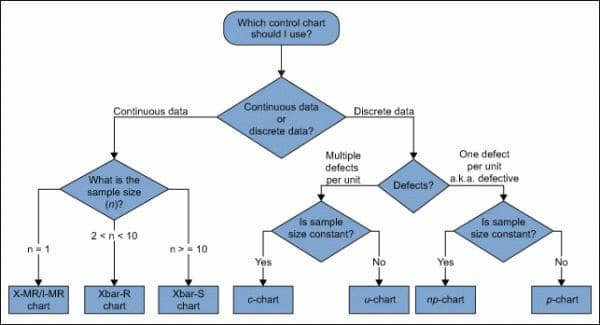
\includegraphics[scale=0.6]{pic/control-chart-decision-tree.jpg}
\caption{\textit{Control chart decision tree.}}
\end{figure}

\section{Pareto Chart in Statistical Quality Control}

A \textbf{Pareto chart} is a bar graph that displays the frequency or impact of problems or defects in descending order, alongside a cumulative percentage line. It is based on the \textbf{Pareto principle} (also known as the 80/20 rule), which suggests that roughly 80\% of the problems arise from 20\% of the causes.

In SQC, Pareto charts help prioritize improvement efforts by identifying the most significant sources of defects or errors.

\textbf{Example}: Suppose a factory inspects 1000 products and records the number of occurrences for various types of defects. The data is shown below:

\begin{table}[H]
\centering
\begin{tabular}{l|c|c|c}
\toprule
\textbf{Defect Type} & \textbf{Frequency} & \textbf{Percentage (\%)} & \textbf{Cumulative \%} \\
\midrule
Surface Scratch & 300 & 30.0 & 30.0 \\
Paint Defect & 250 & 25.0 & 55.0 \\
Loose Screw & 150 & 15.0 & 70.0 \\
Crack & 100 & 10.0 & 80.0 \\
Missing Label & 80 & 8.0 & 88.0 \\
Bent Part & 70 & 7.0 & 95.0 \\
Other & 50 & 5.0 & 100.0 \\
\bottomrule
\end{tabular}
\caption{\textit{Frequency of Defect Types in Production.}}
\end{table}

\vspace{0.5cm}

The Pareto chart for the above data is shown below:

\begin{figure}[H]
  \centering
  \begin{tikzpicture}
    % First axis: bars using numeric x
    \begin{axis}[
        name=baraxis,
        ybar,
        ylabel={Frequency},
        xlabel={Defect Type},
        % numeric x positions
        xmin=0.5, xmax=7.5,
        ymin=0, ymax=350,
        xtick={1,2,3,4,5,6,7},
        xticklabels={
          Surface Scratch,
          Paint Defect,
          Loose Screw,
          Crack,
          Missing Label,
          Bent Part,
          Other
        },
        xticklabel style={rotate=45, anchor=east,font=\small},
        bar width=12pt,
        enlarge x limits=0.15,
        axis y line*=left,
        axis x line*=bottom,
        nodes near coords,
        every node near coord/.append style={font=\small},
        width=12cm,
        height=7cm, thick
    ]
      \addplot+[fill=blue!30] coordinates {
        (1,300) (2,250) (3,150) (4,100) (5,80) (6,70) (7,50)
      };
    \end{axis}

    % Second axis: cumulative percentage on right
    \begin{axis}[
        at={(baraxis.outer north east)},
        anchor={north east},
        axis y line*=right,
        axis x line=none,
        xmin=0.5, xmax=7.5,
        ymin=0, ymax=110,
        ylabel={Cumulative \%},
        ytick={0,20,...,100},
        width=12cm,
        height=7cm,
        nodes near coords,
        every node near coord/.append style={font=\small, above},
        thick
    ]
      \addplot+[mark=*, very thick, black] coordinates {
        (1.7,30) (2.46,55) (3.19,70) (4,80) (4.75,88) (5.55,95) (6.27,100)
      };
    \end{axis}
  \end{tikzpicture}
  \caption{\textit{Pareto Chart for Defect Types.}}
\end{figure}

\textbf{Interpretation}

From the Pareto chart, it is evident that the majority of the defects (70\%) come from the first three types: surface scratches, paint defects, and loose screws. Therefore, quality improvement efforts should focus on these issues first to achieve the greatest impact with minimal effort.



\section{Process Capability Analysis}

Process capability analysis assesses whether a process can meet specifications consistently.

\subsection{Process Capability Indices}

\subsubsection{$C_p$ Index}

The $C_p$ index measures the potential capability of a process:
$$C_p = \frac{USL - LSL}{6\sigma}$$

where USL = Upper Specification Limit, LSL = Lower Specification Limit, and $\sigma$ is the process standard deviation.

\subsubsection{$C_{pk}$ Index}

The $C_{pk}$ index considers process centering:
$$C_{pk} = \min\left(\frac{USL - \mu}{3\sigma}, \frac{\mu - LSL}{3\sigma}\right)$$

where $\mu$ is the process mean.

\textbf{Interpretation}

\begin{table}[H]
\centering
\caption{Process Capability Interpretation}
\begin{tabular}{cc}
\toprule
$C_{pk}$ Value & Process Capability \\
\midrule
$C_{pk} \geq 2.0$ & Excellent \\
$1.33 \leq C_{pk} < 2.0$ & Adequate \\
$1.0 \leq C_{pk} < 1.33$ & Marginal \\
$C_{pk} < 1.0$ & Inadequate \\
\bottomrule
\end{tabular}
\end{table}

\subsubsection{Example: Process Capability Calculation}

A process has specifications: LSL = 95, USL = 105
Process data: $\mu = 100$, $\sigma = 1.5$

$$C_p = \frac{105 - 95}{6 \times 1.5} = \frac{10}{9} = 1.11$$

$$C_{pk} = \min\left(\frac{105 - 100}{3 \times 1.5}, \frac{100 - 95}{3 \times 1.5}\right) = \min(1.11, 1.11) = 1.11$$

The process is marginally capable but centered.

\section{Acceptance Sampling}

Acceptance sampling is a statistical method used to determine whether to accept or reject a batch of products based on inspection of a sample.

\subsection{Single Sampling Plans}

A single sampling plan is characterized by $(n, c)$ where:
\begin{itemize}
    \item $n$ = sample size
    \item $c$ = acceptance number
\end{itemize}

Decision rule: Accept the lot if the number of defective items $d \leq c$

\subsection{Operating Characteristic (OC) Curve}

The OC curve shows the probability of accepting a lot as a function of the lot fraction defective $p$.

For a binomial distribution:
$$P_a(p) = \sum_{d=0}^{c} \binom{n}{d} p^d (1-p)^{n-d}$$

\subsubsection{Example: OC Curve Calculation}

For a sampling plan $(n=50, c=2)$:

\begin{figure}[H]
\centering
\begin{tikzpicture}[scale=0.8]
\begin{axis}[
    title={Operating Characteristic Curve},
    xlabel={Fraction Defective (p)},
    ylabel={Probability of Acceptance},
    xmin=0, xmax=0.2,
    ymin=0, ymax=1,
    grid=major
]
\addplot[blue, thick, smooth] coordinates {
    (0,1) (0.02,0.92) (0.04,0.68) (0.06,0.42) (0.08,0.24) (0.10,0.12) (0.12,0.06) (0.14,0.03) (0.16,0.01) (0.18,0.005) (0.20,0.002)
};
\end{axis}
\end{tikzpicture}
\end{figure}

\subsection{Producer's and Consumer's Risks}

\begin{itemize}
    \item \textbf{Producer's Risk ($\alpha$)}: Probability of rejecting a good lot
    \item \textbf{Consumer's Risk ($\beta$)}: Probability of accepting a bad lot
\end{itemize}

Typically:
\begin{itemize}
    \item AQL (Acceptable Quality Level): $\alpha = 0.05$
    \item LTPD (Lot Tolerance Percent Defective): $\beta = 0.10$
\end{itemize}

\section{Reliability and Life Testing}

Reliability is the probability that a system performs successfully during a specified time interval under specified conditions.

\subsection{Reliability Function}

The reliability function $R(t)$ is defined as:
$$R(t) = P(T > t) = 1 - F(t)$$

where $T$ is the random variable representing time to failure and $F(t)$ is the cumulative distribution function.

\subsection{Failure Rate Function}

The hazard rate or failure rate function $h(t)$ is:
$$h(t) = \frac{f(t)}{R(t)} = \frac{f(t)}{1-F(t)}$$

where $f(t)$ is the probability density function.

\subsection{Common Life Distributions}

\subsubsection{Exponential Distribution}

For constant failure rate $\lambda$:
$$f(t) = \lambda e^{-\lambda t}, \quad t \geq 0$$
$$R(t) = e^{-\lambda t}$$
$$h(t) = \lambda$$

Mean Time To Failure (MTTF):
$$MTTF = \frac{1}{\lambda}$$

\subsubsection{Weibull Distribution}

The Weibull distribution is widely used in reliability analysis:
$$f(t) = \frac{\beta}{\eta}\left(\frac{t}{\eta}\right)^{\beta-1} e^{-(t/\eta)^{\beta}}$$

where $\beta$ is the shape parameter and $\eta$ is the scale parameter.

$$R(t) = e^{-(t/\eta)^{\beta}}$$

$$h(t) = \frac{\beta}{\eta}\left(\frac{t}{\eta}\right)^{\beta-1}$$

\subsubsection{Bathtub Curve}

The bathtub curve describes the failure rate pattern over product lifetime:

\begin{figure}[H]
\centering
\begin{tikzpicture}[scale=0.8]
\begin{axis}[
    title={Bathtub Curve},
    xlabel={Time},
    ylabel={Failure Rate},
    xmin=0, xmax=10,
    ymin=0, ymax=3,
    grid=major,
    xtick={2,6,8},
    xticklabels={Early Life, Useful Life, Wear-out}
]
\addplot[blue, thick, smooth] coordinates {
    (0,2.5) (0.5,2.0) (1,1.5) (1.5,1.2) (2,1.0) (3,0.8) (4,0.7) (5,0.6) (6,0.5) (7,0.6) (8,1.0) (9,1.8) (10,3.0)
};
\node at (axis cs:1,2.2) {Infant Mortality};
\node at (axis cs:4,0.3) {Random Failures};
\node at (axis cs:8.5,2.5) {Wear-out};
\end{axis}
\end{tikzpicture}
\end{figure}

\subsection{Life Testing}

\subsubsection{Complete Testing}

All units are tested until failure. Provides complete information but time-consuming.

\subsubsection{Censored Testing}

\textbf{Type I Censoring}: Testing stops at predetermined time $t_0$

\textbf{Type II Censoring}: Testing stops after predetermined number of failures $r$

\subsubsection{Accelerated Life Testing}

Testing under elevated stress conditions to accelerate failures.

Arrhenius model:
$$\lambda(T) = A e^{E_a/(kT)}$$

where $T$ is temperature, $E_a$ is activation energy, $k$ is Boltzmann constant, and $A$ is a constant.

\subsection{System Reliability}

\subsubsection{Series System}

For a series system with $n$ components:
$$R_s(t) = \prod_{i=1}^{n} R_i(t)$$

\subsubsection{Parallel System}

For a parallel system with $n$ components:
$$R_p(t) = 1 - \prod_{i=1}^{n} [1 - R_i(t)]$$

\subsubsection{Example: System Reliability Calculation}

Consider a system with 3 components in series, each with reliability $R(t) = e^{-0.001t}$:

$$R_s(t) = [e^{-0.001t}]^3 = e^{-0.003t}$$

For the same components in parallel:
$$R_p(t) = 1 - [1 - e^{-0.001t}]^3$$

\begin{figure}[H]
\centering
\begin{tikzpicture}[scale=0.8]
\begin{axis}[
    title={System Reliability Comparison},
    xlabel={Time (hours)},
    ylabel={Reliability},
    xmin=0, xmax=2000,
    ymin=0, ymax=1,
    grid=major,
    legend pos=north east
]
\addplot[blue, thick] coordinates {(0,1) (200,0.82) (400,0.67) (600,0.55) (800,0.45) (1000,0.37) (1200,0.30) (1400,0.25) (1600,0.20) (1800,0.17) (2000,0.14)};
\addplot[red, thick] coordinates {(0,1) (200,0.67) (400,0.45) (600,0.30) (800,0.20) (1000,0.14) (1200,0.09) (1400,0.06) (1600,0.04) (1800,0.03) (2000,0.02)};
\addplot[green, thick] coordinates {(0,1) (200,0.9997) (400,0.9988) (600,0.9973) (800,0.9955) (1000,0.9933) (1200,0.9909) (1400,0.9882) (1600,0.9853) (1800,0.9822) (2000,0.9789)};
\legend{Single Component, Series System, Parallel System}
\end{axis}
\end{tikzpicture}
\end{figure}

\section{Conclusion}

Statistical Quality Control provides a comprehensive framework for monitoring, controlling, and improving quality in manufacturing and service processes. The key principles include:

\begin{itemize}
    \item Use of statistical methods to distinguish between common and special causes of variation
    \item Implementation of control charts for continuous monitoring
    \item Application of process capability analysis to ensure specifications are met
    \item Employment of acceptance sampling for lot-by-lot decisions
    \item Utilization of statistical tools for quality improvement
    \item Application of reliability methods for long-term performance assessment
\end{itemize}

The successful implementation of SQC requires understanding of statistical concepts, proper data collection, and commitment to continuous improvement. These methods, when properly applied, lead to reduced variability, improved quality, and enhanced customer satisfaction.


\end{document}


